\chapter{Threshold outcomes for method selection}
\makeatletter\@mkboth{}{Appendix}\makeatother
The outcomes for the global and local thresholding methods being shortlisted with the sample images shown below in Figure \ref{appen-fig:shortlist_samples}.

\begin{figure}[ht!]
	\centering
	\subcaptionbox{Sample 1}{
\includegraphics[width=0.2\textwidth]{figs/appendix/method_shortlisting/CCCP_1C=1T=0.png}}
	\subcaptionbox{Sample 2}{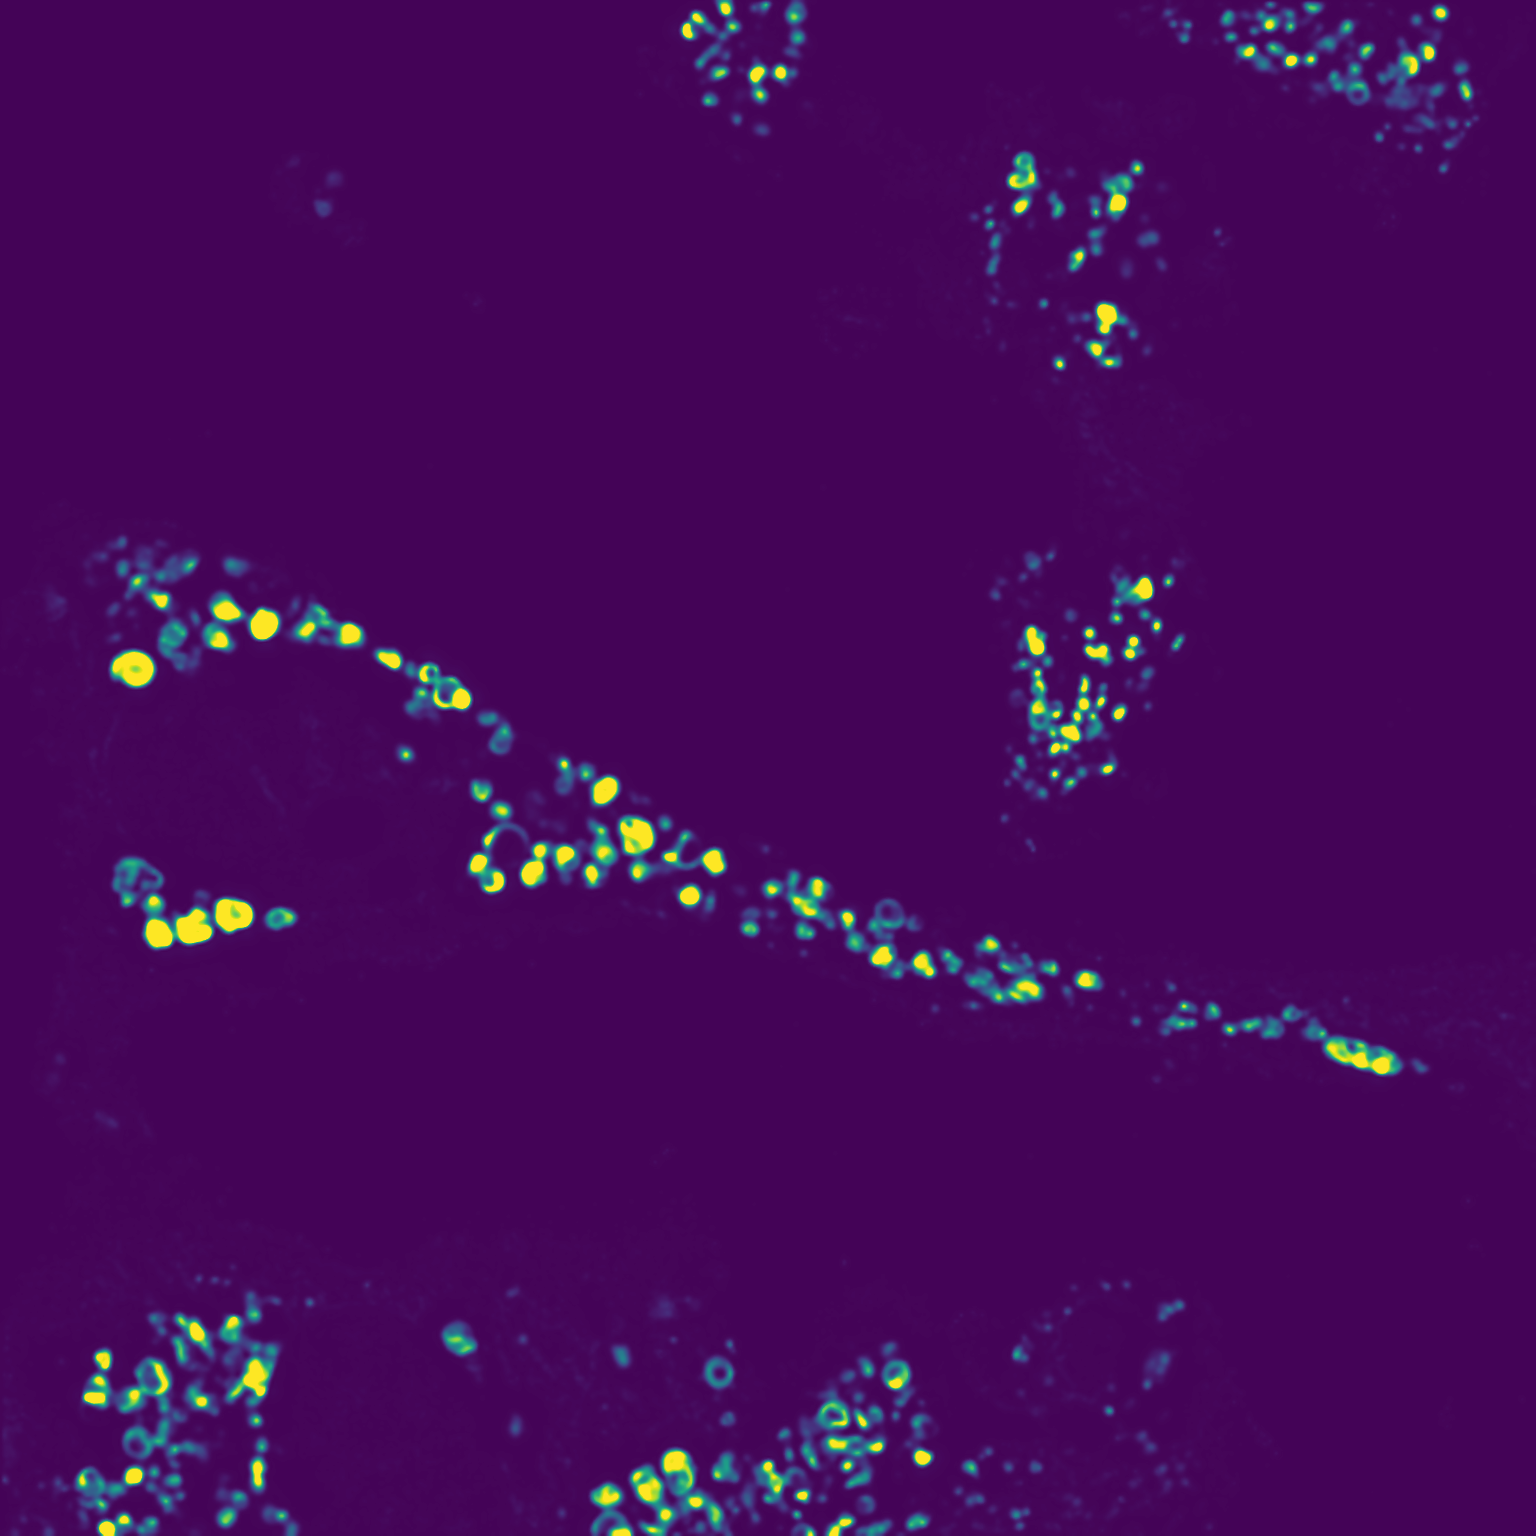
\includegraphics[width=0.2\textwidth]{figs/appendix/method_shortlisting/HML_4C=0.png}}
	\subcaptionbox{Sample 3}{
\includegraphics[width=0.2\textwidth]{figs/appendix/method_shortlisting/LML_3C=0.png}}
	\subcaptionbox{Sample 4}{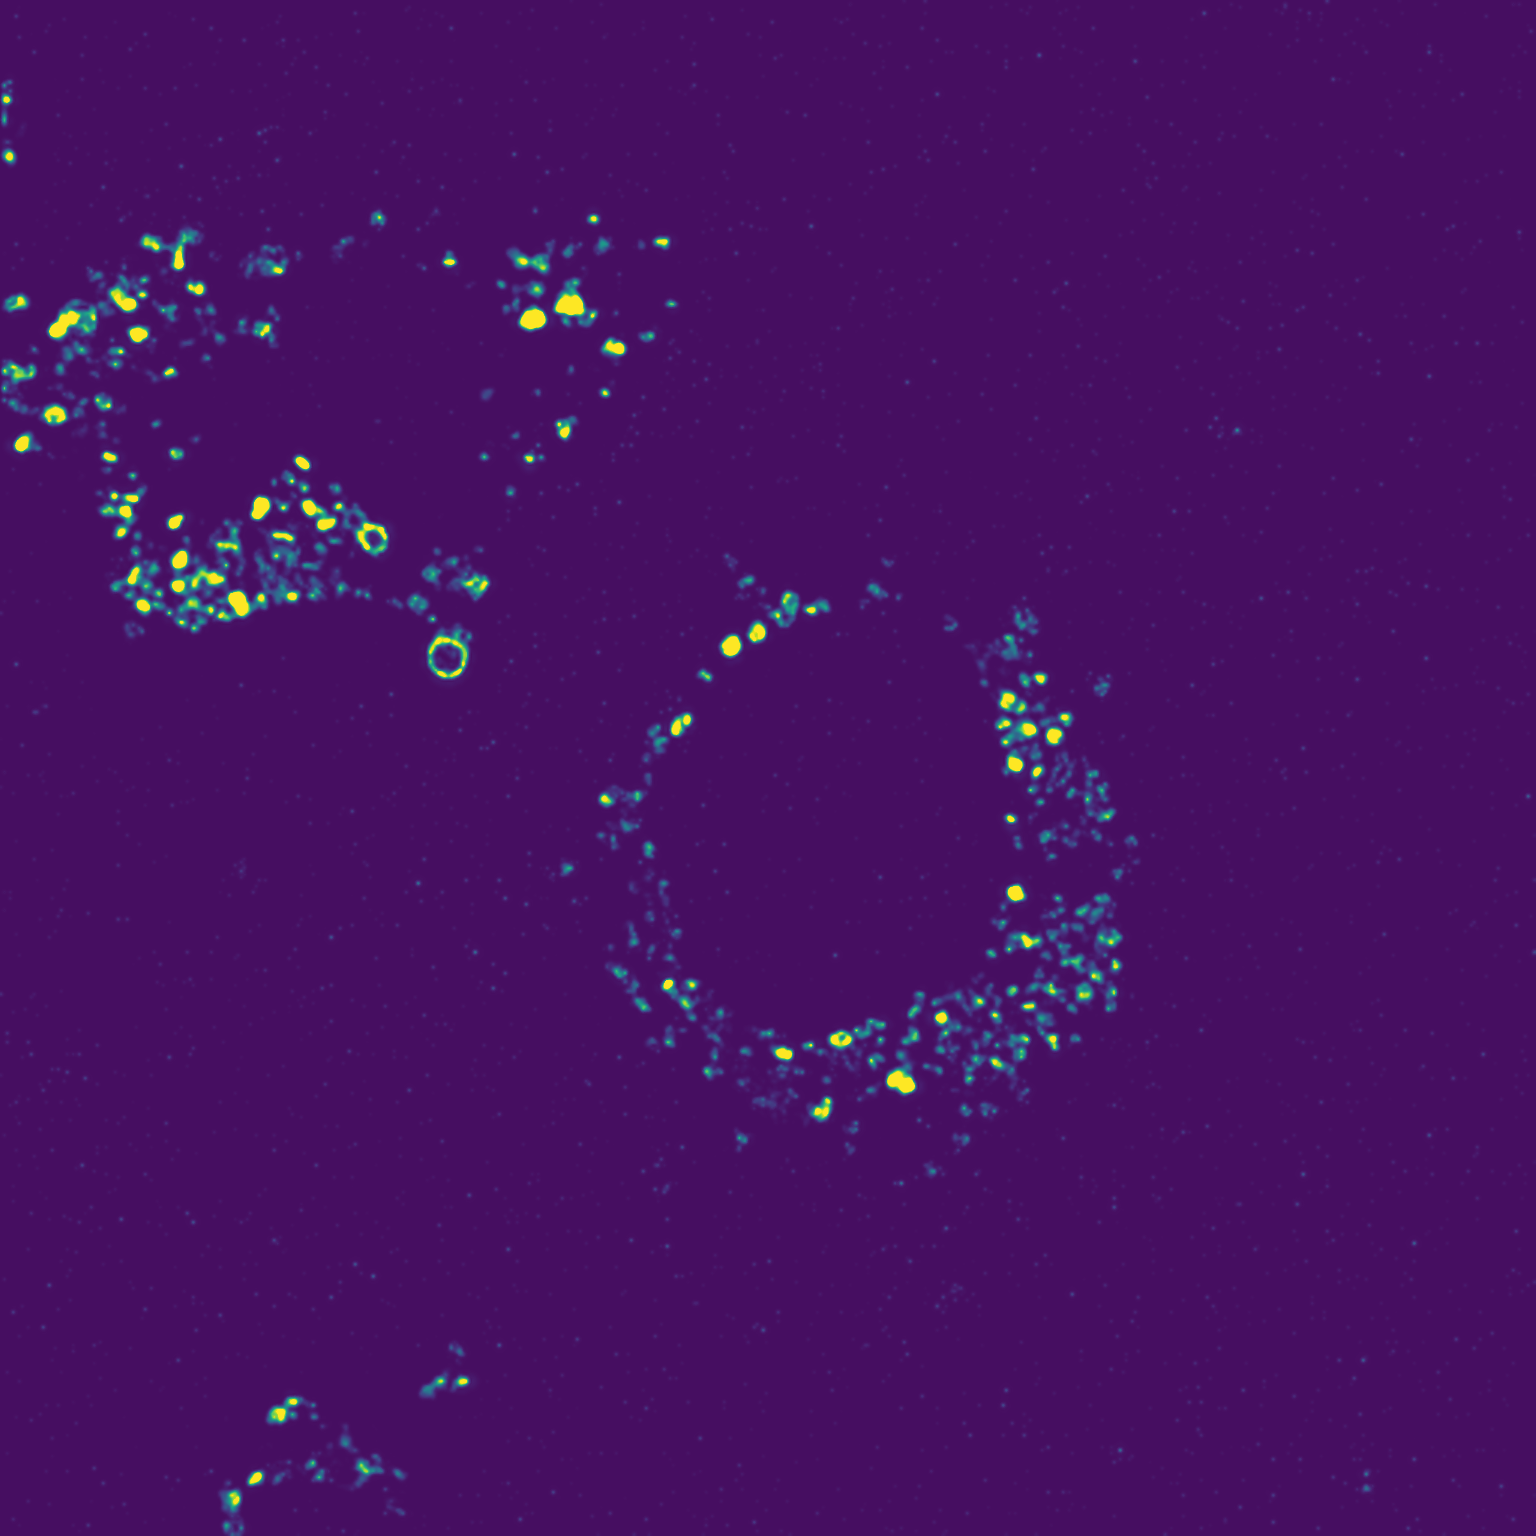
\includegraphics[width=0.2\textwidth]{figs/appendix/method_shortlisting/LML_4C=1.png}}
	\caption{Central slices of the pre-processed shortlisting samples prior to any thresholding}
	\label{appen-fig:shortlist_samples}
\end{figure}
\FloatBarrier
\section{Global threshold outcomes of shortlist samples}\label{appen_sec:global_shortlist}

\begin{figure}[ht!]
	\centering
	\subcaptionbox{Sample 1}{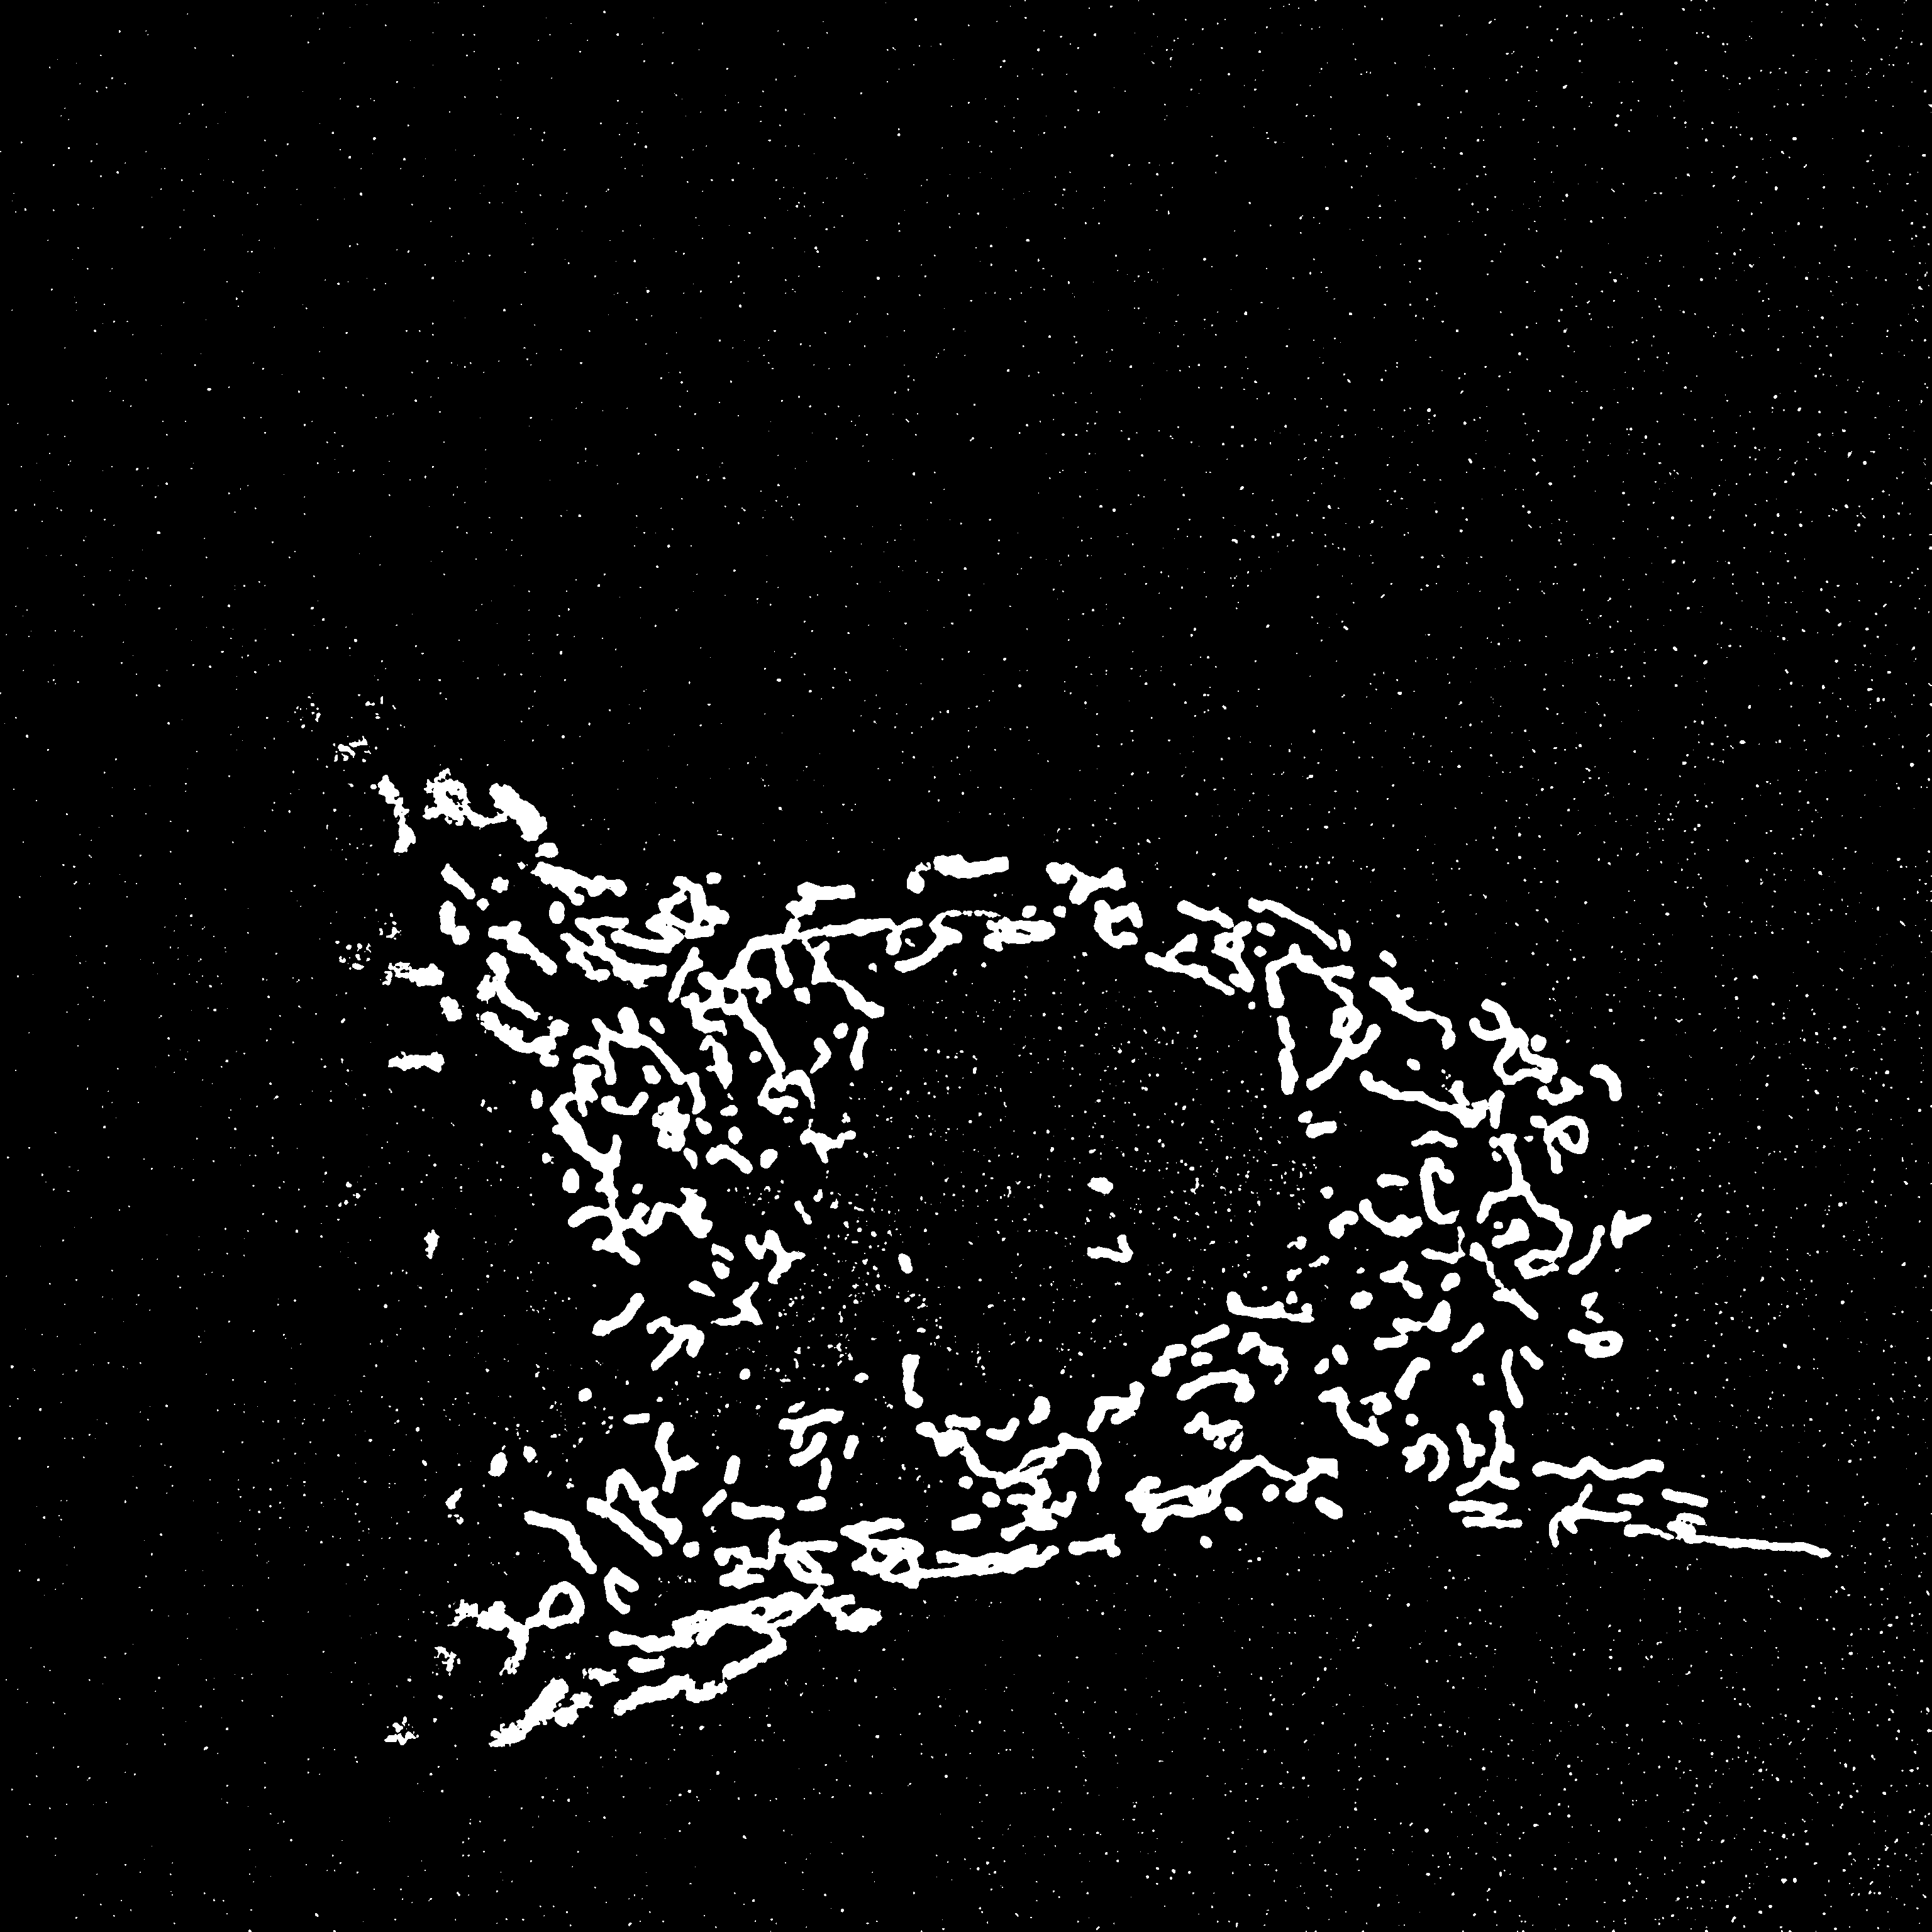
\includegraphics[width=0.2\textwidth]{figs/appendix/method_shortlisting/global_testing/Huang_CCCP_1C=1T=0.png}}
	\subcaptionbox{Sample 2}{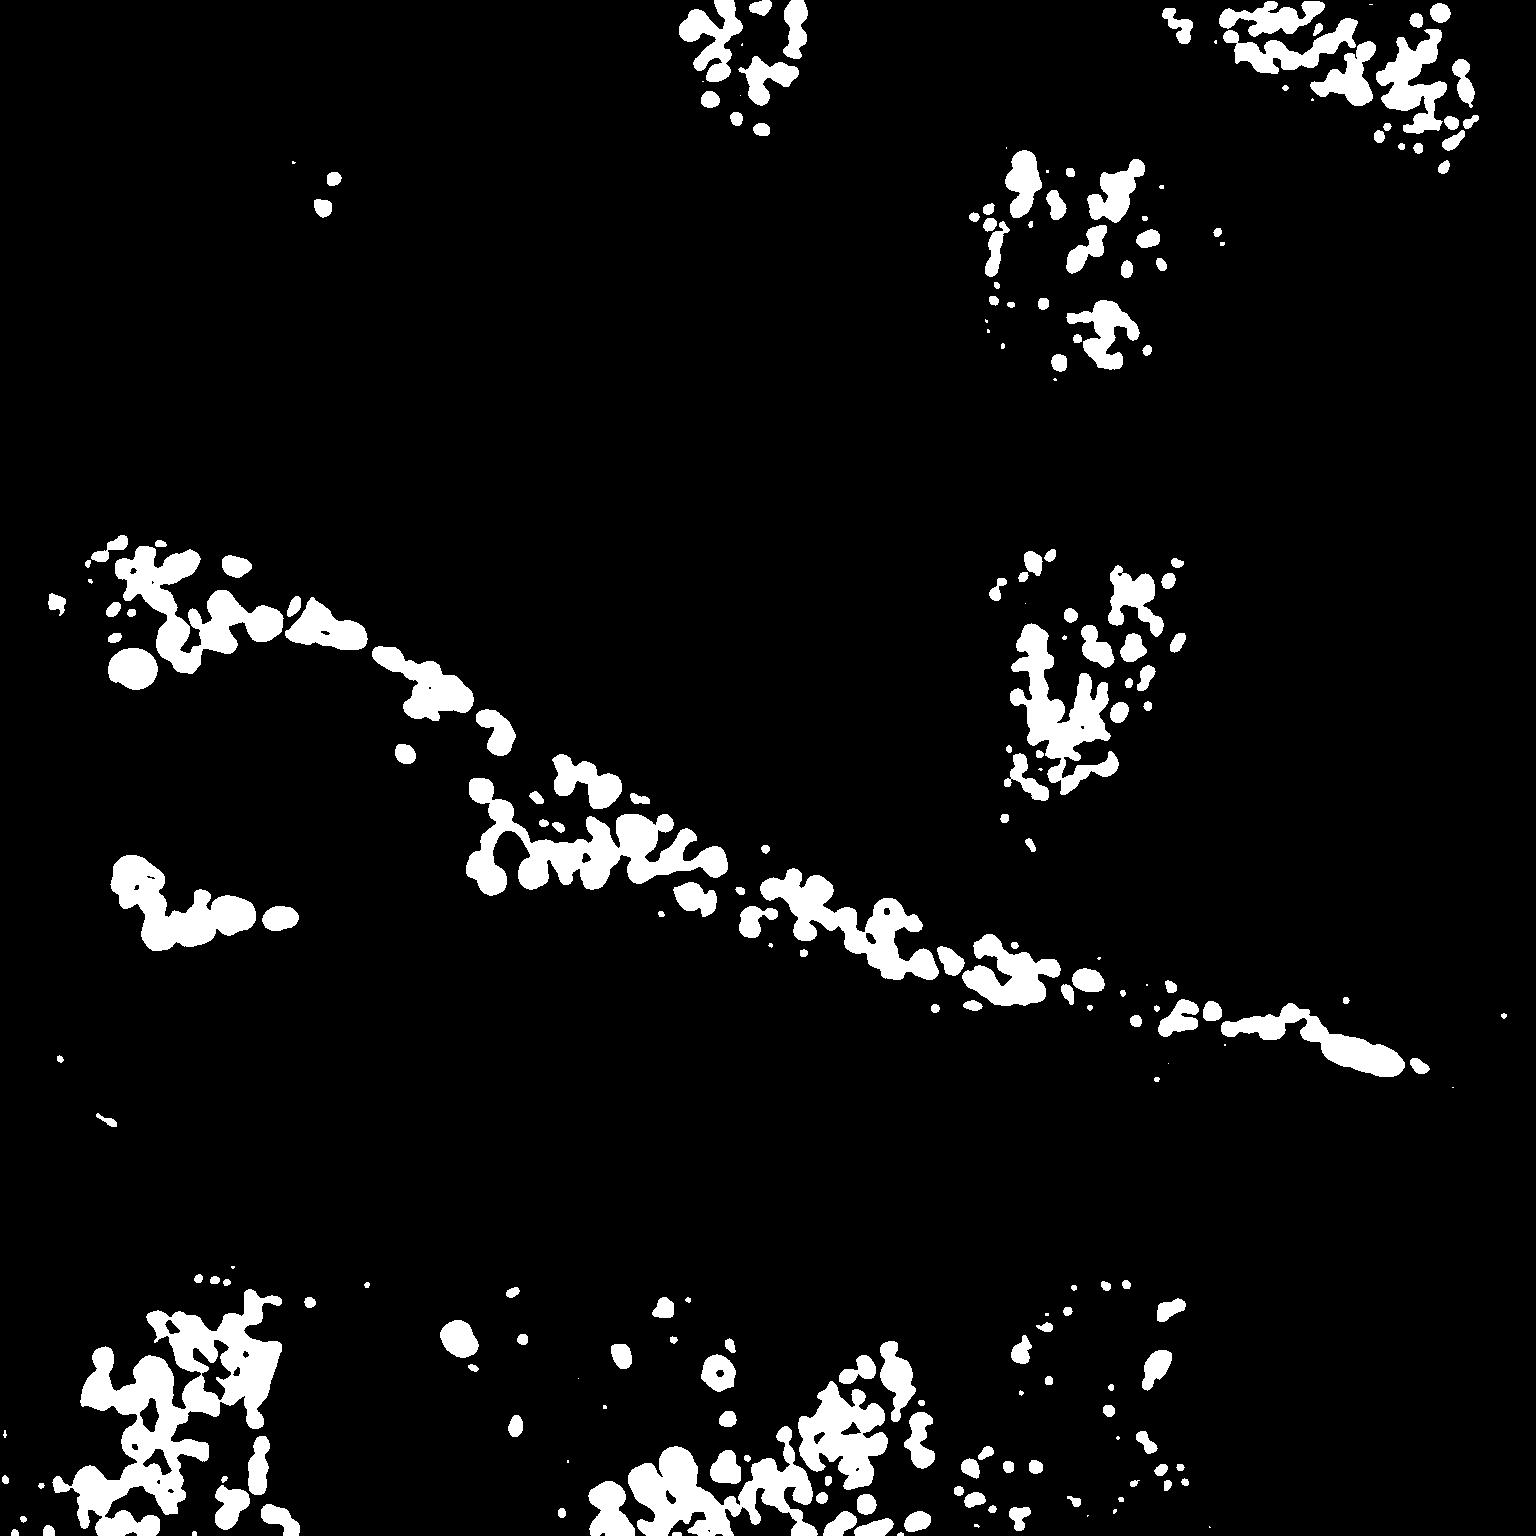
\includegraphics[width=0.2\textwidth]{figs/appendix/method_shortlisting/global_testing/Huang_HML_4C=0.png}}
	\subcaptionbox{Sample 3}{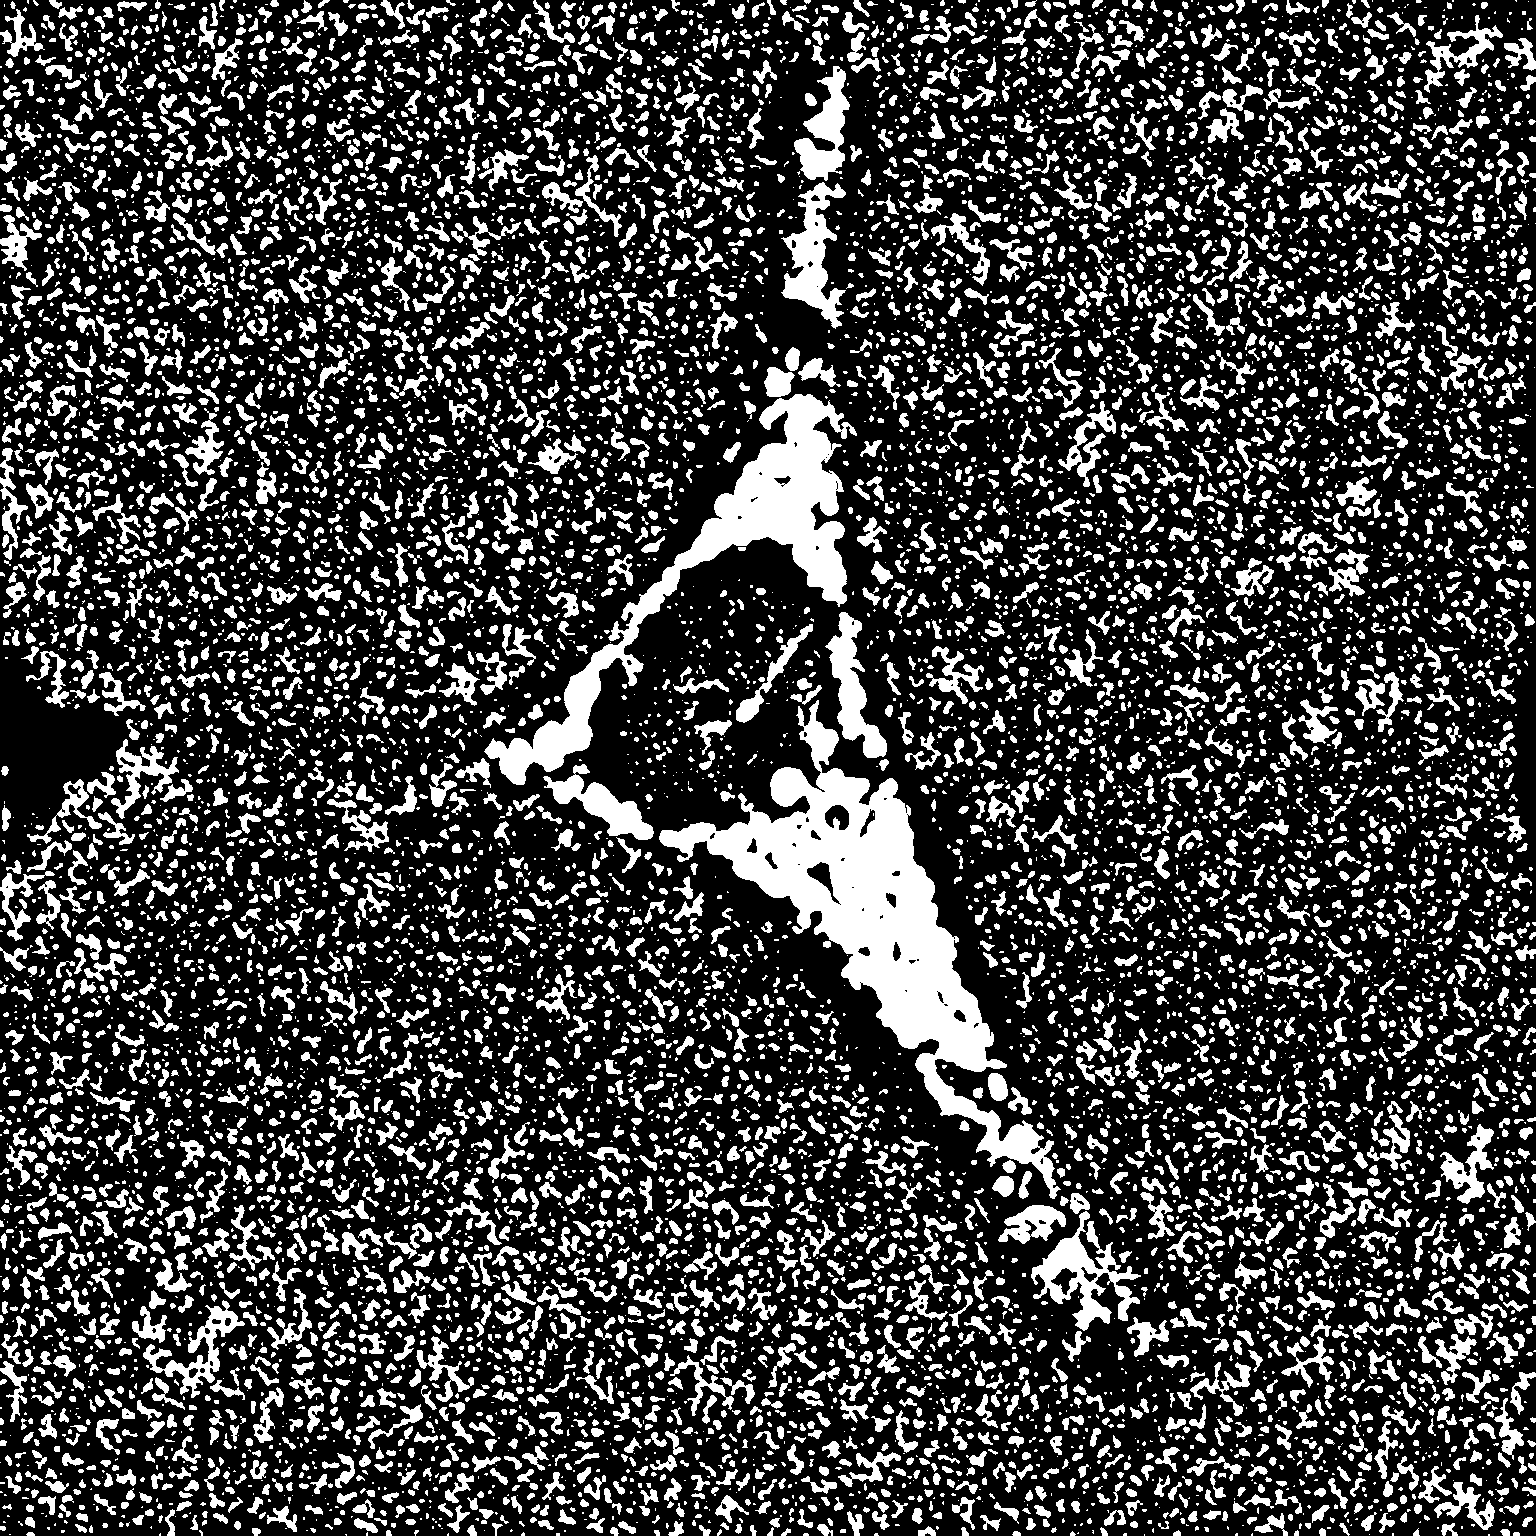
\includegraphics[width=0.2\textwidth]{figs/appendix/method_shortlisting/global_testing/Huang_LML_3C=0.png}}
	\subcaptionbox{Sample 4}{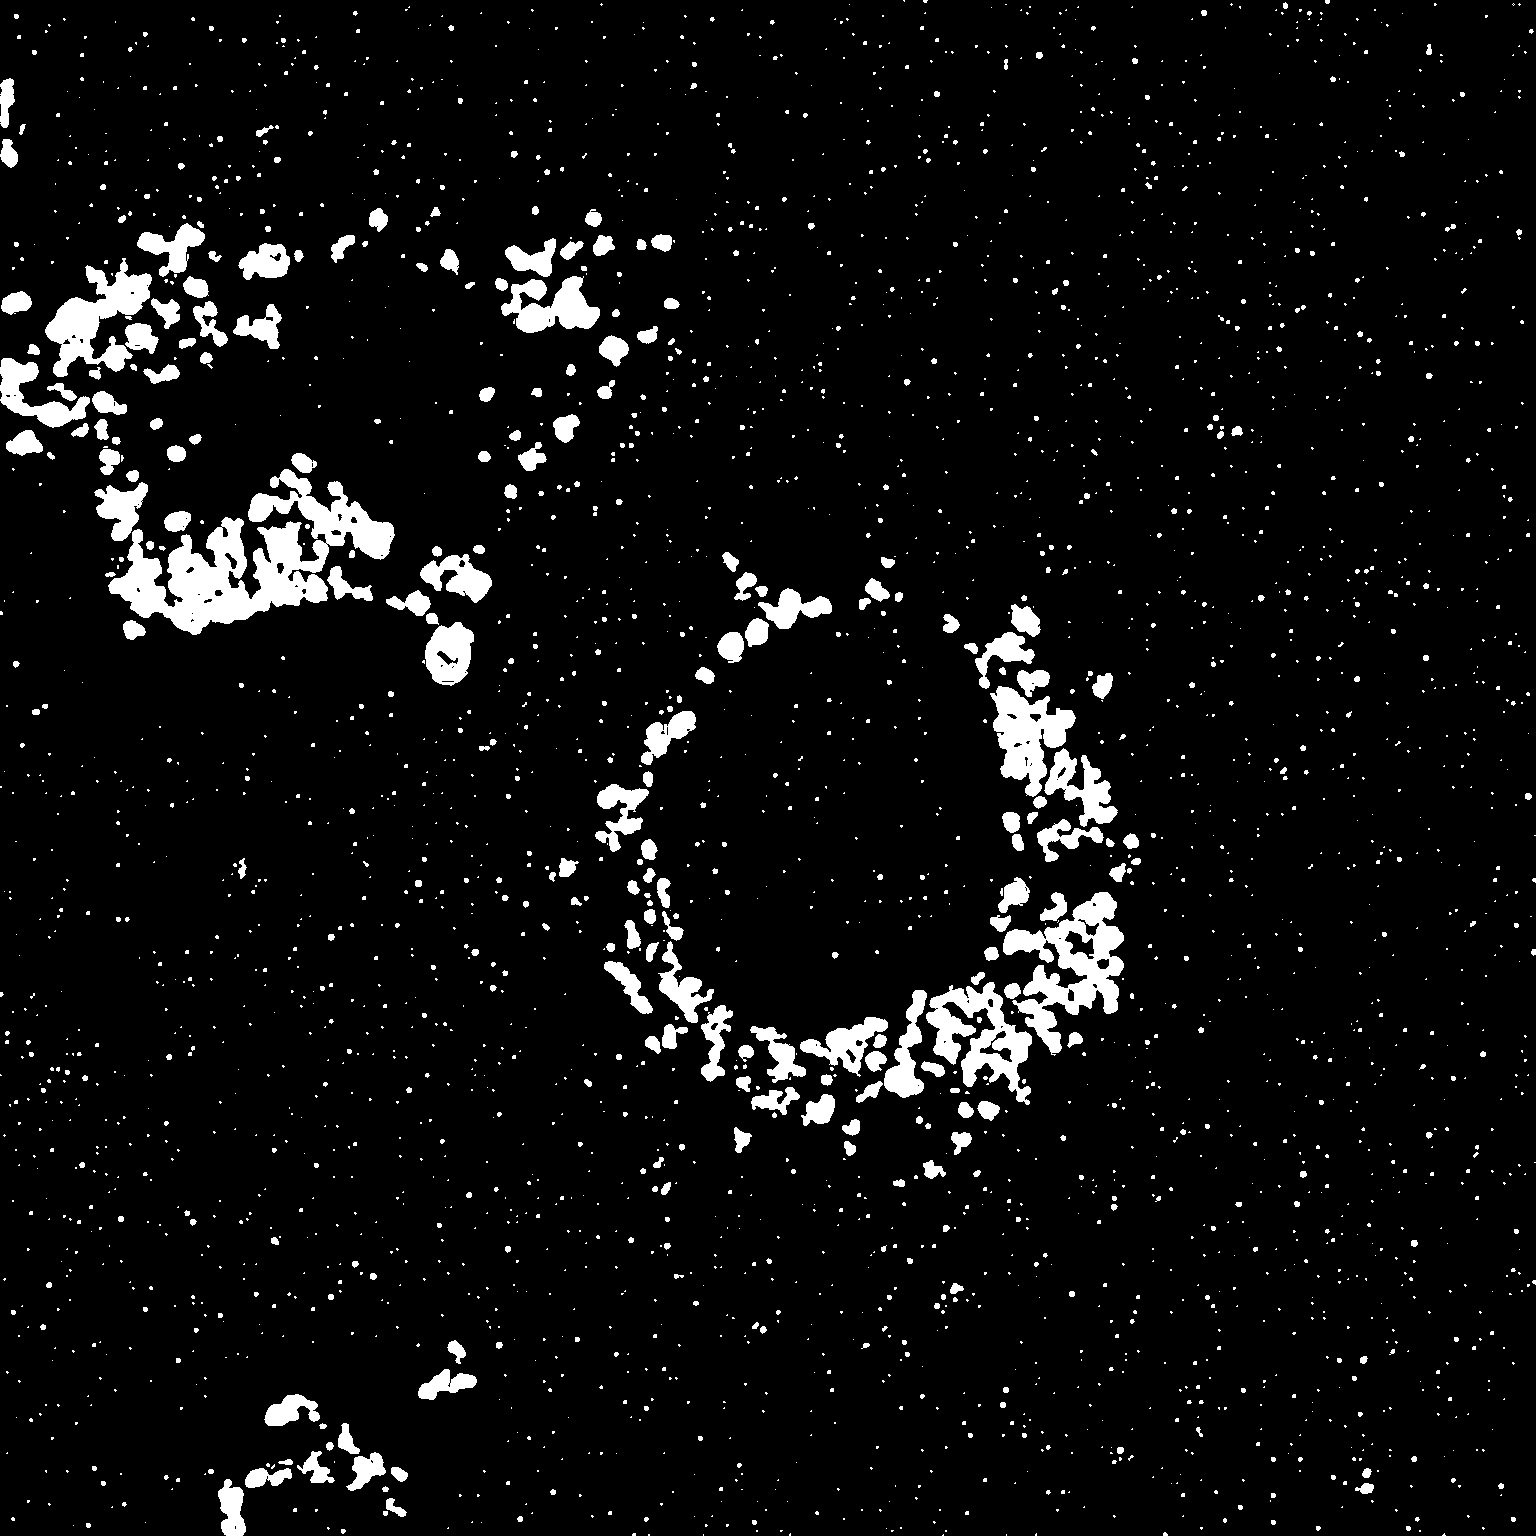
\includegraphics[width=0.2\textwidth]{figs/appendix/method_shortlisting/global_testing/Huang_LML_4C=1.png}}
	\label{append-fig:huang_short}
	\caption{Huang threshold outcomes for the shortlist sample images}
\end{figure}

\begin{figure}[ht!]
	\centering
	\subcaptionbox{Sample 1}{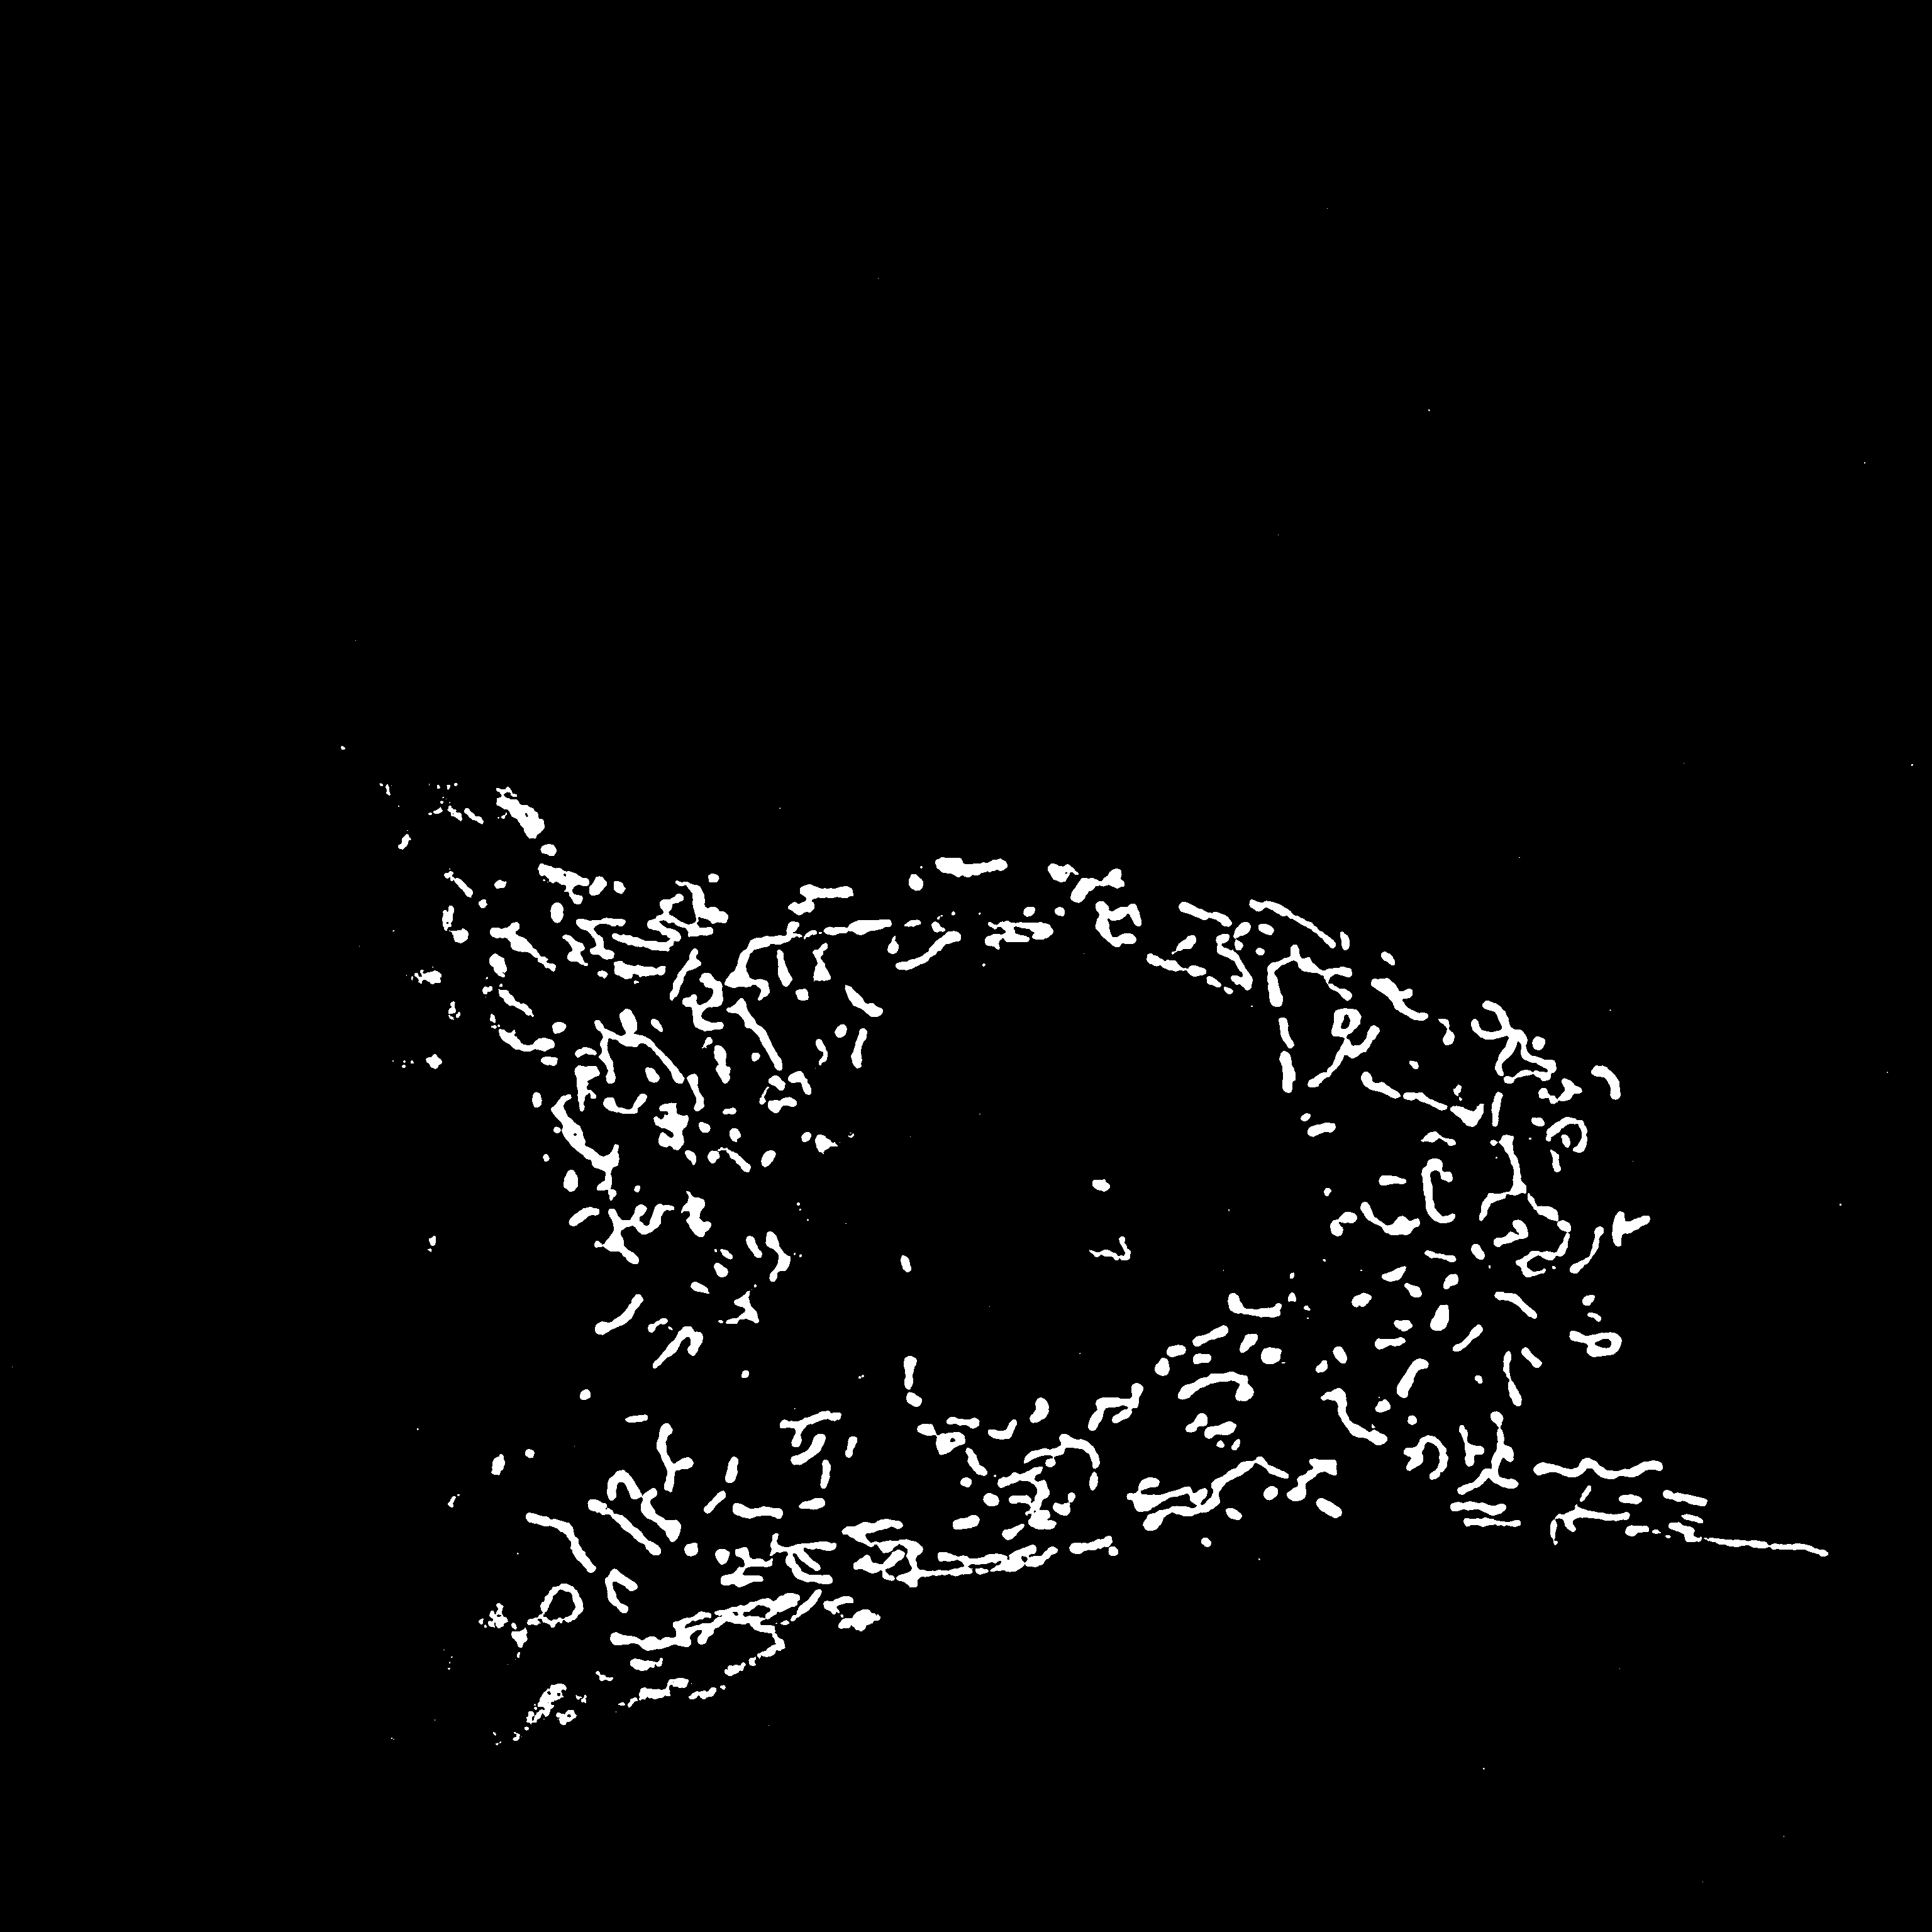
\includegraphics[width=0.2\textwidth]{figs/appendix/method_shortlisting/global_testing/Huang2_CCCP_1C=1T=0.png}}
	\subcaptionbox{Sample 2}{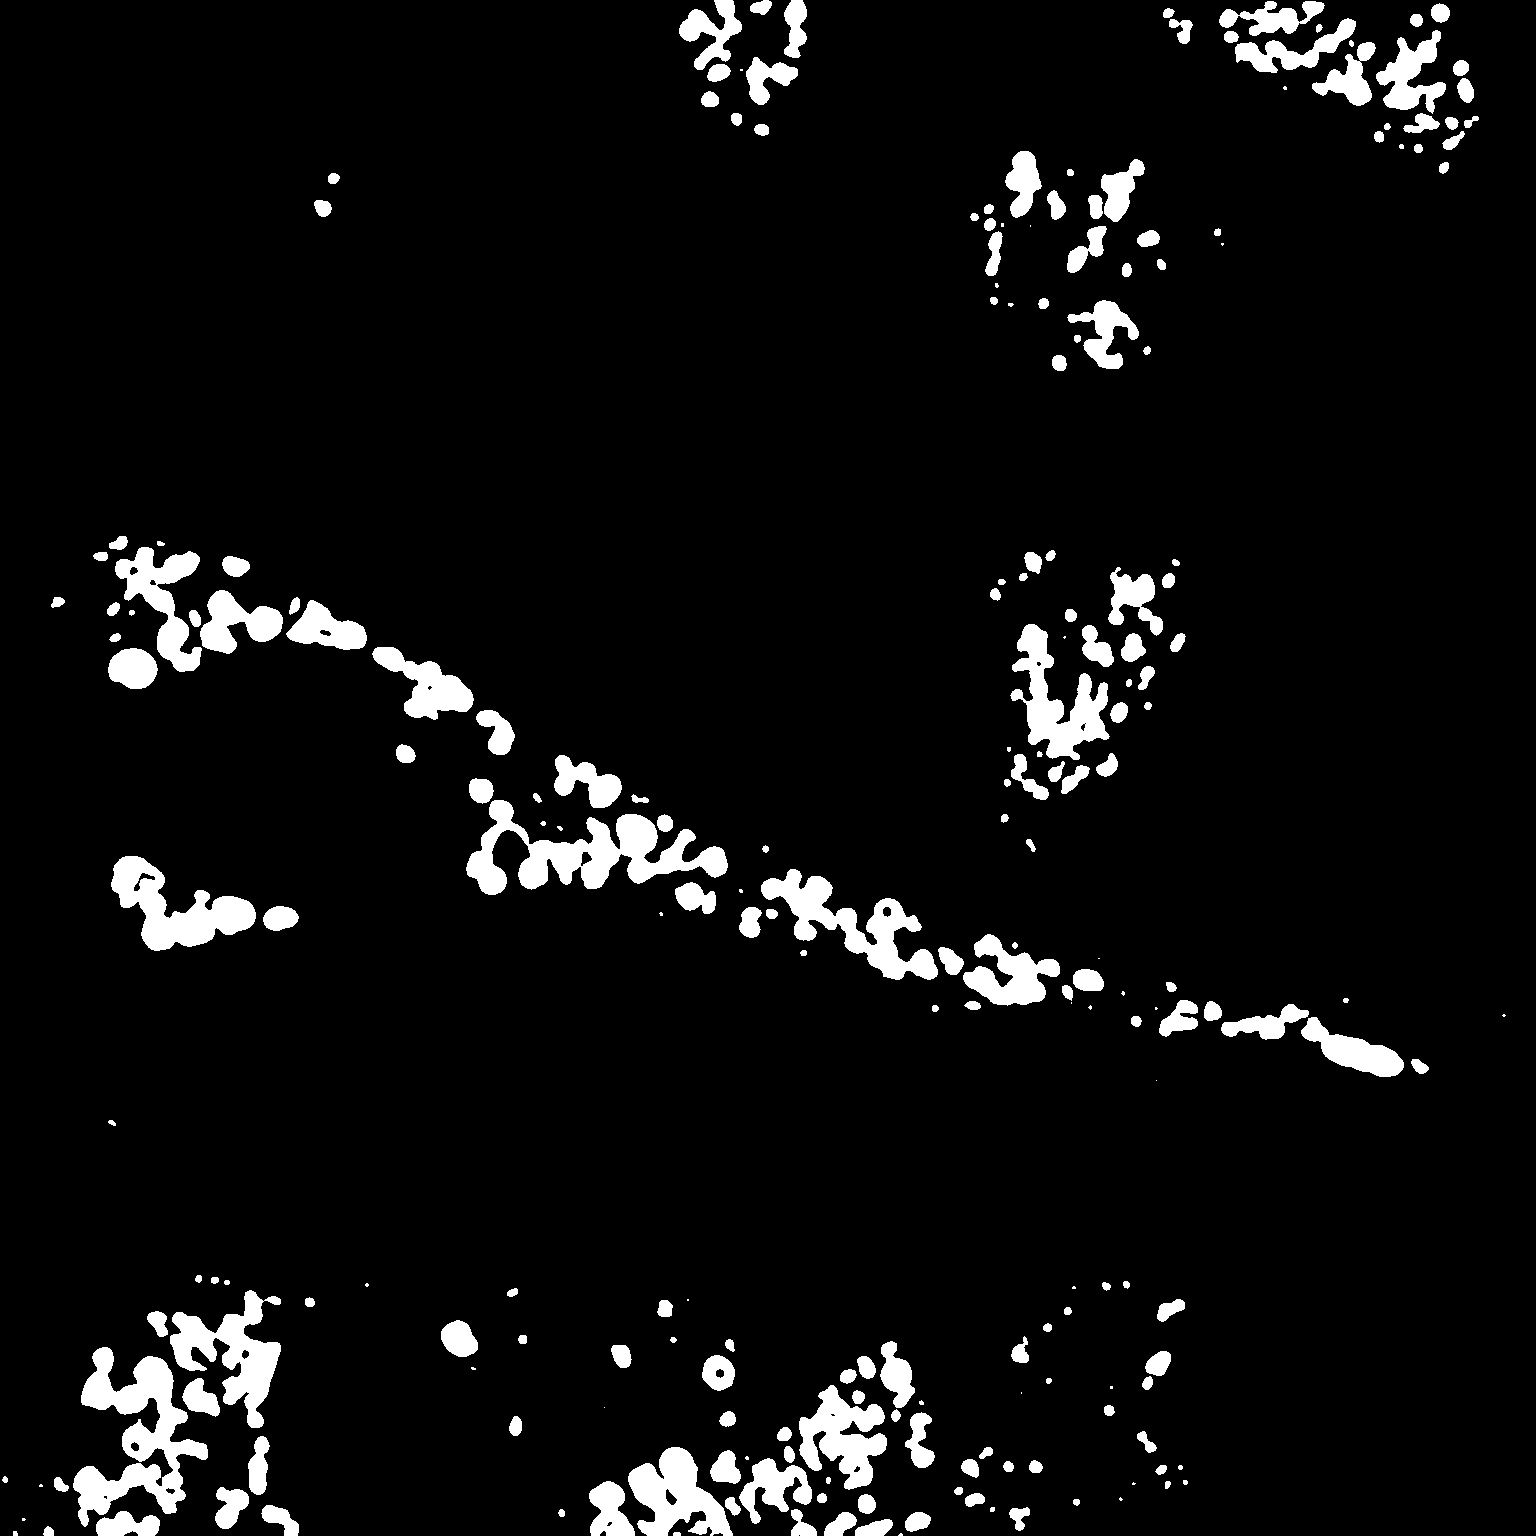
\includegraphics[width=0.2\textwidth]{figs/appendix/method_shortlisting/global_testing/Huang2_HML_4C=0.png}}
	\subcaptionbox{Sample 3}{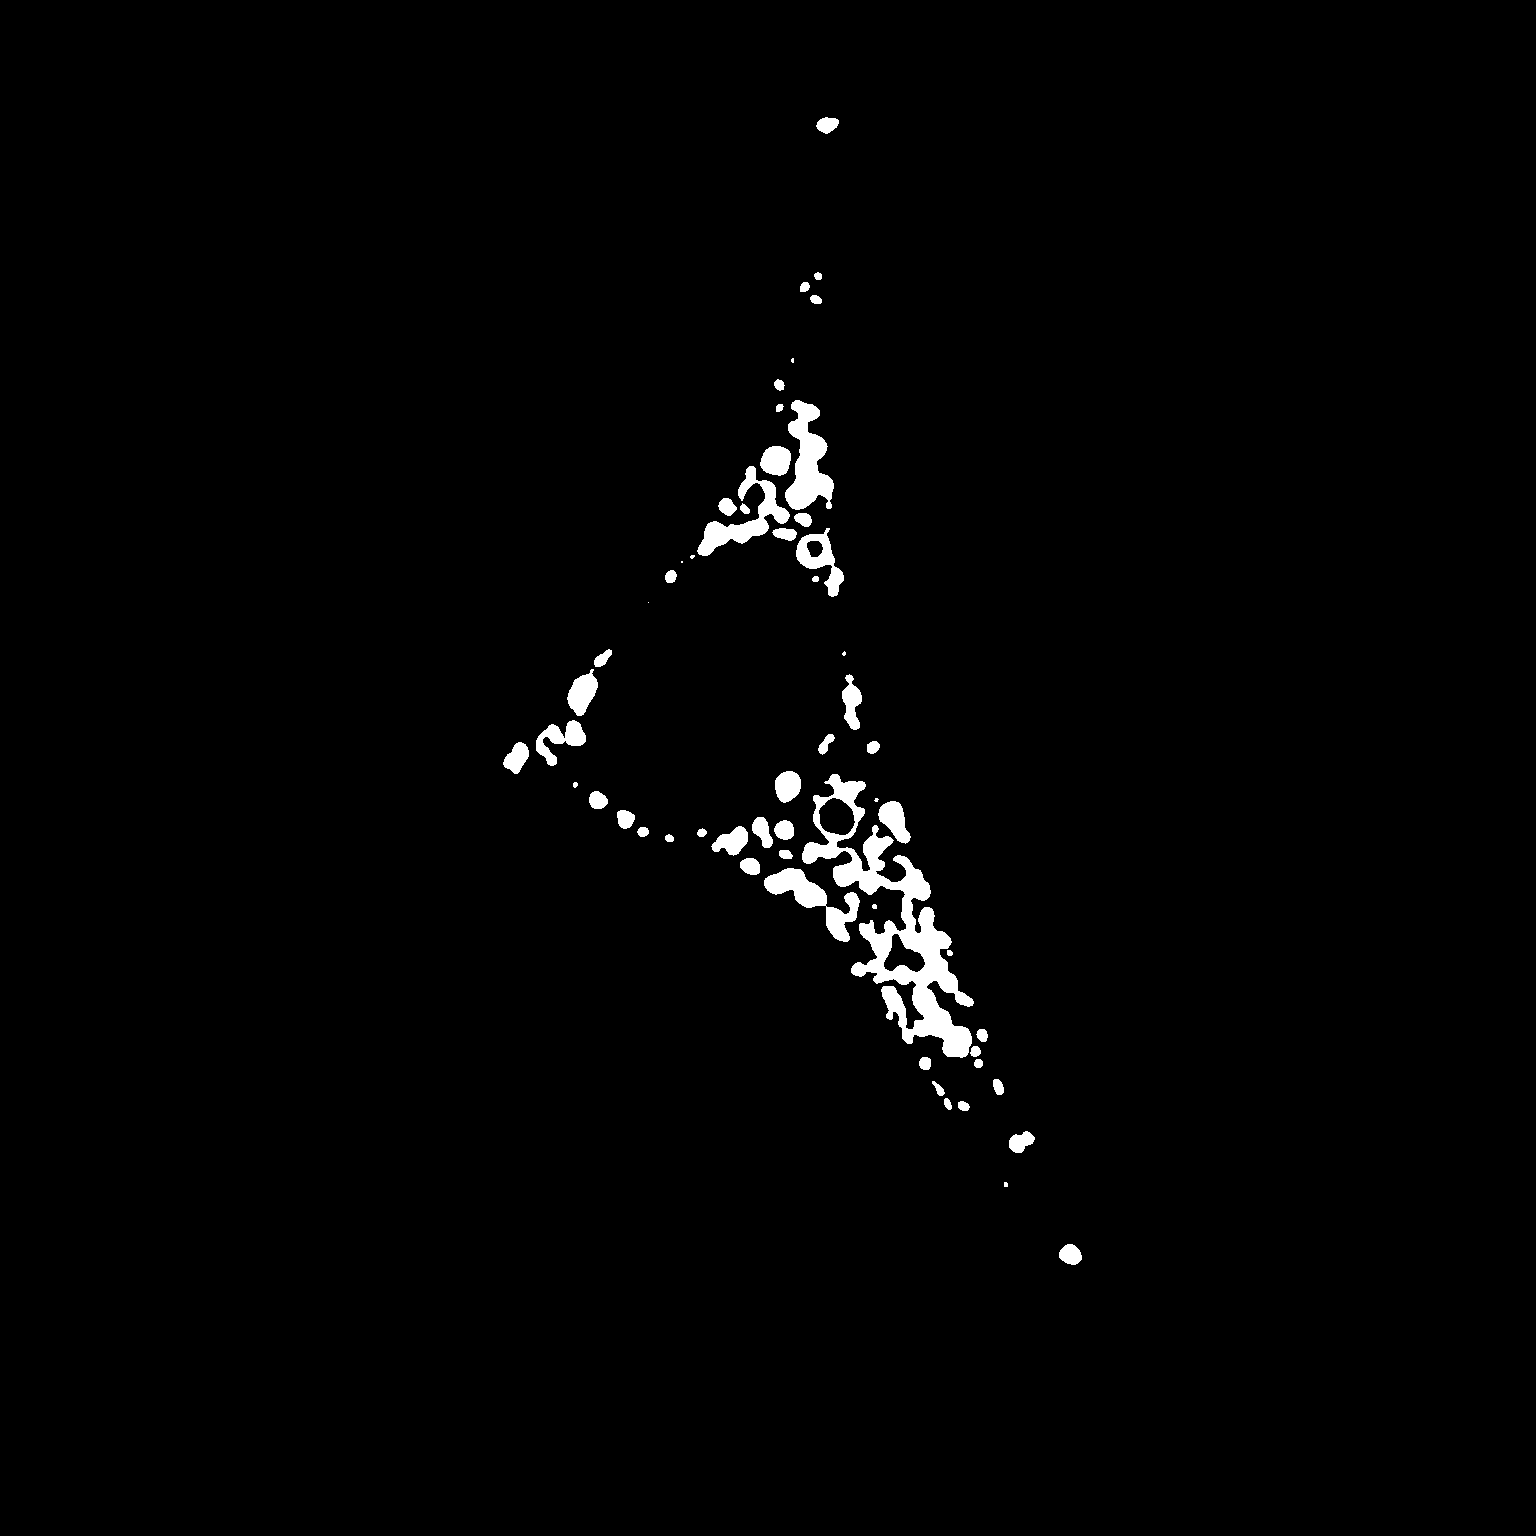
\includegraphics[width=0.2\textwidth]{figs/appendix/method_shortlisting/global_testing/Huang2_LML_3C=0.png}}
	\subcaptionbox{Sample 4}{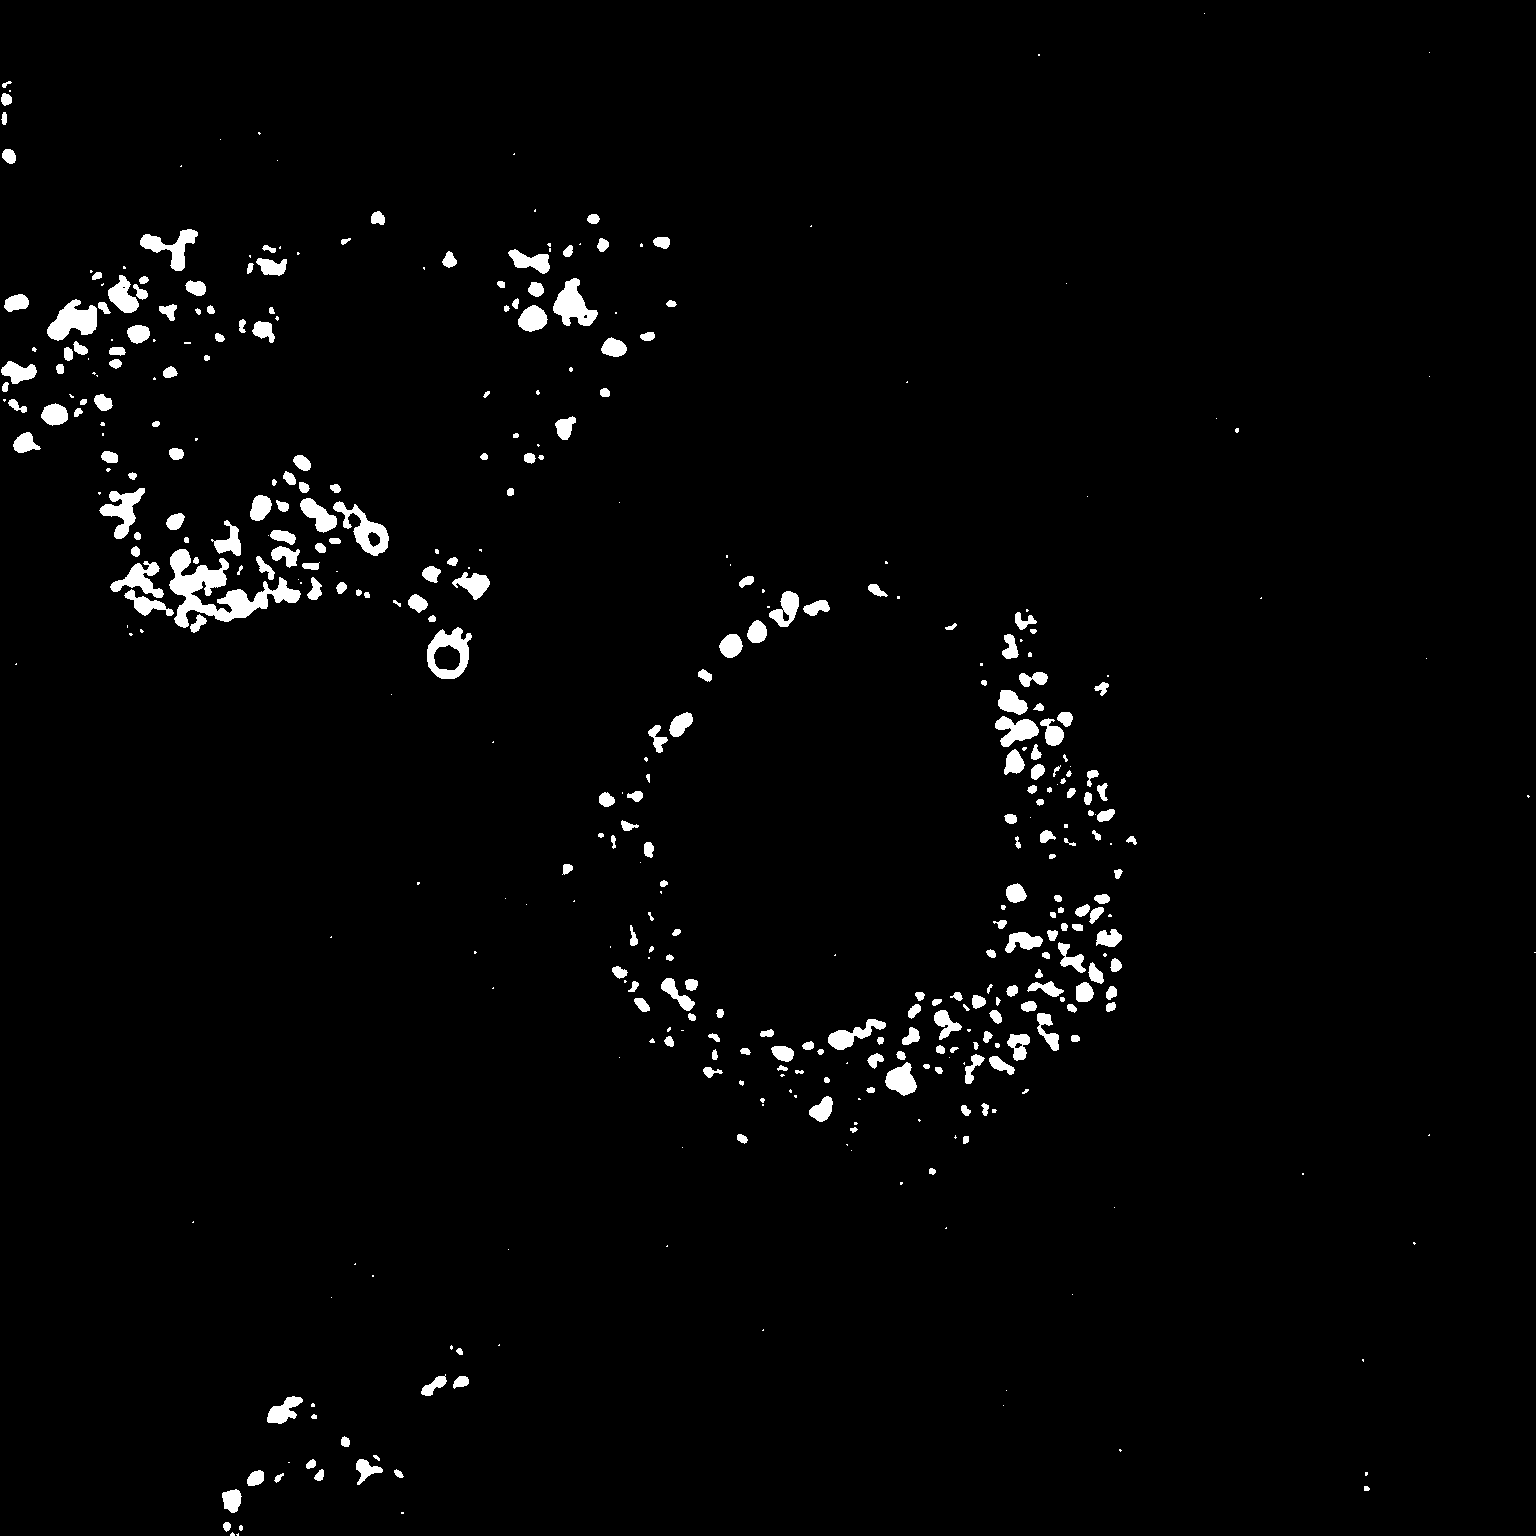
\includegraphics[width=0.2\textwidth]{figs/appendix/method_shortlisting/global_testing/Huang2_LML_4C=1.png}}
	\label{append-fig:huang2_short}
	\caption{Huang2 threshold outcomes for the shortlist sample images}
\end{figure}

\begin{figure}[ht!]
	\centering
	\subcaptionbox{Sample 1}{
\includegraphics[width=0.2\textwidth]{figs/appendix/method_shortlisting/global_testing/Intermodes_CCCP_1C=1T=0.png}}
	\subcaptionbox{Sample 2}{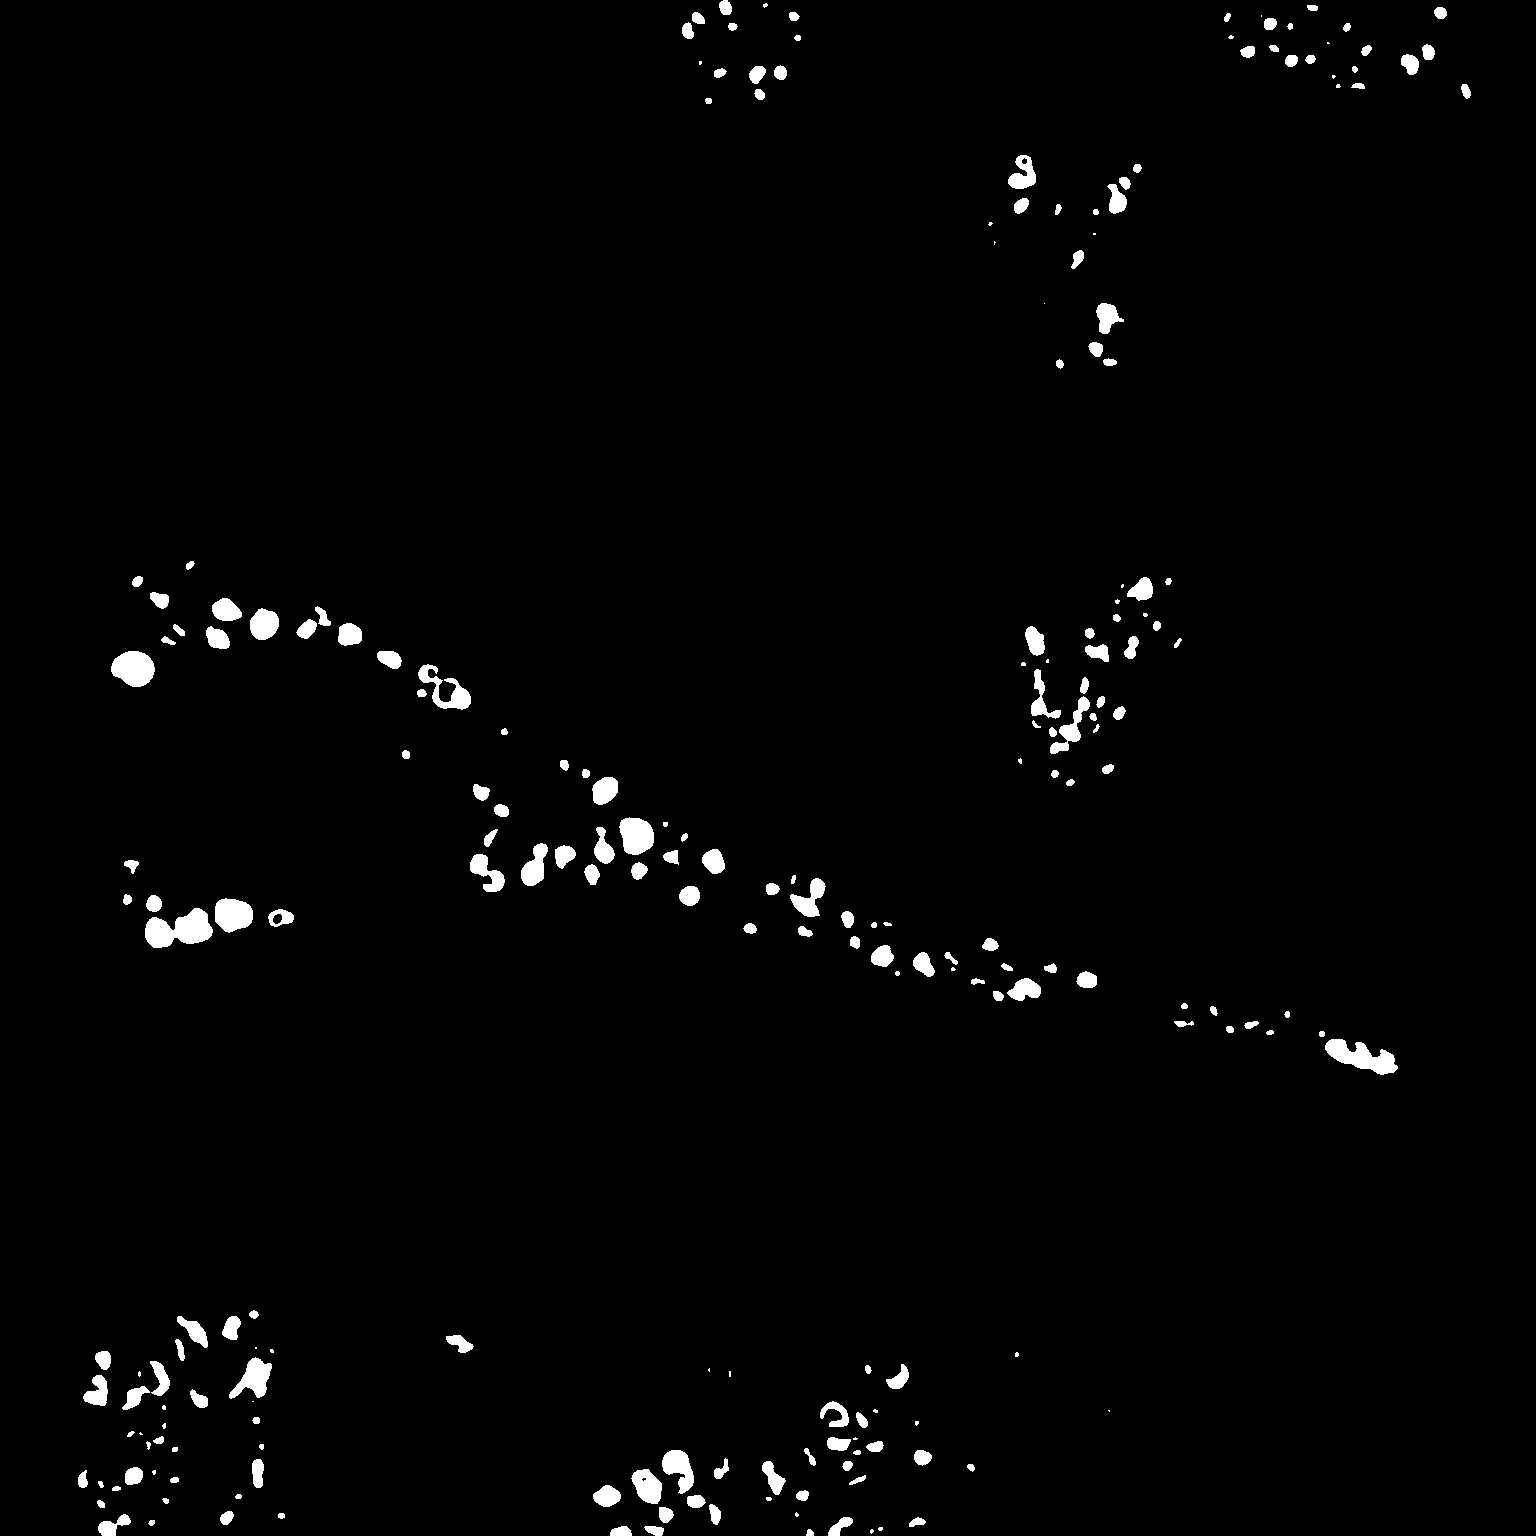
\includegraphics[width=0.2\textwidth]{figs/appendix/method_shortlisting/global_testing/Intermodes_HML_4C=0.png}}
	\subcaptionbox{Sample 3}{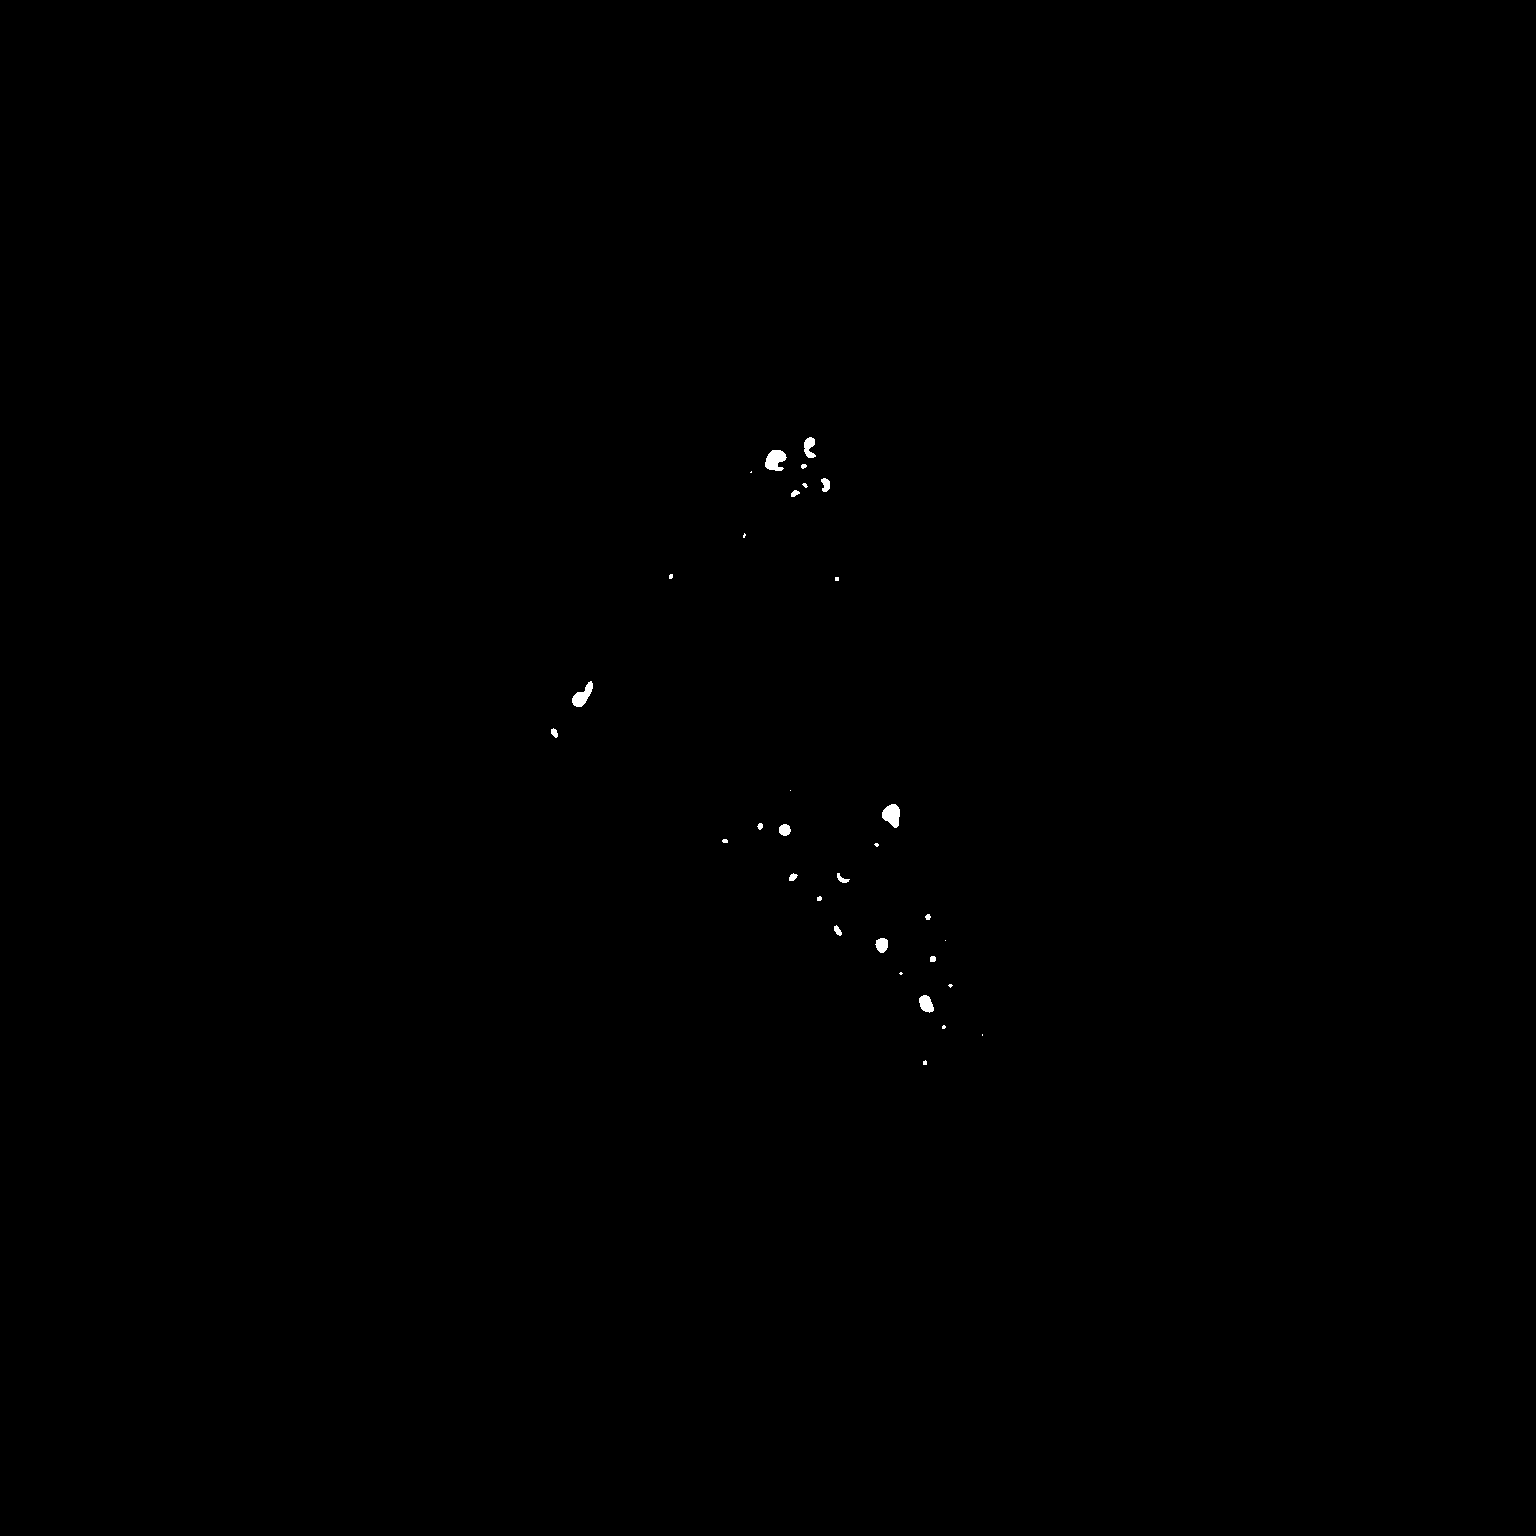
\includegraphics[width=0.2\textwidth]{figs/appendix/method_shortlisting/global_testing/Intermodes_LML_3C=0.png}}
	\subcaptionbox{Sample 4}{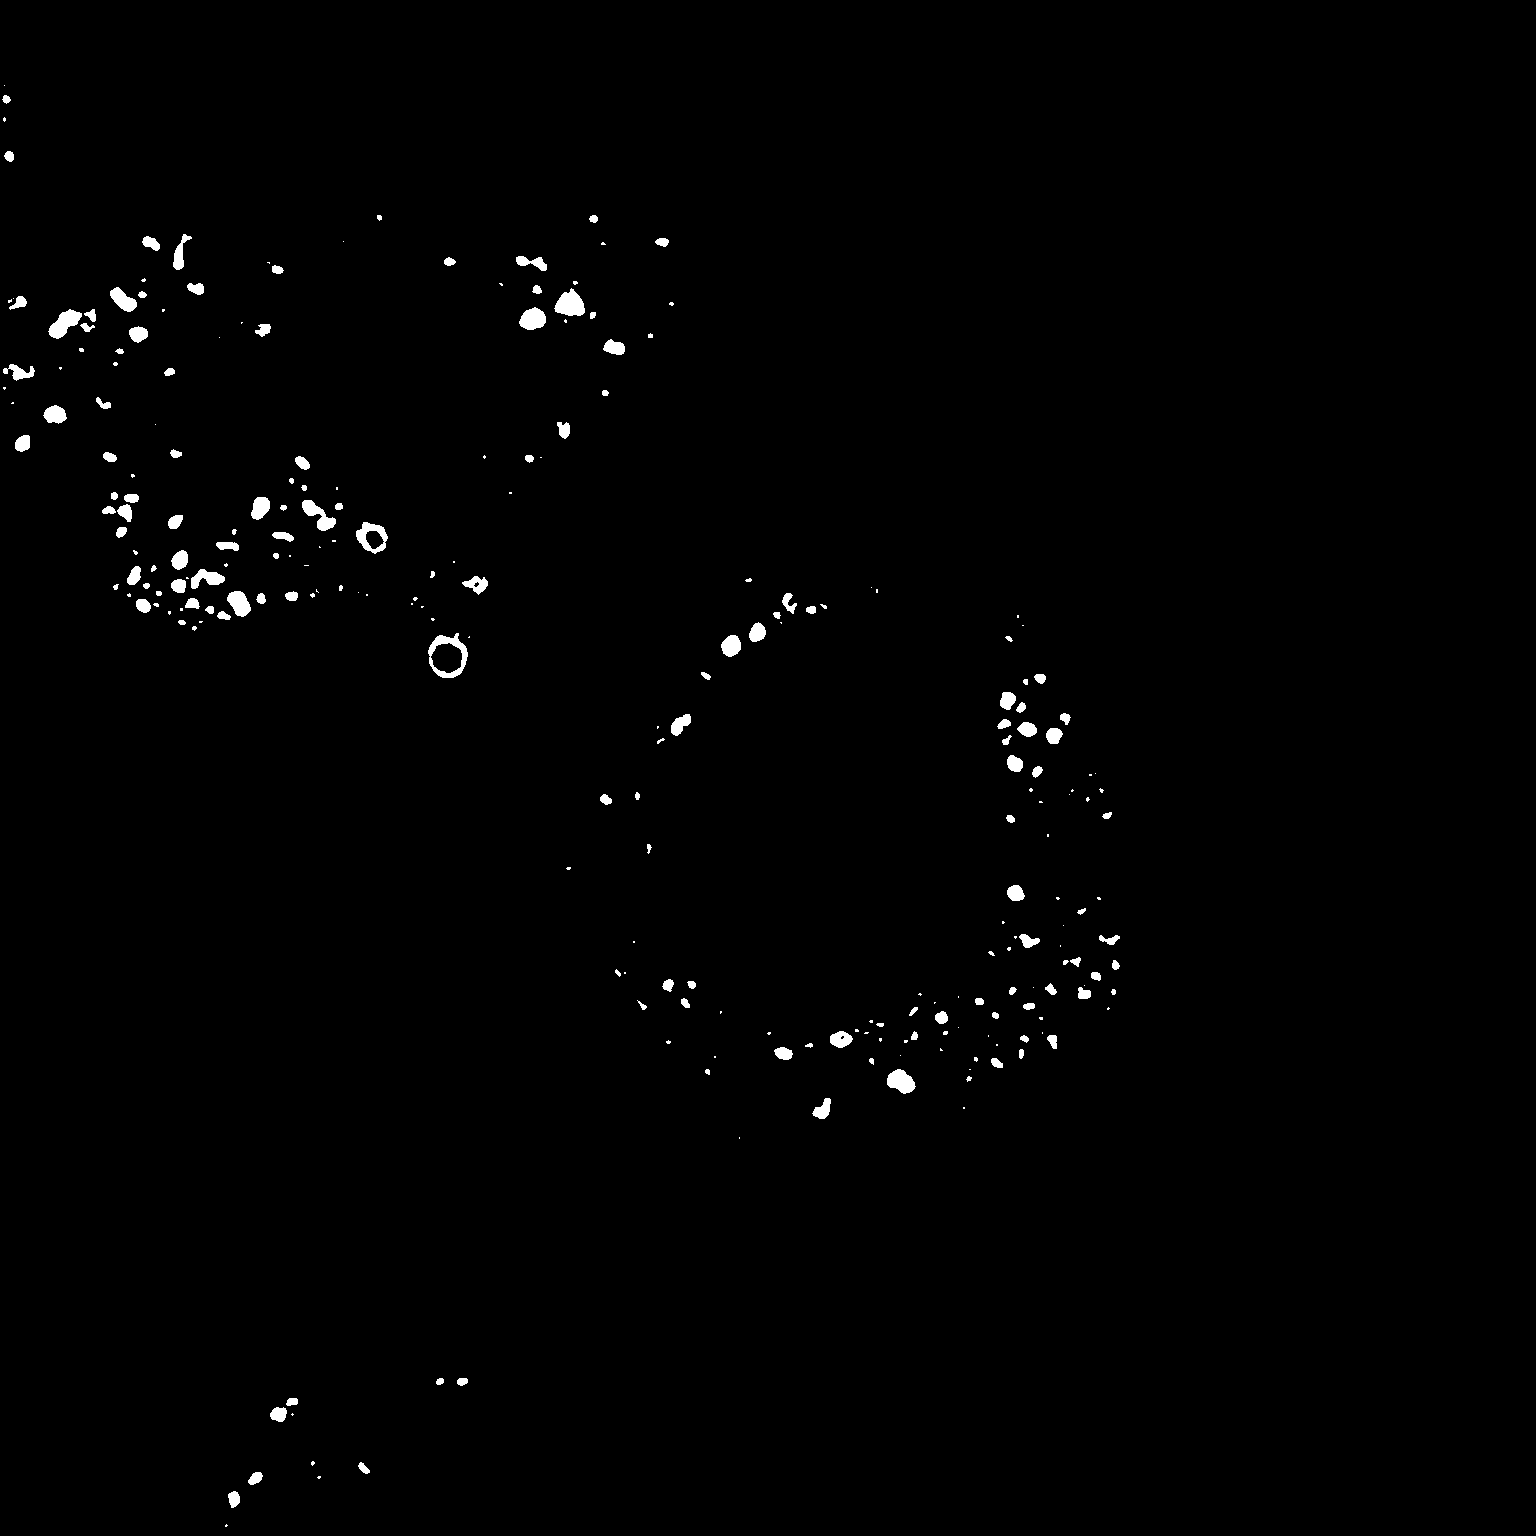
\includegraphics[width=0.2\textwidth]{figs/appendix/method_shortlisting/global_testing/Intermodes_LML_4C=1.png}}
	\label{append-fig:Intermodes_short}
	\caption{Intermodes threshold outcomes for the shortlist sample images}
\end{figure}

\begin{figure}[ht!]
	\centering
	\subcaptionbox{Sample 1}{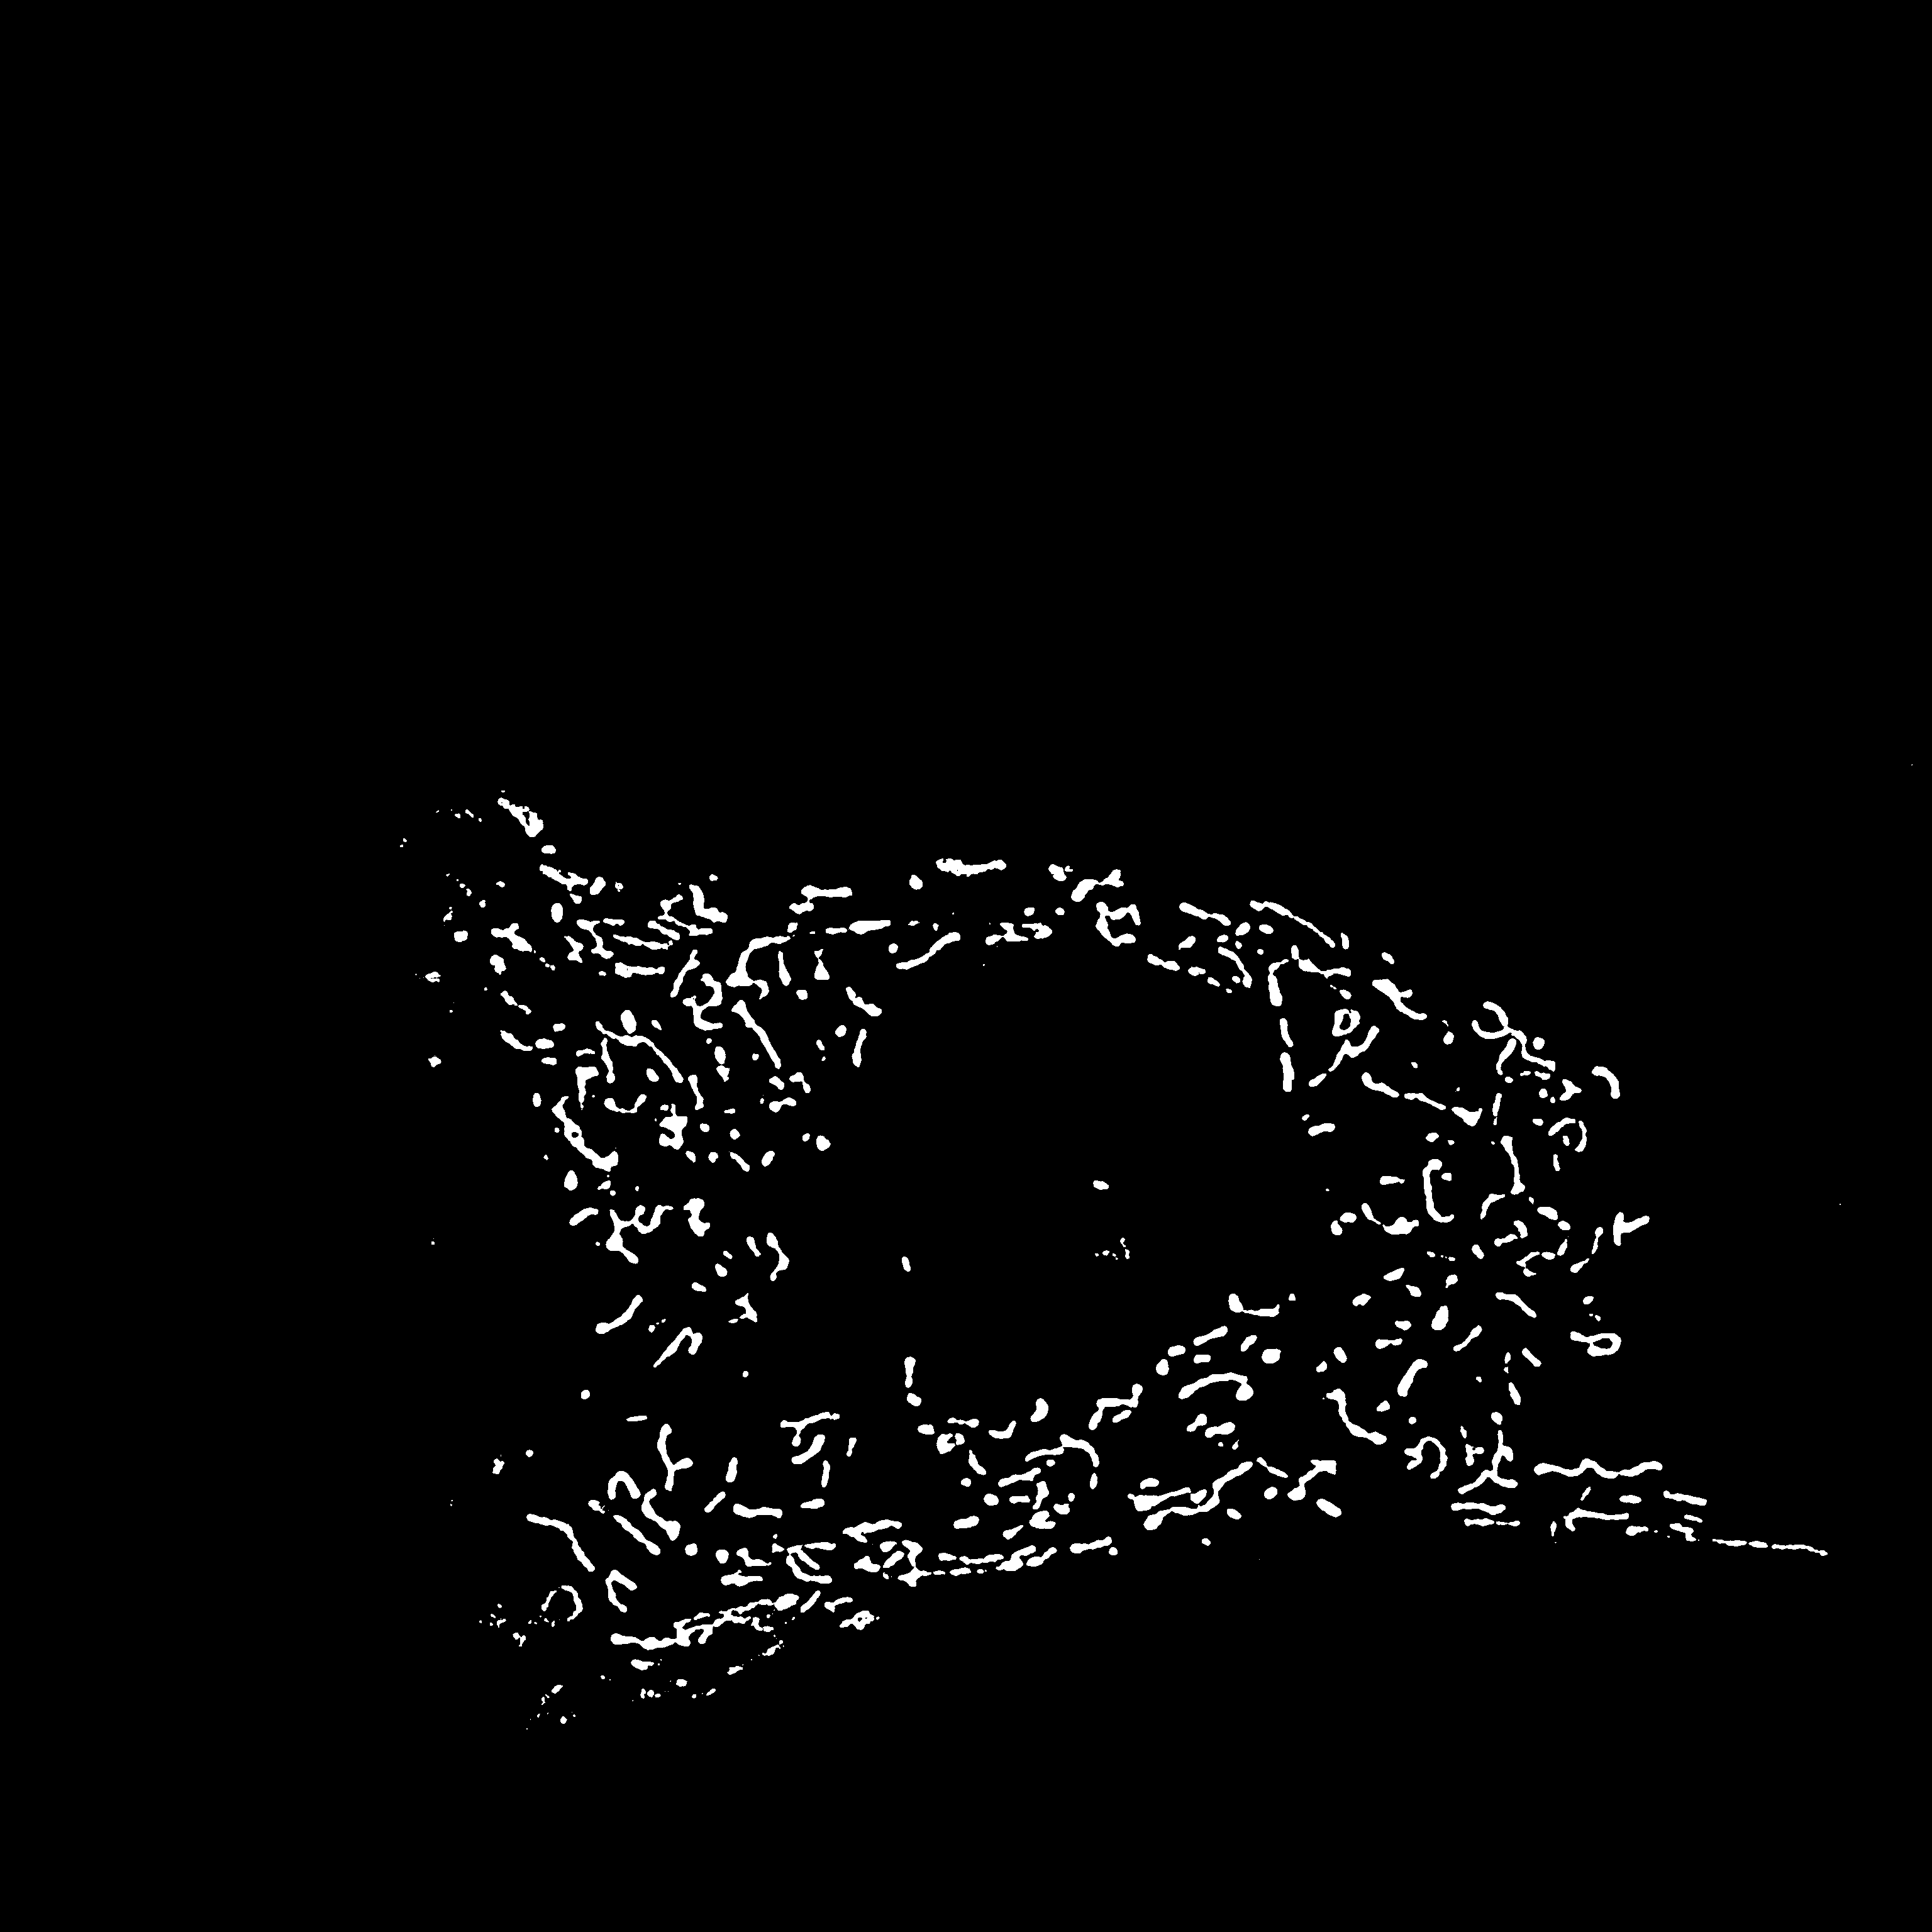
\includegraphics[width=0.2\textwidth]{figs/appendix/method_shortlisting/global_testing/IsoData_CCCP_1C=1T=0.png}}
	\subcaptionbox{Sample 2}{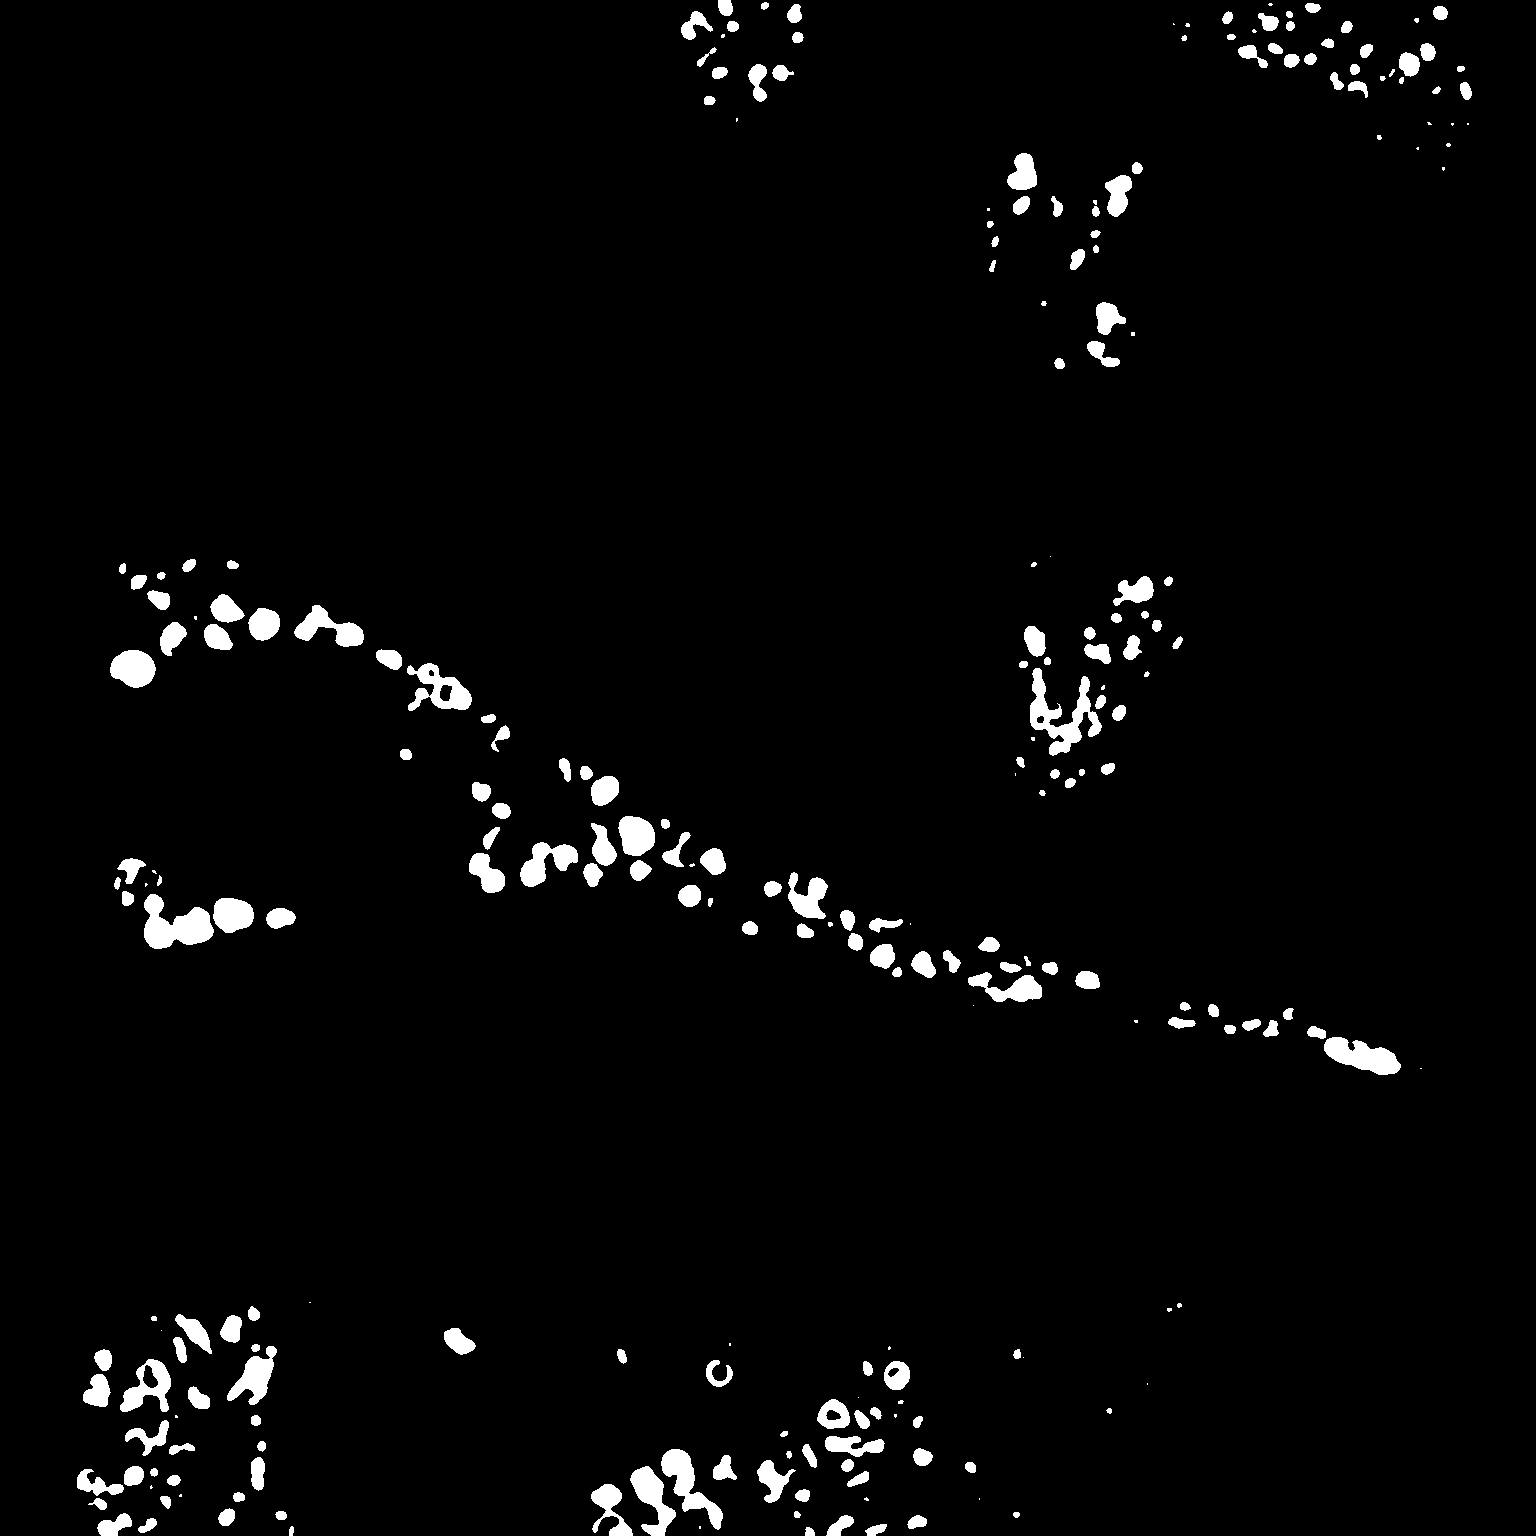
\includegraphics[width=0.2\textwidth]{figs/appendix/method_shortlisting/global_testing/IsoData_HML_4C=0.png}}
	\subcaptionbox{Sample 3}{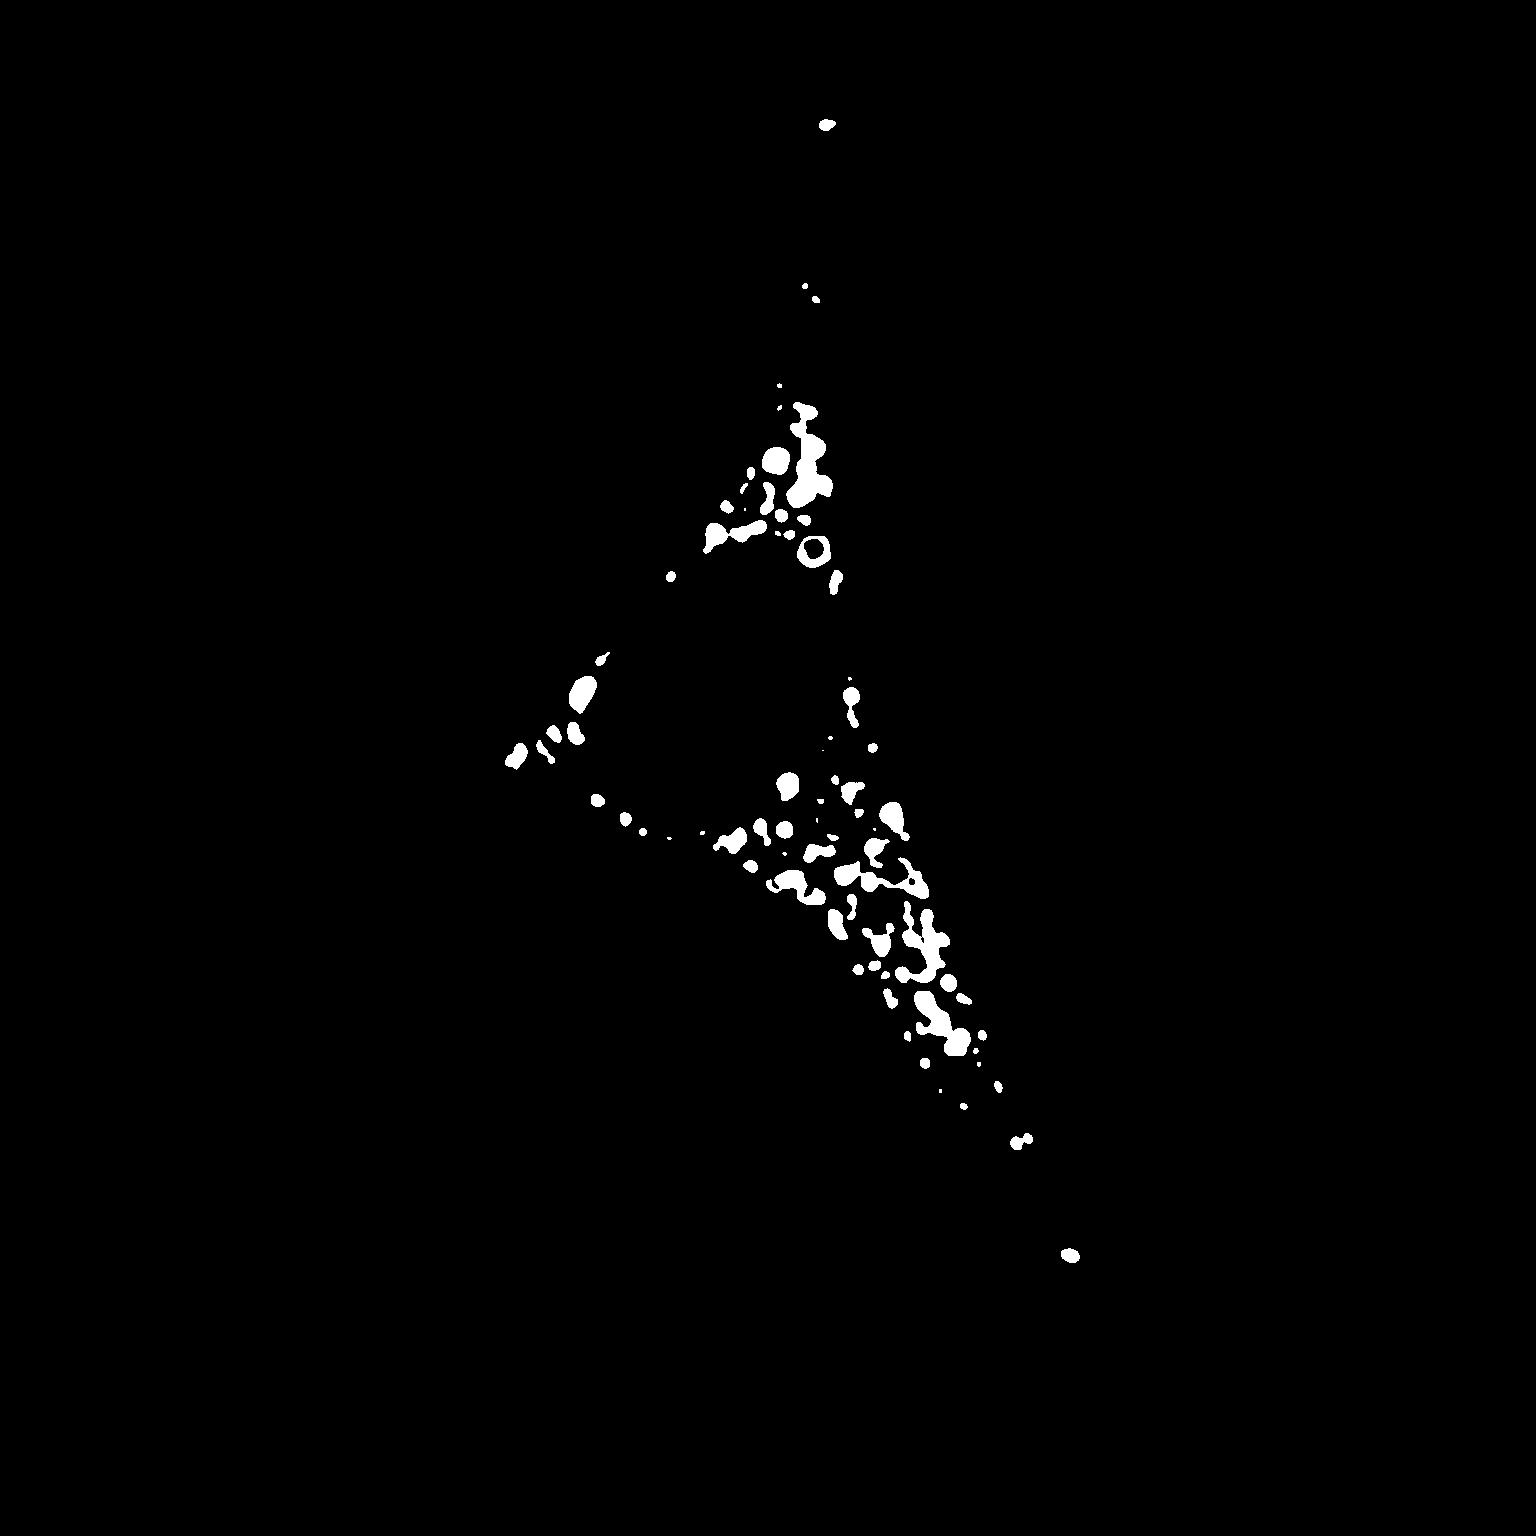
\includegraphics[width=0.2\textwidth]{figs/appendix/method_shortlisting/global_testing/IsoData_LML_3C=0.png}}
	\subcaptionbox{Sample 4}{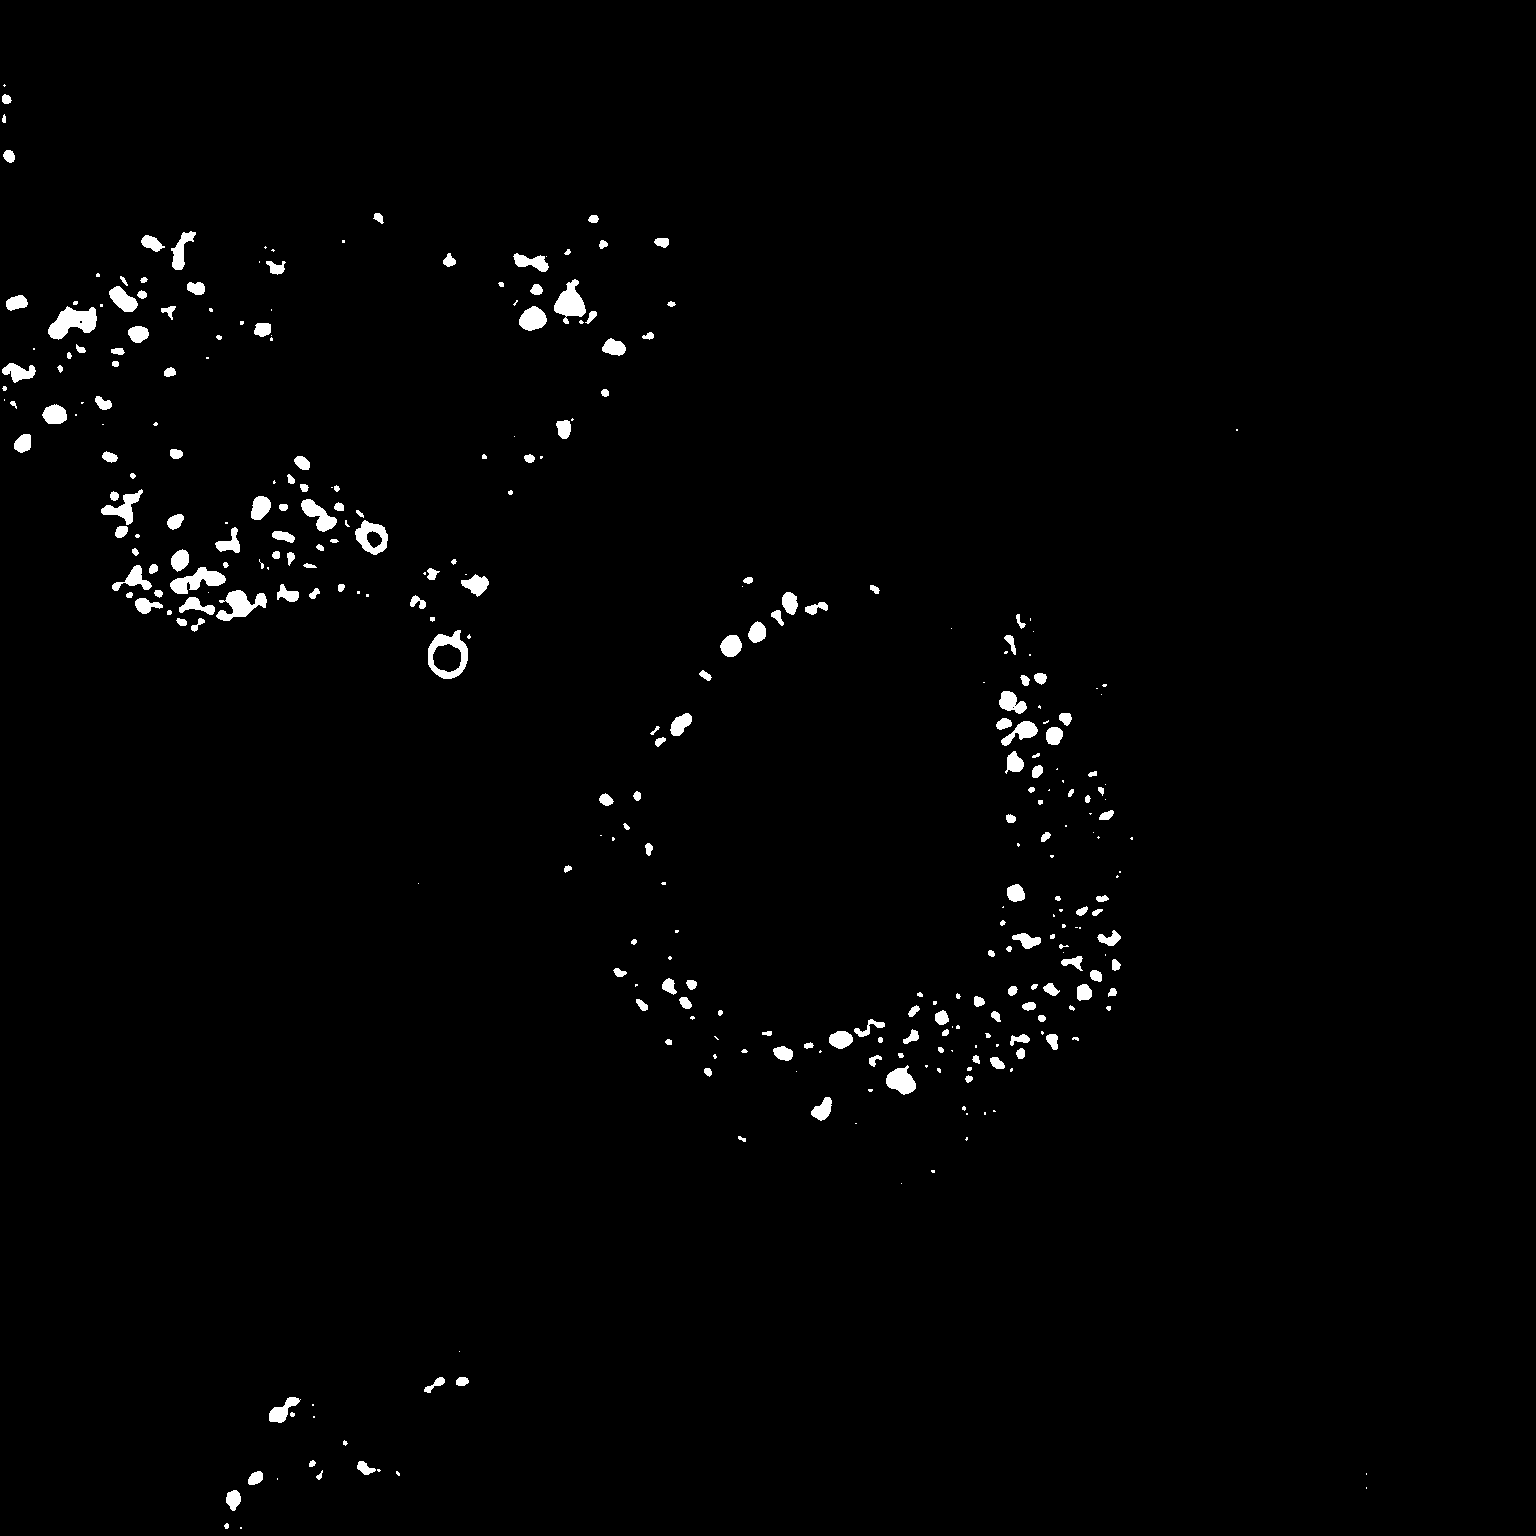
\includegraphics[width=0.2\textwidth]{figs/appendix/method_shortlisting/global_testing/IsoData_LML_4C=1.png}}
	\label{append-fig:IsoData_short}
	\caption{IsoData threshold outcomes for the shortlist sample images}
\end{figure}

\begin{figure}[ht!]
	\centering
	\subcaptionbox{Sample 1}{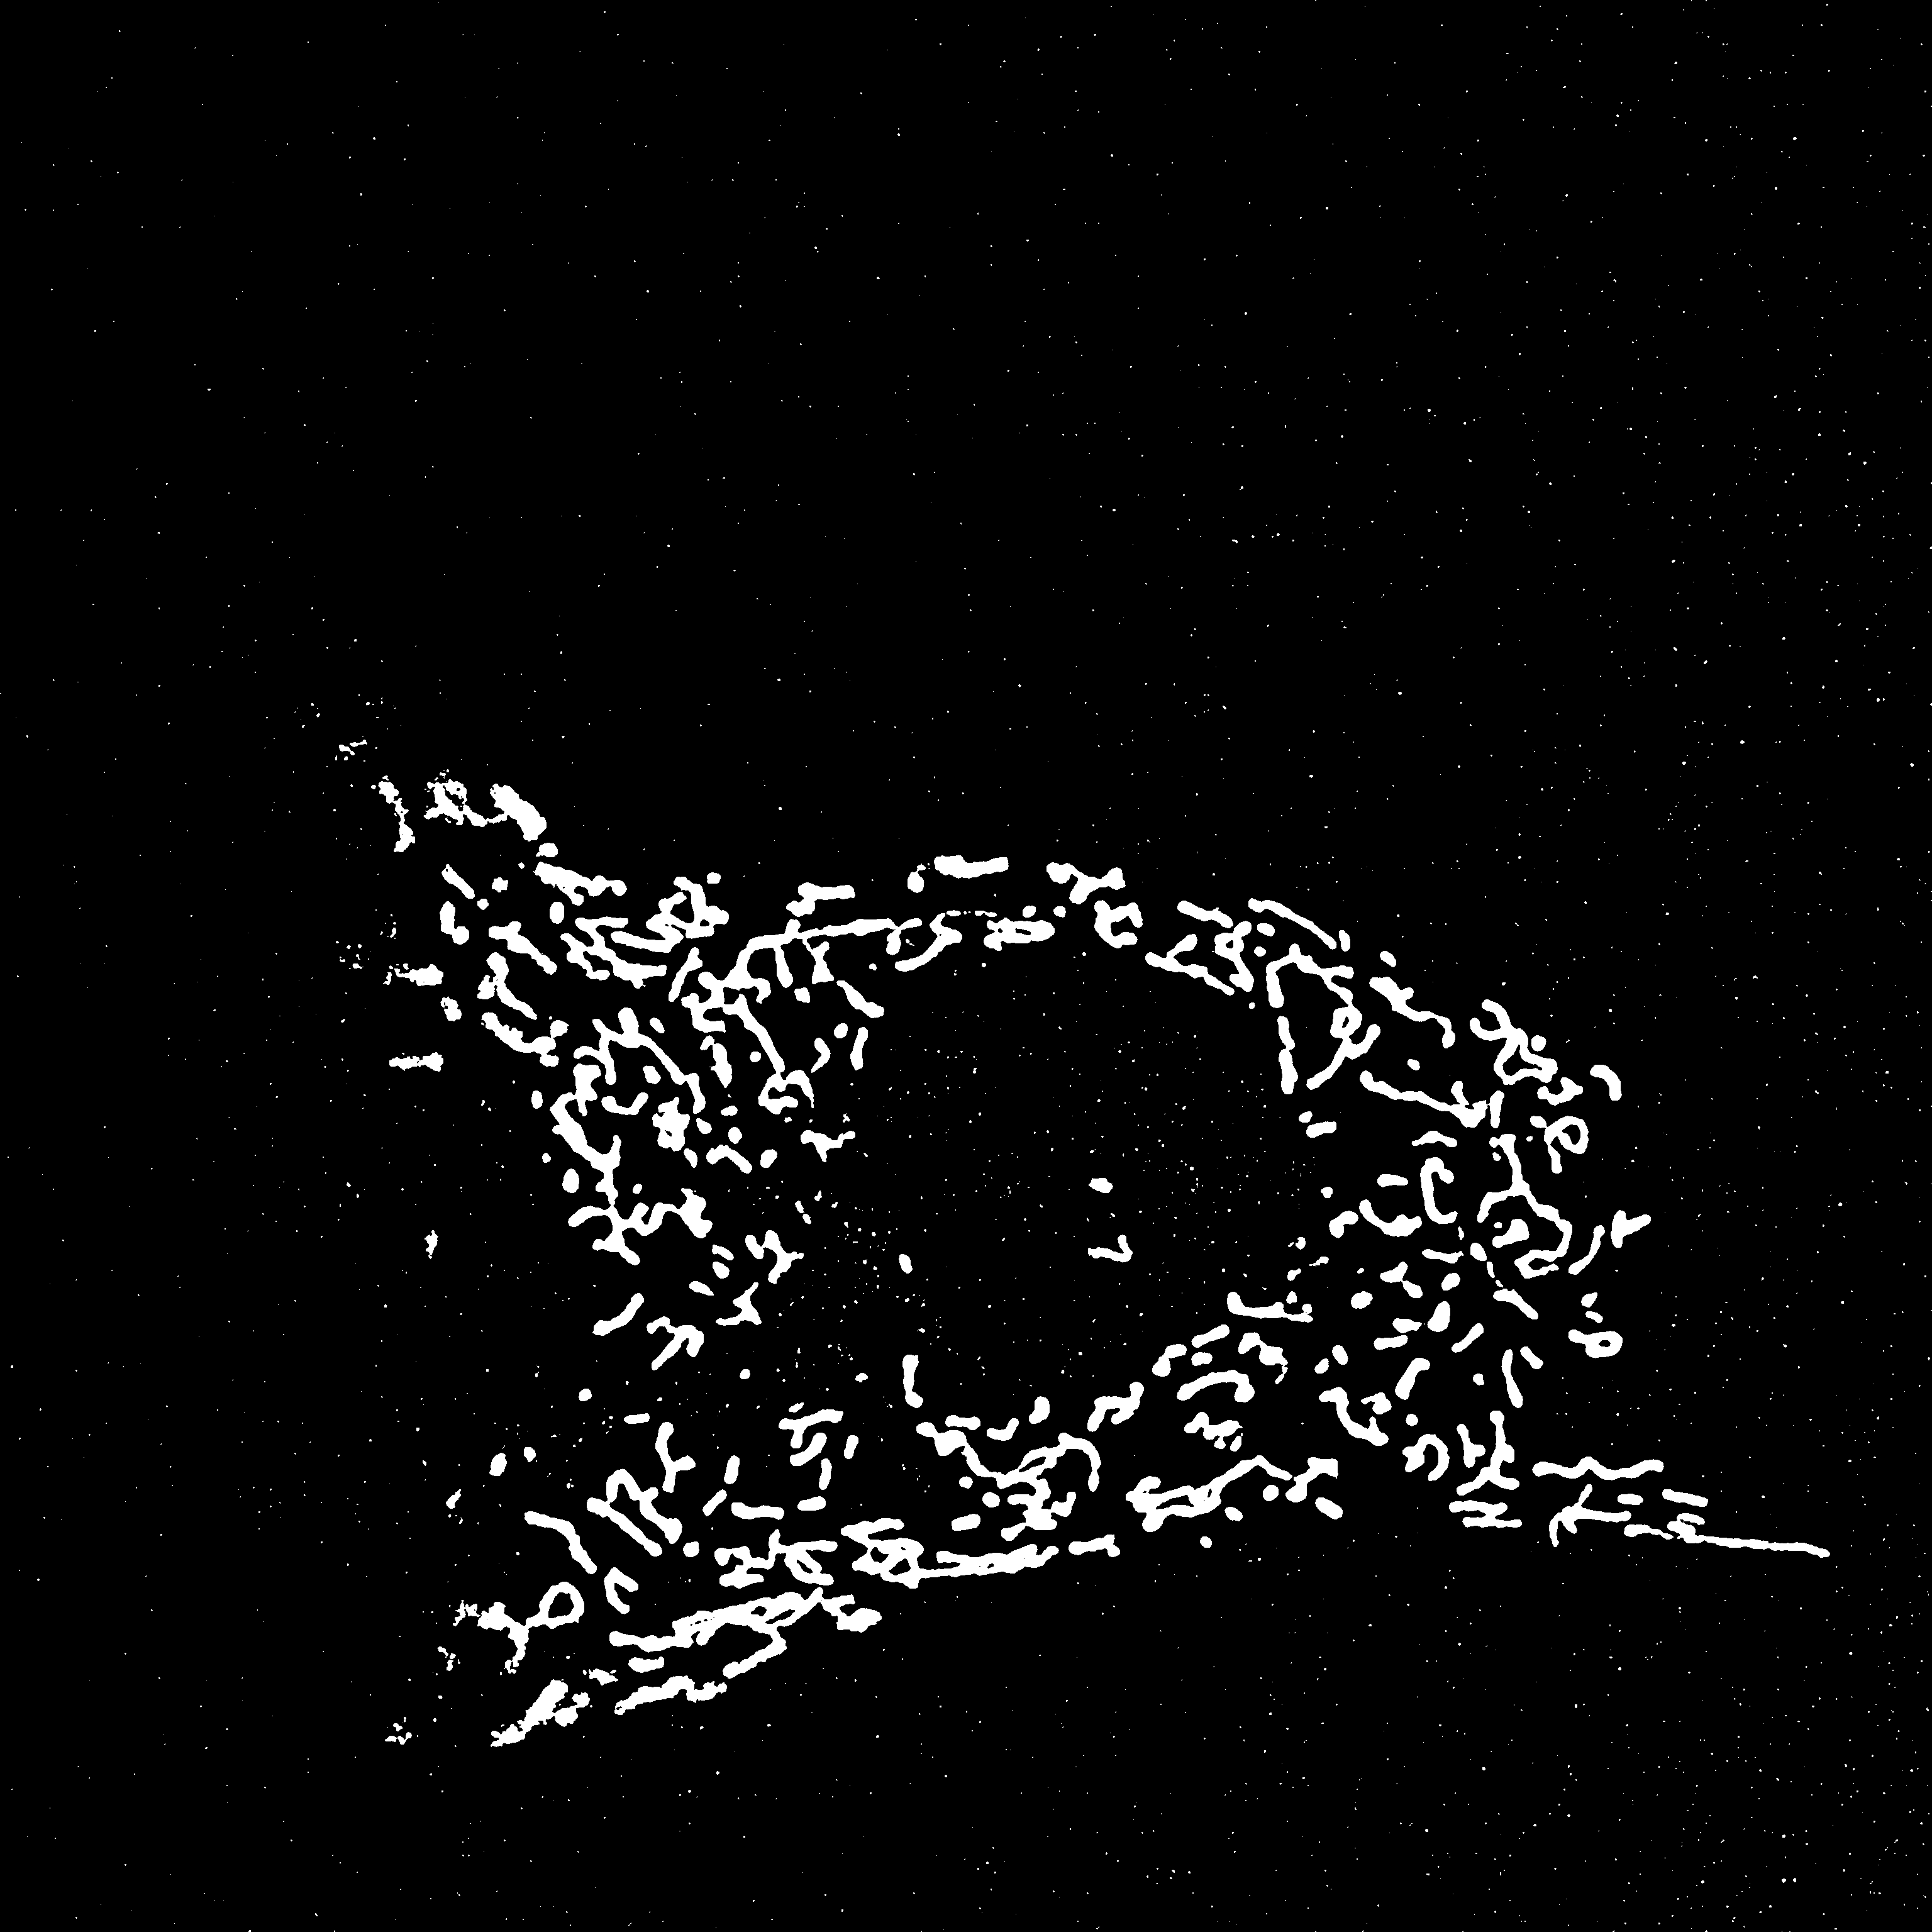
\includegraphics[width=0.2\textwidth]{figs/appendix/method_shortlisting/global_testing/Li_CCCP_1C=1T=0.png}}
	\subcaptionbox{Sample 2}{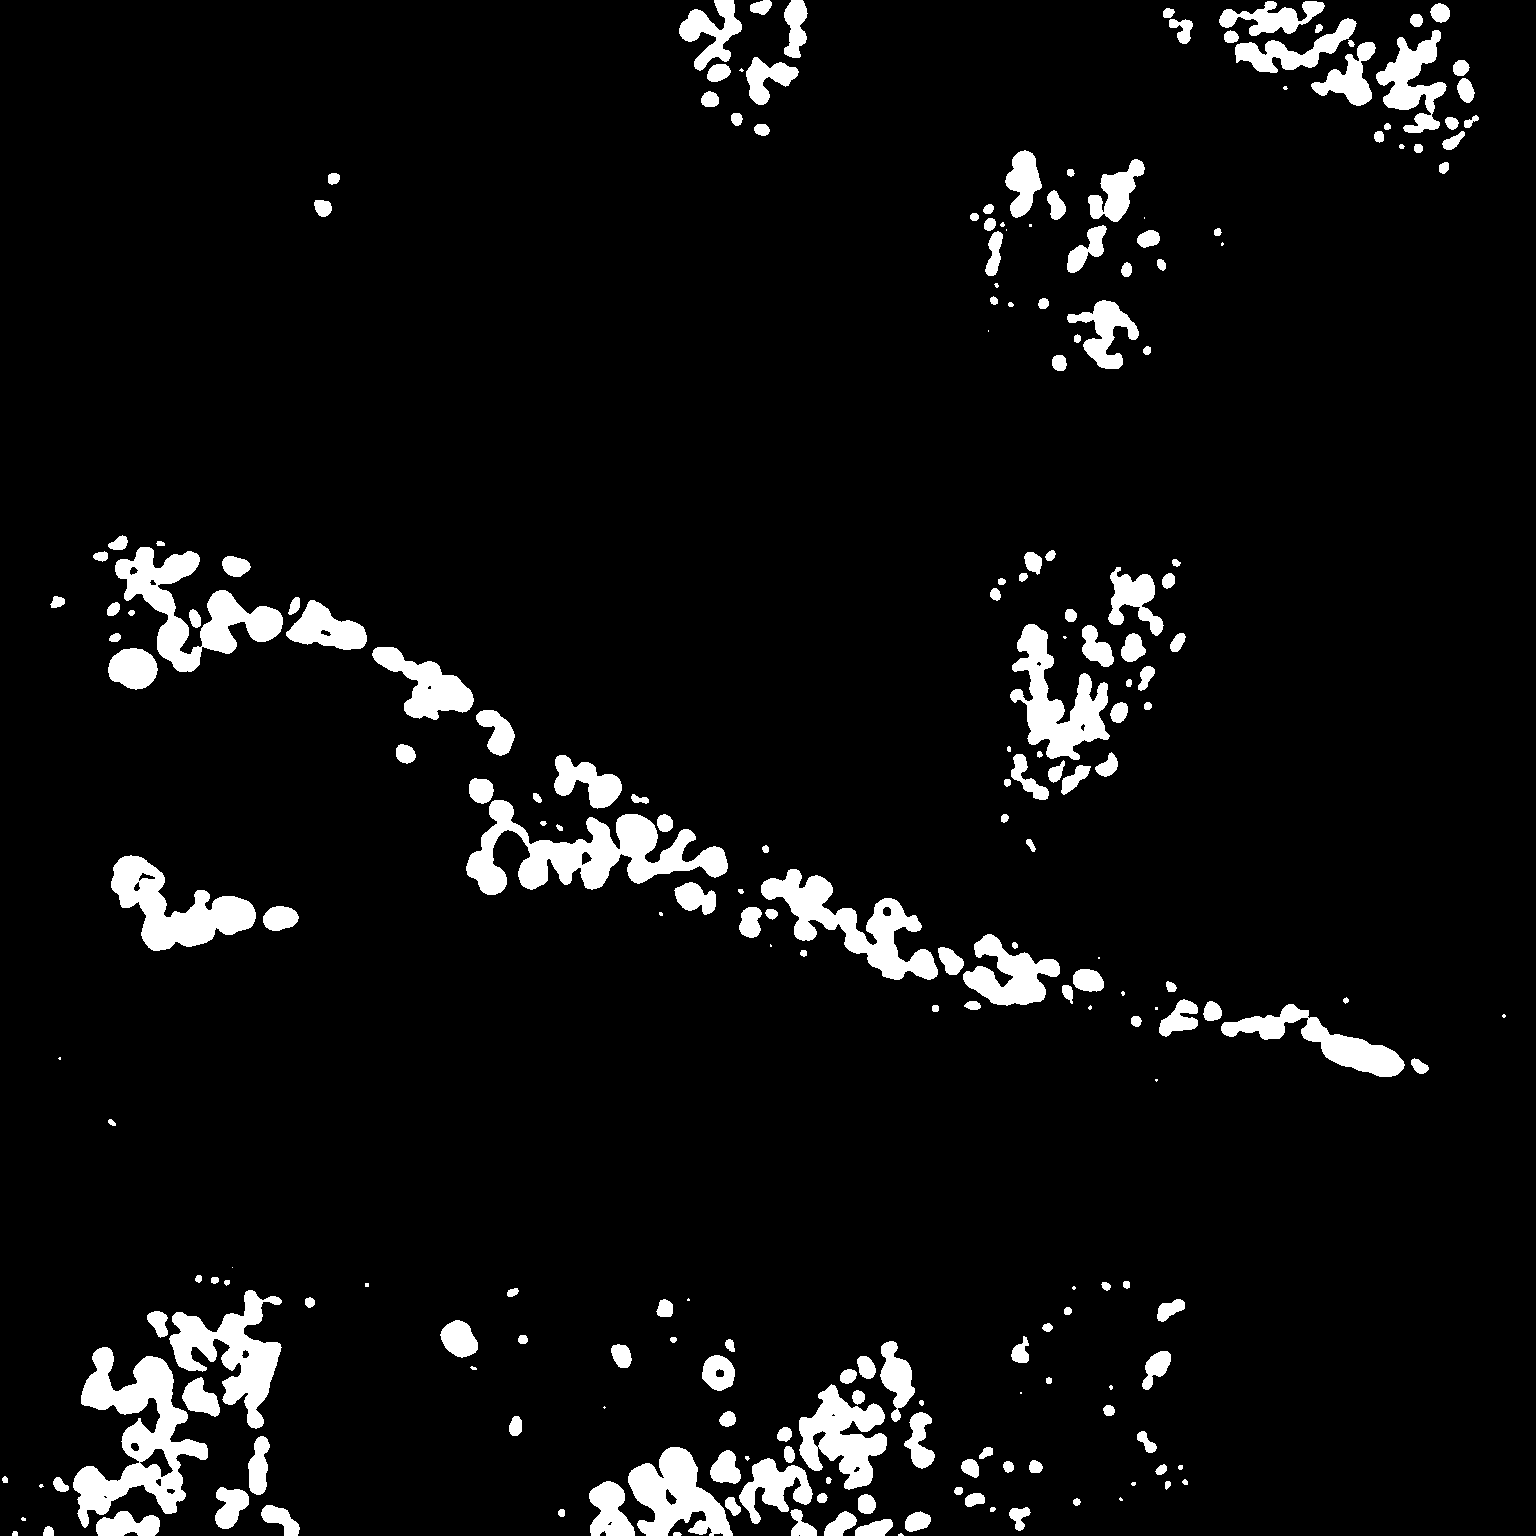
\includegraphics[width=0.2\textwidth]{figs/appendix/method_shortlisting/global_testing/Li_HML_4C=0.png}}
	\subcaptionbox{Sample 3}{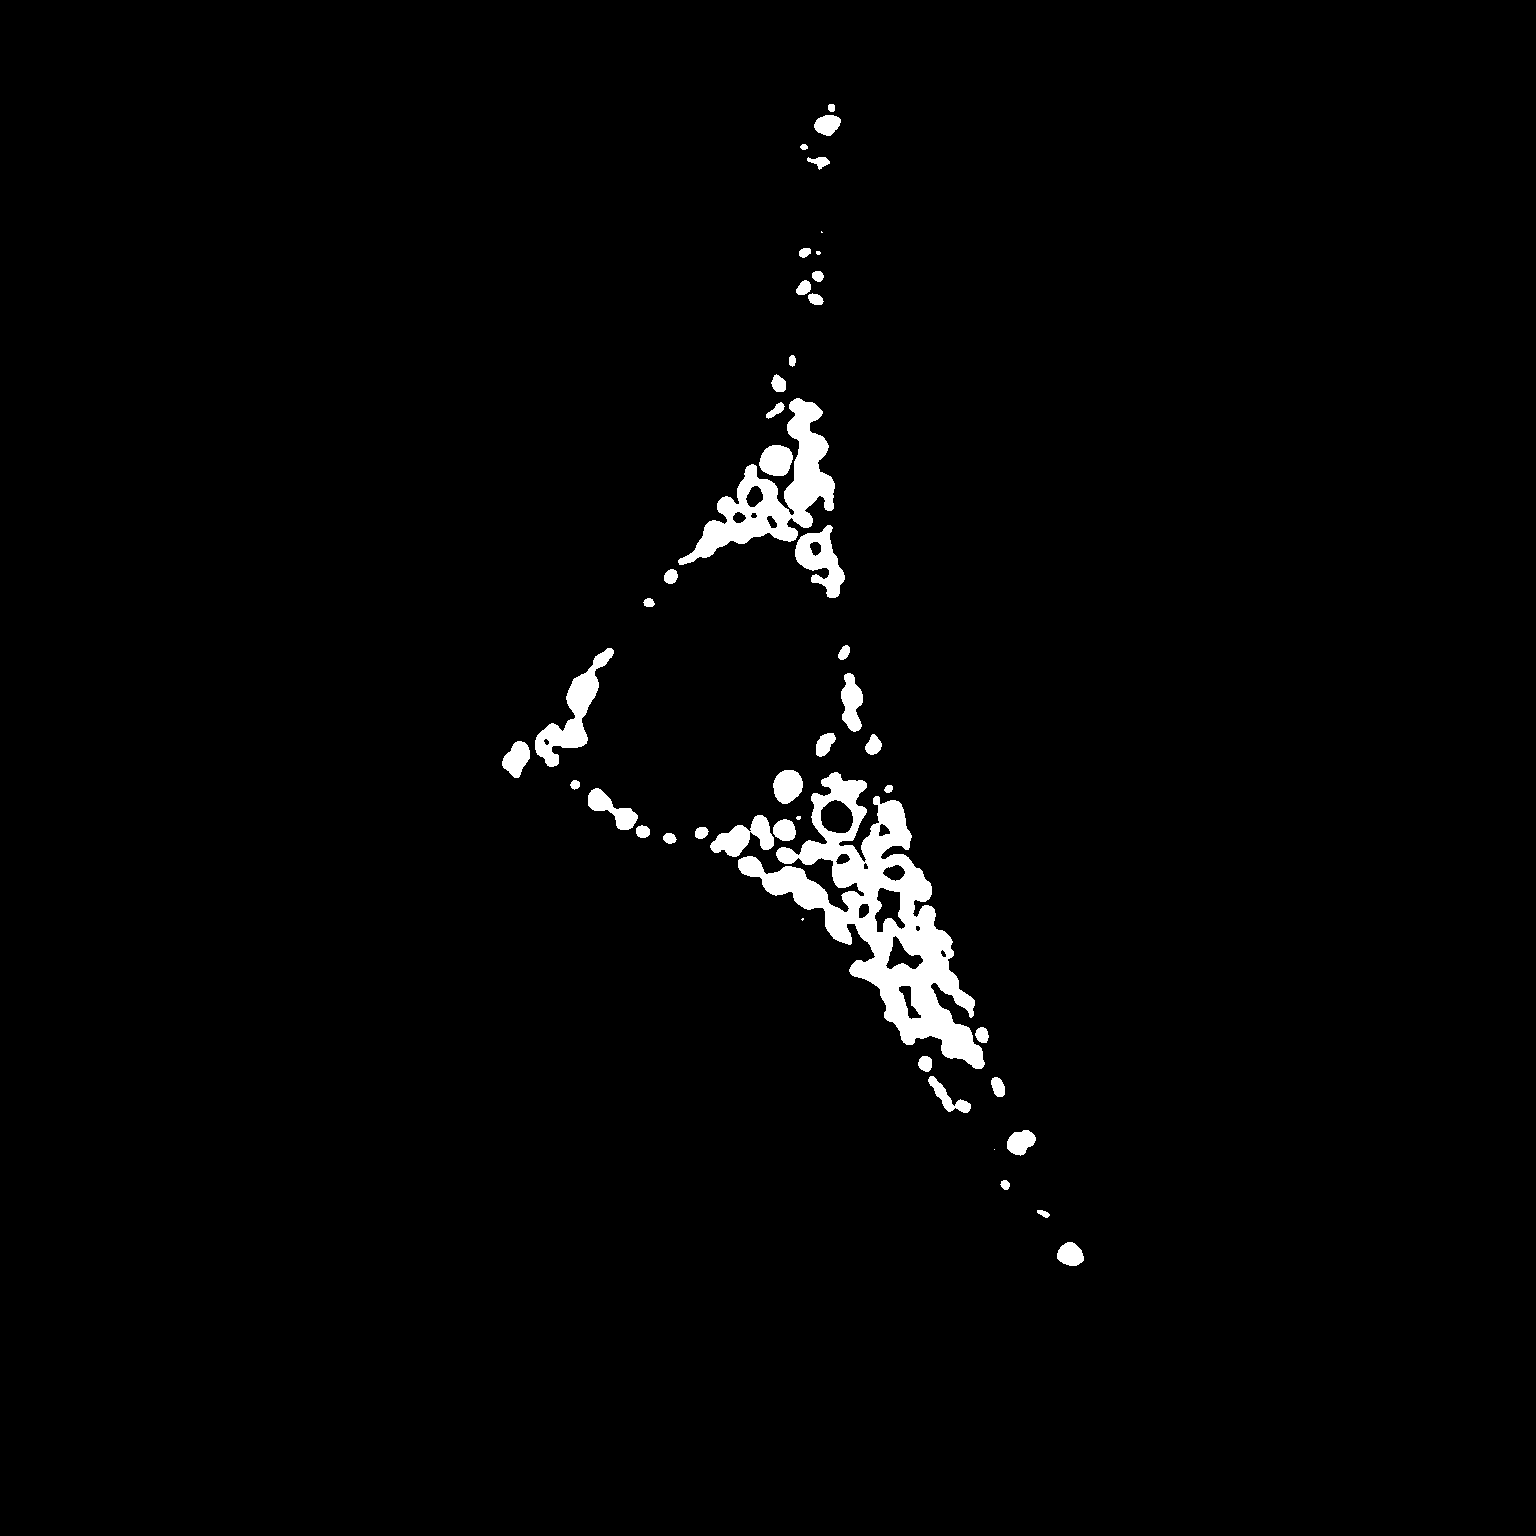
\includegraphics[width=0.2\textwidth]{figs/appendix/method_shortlisting/global_testing/Li_LML_3C=0.png}}
	\subcaptionbox{Sample 4}{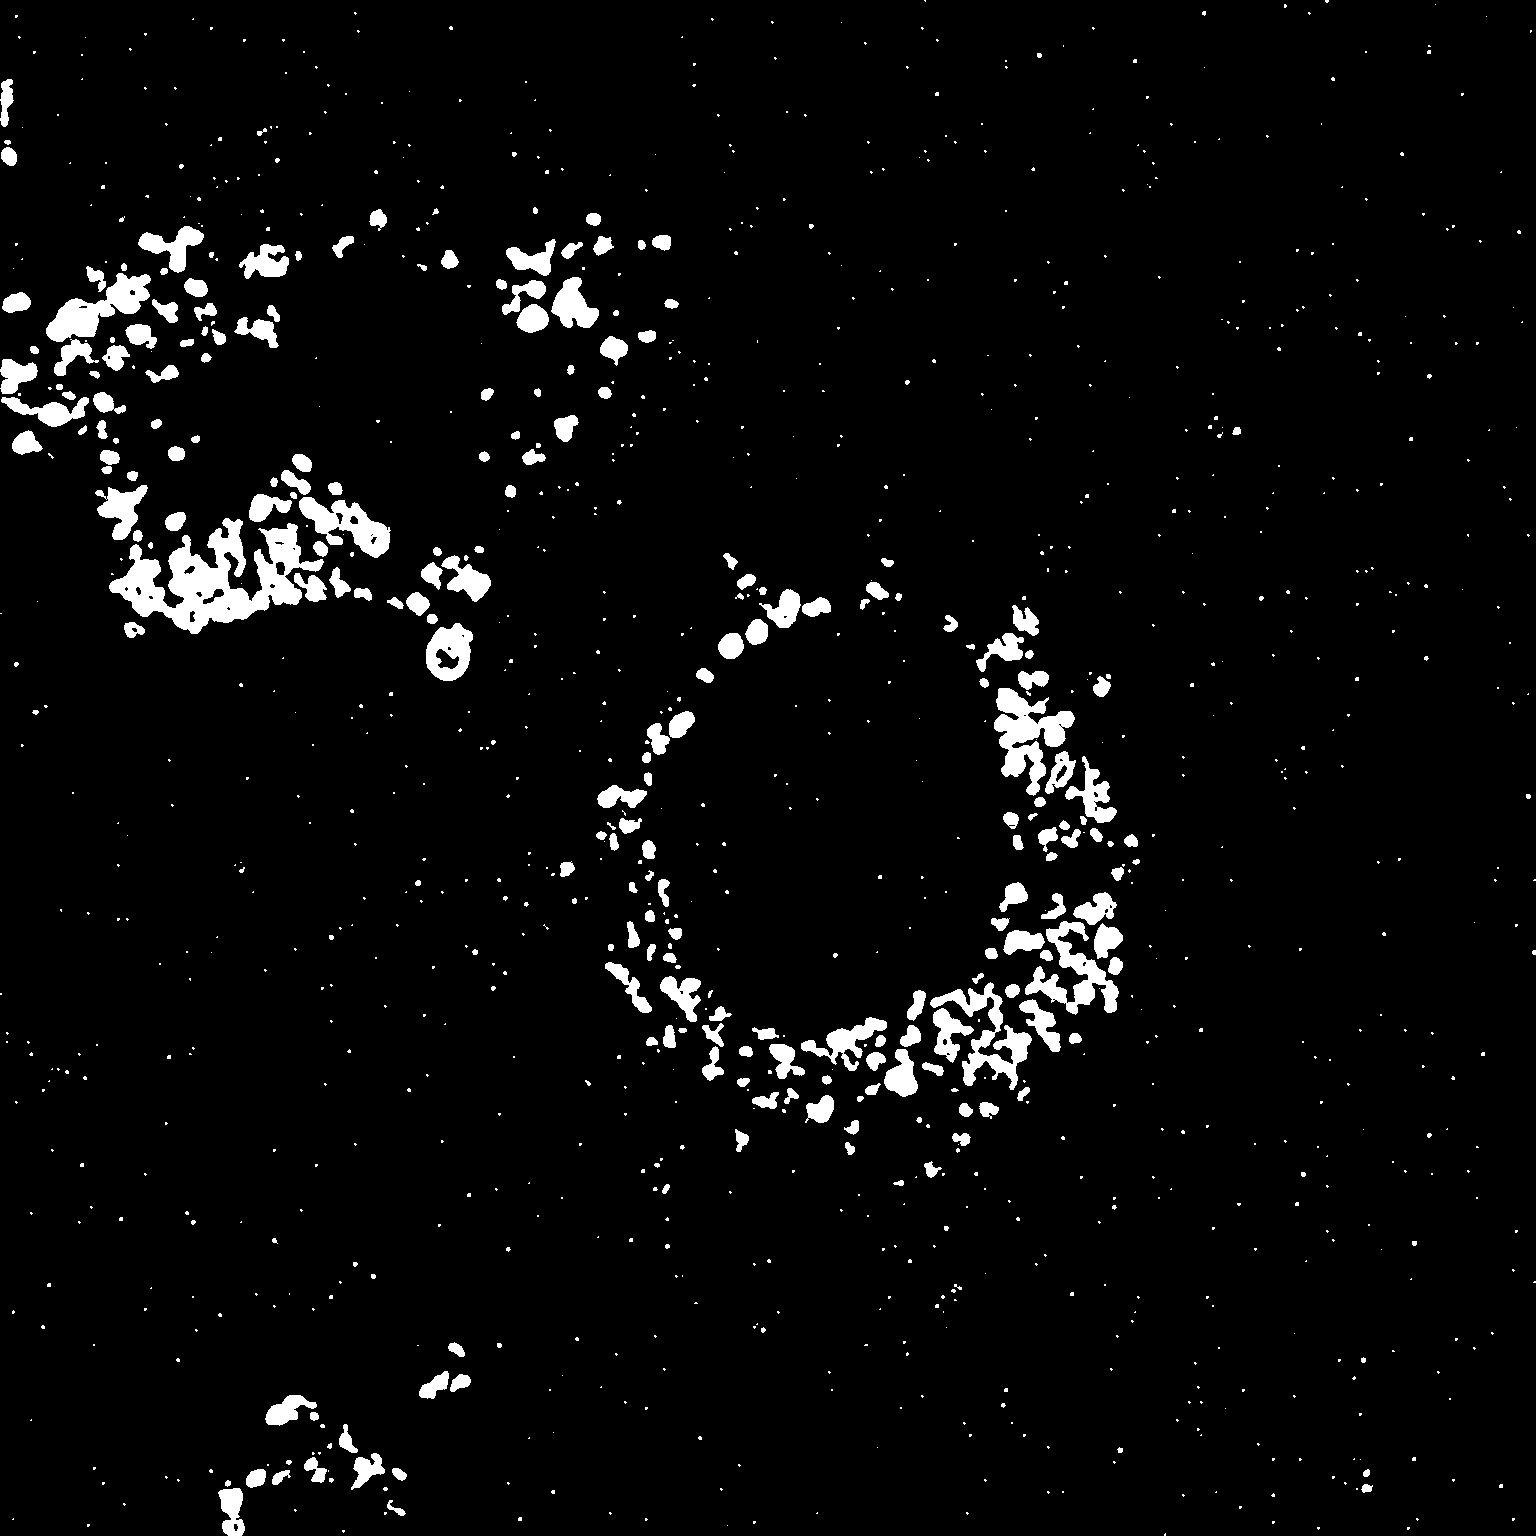
\includegraphics[width=0.2\textwidth]{figs/appendix/method_shortlisting/global_testing/Li_LML_4C=1.png}}
	\label{append-fig:li_short}
	\caption{Li threshold outcomes for the shortlist sample images}
\end{figure}

\begin{figure}[ht!]
	\centering
	\subcaptionbox{Sample 1}{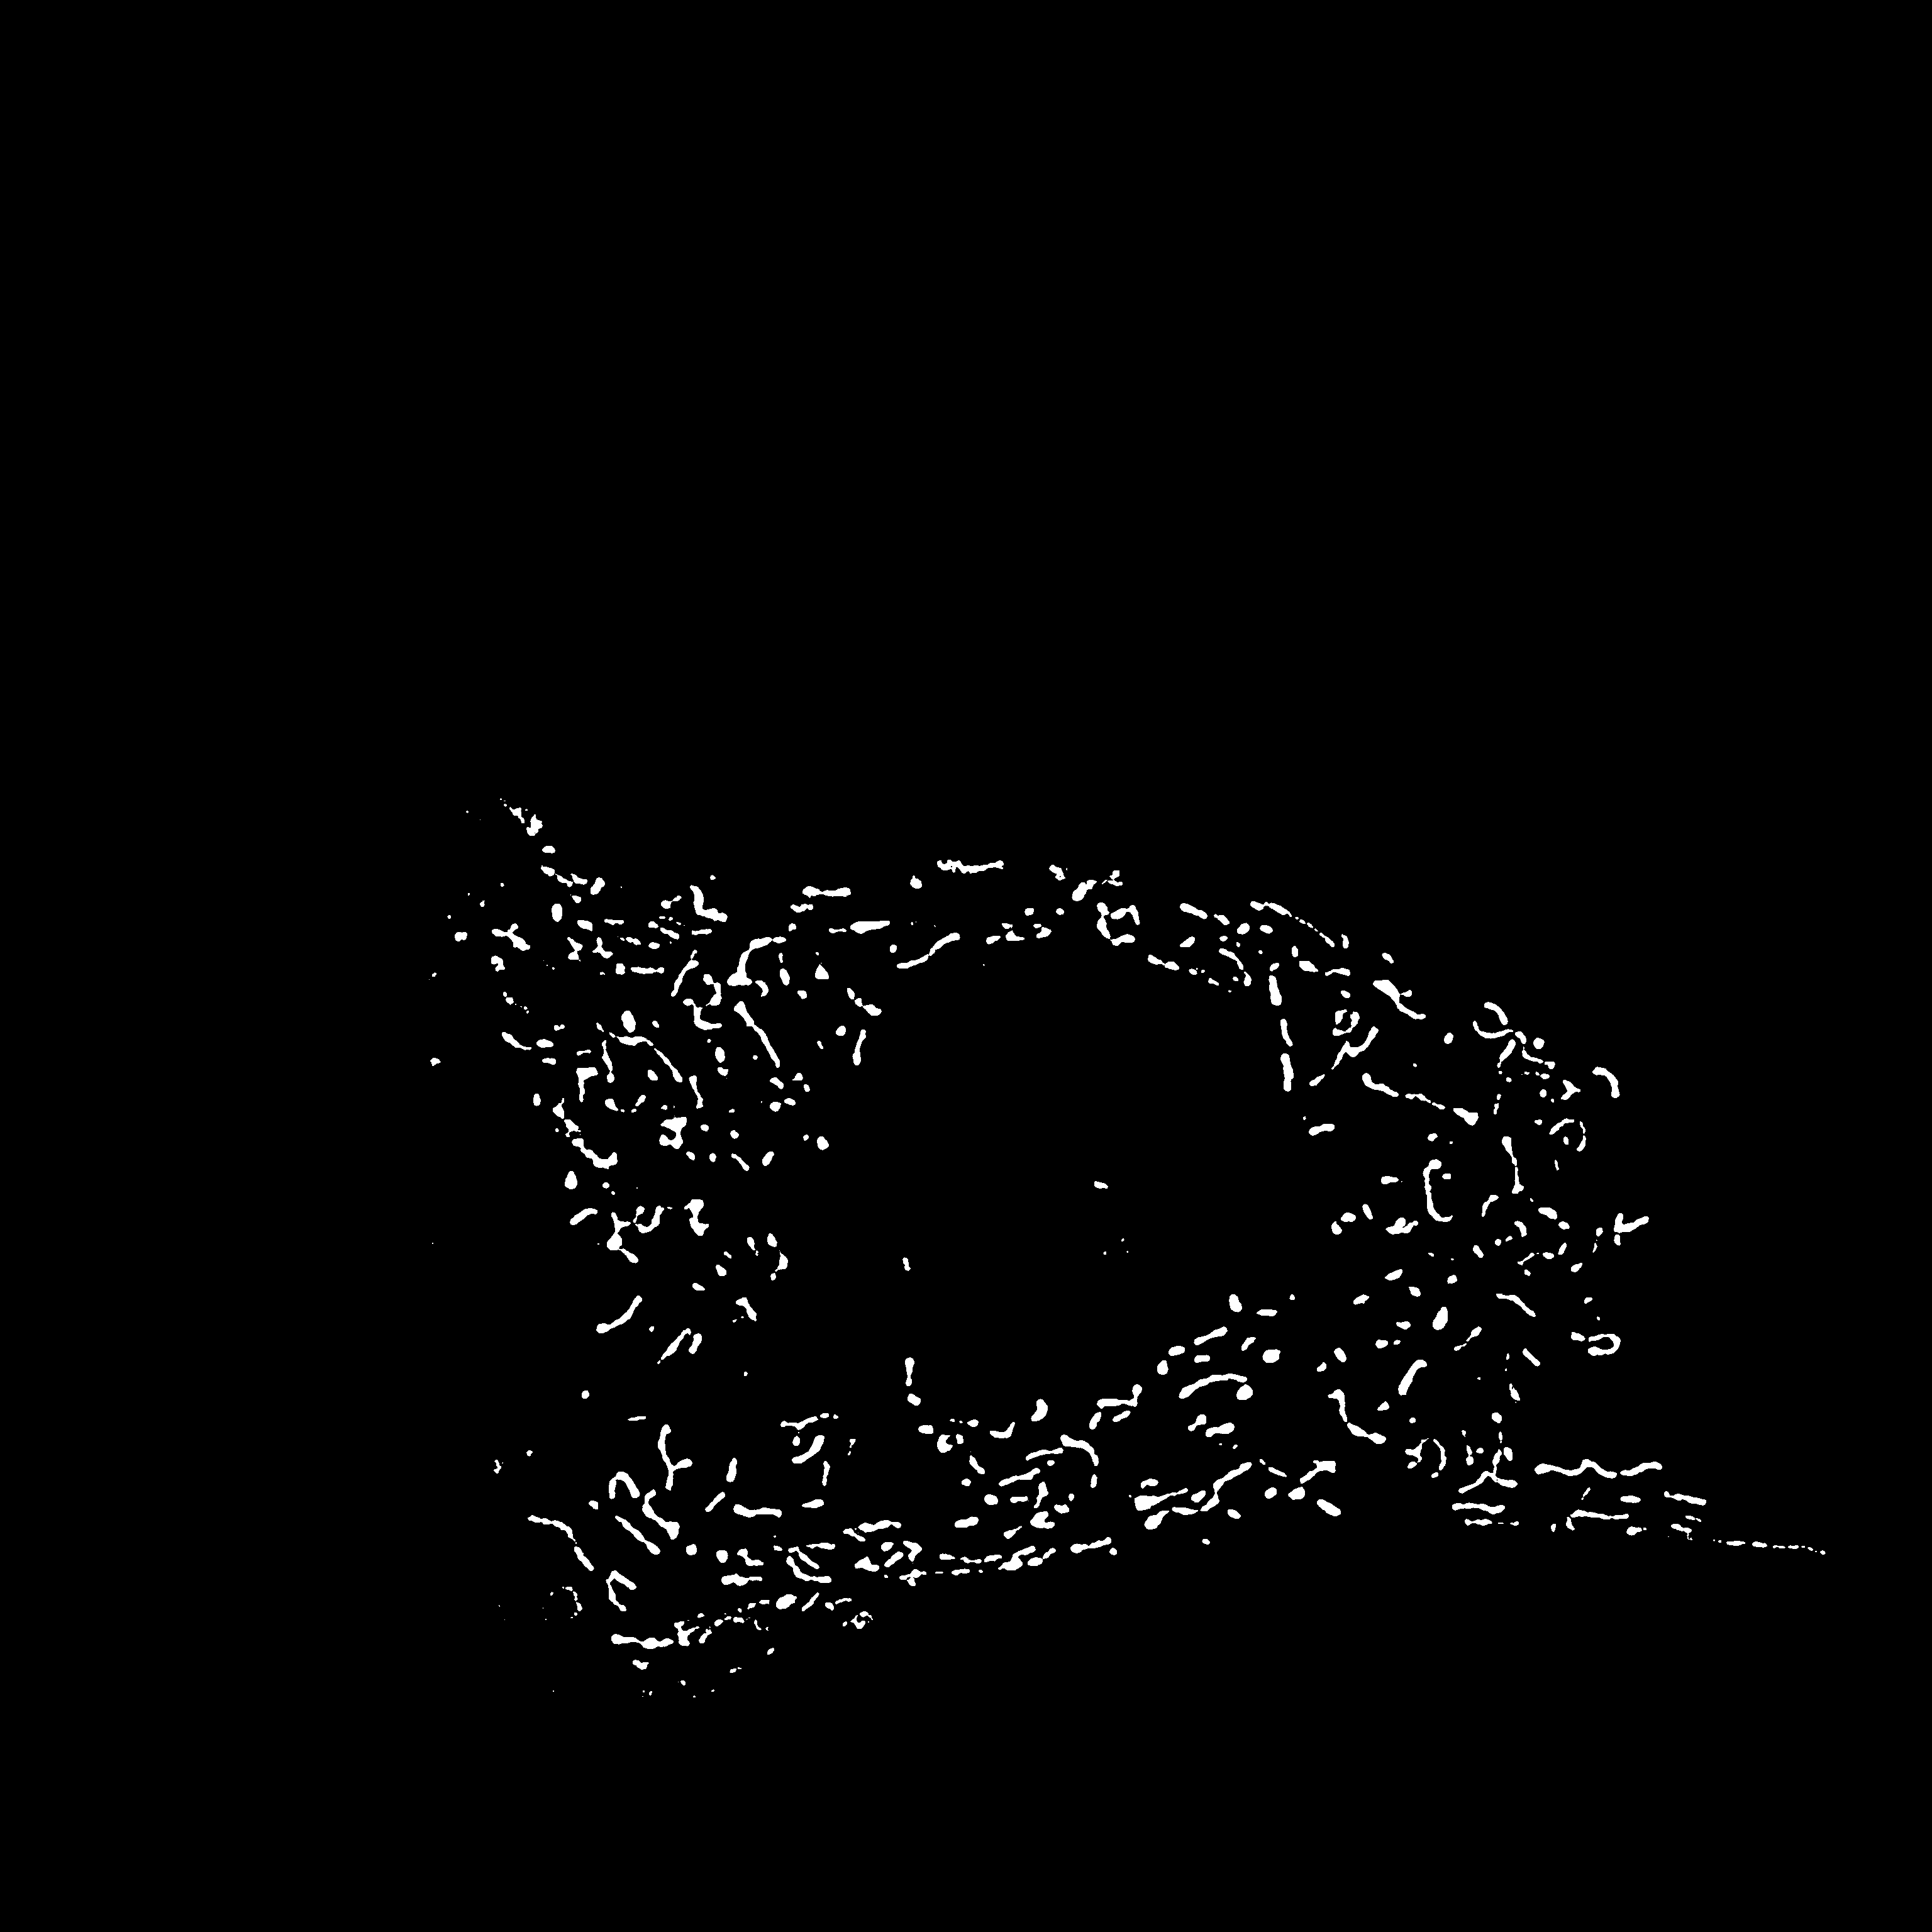
\includegraphics[width=0.2\textwidth]{figs/appendix/method_shortlisting/global_testing/MaxEntropy_CCCP_1C=1T=0.png}}
	\subcaptionbox{Sample 2}{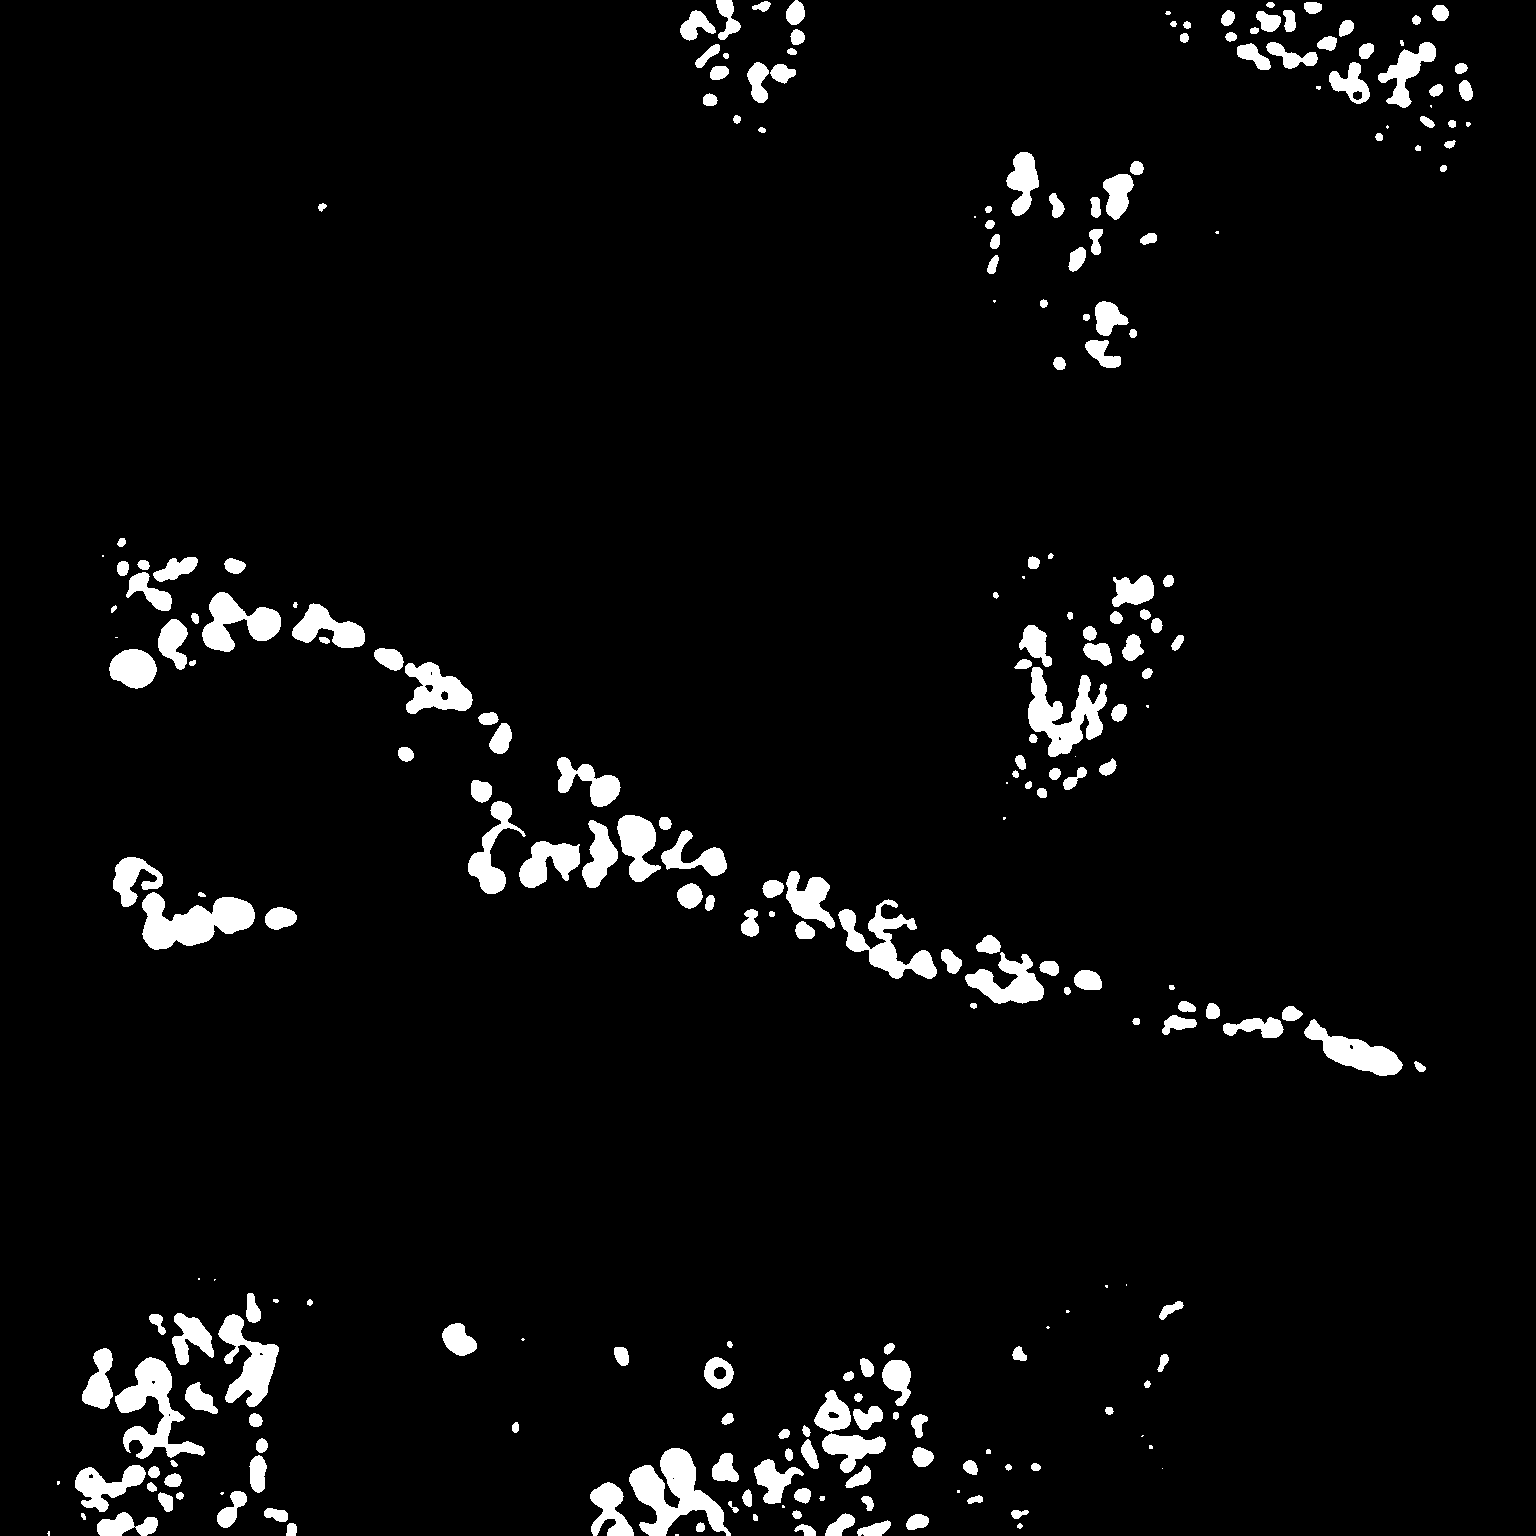
\includegraphics[width=0.2\textwidth]{figs/appendix/method_shortlisting/global_testing/MaxEntropy_HML_4C=0.png}}
	\subcaptionbox{Sample 3}{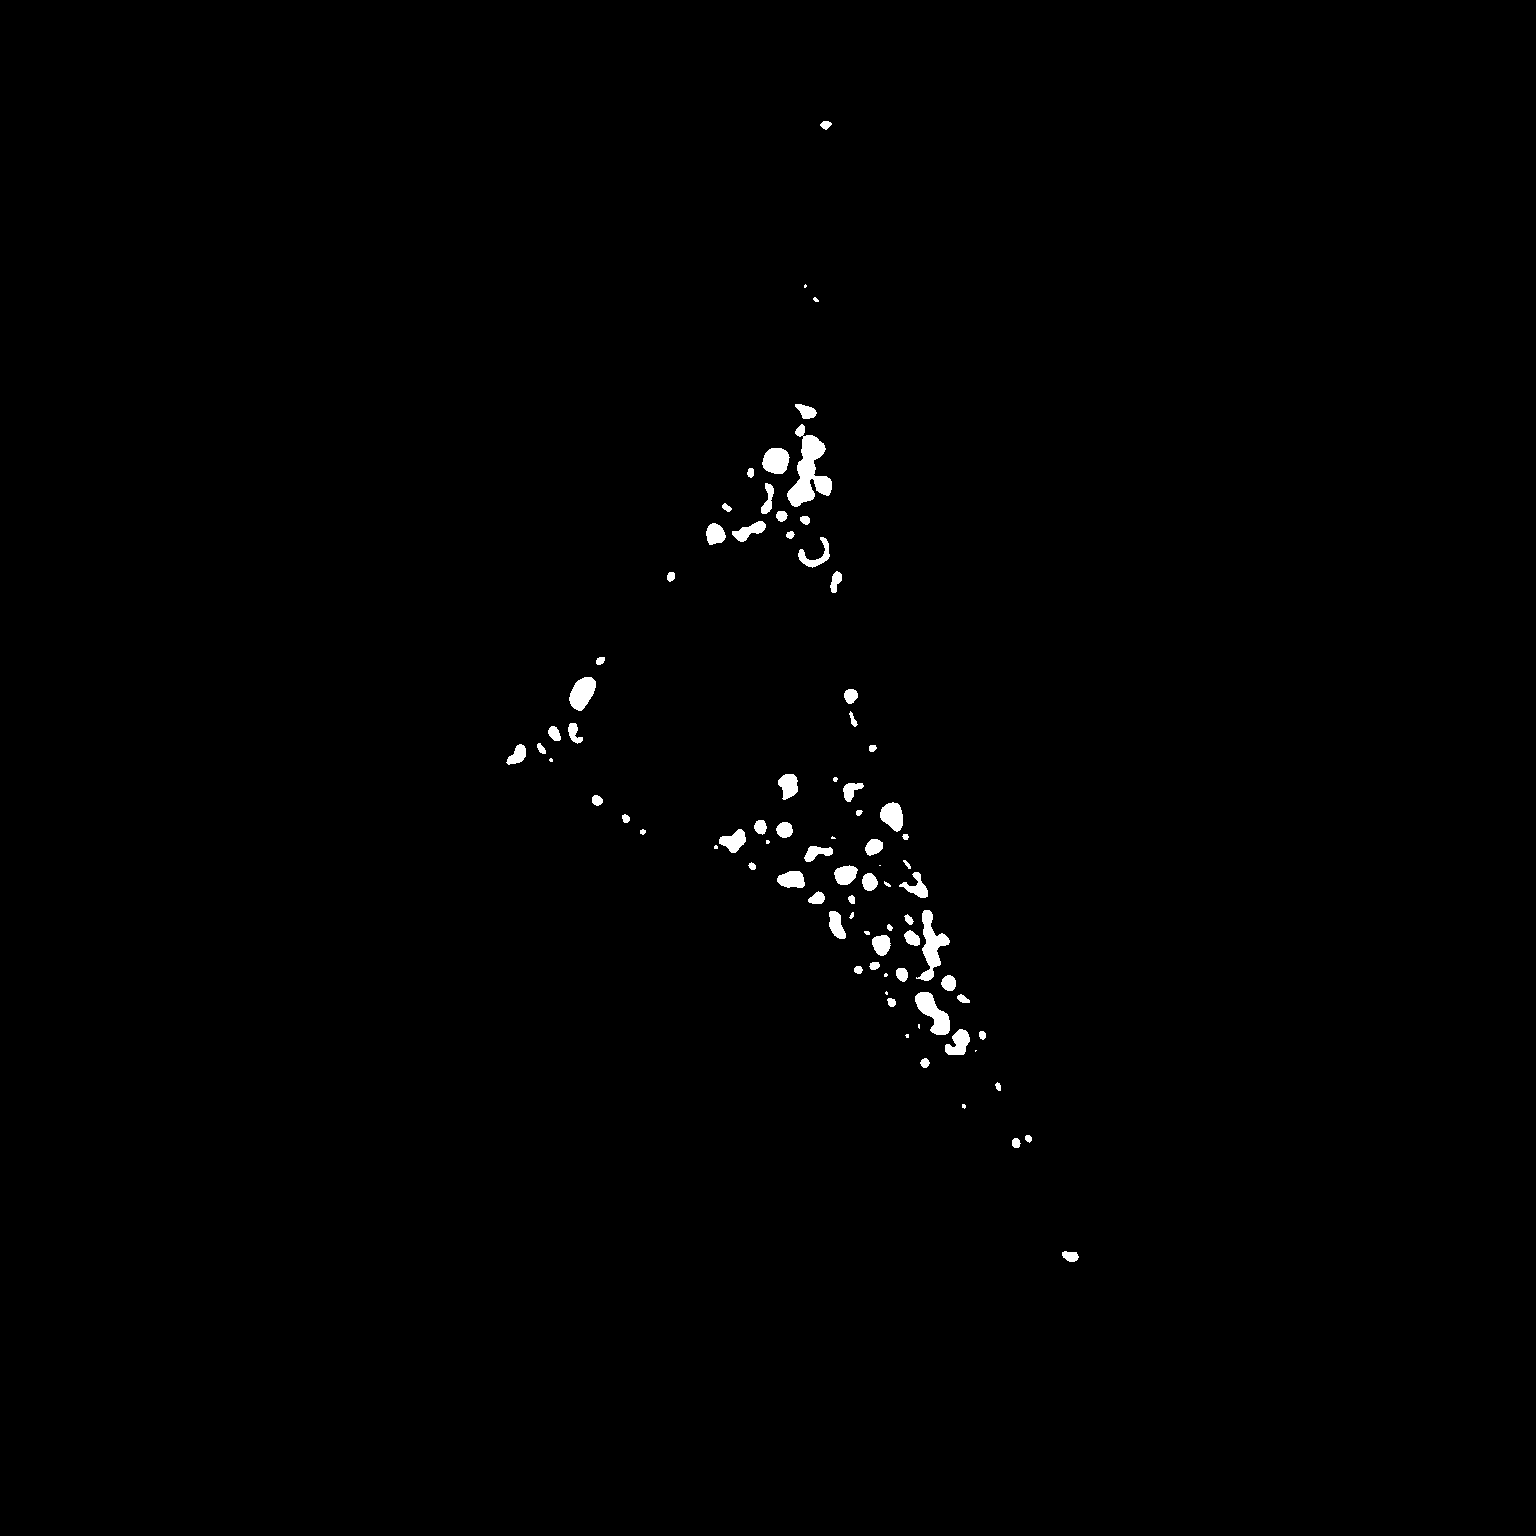
\includegraphics[width=0.2\textwidth]{figs/appendix/method_shortlisting/global_testing/MaxEntropy_LML_3C=0.png}}
	\subcaptionbox{Sample 4}{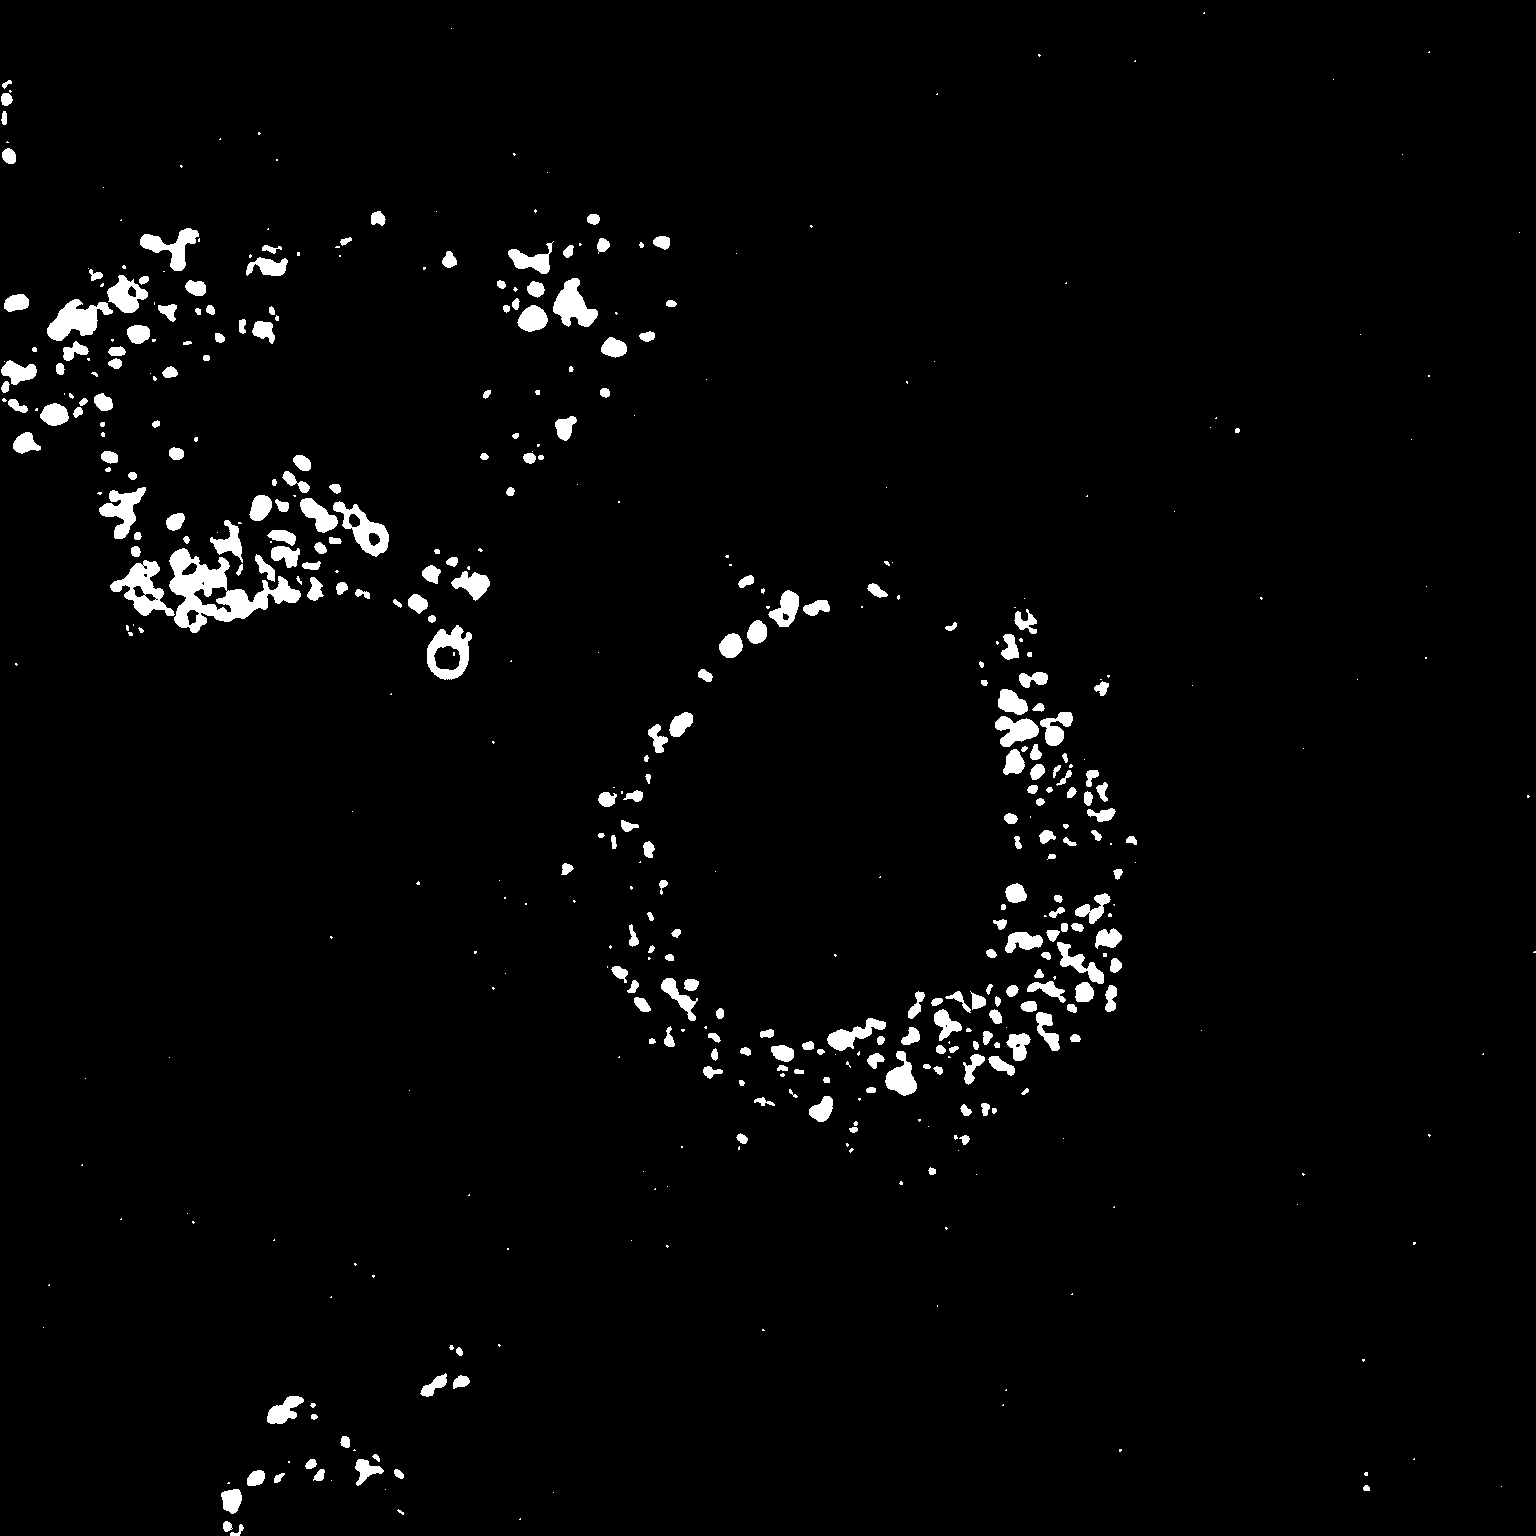
\includegraphics[width=0.2\textwidth]{figs/appendix/method_shortlisting/global_testing/MaxEntropy_LML_4C=1.png}}
	\label{append-fig:MaxEntropy_short}
	\caption{MaxEntropy threshold outcomes for the shortlist sample images}
\end{figure}

\begin{figure}[ht!]
	\centering
	\subcaptionbox{Sample 1}{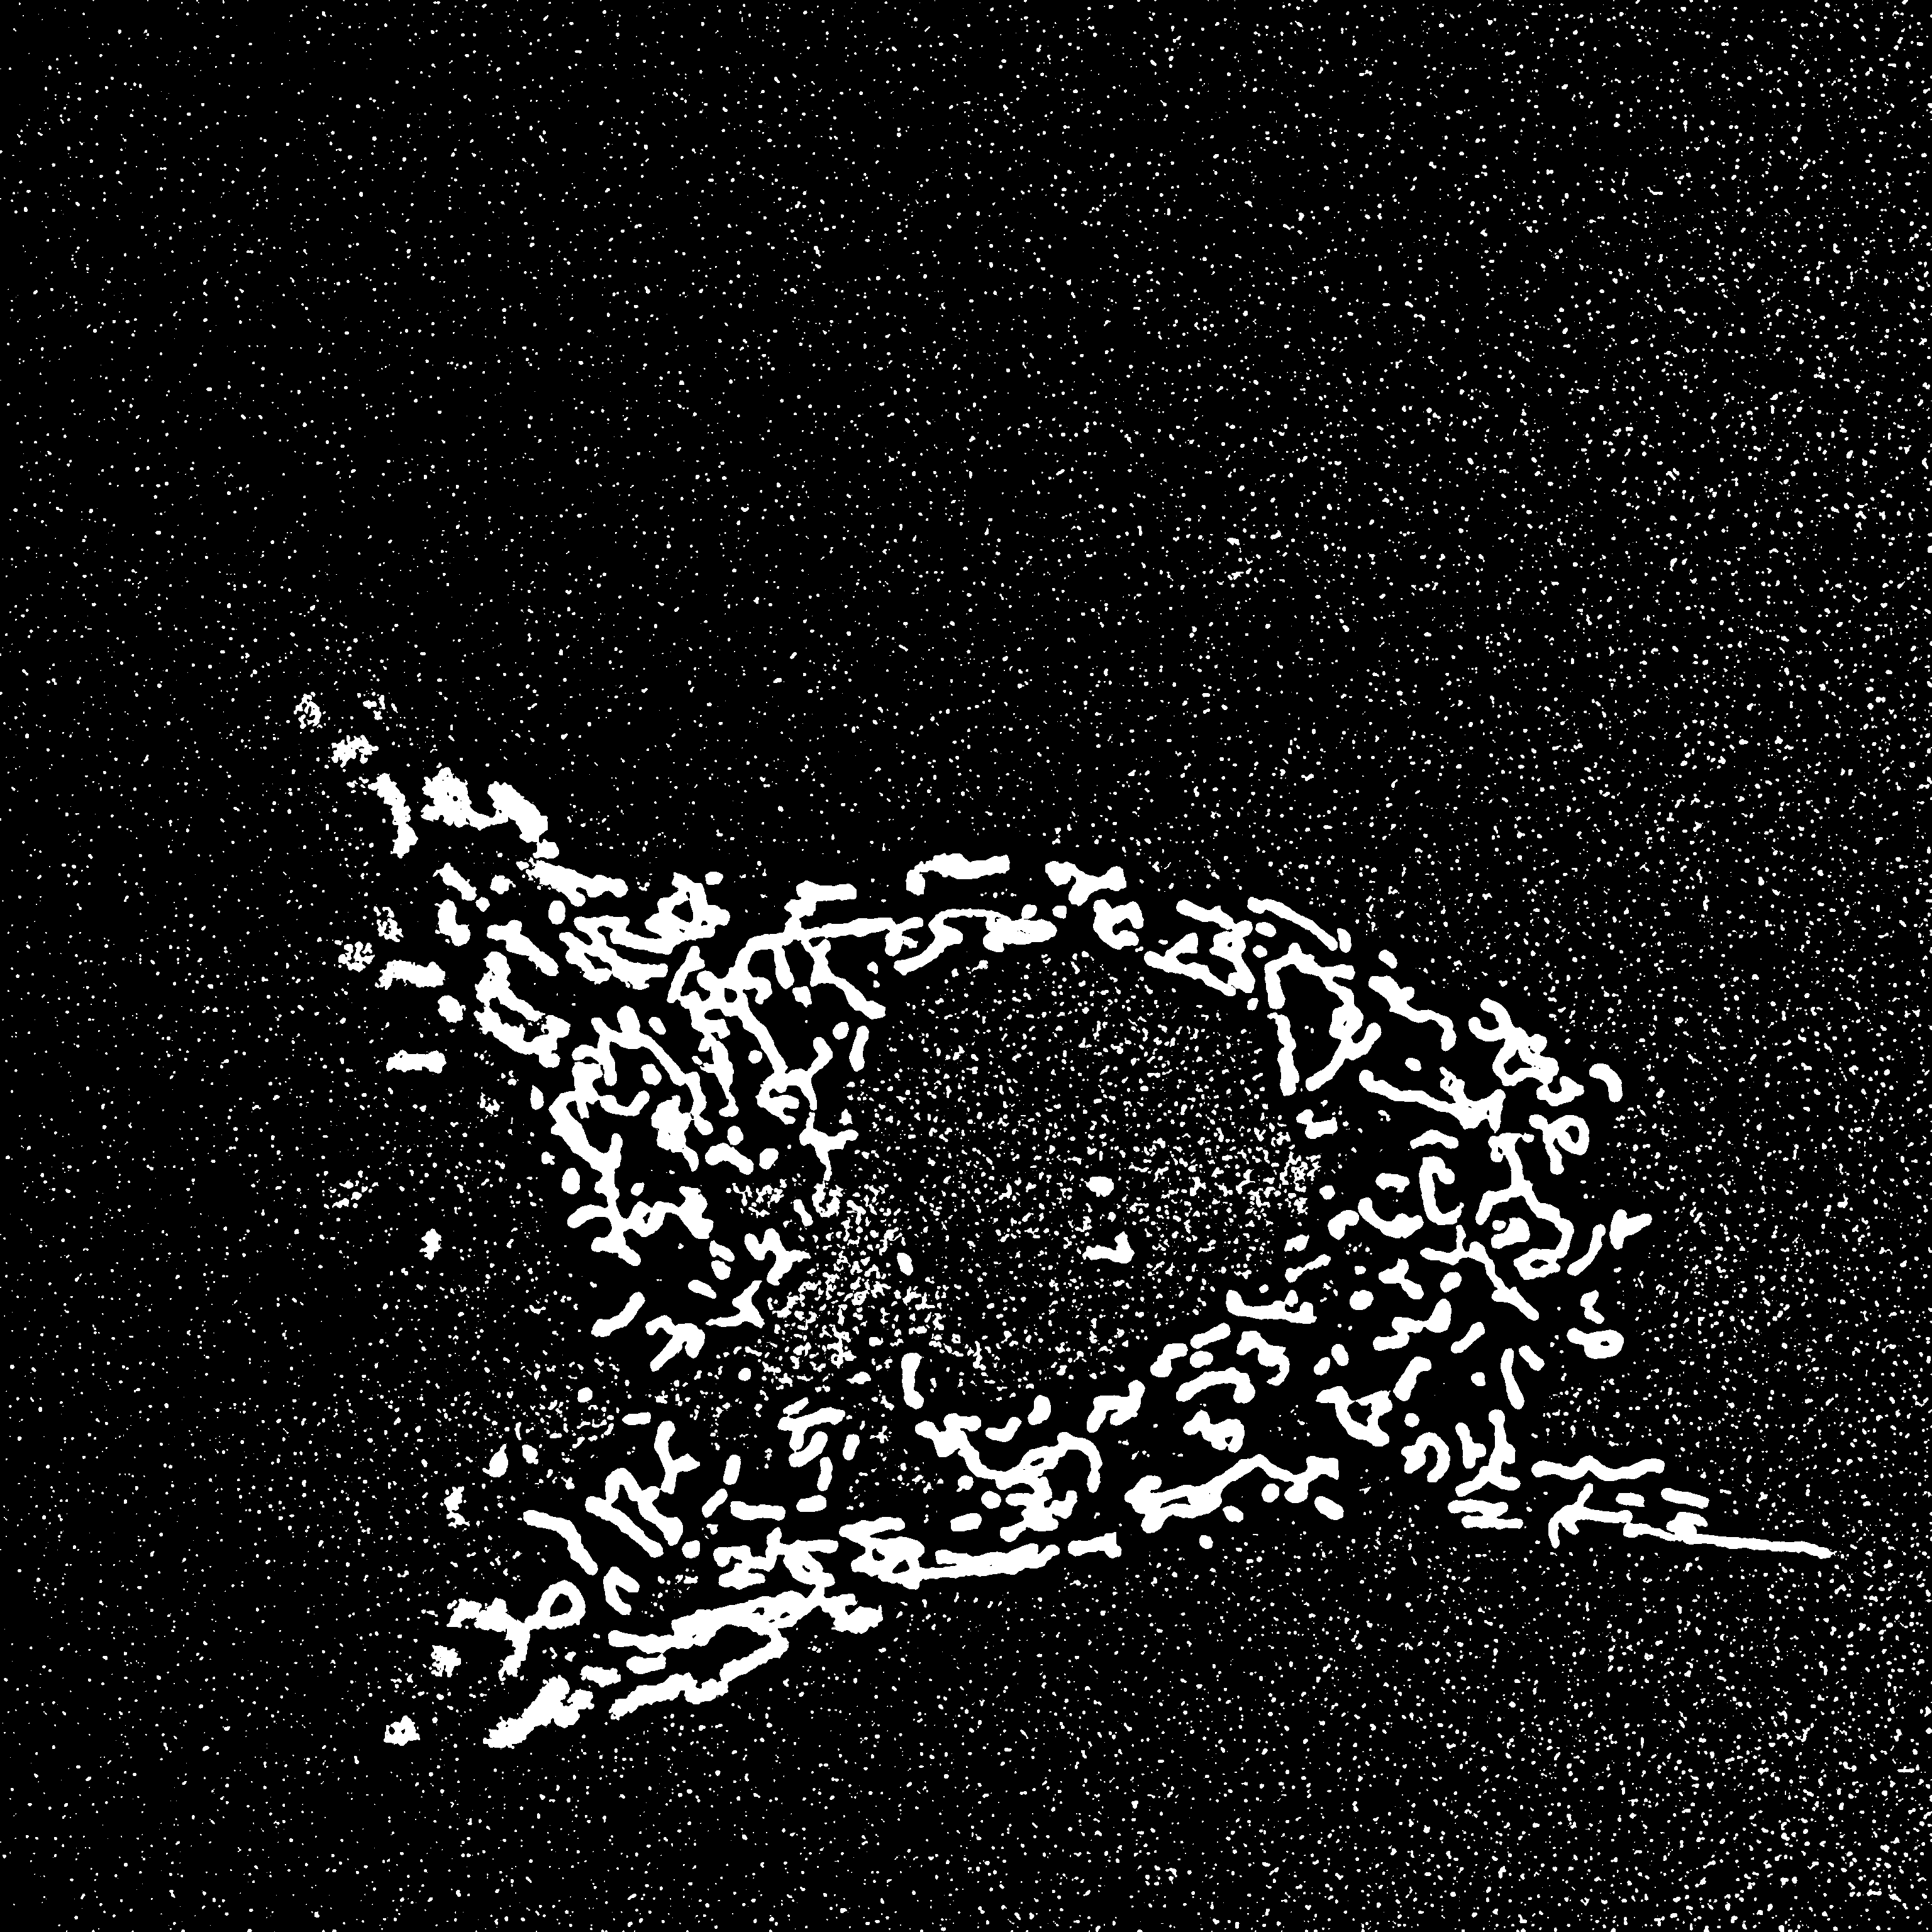
\includegraphics[width=0.2\textwidth]{figs/appendix/method_shortlisting/global_testing/Mean_CCCP_1C=1T=0.png}}
	\subcaptionbox{Sample 2}{
\includegraphics[width=0.2\textwidth]{figs/appendix/method_shortlisting/global_testing/Mean_HML_4C=0.png}}
	\subcaptionbox{Sample 3}{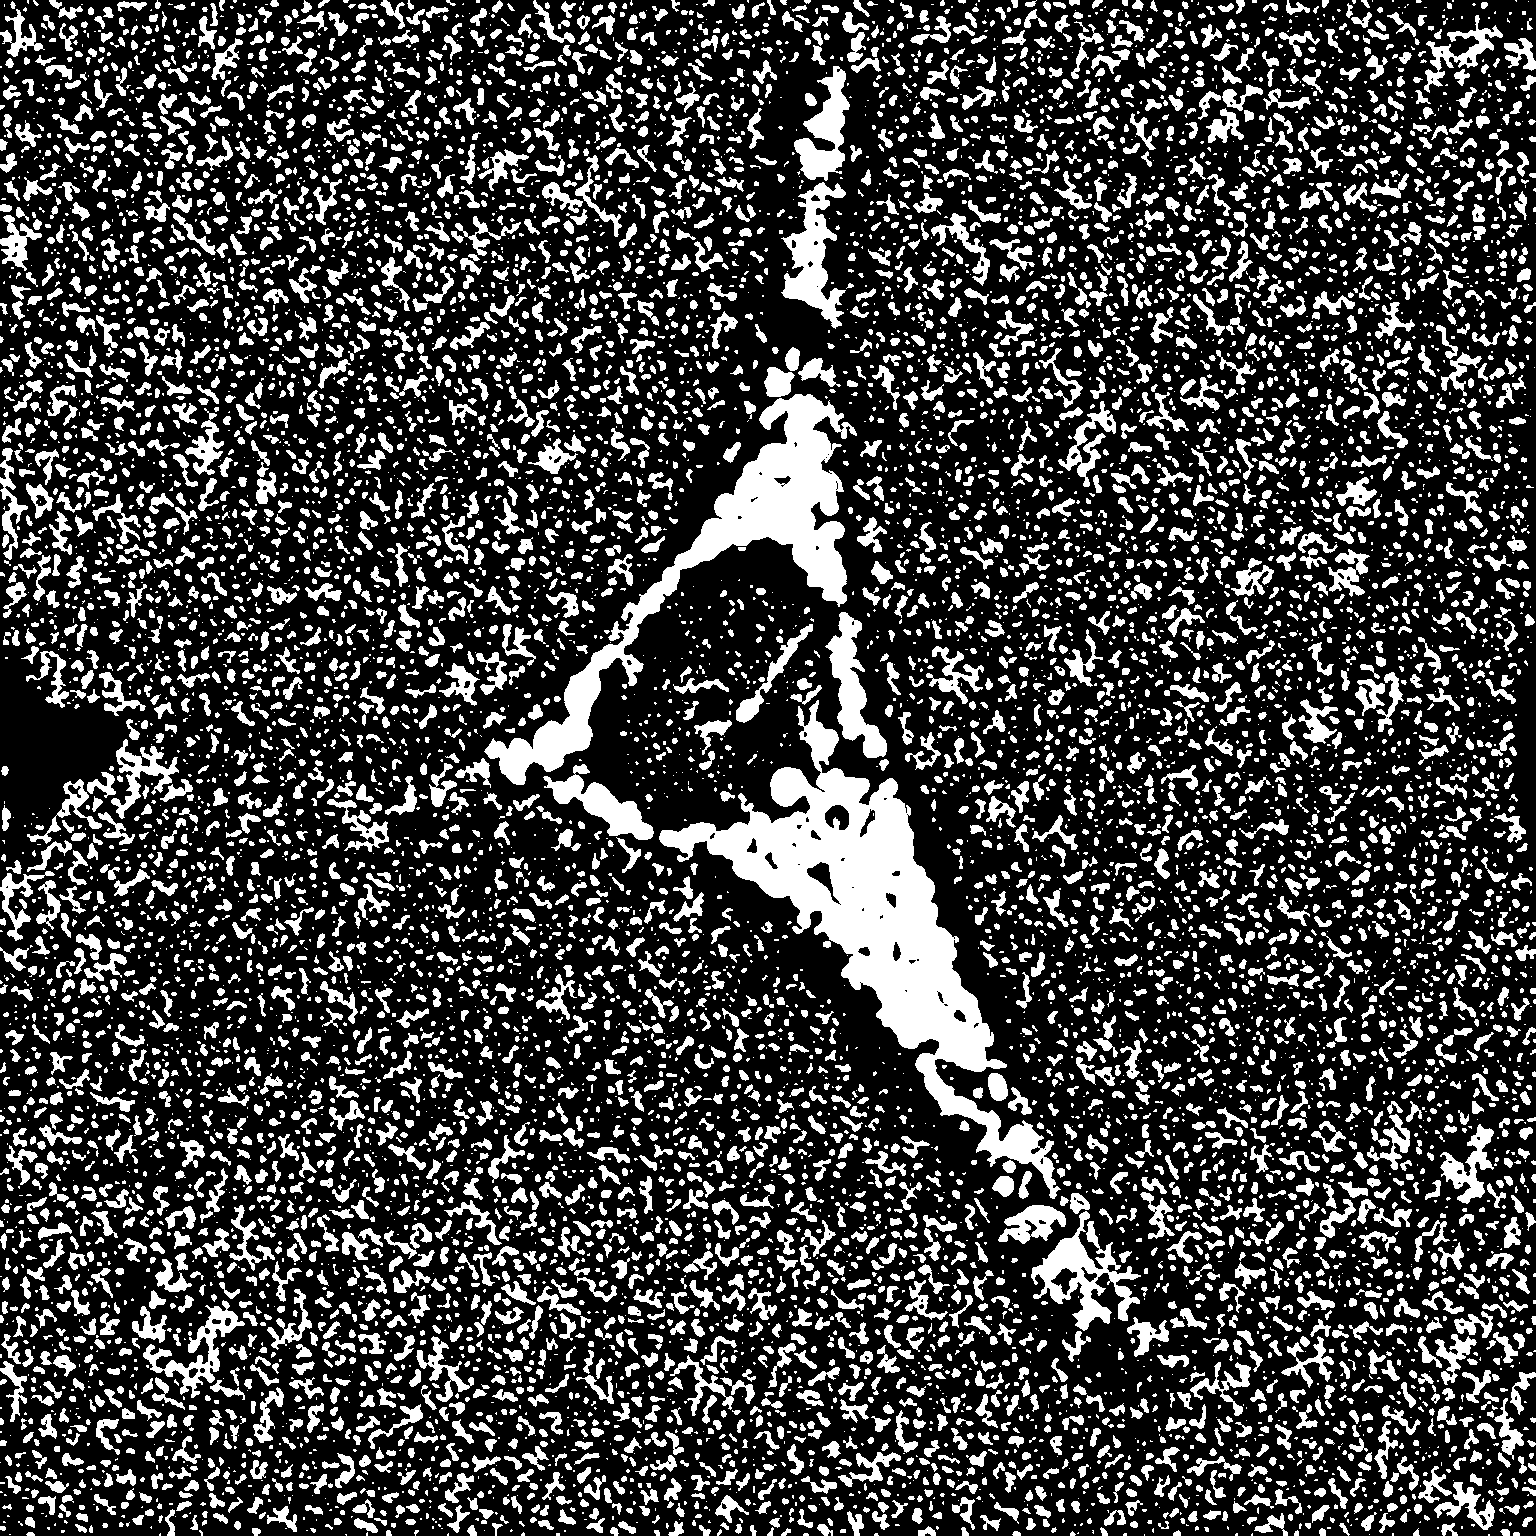
\includegraphics[width=0.2\textwidth]{figs/appendix/method_shortlisting/global_testing/Mean_LML_3C=0.png}}
	\subcaptionbox{Sample 4}{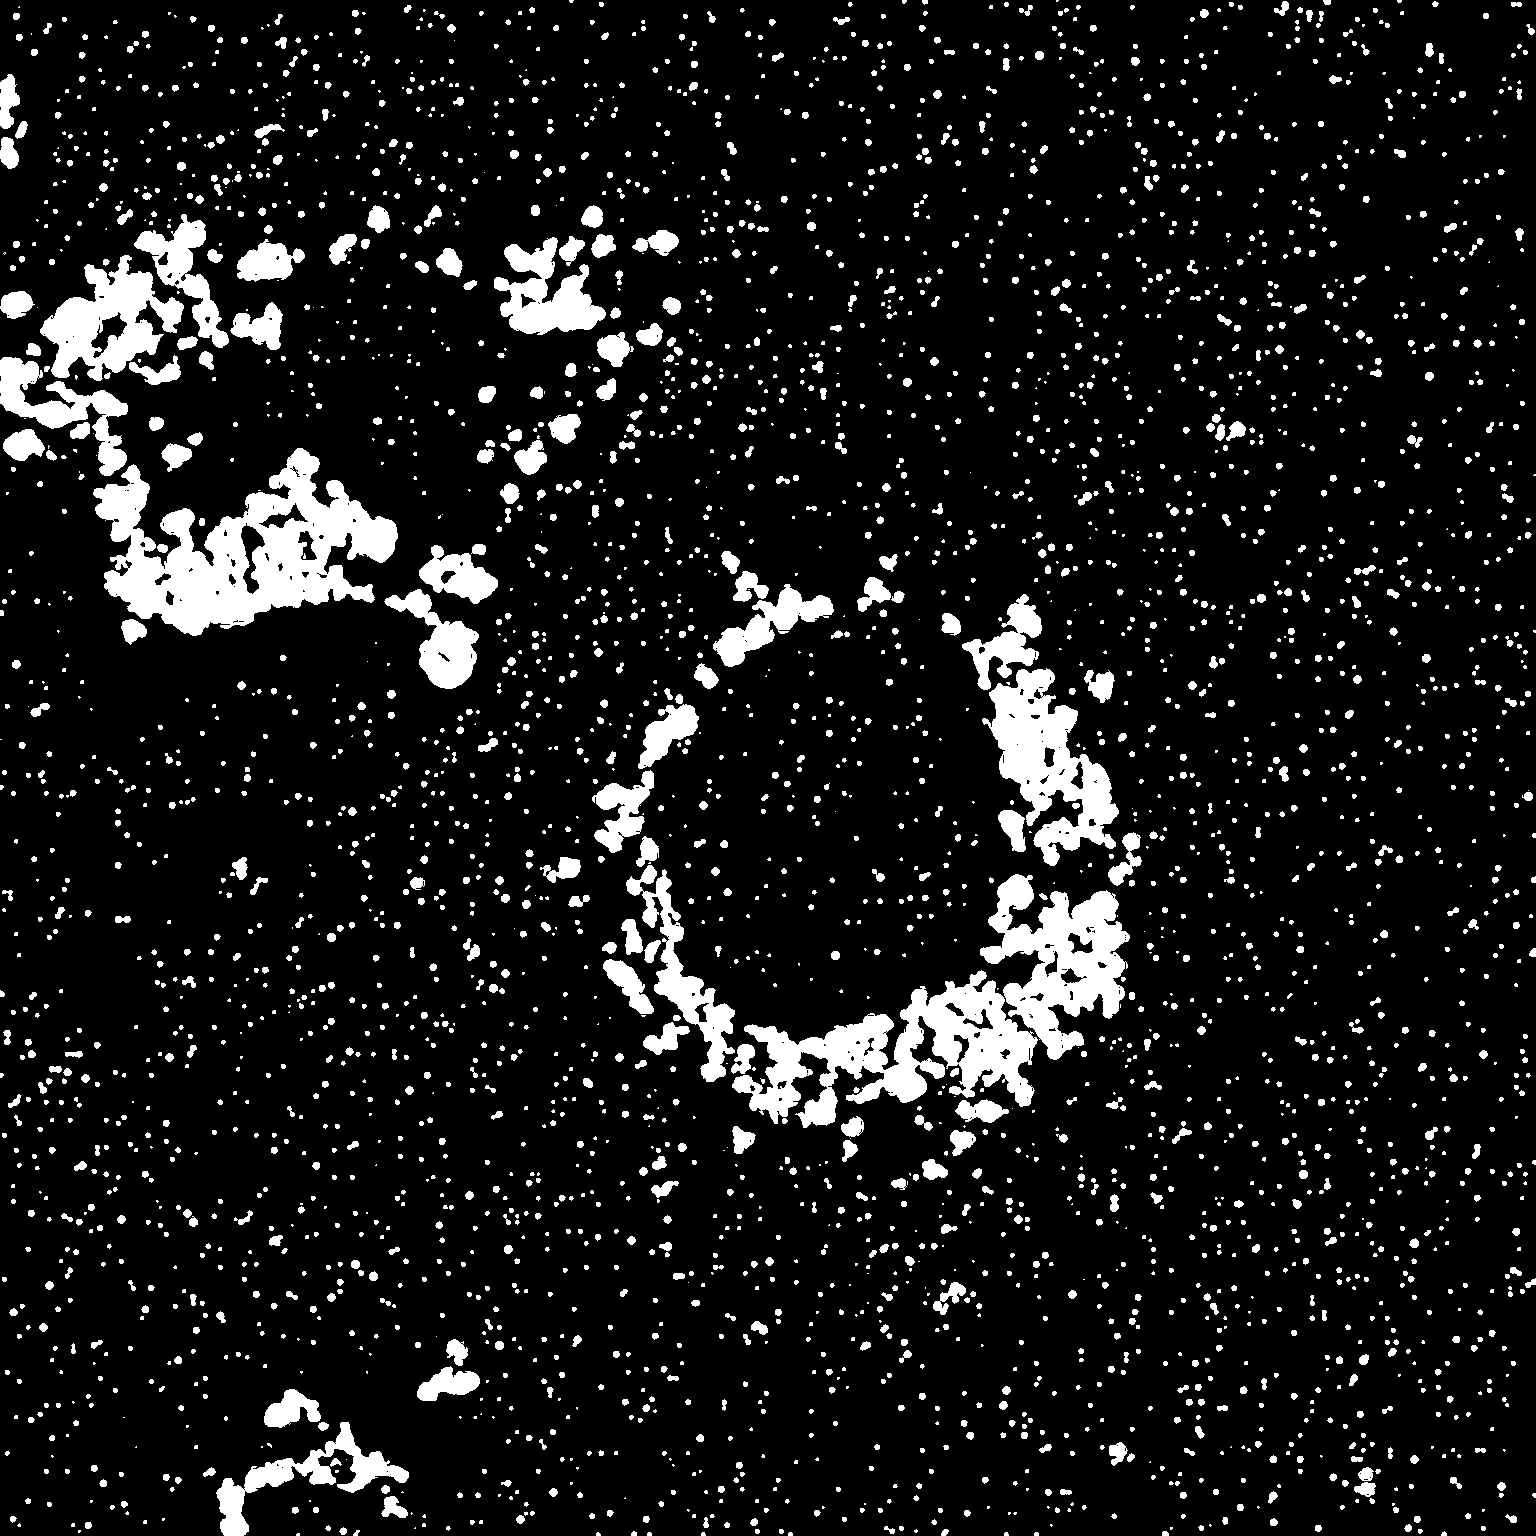
\includegraphics[width=0.2\textwidth]{figs/appendix/method_shortlisting/global_testing/Mean_LML_4C=1.png}}
	\label{append-fig:Mean_short}
	\caption{Mean threshold outcomes for the shortlist sample images}
\end{figure}

\begin{figure}[ht!]
	\centering
	\subcaptionbox{Sample 1}{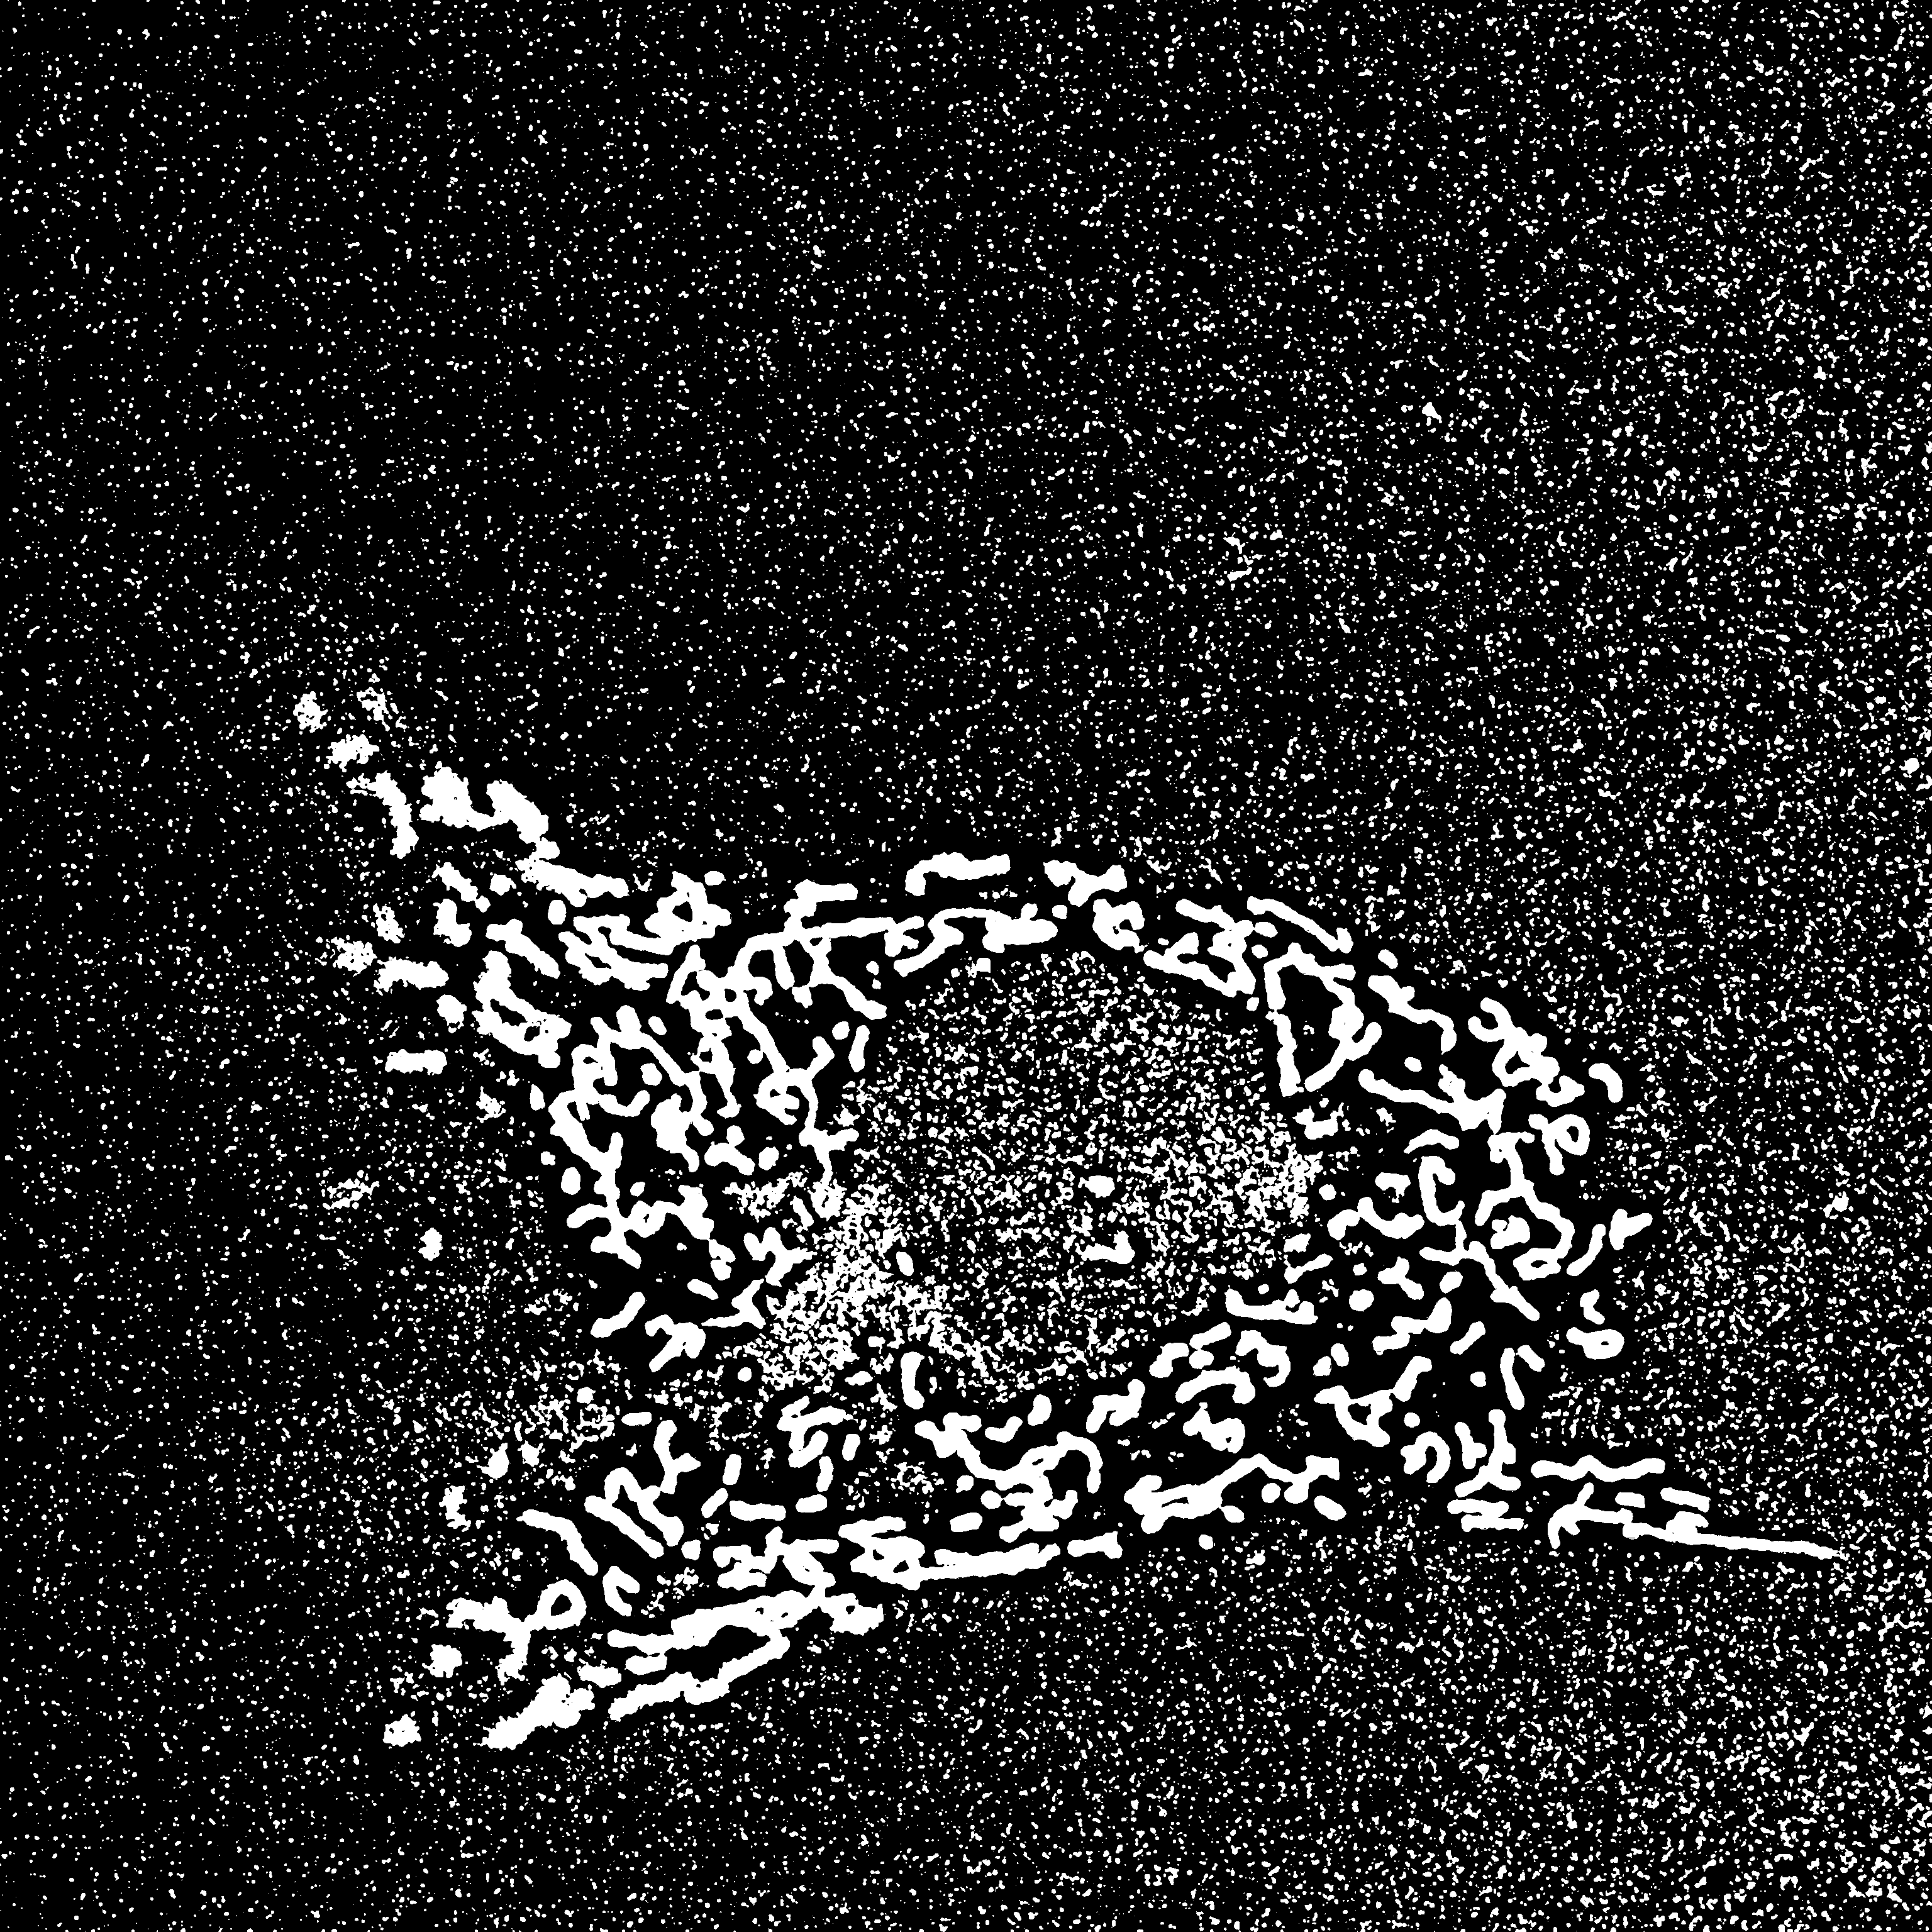
\includegraphics[width=0.2\textwidth]{figs/appendix/method_shortlisting/global_testing/MinError(I)_CCCP_1C=1T=0.png}}
	\subcaptionbox{Sample 2}{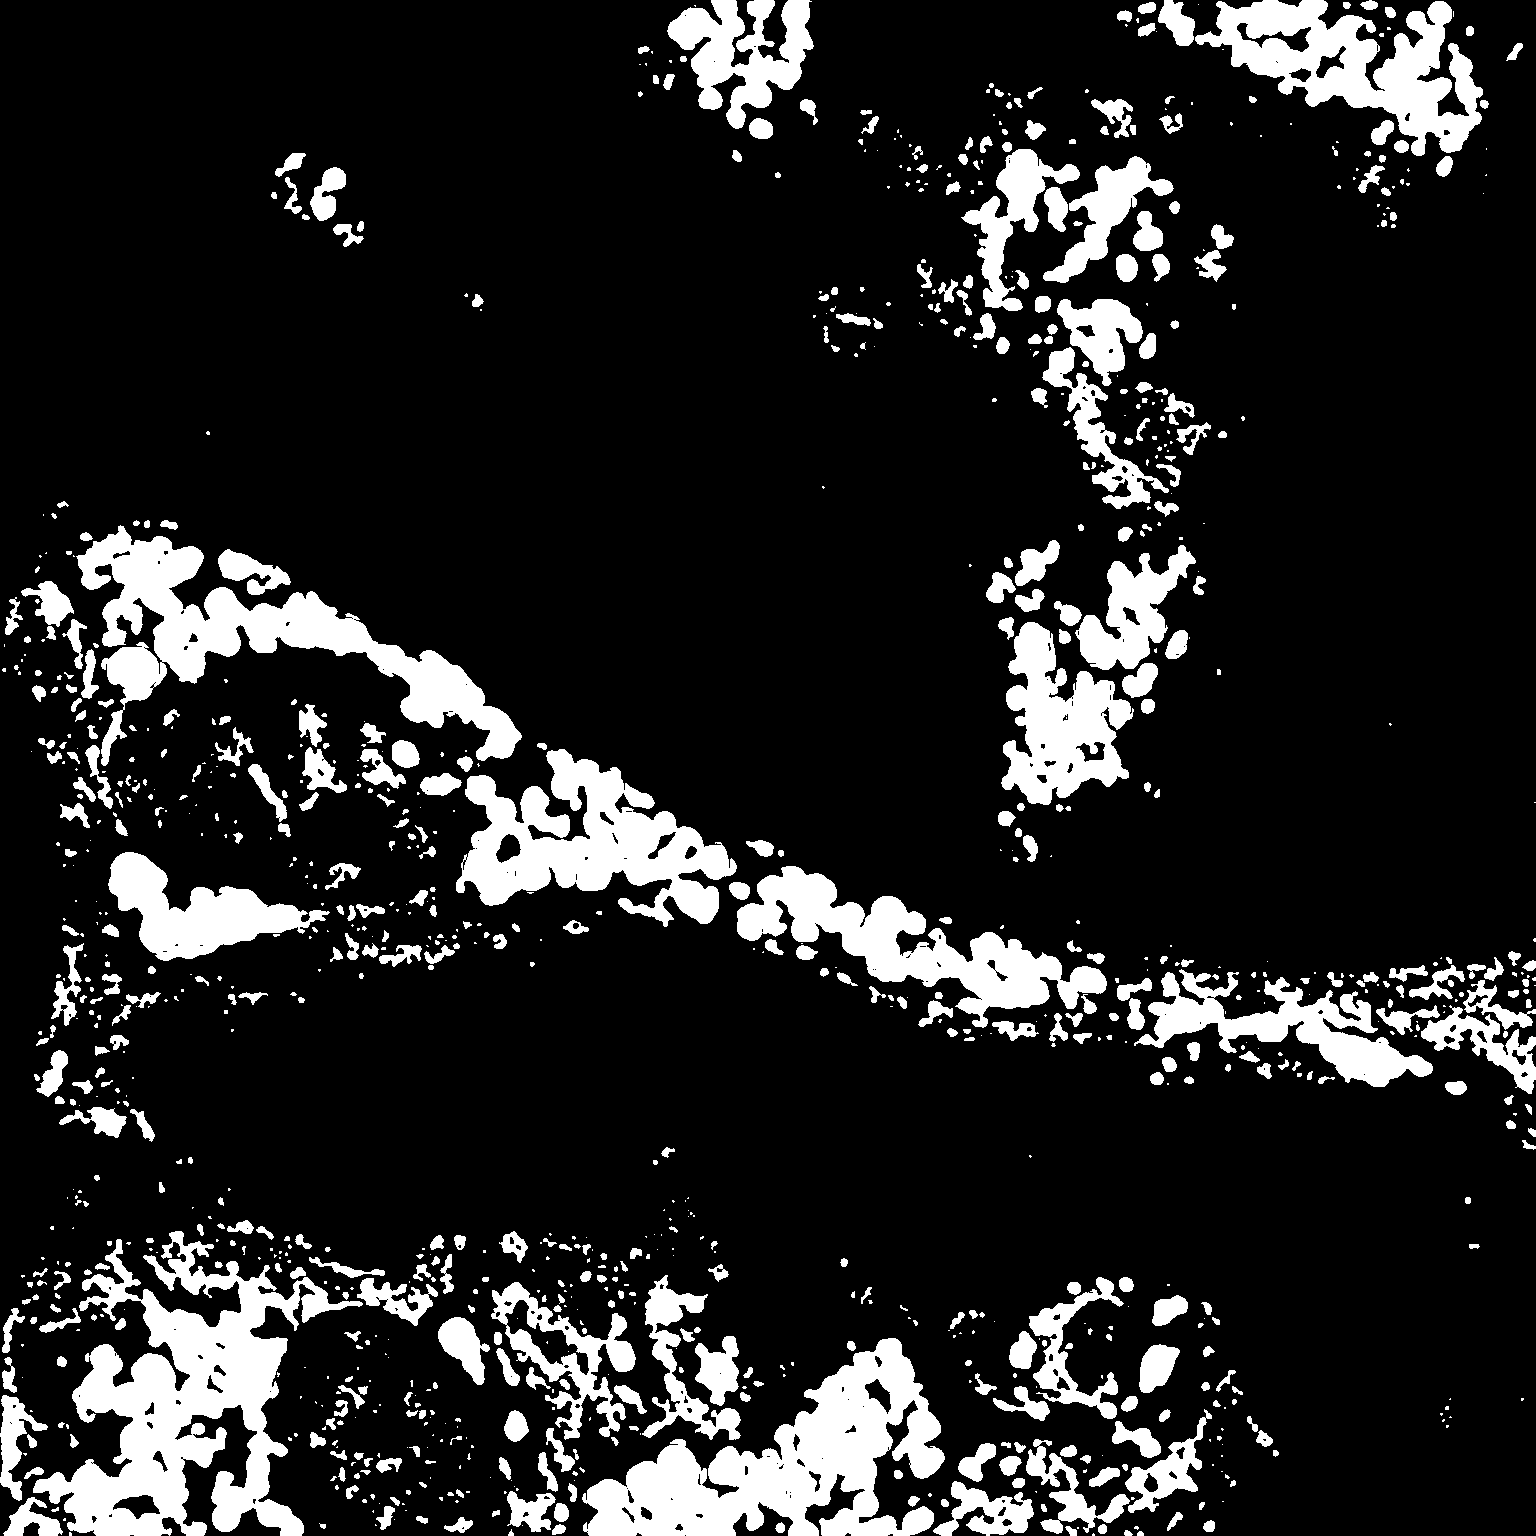
\includegraphics[width=0.2\textwidth]{figs/appendix/method_shortlisting/global_testing/MinError(I)_HML_4C=0.png}}
	\subcaptionbox{Sample 3}{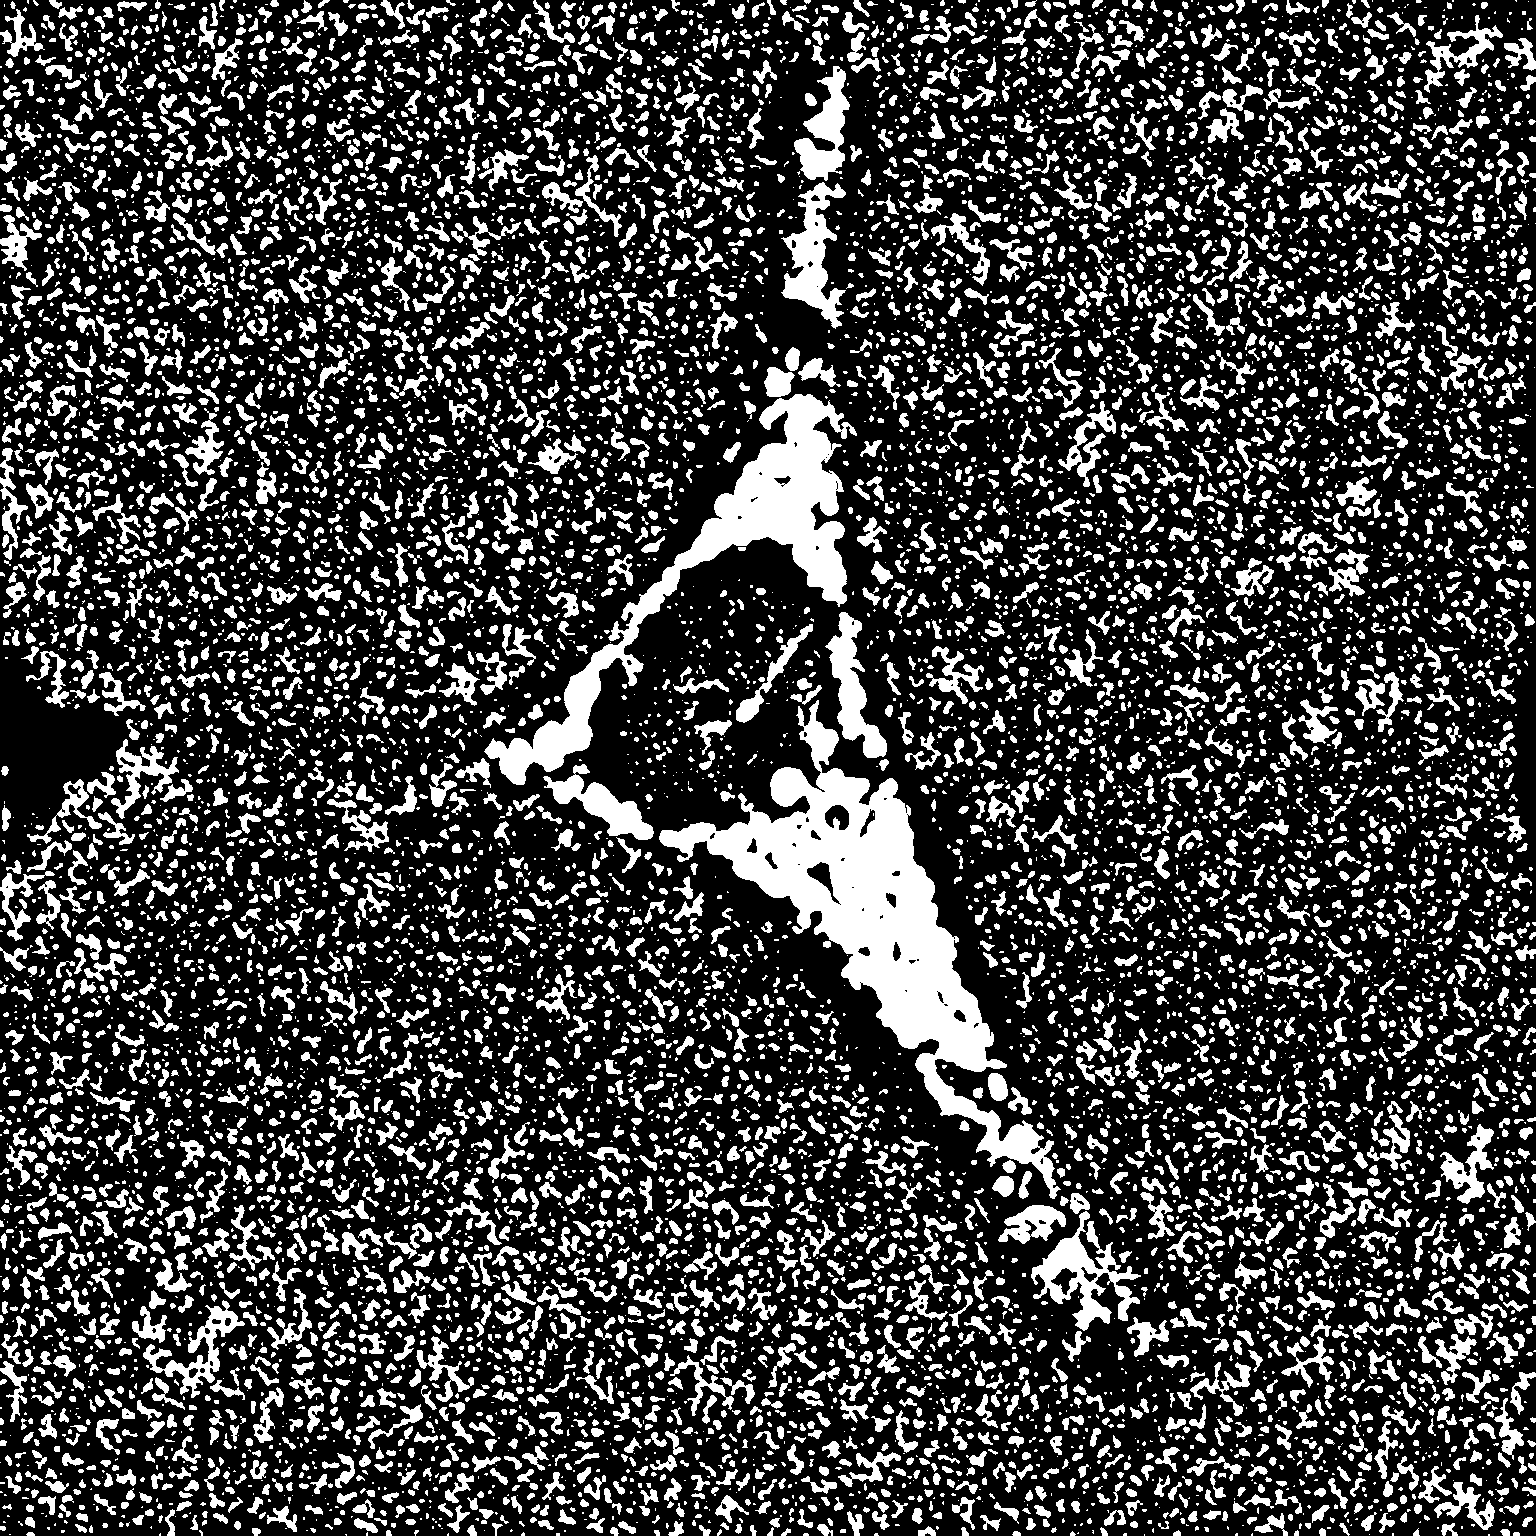
\includegraphics[width=0.2\textwidth]{figs/appendix/method_shortlisting/global_testing/MinError(I)_LML_3C=0.png}}
	\subcaptionbox{Sample 4}{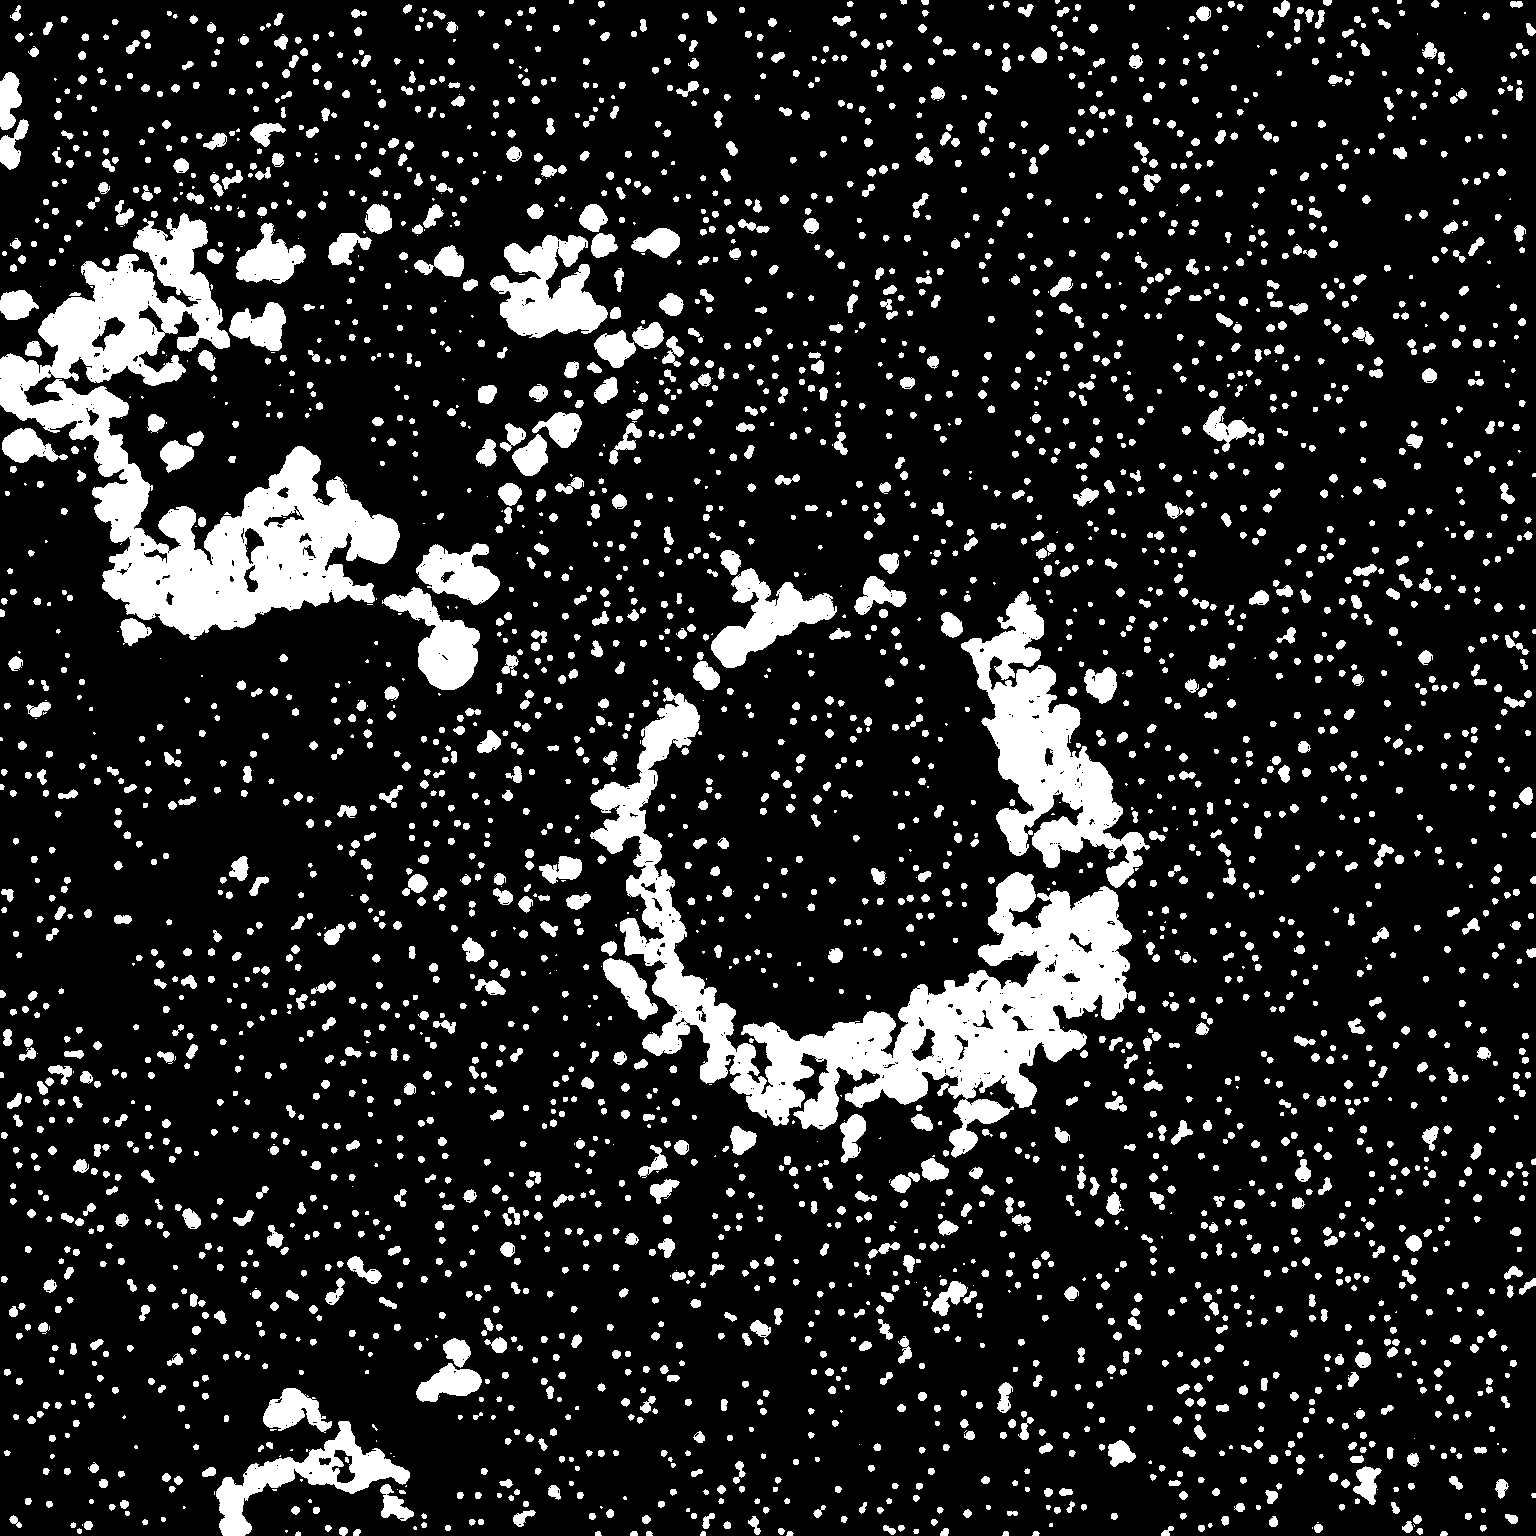
\includegraphics[width=0.2\textwidth]{figs/appendix/method_shortlisting/global_testing/MinError(I)_LML_4C=1.png}}
	\label{append-fig:MinError_short}
	\caption{MinError(I) threshold outcomes for the shortlist sample images}
\end{figure}

\begin{figure}[ht!]
	\centering
	\subcaptionbox{Sample 1}{
\includegraphics[width=0.2\textwidth]{figs/appendix/method_shortlisting/global_testing/Minimum_CCCP_1C=1T=0.png}}
	\subcaptionbox{Sample 2}{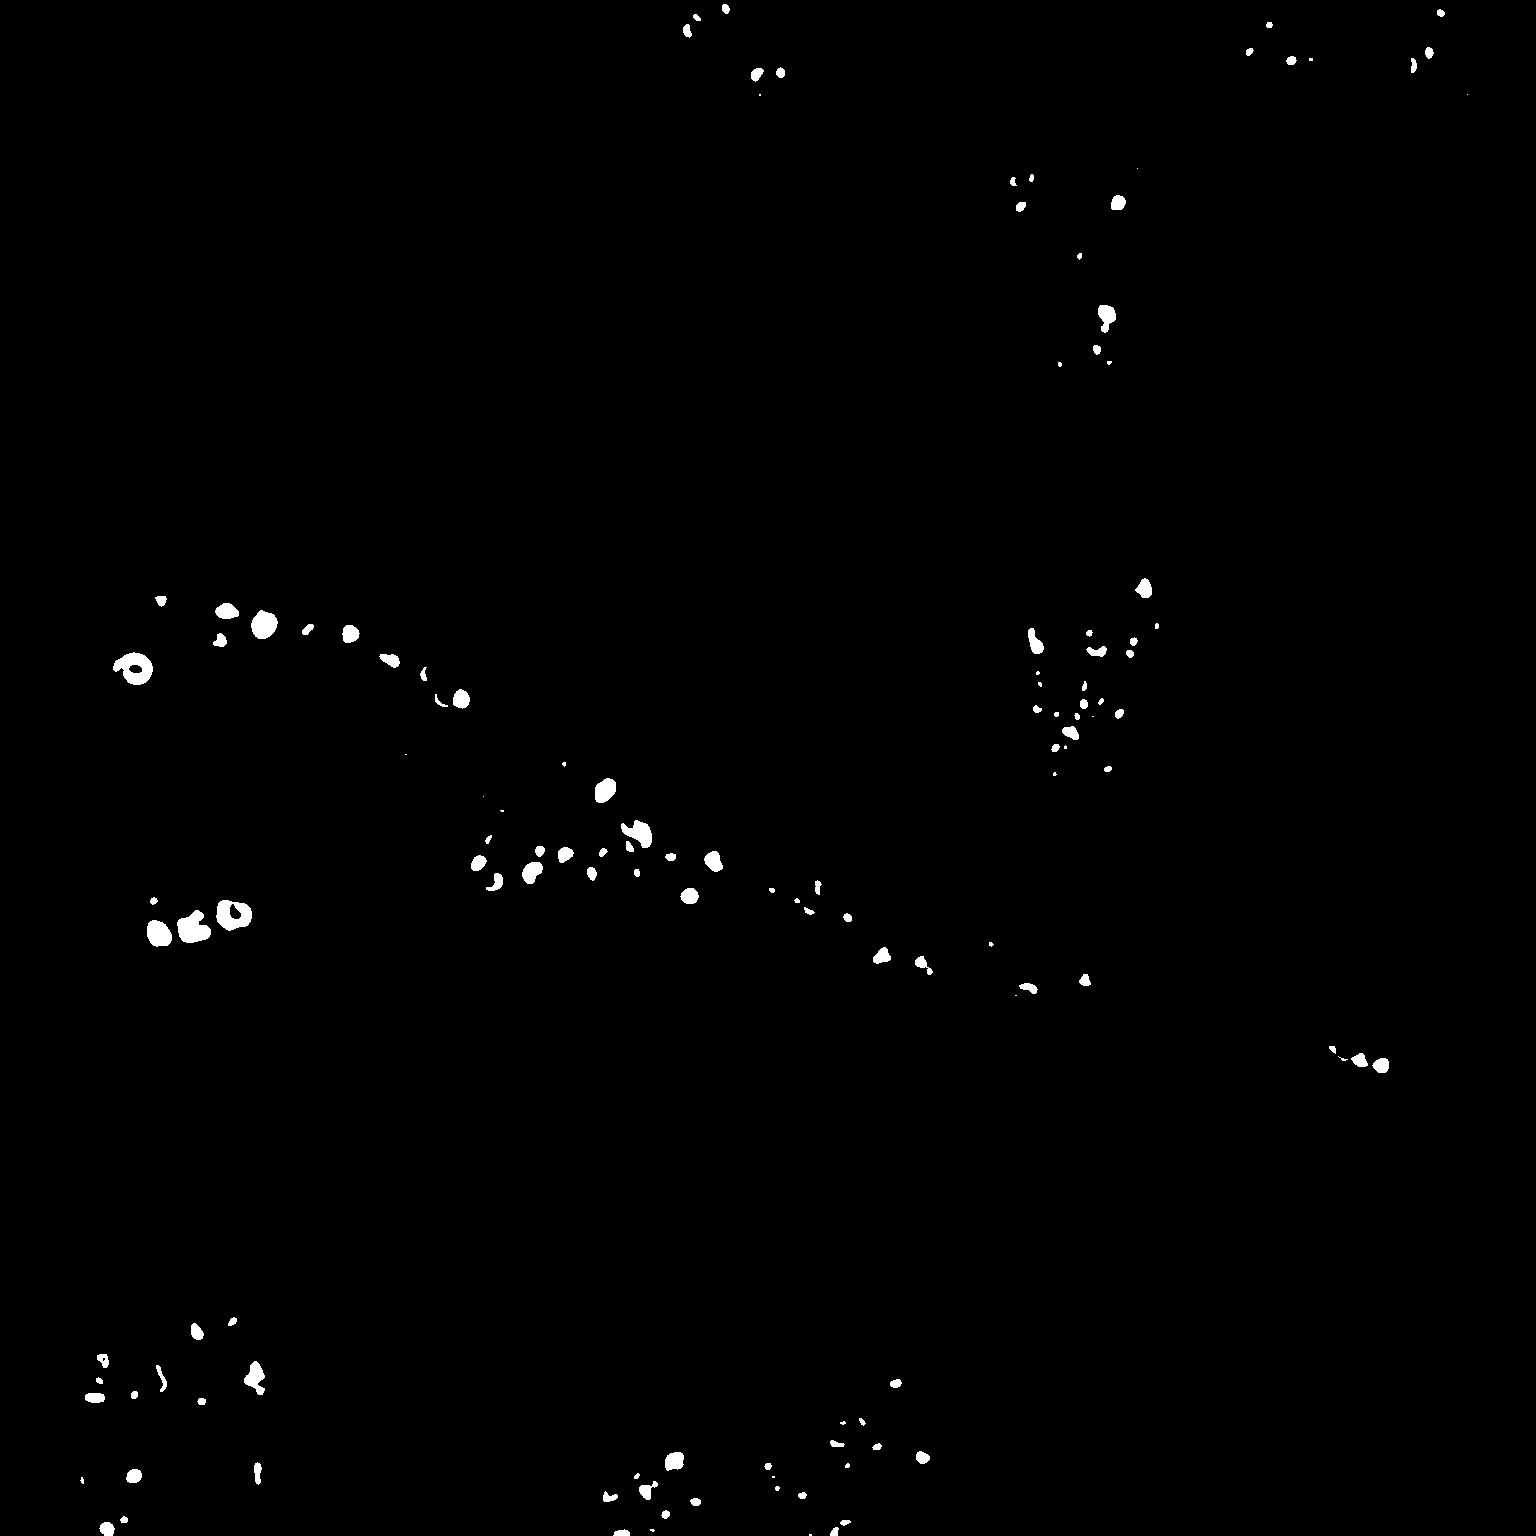
\includegraphics[width=0.2\textwidth]{figs/appendix/method_shortlisting/global_testing/Minimum_HML_4C=0.png}}
	\subcaptionbox{Sample 3}{
\includegraphics[width=0.2\textwidth]{figs/appendix/method_shortlisting/global_testing/Minimum_LML_3C=0.png}}
	\subcaptionbox{Sample 4}{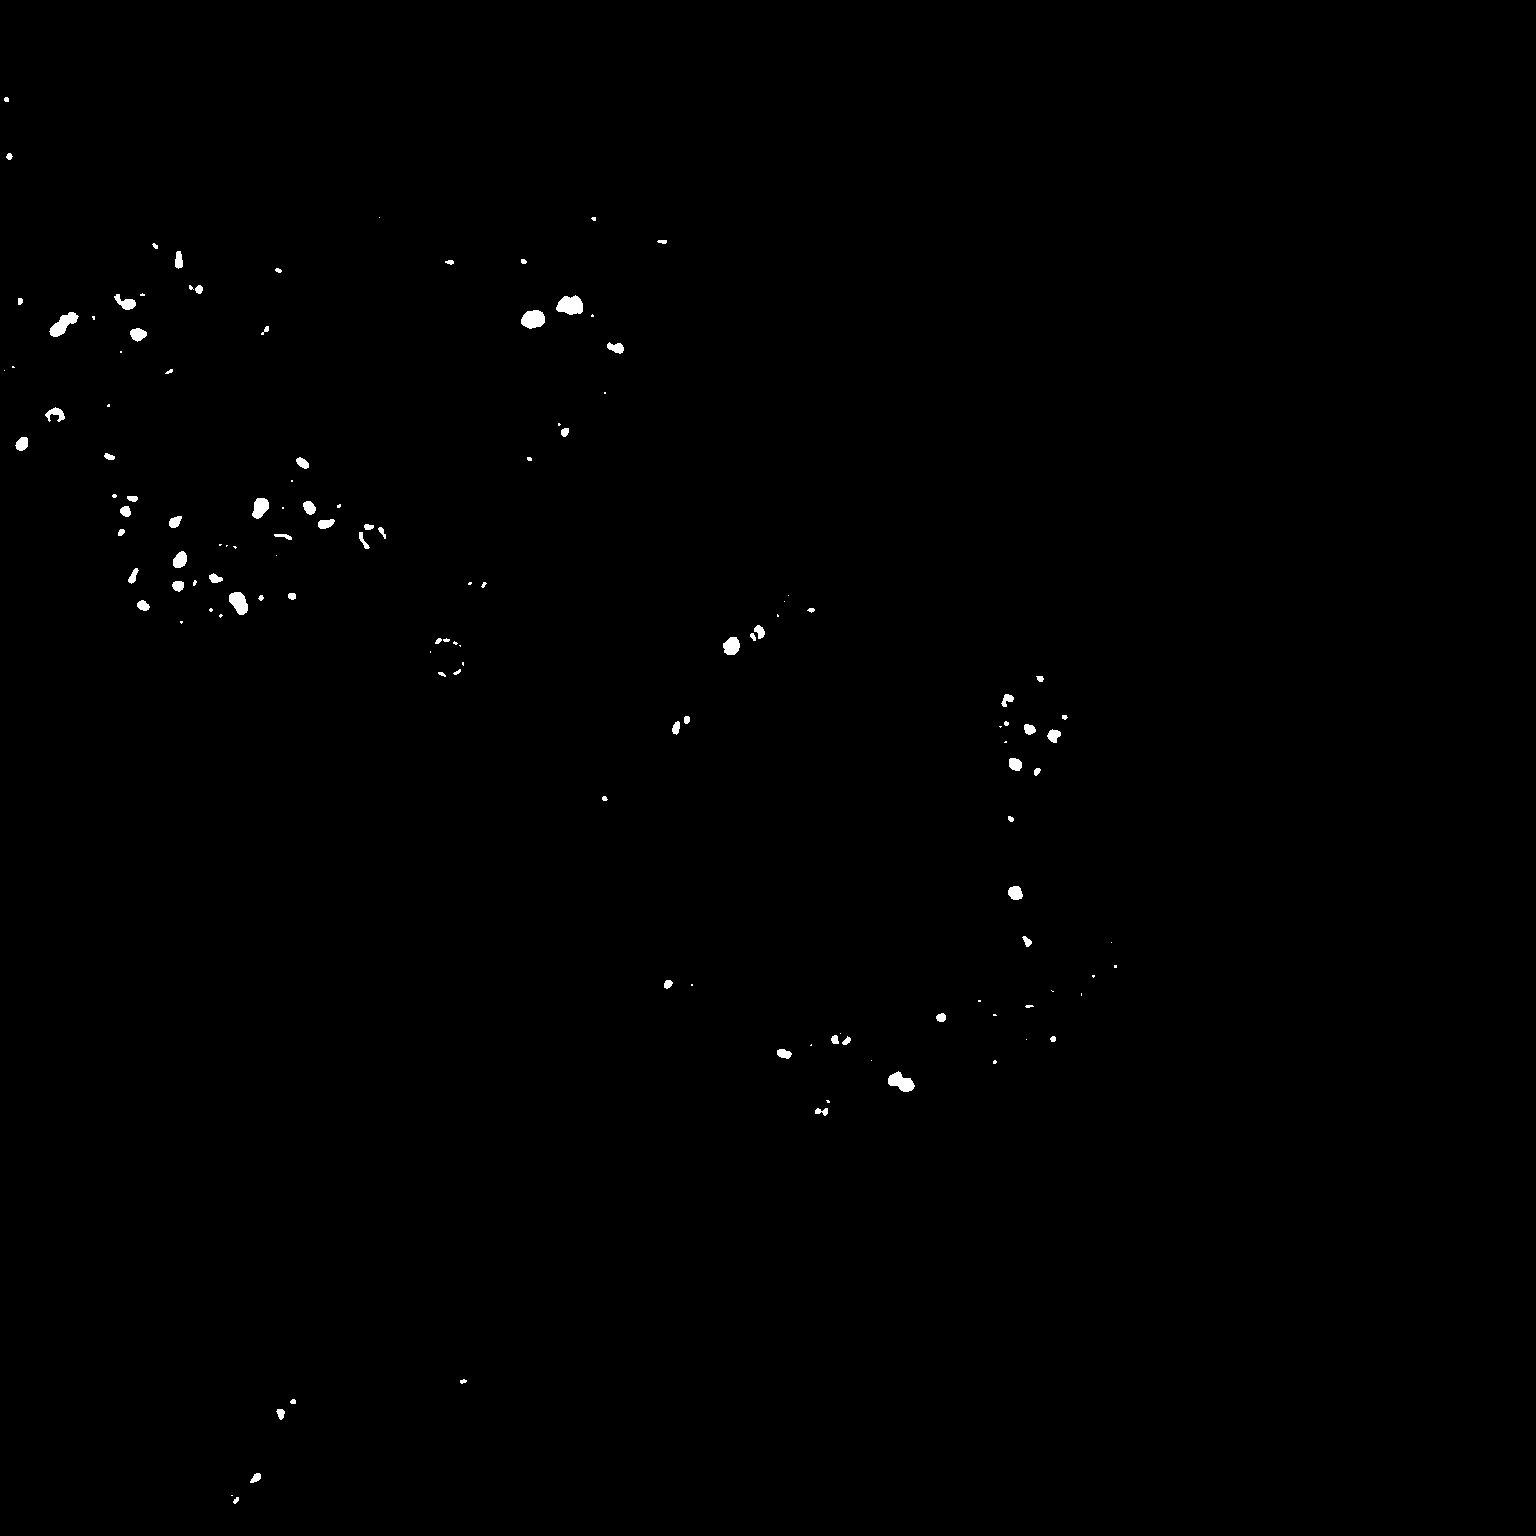
\includegraphics[width=0.2\textwidth]{figs/appendix/method_shortlisting/global_testing/Minimum_LML_4C=1.png}}
	\label{append-fig:Minimum_short}
	\caption{Minimum threshold outcomes for the shortlist sample images}
\end{figure}

\begin{figure}[ht!]
	\centering
	\subcaptionbox{Sample 1}{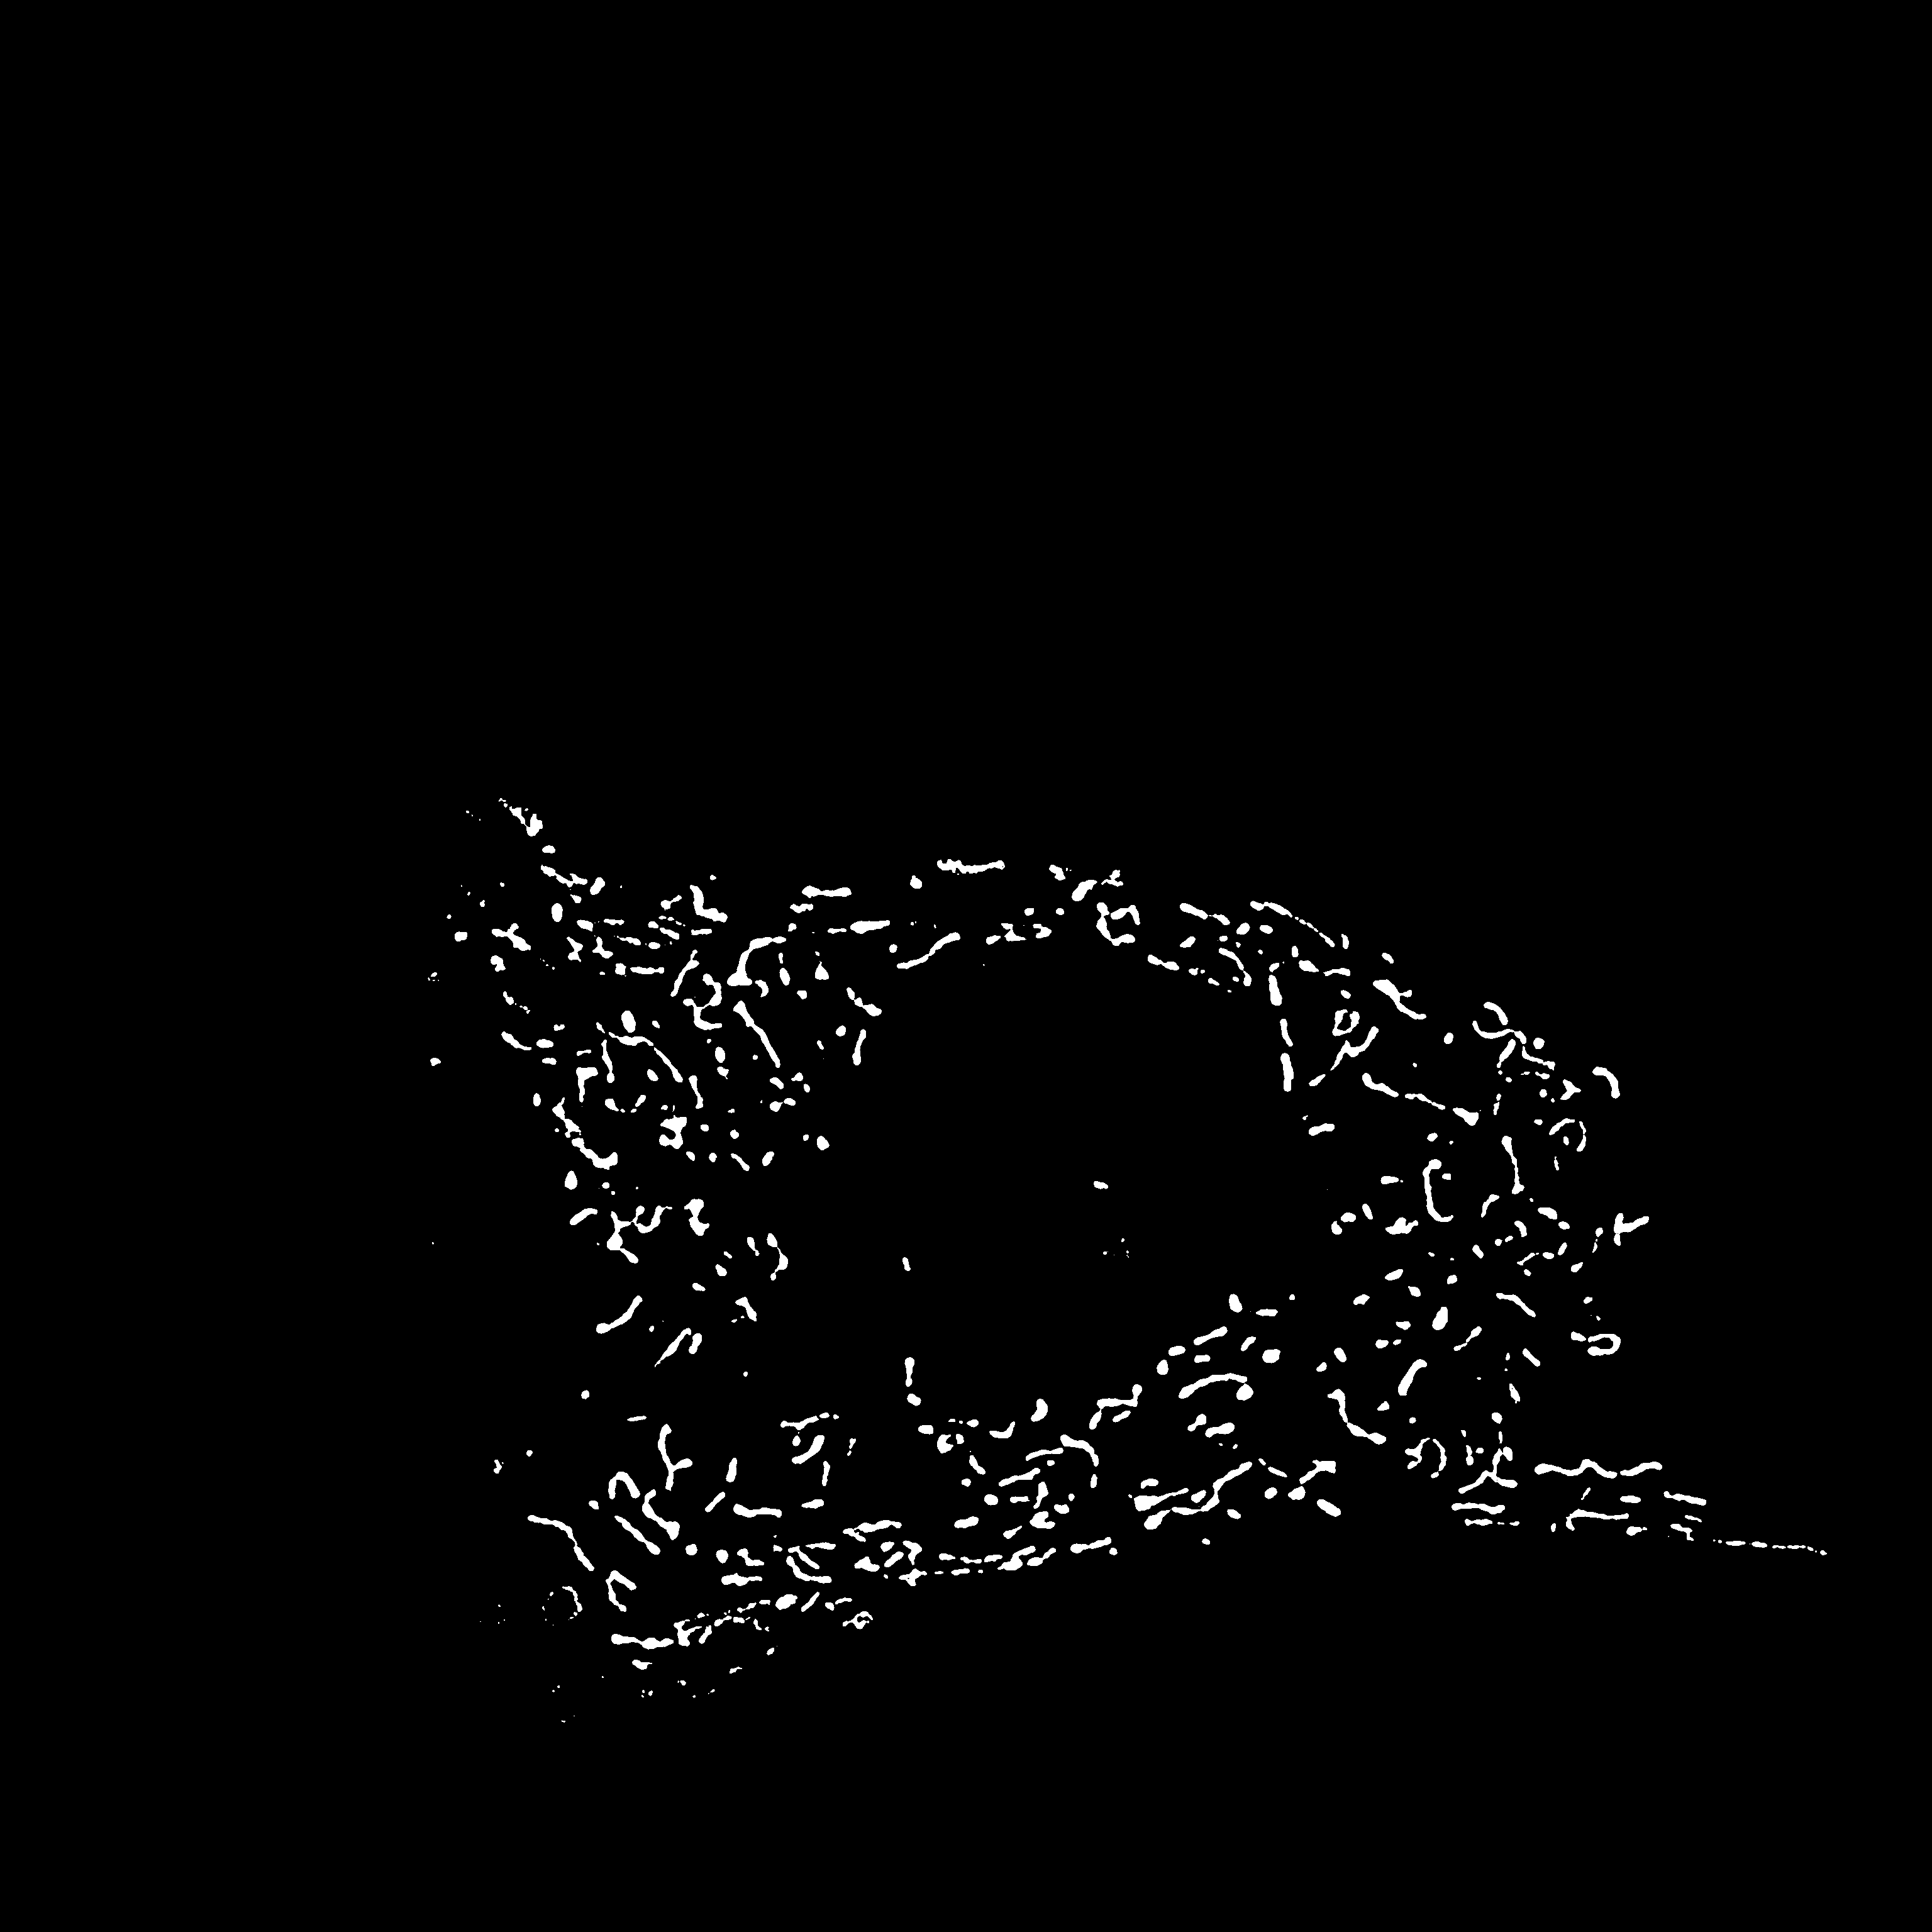
\includegraphics[width=0.2\textwidth]{figs/appendix/method_shortlisting/global_testing/Moments_CCCP_1C=1T=0.png}}
	\subcaptionbox{Sample 2}{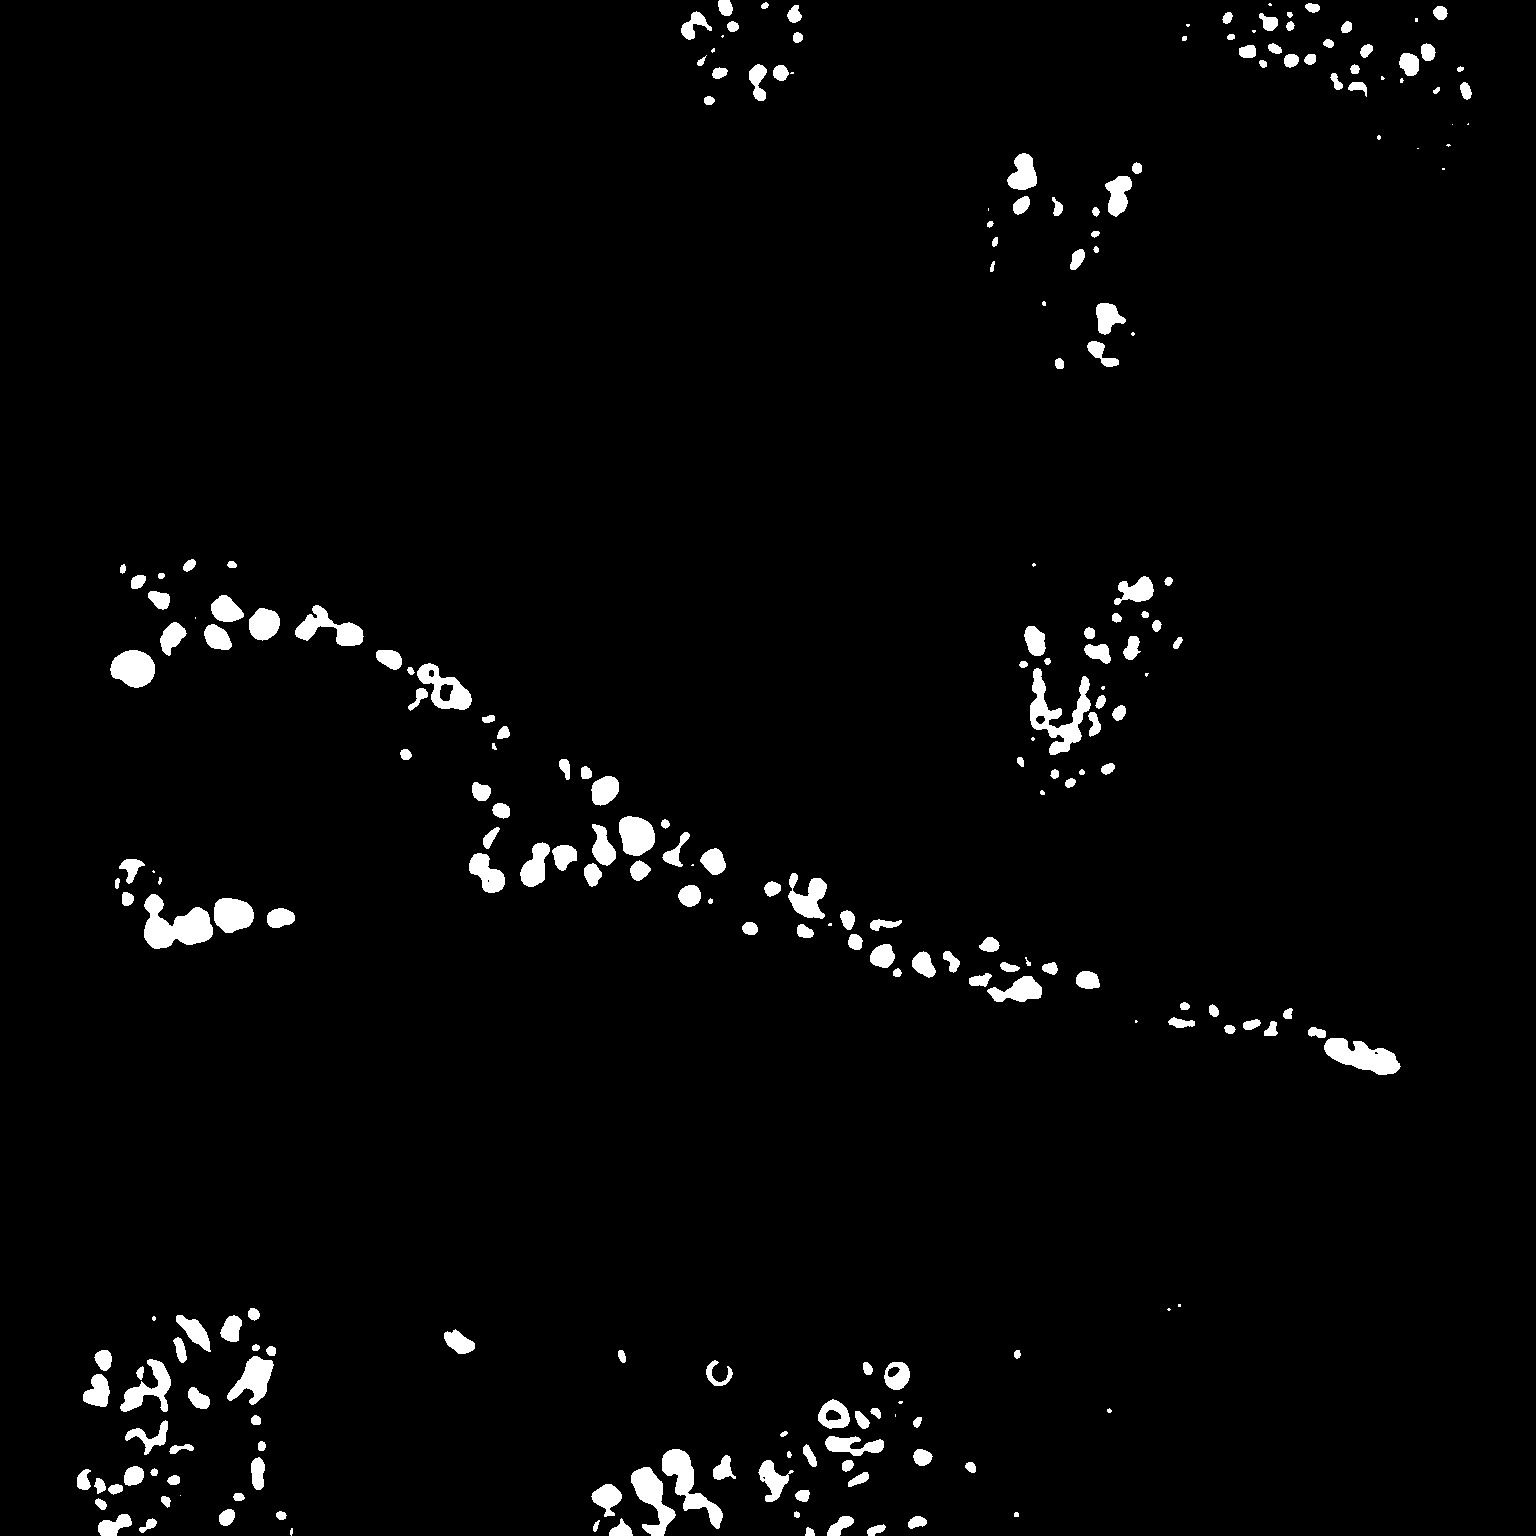
\includegraphics[width=0.2\textwidth]{figs/appendix/method_shortlisting/global_testing/Moments_HML_4C=0.png}}
	\subcaptionbox{Sample 3}{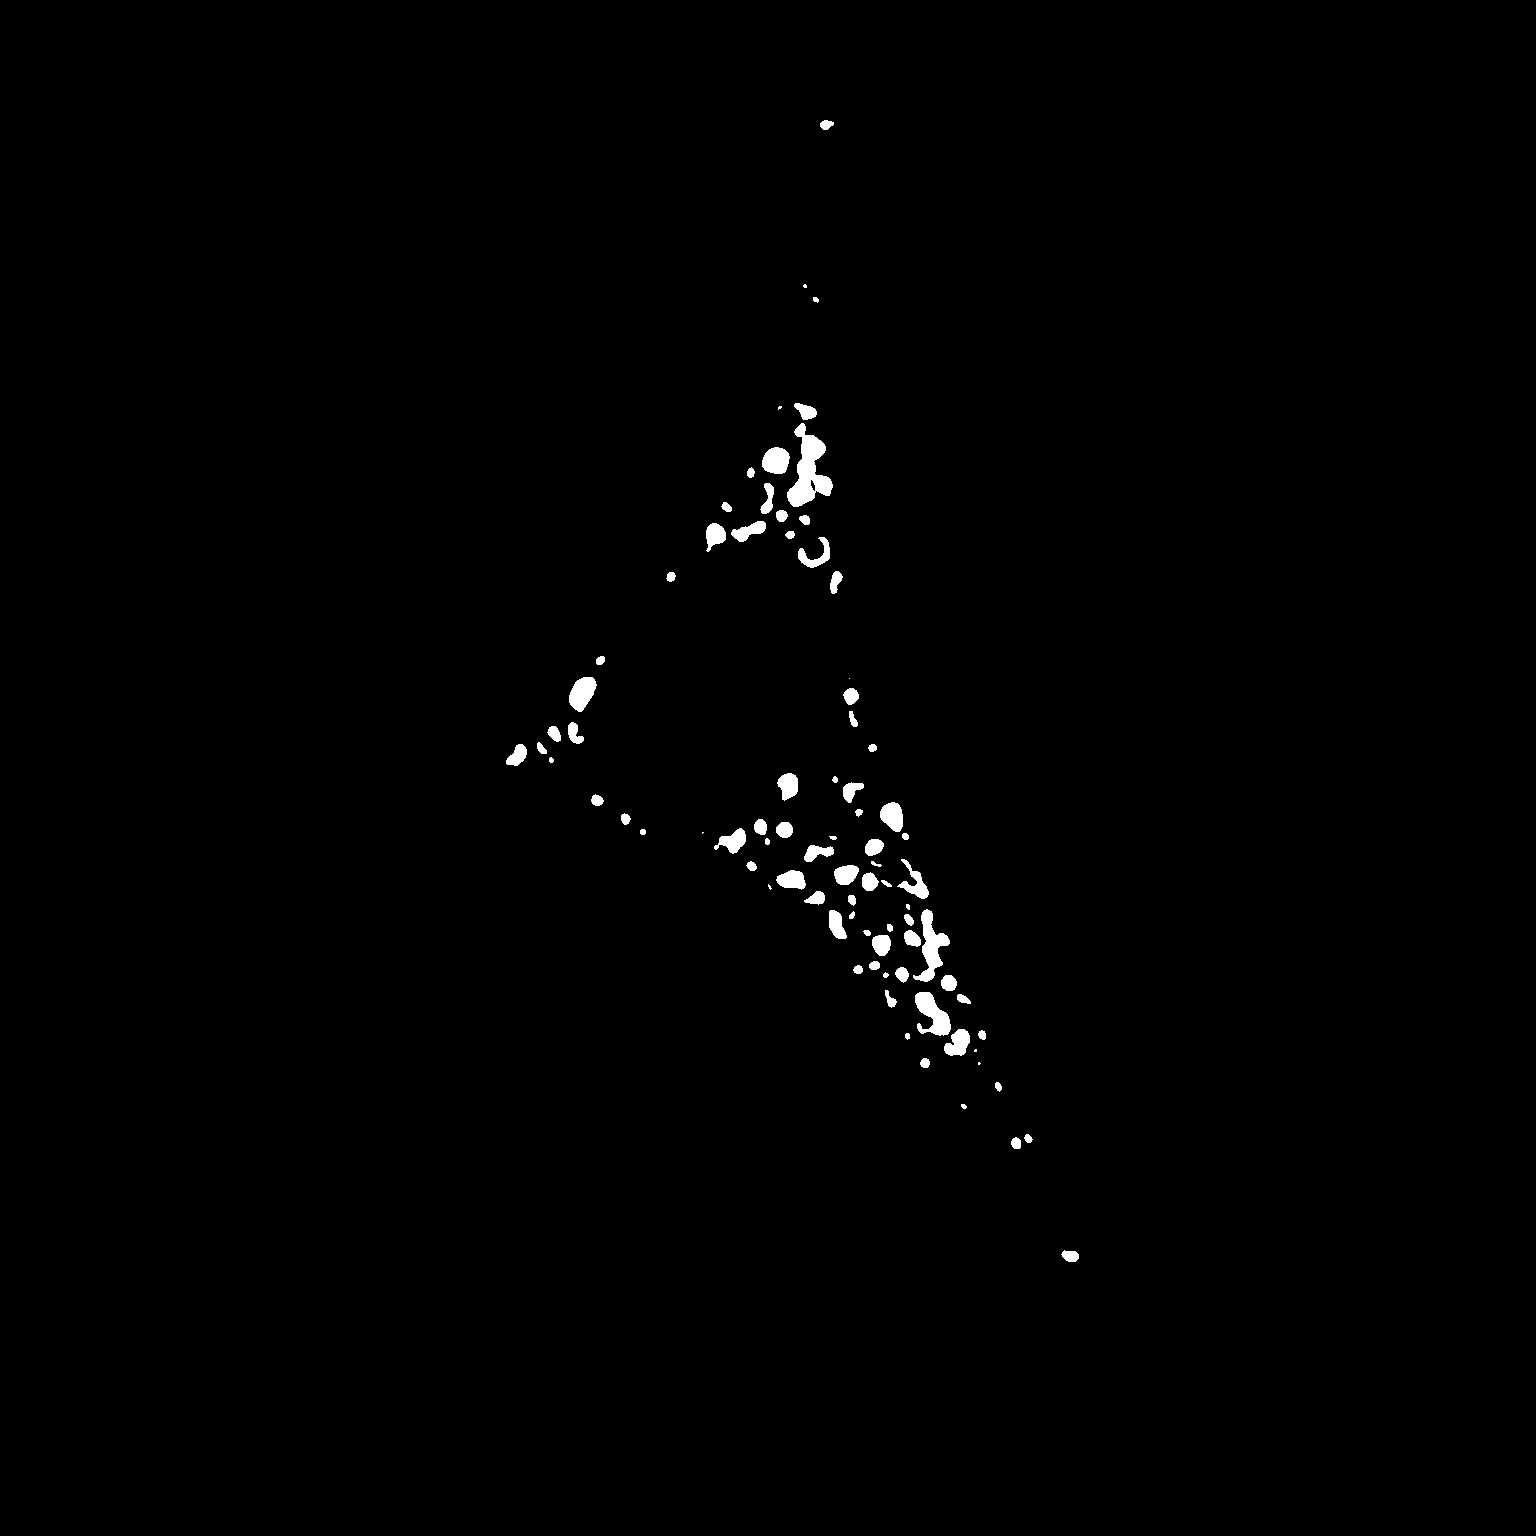
\includegraphics[width=0.2\textwidth]{figs/appendix/method_shortlisting/global_testing/Moments_LML_3C=0.png}}
	\subcaptionbox{Sample 4}{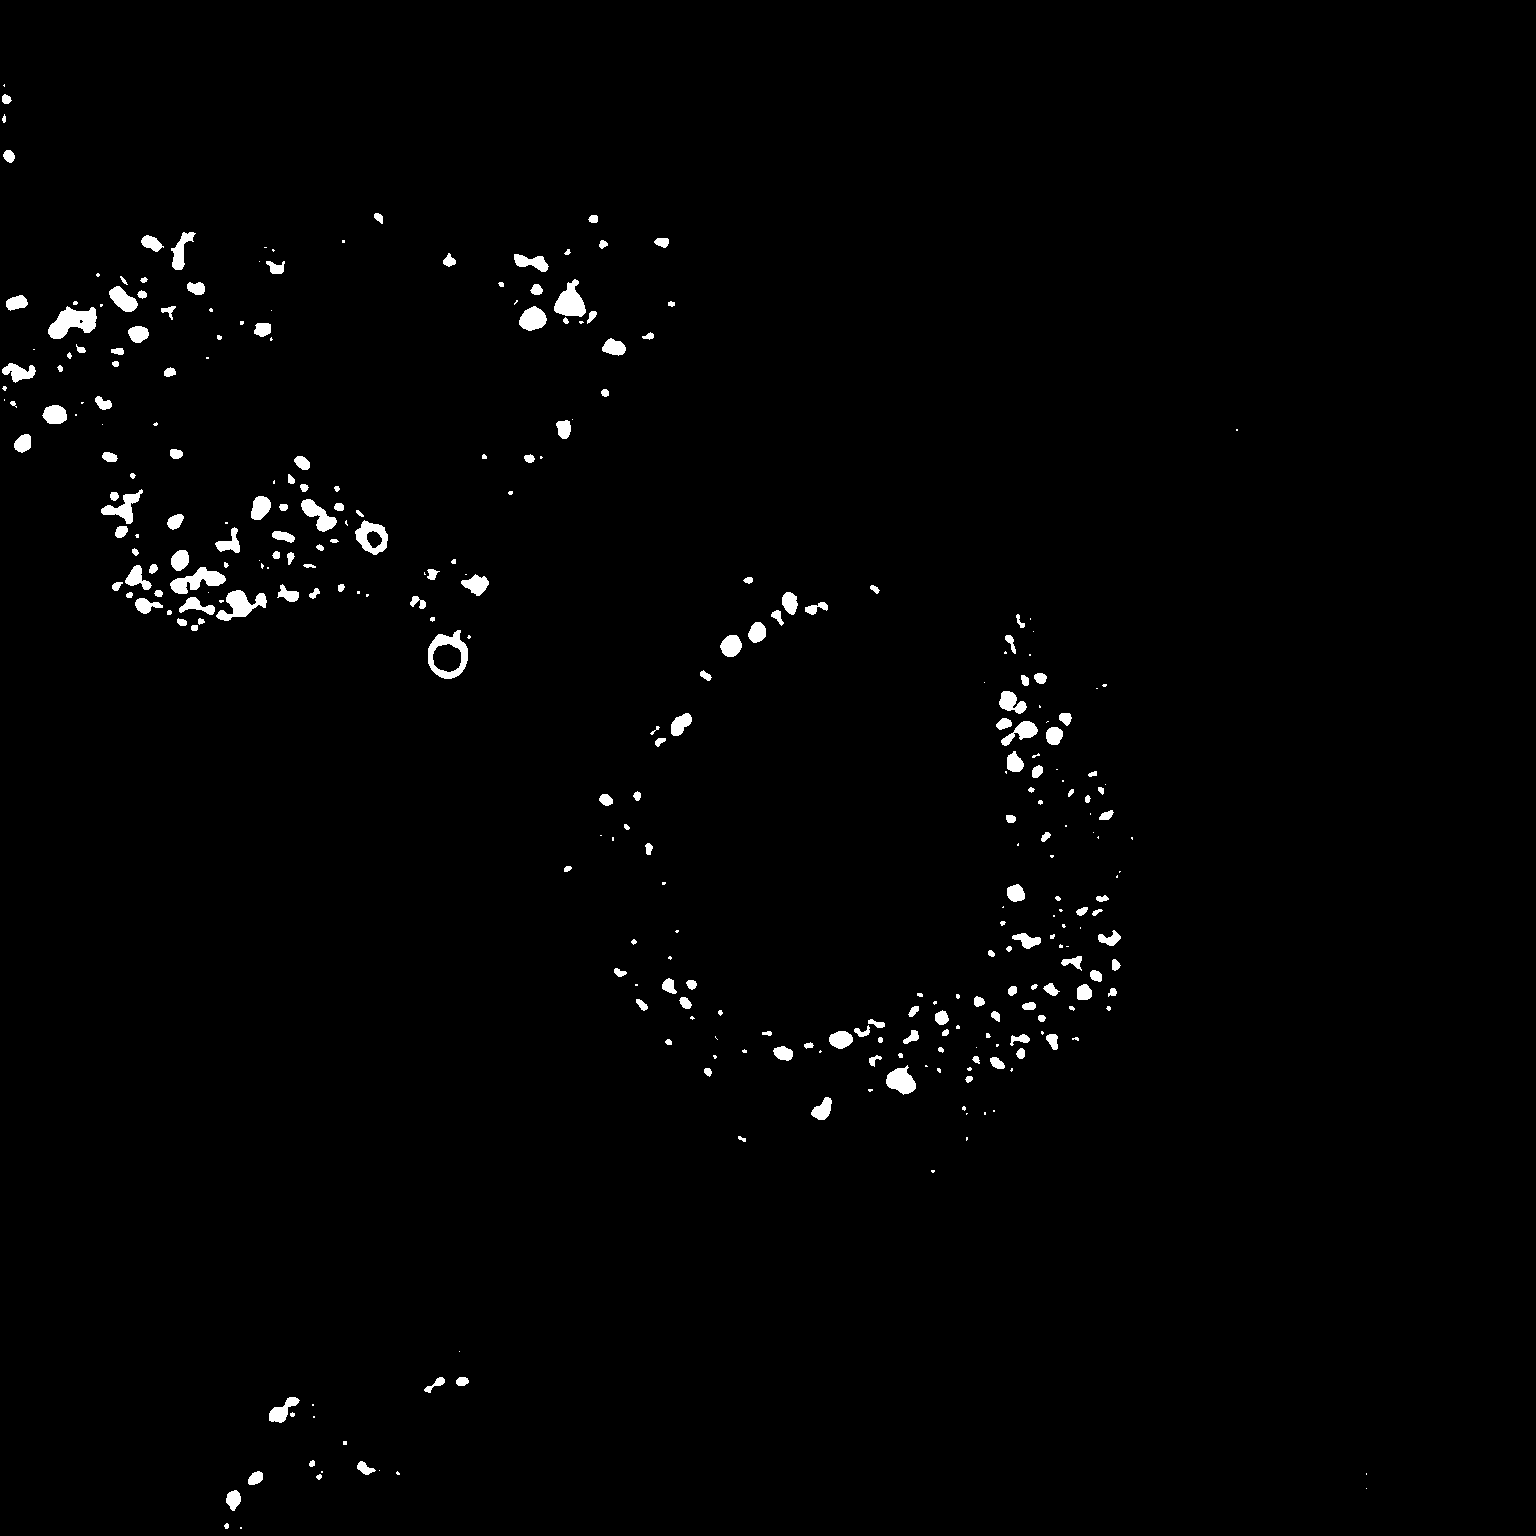
\includegraphics[width=0.2\textwidth]{figs/appendix/method_shortlisting/global_testing/Moments_LML_4C=1.png}}
	\label{append-fig:Moments_short}
	\caption{Moments threshold outcomes for the shortlist sample images}
\end{figure}

\begin{figure}[ht!]
	\centering
	\subcaptionbox{Sample 1}{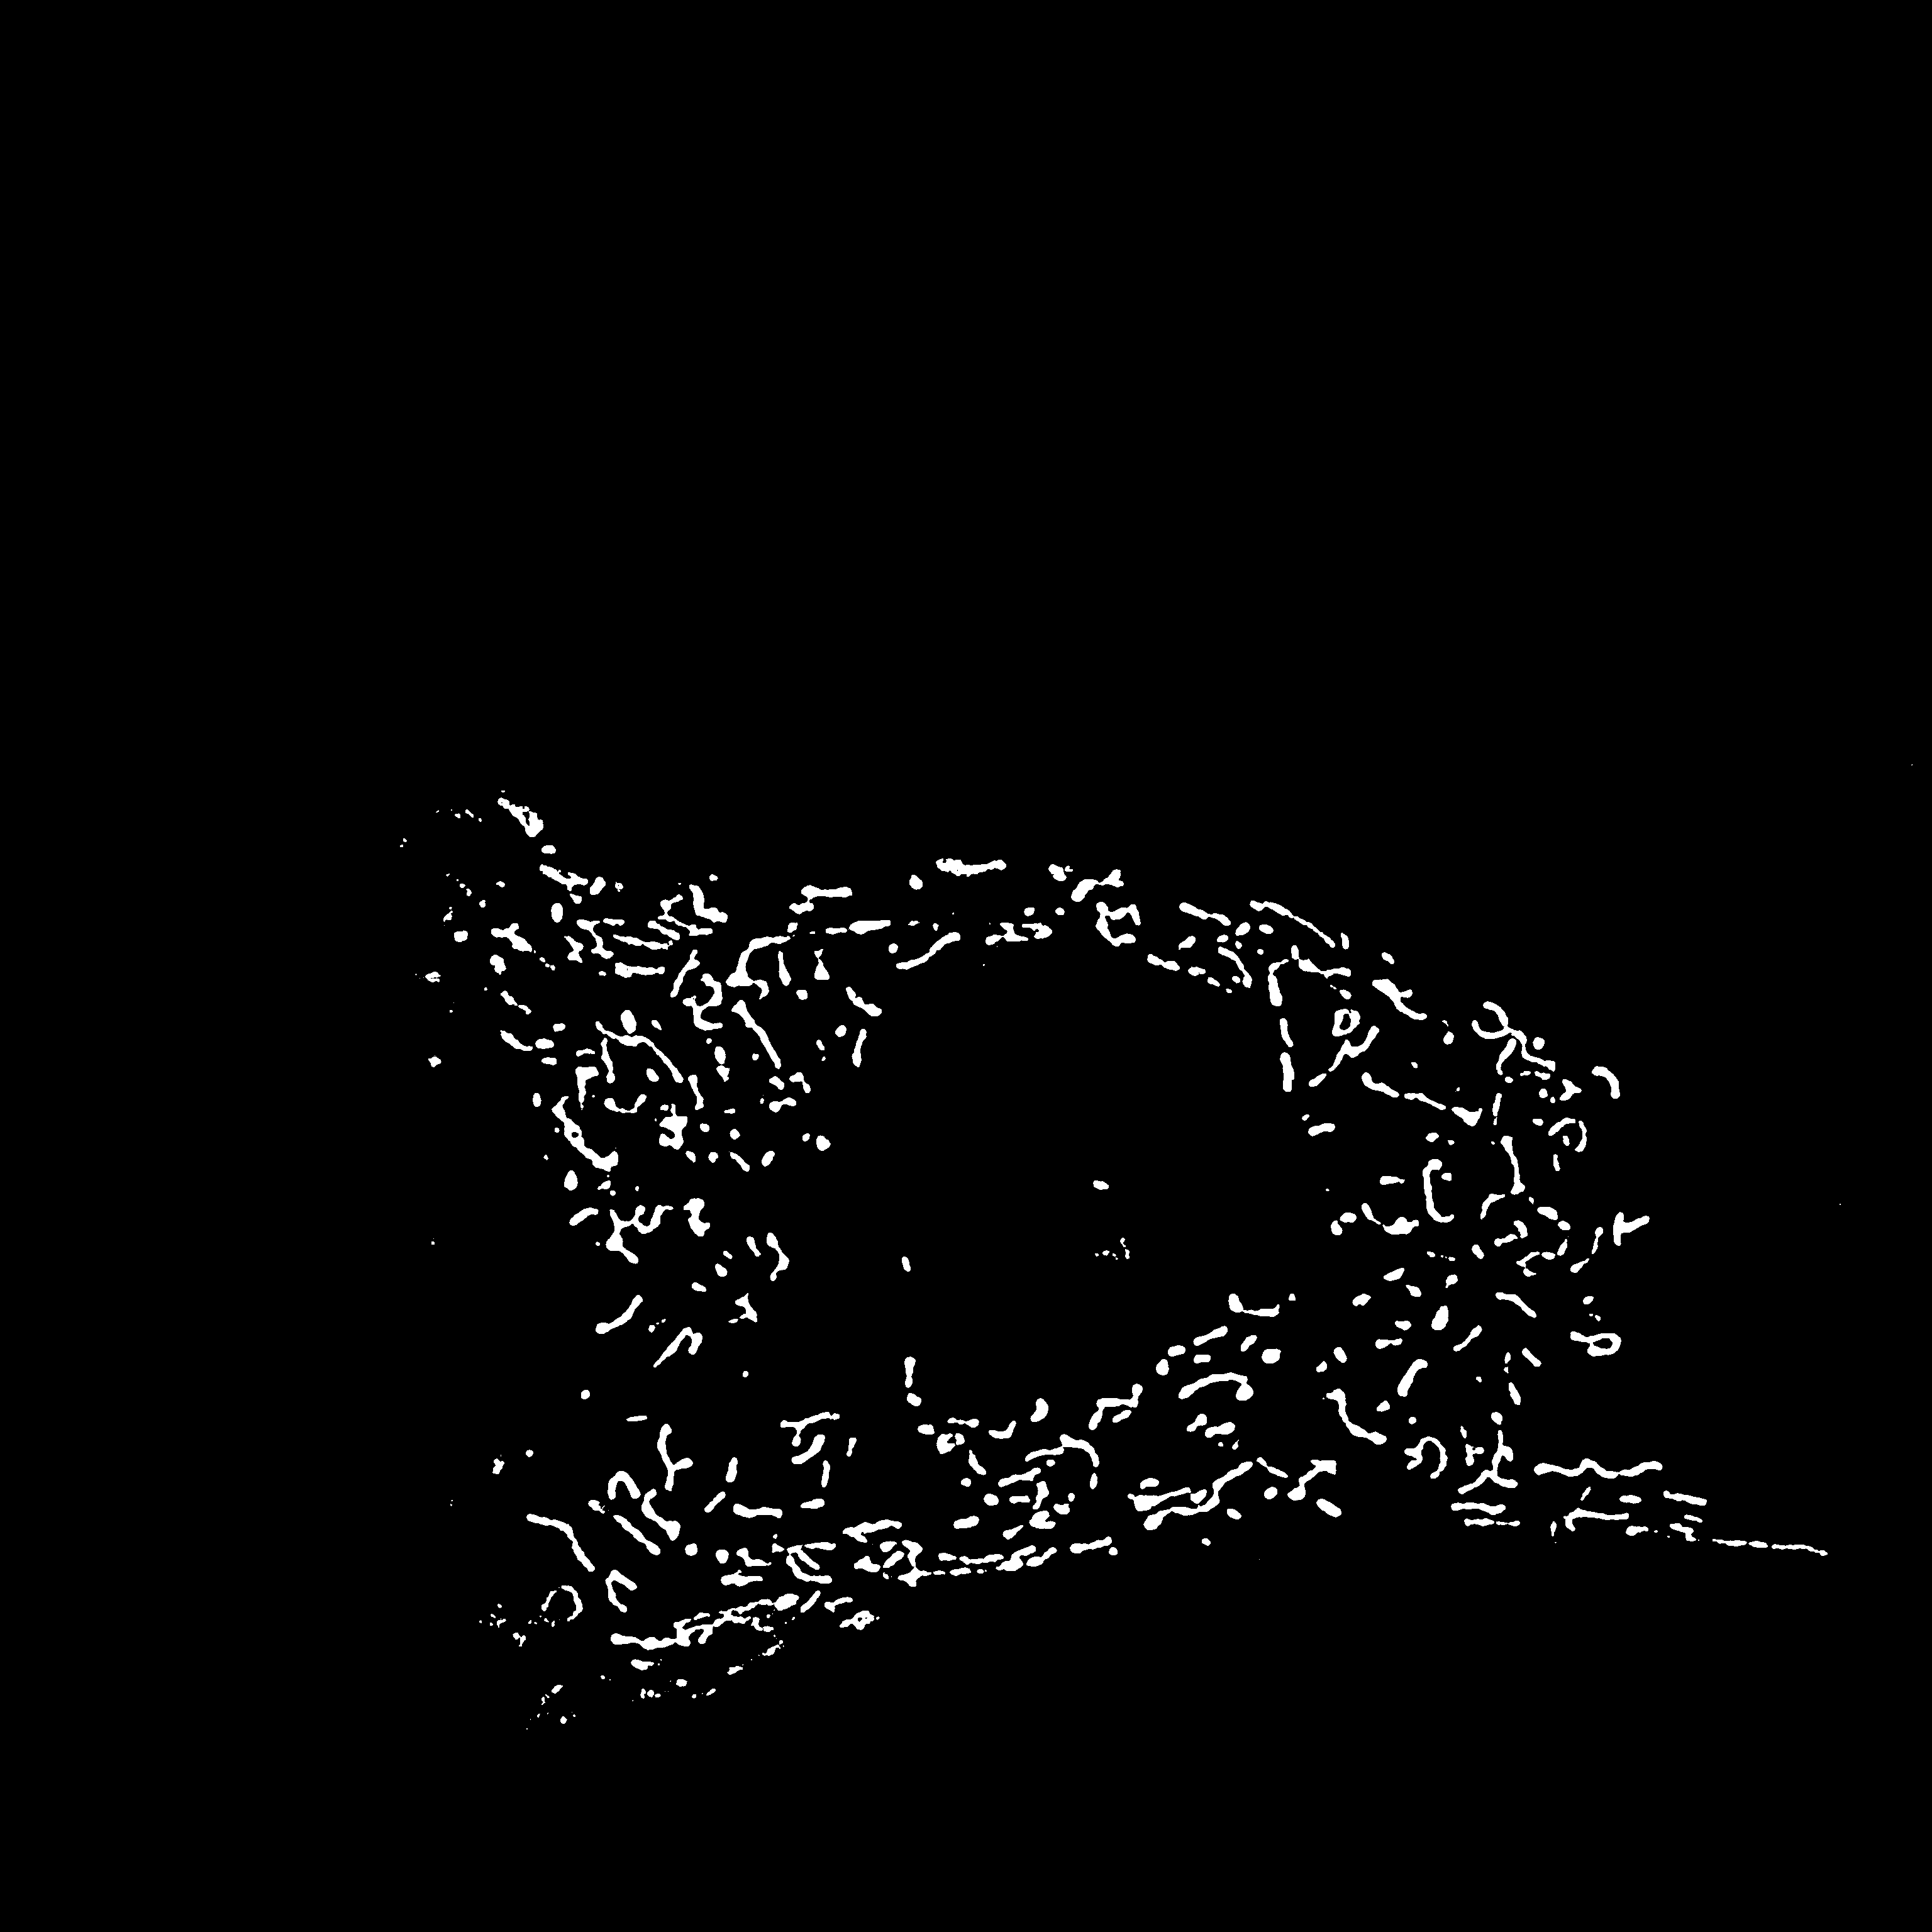
\includegraphics[width=0.2\textwidth]{figs/appendix/method_shortlisting/global_testing/Otsu_CCCP_1C=1T=0.png}}
	\subcaptionbox{Sample 2}{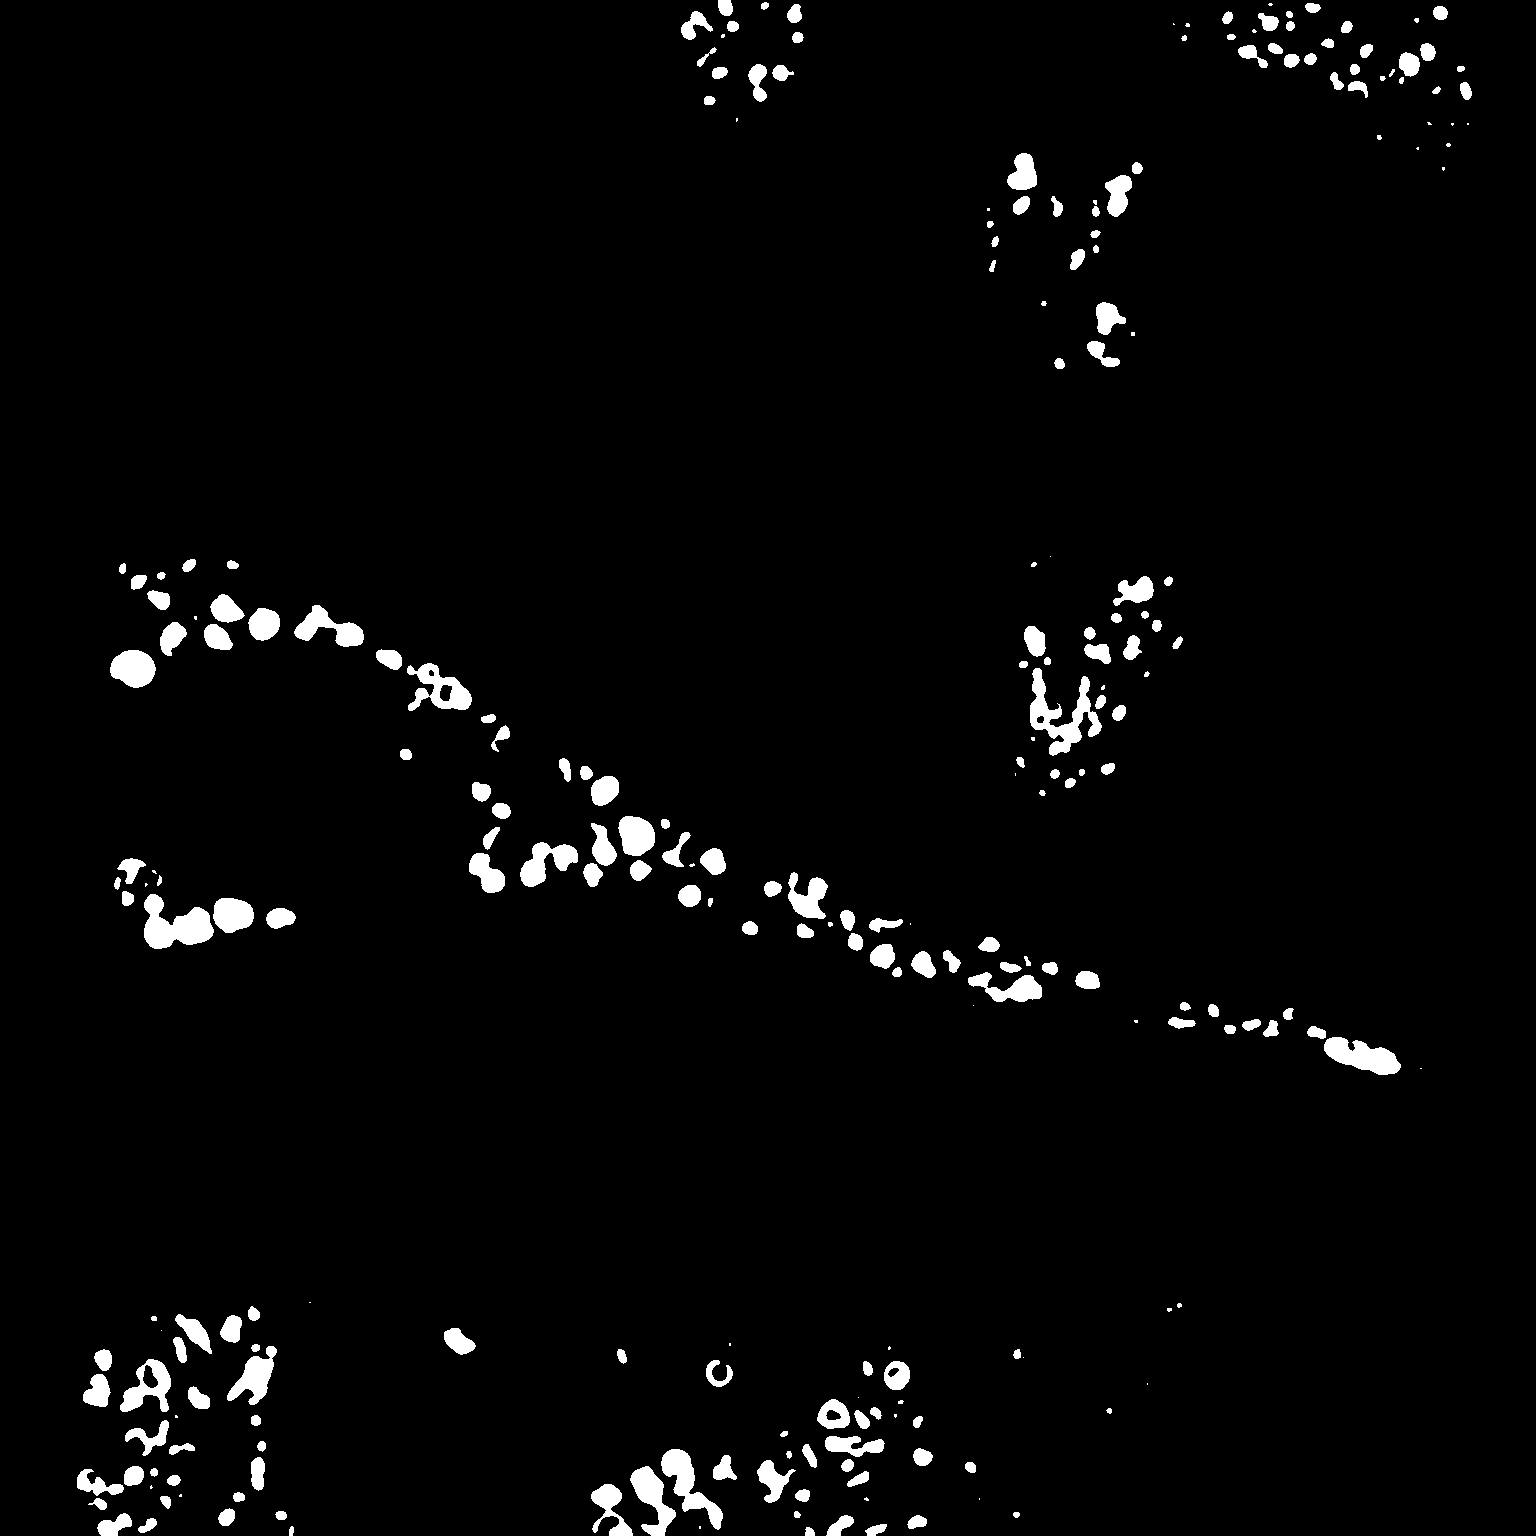
\includegraphics[width=0.2\textwidth]{figs/appendix/method_shortlisting/global_testing/Otsu_HML_4C=0.png}}
	\subcaptionbox{Sample 3}{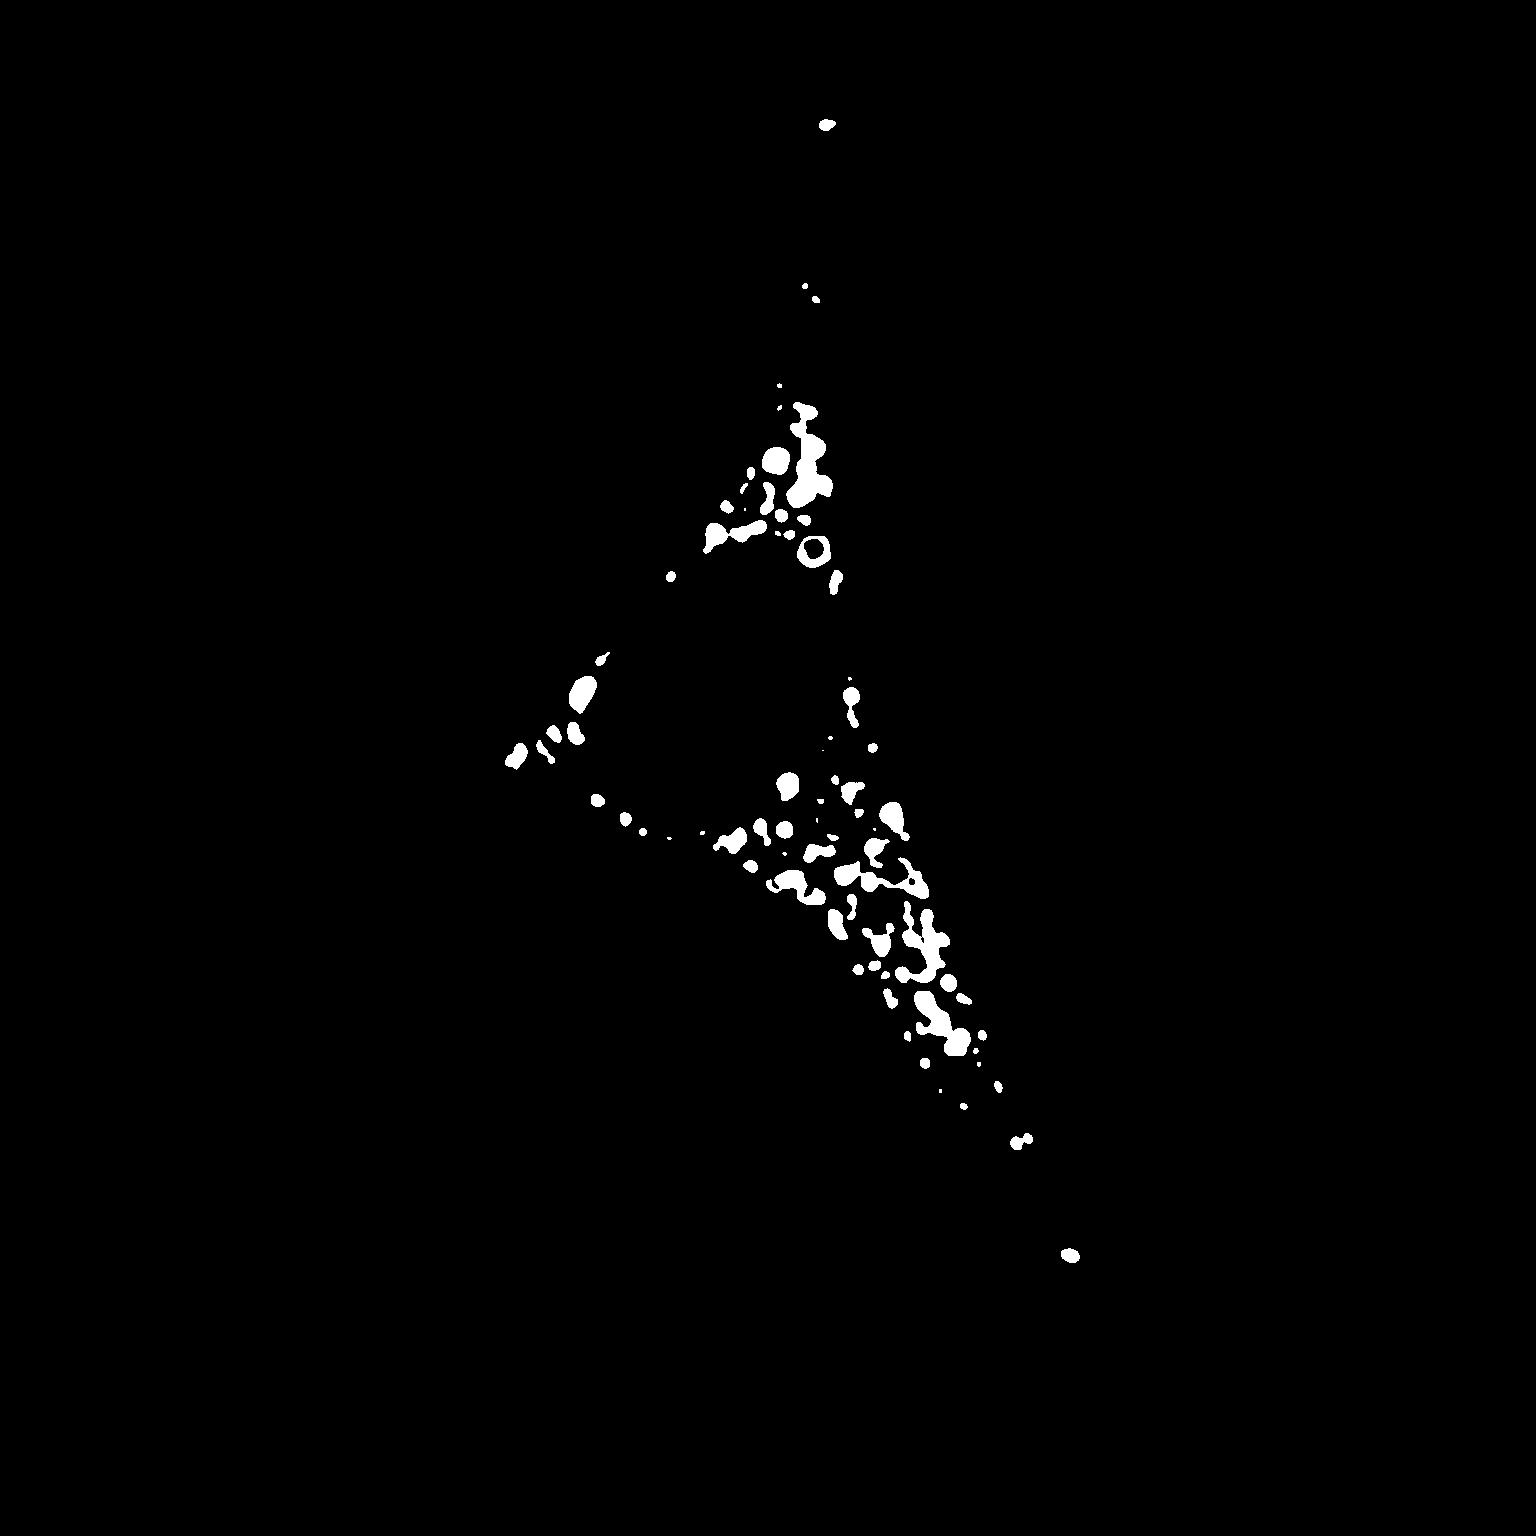
\includegraphics[width=0.2\textwidth]{figs/appendix/method_shortlisting/global_testing/Otsu_LML_3C=0.png}}
	\subcaptionbox{Sample 4}{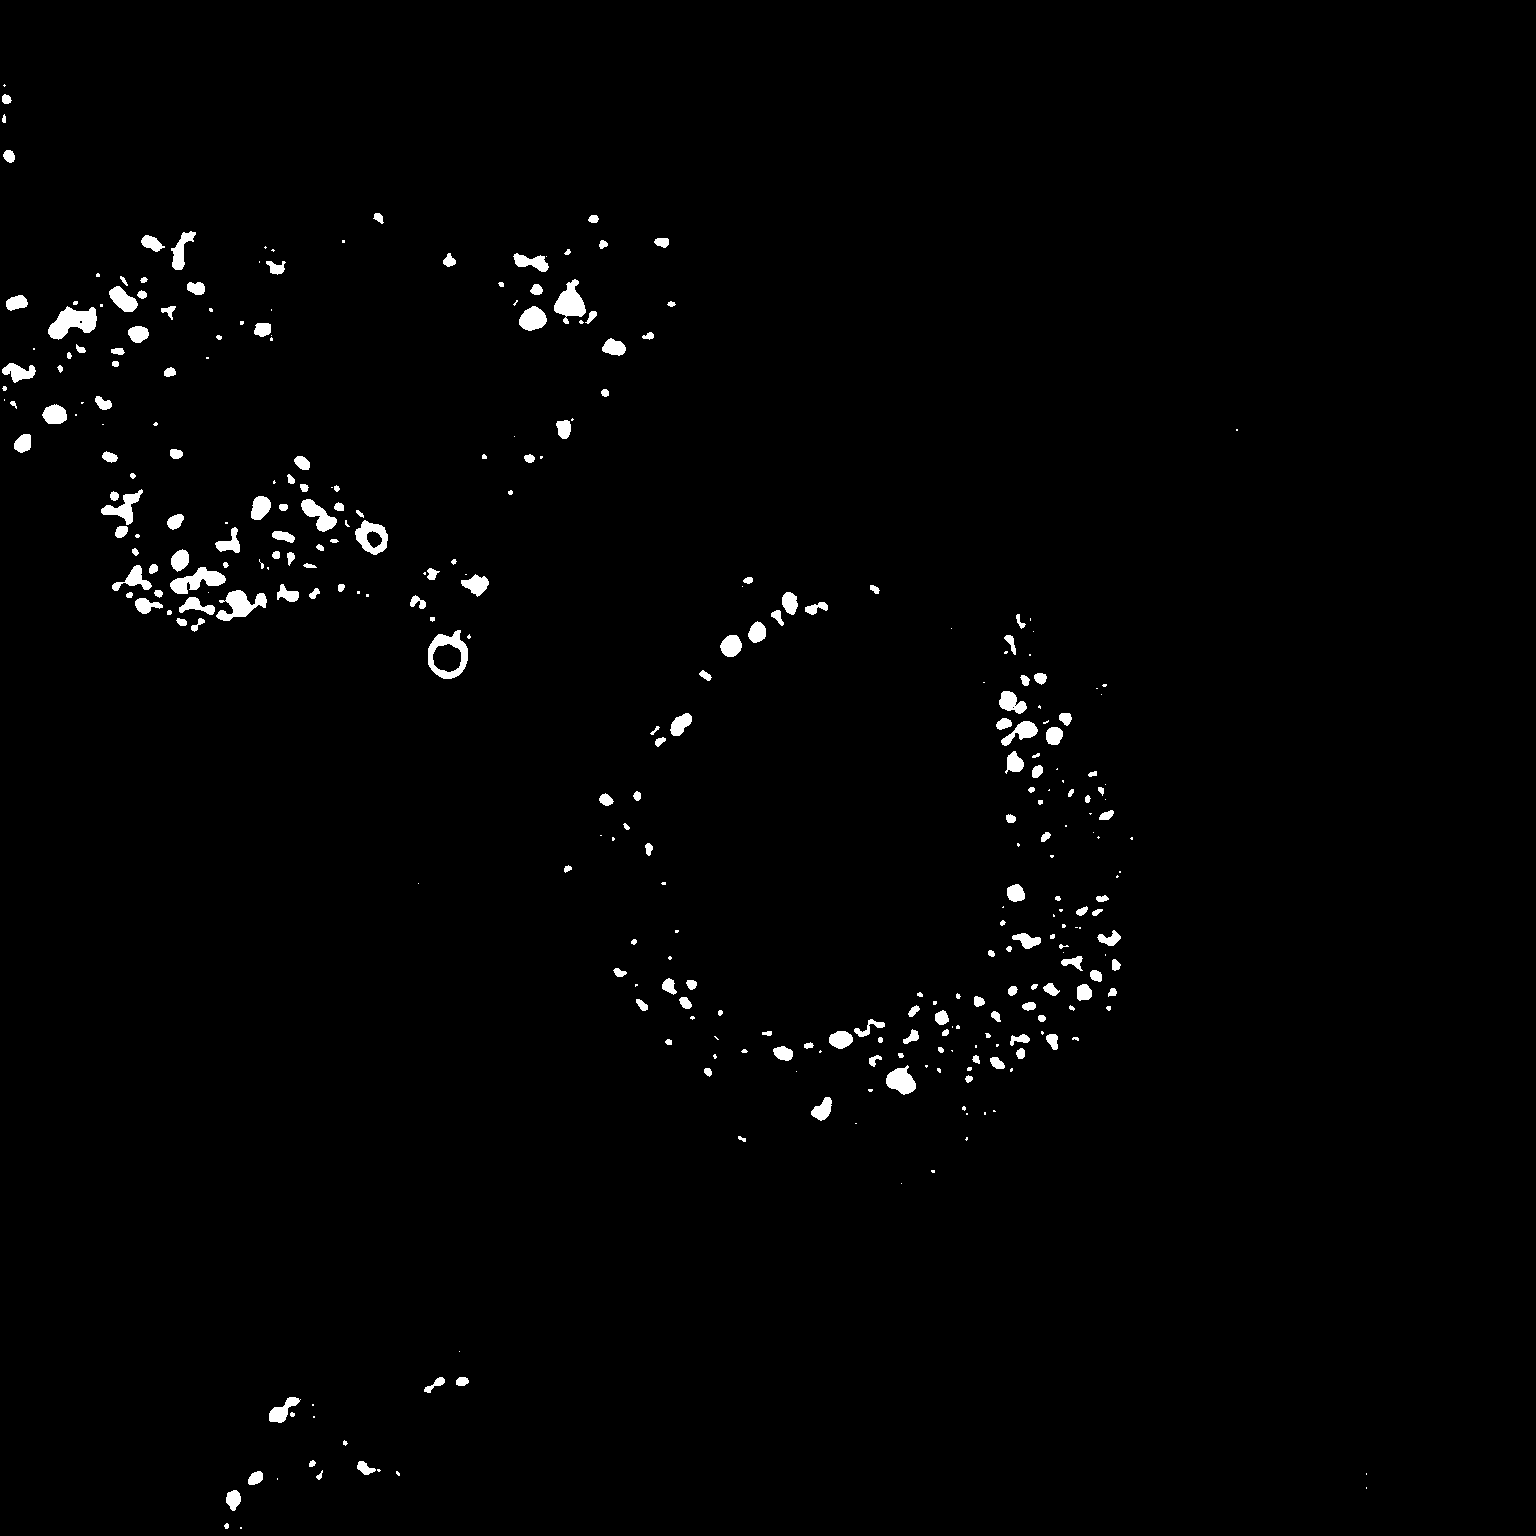
\includegraphics[width=0.2\textwidth]{figs/appendix/method_shortlisting/global_testing/Otsu_LML_4C=1.png}}
	\label{append-fig:Otsu_short}
	\caption{Otsu threshold outcomes for the shortlist sample images}
\end{figure}

\begin{figure}[ht!]
	\centering
	\subcaptionbox{Sample 1}{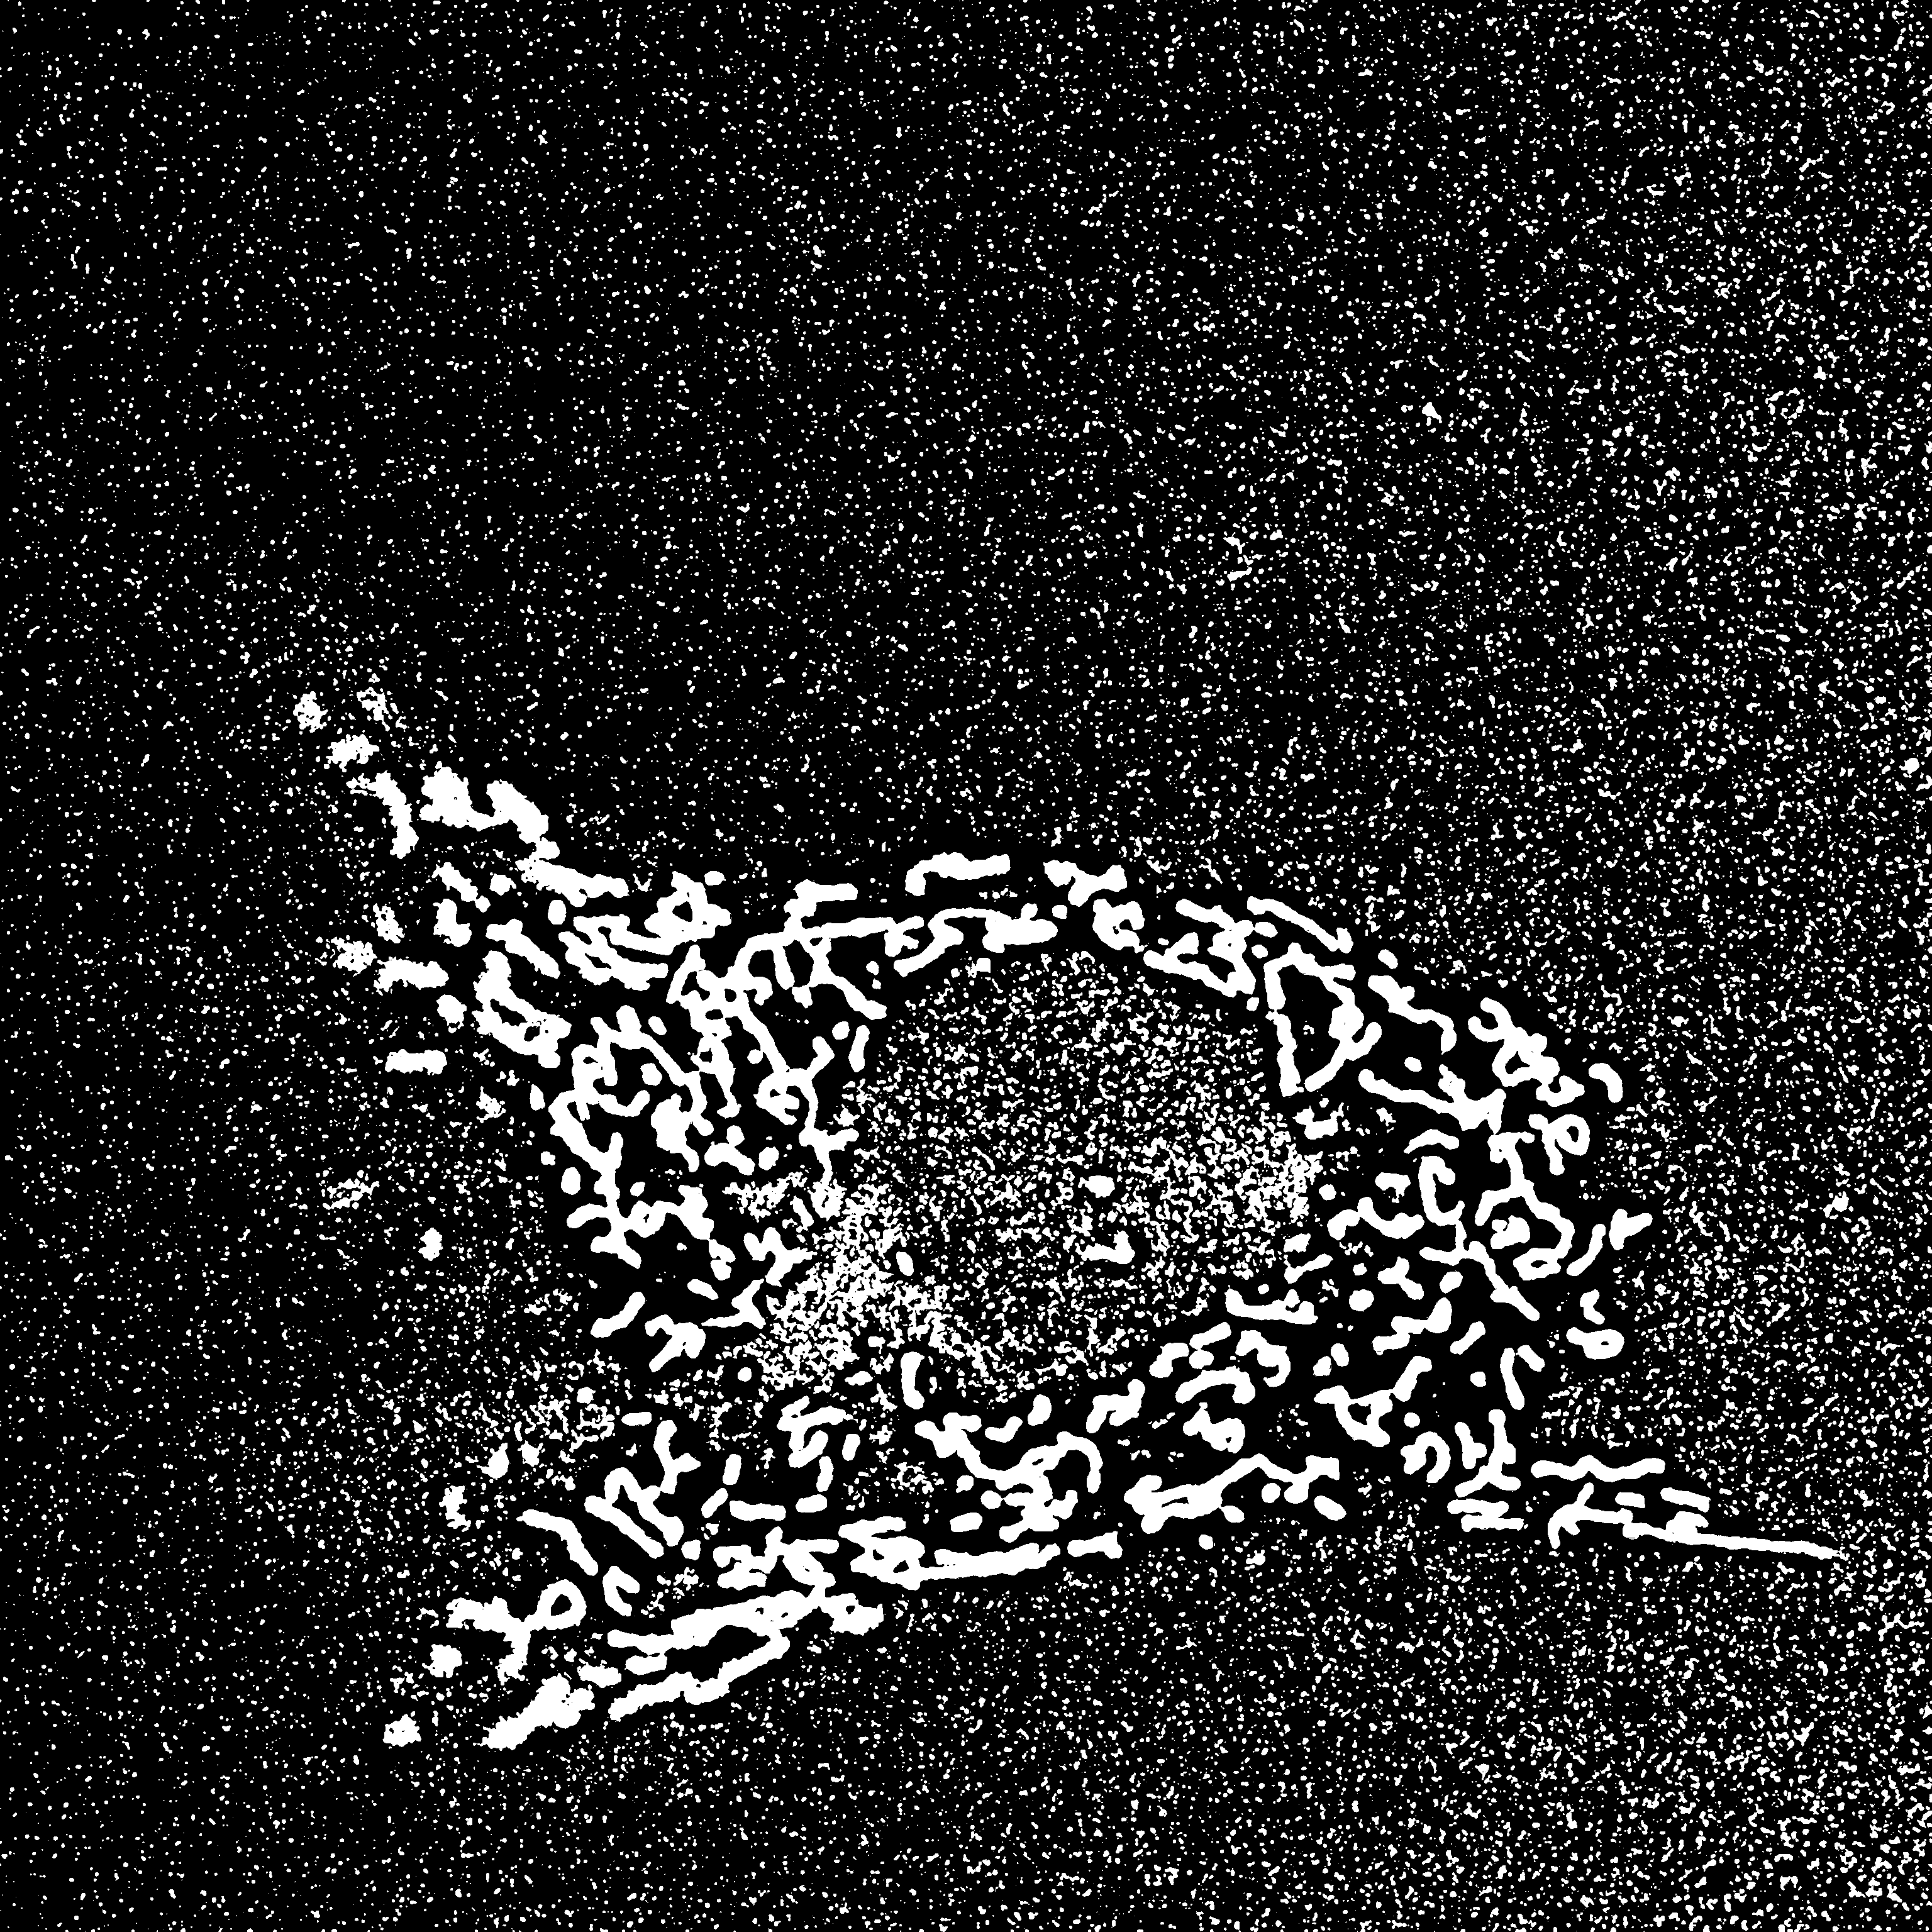
\includegraphics[width=0.2\textwidth]{figs/appendix/method_shortlisting/global_testing/Percentile_CCCP_1C=1T=0.png}}
	\subcaptionbox{Sample 2}{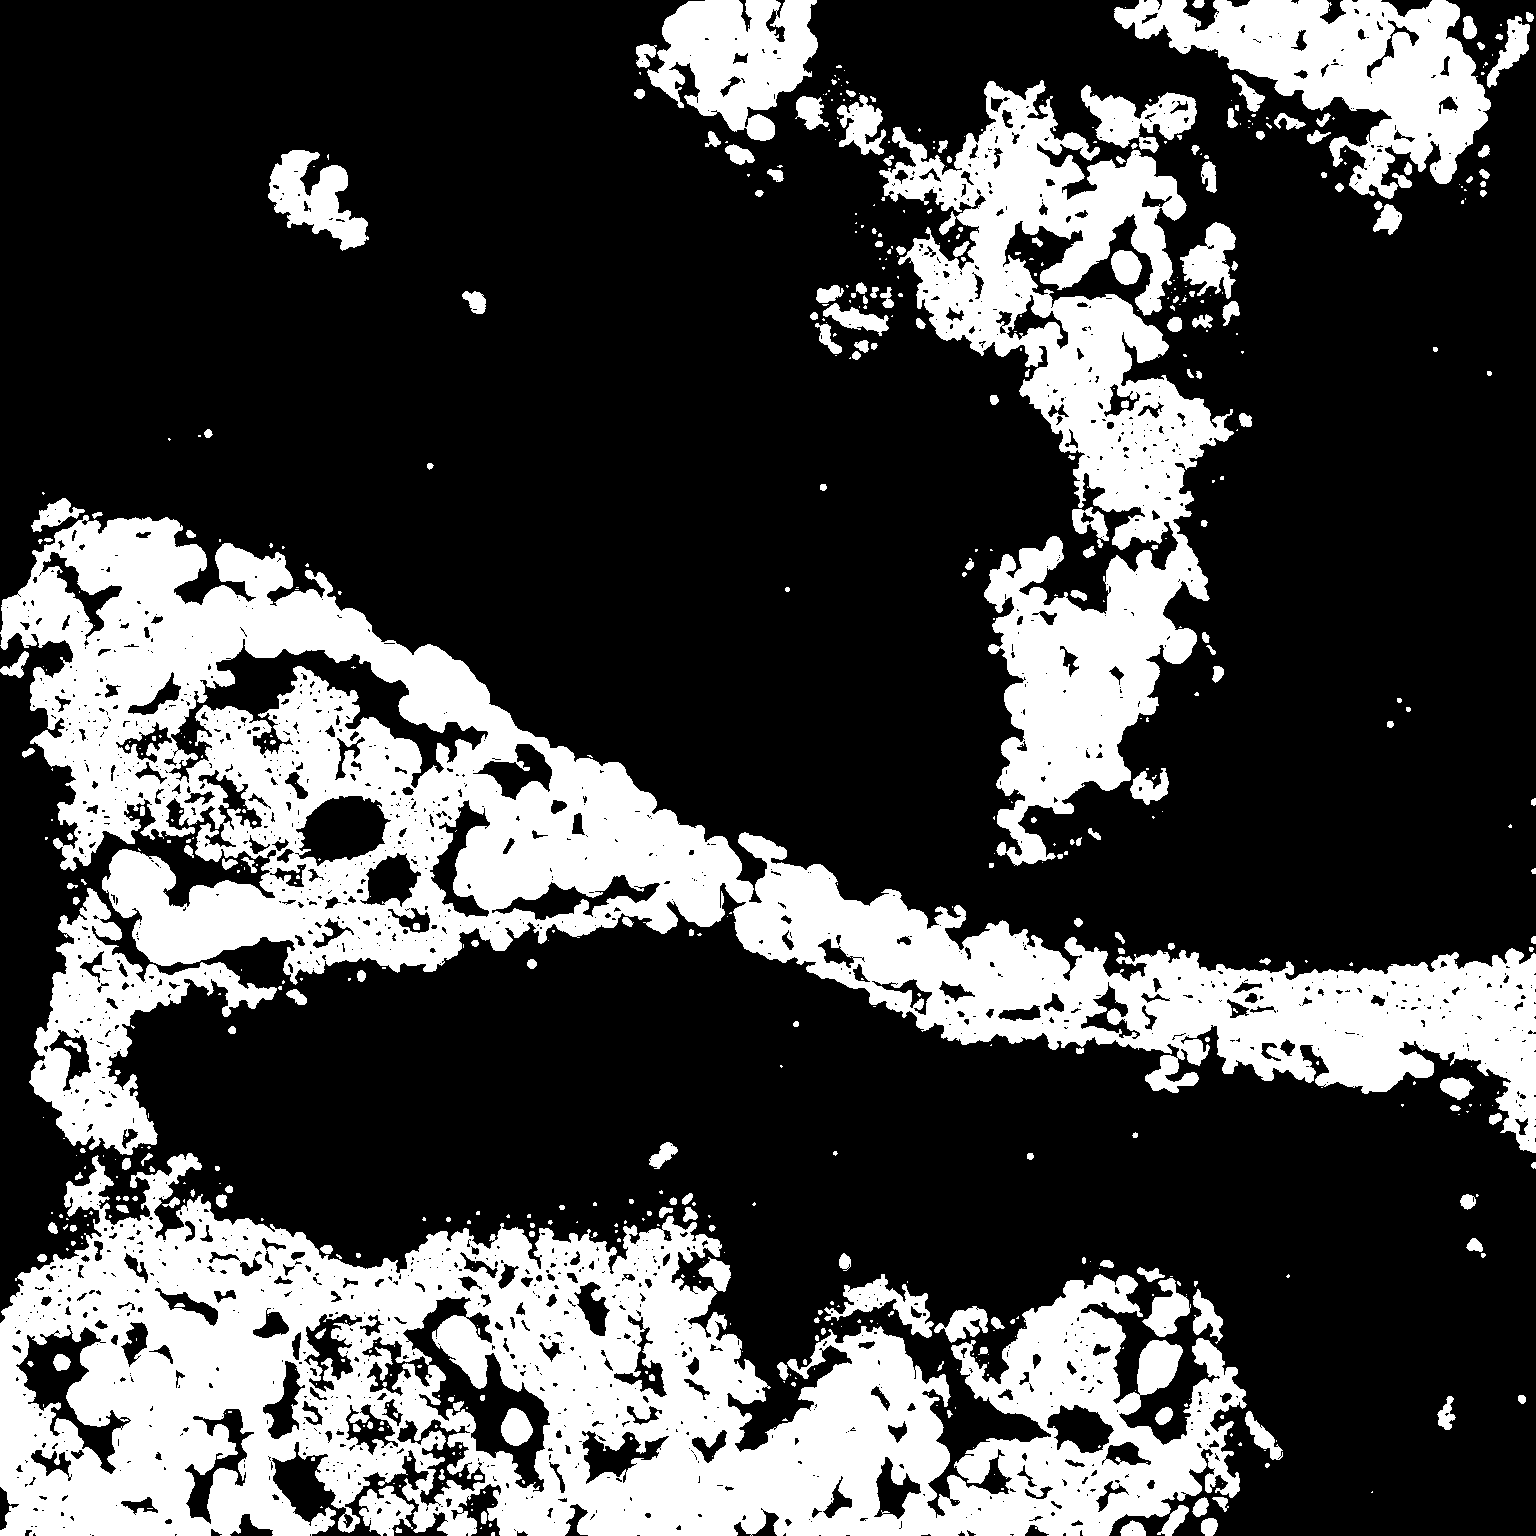
\includegraphics[width=0.2\textwidth]{figs/appendix/method_shortlisting/global_testing/Percentile_HML_4C=0.png}}
	\subcaptionbox{Sample 3}{\includegraphics[width=0.2\textwidth]{figs/appendix/method_shortlisting/global_testing/Percentile_LML_3C=0.png}}
	\subcaptionbox{Sample 4}{\includegraphics[width=0.2\textwidth]{figs/appendix/method_shortlisting/global_testing/Percentile_LML_4C=1.png}}
	\label{append-fig:Percentile_short}
	\caption{Percentile threshold outcomes for the shortlist sample images}
\end{figure}

\begin{figure}[ht!]
	\centering
	\subcaptionbox{Sample 1}{\includegraphics[width=0.2\textwidth]{figs/appendix/method_shortlisting/global_testing/RenyiEntropy_CCCP_1C=1T=0.png}}
	\subcaptionbox{Sample 2}{\includegraphics[width=0.2\textwidth]{figs/appendix/method_shortlisting/global_testing/RenyiEntropy_HML_4C=0.png}}
	\subcaptionbox{Sample 3}{\includegraphics[width=0.2\textwidth]{figs/appendix/method_shortlisting/global_testing/RenyiEntropy_LML_3C=0.png}}
	\subcaptionbox{Sample 4}{\includegraphics[width=0.2\textwidth]{figs/appendix/method_shortlisting/global_testing/RenyiEntropy_LML_4C=1.png}}
	\label{append-fig:RenyiEntropy_short}
	\caption{RenyiEntropy threshold outcomes for the shortlist sample images}
\end{figure}

\begin{figure}[ht!]
	\centering
	\subcaptionbox{Sample 1}{\includegraphics[width=0.2\textwidth]{figs/appendix/method_shortlisting/global_testing/Shanbhag_CCCP_1C=1T=0.png}}
	\subcaptionbox{Sample 2}{\includegraphics[width=0.2\textwidth]{figs/appendix/method_shortlisting/global_testing/Shanbhag_HML_4C=0.png}}
	\subcaptionbox{Sample 3}{\includegraphics[width=0.2\textwidth]{figs/appendix/method_shortlisting/global_testing/Shanbhag_LML_3C=0.png}}
	\subcaptionbox{Sample 4}{\includegraphics[width=0.2\textwidth]{figs/appendix/method_shortlisting/global_testing/Shanbhag_LML_4C=1.png}}
	\label{append-fig:Shanbhag_short}
	\caption{Shanbhag threshold outcomes for the shortlist sample images}
\end{figure}

\begin{figure}[ht!]
	\centering
	\subcaptionbox{Sample 1}{\includegraphics[width=0.2\textwidth]{figs/appendix/method_shortlisting/global_testing/Triangle_CCCP_1C=1T=0.png}}
	\subcaptionbox{Sample 2}{\includegraphics[width=0.2\textwidth]{figs/appendix/method_shortlisting/global_testing/Triangle_HML_4C=0.png}}
	\subcaptionbox{Sample 3}{\includegraphics[width=0.2\textwidth]{figs/appendix/method_shortlisting/global_testing/Triangle_LML_3C=0.png}}
	\subcaptionbox{Sample 4}{\includegraphics[width=0.2\textwidth]{figs/appendix/method_shortlisting/global_testing/Triangle_LML_4C=1.png}}
	\label{append-fig:Triangle_short}
	\caption{Triangle threshold outcomes for the shortlist sample images}
\end{figure}

\begin{figure}[ht!]
	\centering
	\subcaptionbox{Sample 1}{\includegraphics[width=0.2\textwidth]{figs/appendix/method_shortlisting/global_testing/Yen_CCCP_1C=1T=0.png}}
	\subcaptionbox{Sample 2}{\includegraphics[width=0.2\textwidth]{figs/appendix/method_shortlisting/global_testing/Yen_HML_4C=0.png}}
	\subcaptionbox{Sample 3}{\includegraphics[width=0.2\textwidth]{figs/appendix/method_shortlisting/global_testing/Yen_LML_3C=0.png}}
	\subcaptionbox{Sample 4}{\includegraphics[width=0.2\textwidth]{figs/appendix/method_shortlisting/global_testing/Yen_LML_4C=1.png}}
	\label{append-fig:Yen_short}
	\caption{Yen threshold outcomes for the shortlist sample images}
\end{figure}

\clearpage

\section{Local threshold outcomes of shortlist samples}\label{appen_sec:local_shortlist}
The outcomes of the local threshold methods will also depict the impact of varied window size of $15$, $60$, and $100$ while certain methods also depict the impact secondary parameter tuning has on the outcome using a RGB range for the resultant image. For the RGB images, colour combinations are yellow (both red and green), magenta (both red and blue), cyan (both blue and green), and white (all three colours). When colour combinations depict certain regions it implies that said region is threshold as foreground by the thresholding method for both parameter variations matching the base colours. Table \ref{appen_table:shortlist_colour_mappings} shows the mappings between the secondary tuning parameter values and the representative colour channel for the RGB images of the given local thresholding methods.
\begin{table}[hb!]
	\centering
	\begin{tabular}{|c|c|c|c|}
		\hline
		\textbf{Threshold method} & \textbf{Red channel} & \textbf{Green channel} & \textbf{Blue channel} \\
		\hline
		Bernsen & 10 & 15 & 20 \\
		\hline
		Mean & 0 & -5 & 5 \\
		\hline
		Median & 0 & -5 & 5 \\
		\hline
		MidGrey & 0 & -5 & 5 \\
		\hline
		Niblack & 0.1 & 0.2 & 0.3 \\
		\hline
		Phansalkar & 0.25 & 0.15 & 0.35 \\
		\hline
		Sauvola & 0.5 & 0.4 & 0.6 \\
		\hline
	\end{tabular}
	\caption{Mappings between colour channel and secondary parameter values for the local thresholding methods shown.}
	\label{appen_table:shortlist_colour_mappings}
\end{table}


\begin{figure}[hb!]
	\centering
	\subcaptionbox{Sample 1 Window 15}{\includegraphics[width=0.26\textwidth]{figs/appendix/method_shortlisting/local_testing/Bernsen_p20_w15_CCCP_1C=1T=0.png}}
	\subcaptionbox{Sample 1 Window 60}{\includegraphics[width=0.26\textwidth]{figs/appendix/method_shortlisting/local_testing/Bernsen_p20_w60_CCCP_1C=1T=0.png}}
	\subcaptionbox{Sample 1 Window 100}{\includegraphics[width=0.26\textwidth]{figs/appendix/method_shortlisting/local_testing/Bernsen_p20_w100_CCCP_1C=1T=0.png}}
	
	\subcaptionbox{Sample 2 Window 15}{\includegraphics[width=0.26\textwidth]{figs/appendix/method_shortlisting/local_testing/Bernsen_p20_w15_HML_4C=0.png}}
	\subcaptionbox{Sample 2 Window 60}{\includegraphics[width=0.26\textwidth]{figs/appendix/method_shortlisting/local_testing/Bernsen_p20_w60_HML_4C=0.png}}
	\subcaptionbox{Sample 2 Window 100}{\includegraphics[width=0.26\textwidth]{figs/appendix/method_shortlisting/local_testing/Bernsen_p20_w100_HML_4C=0.png}}
	
	\subcaptionbox{Sample 3 Window 15}{\includegraphics[width=0.26\textwidth]{figs/appendix/method_shortlisting/local_testing/Bernsen_p20_w15_LML_3C=0.png}}
	\subcaptionbox{Sample 3 Window 60}{\includegraphics[width=0.26\textwidth]{figs/appendix/method_shortlisting/local_testing/Bernsen_p20_w60_LML_3C=0.png}}
	\subcaptionbox{Sample 3 Window 100}{\includegraphics[width=0.26\textwidth]{figs/appendix/method_shortlisting/local_testing/Bernsen_p20_w100_LML_3C=0.png}}
	
	\subcaptionbox{Sample 4 Window 15}{\includegraphics[width=0.26\textwidth]{figs/appendix/method_shortlisting/local_testing/Bernsen_p20_w15_LML_4C=1.png}}
	\subcaptionbox{Sample 4 Window 60}{\includegraphics[width=0.26\textwidth]{figs/appendix/method_shortlisting/local_testing/Bernsen_p20_w60_LML_4C=1.png}}
	\subcaptionbox{Sample 4 Window 100}{\includegraphics[width=0.26\textwidth]{figs/appendix/method_shortlisting/local_testing/Bernsen_p20_w100_LML_4C=1.png}}
	
	\caption{Bernsen threshold binarizations of the shortlist samples at different window sizes.}
	
\end{figure}

\begin{figure}[hb!]
	\centering
	\subcaptionbox{Sample 1 Window 15}{\includegraphics[width=0.26\textwidth]{figs/appendix/method_shortlisting/local_testing/Contrast_w15_CCCP_1C=1T=0.png}}
	\subcaptionbox{Sample 1 Window 60}{\includegraphics[width=0.26\textwidth]{figs/appendix/method_shortlisting/local_testing/Contrast_w60_CCCP_1C=1T=0.png}}
	\subcaptionbox{Sample 1 Window 100}{\includegraphics[width=0.26\textwidth]{figs/appendix/method_shortlisting/local_testing/Contrast_w100_CCCP_1C=1T=0.png}}
	
	\subcaptionbox{Sample 2 Window 15}{\includegraphics[width=0.26\textwidth]{figs/appendix/method_shortlisting/local_testing/Contrast_w15_HML_4C=0.png}}
	\subcaptionbox{Sample 2 Window 60}{\includegraphics[width=0.26\textwidth]{figs/appendix/method_shortlisting/local_testing/Contrast_w60_HML_4C=0.png}}
	\subcaptionbox{Sample 2 Window 100}{\includegraphics[width=0.26\textwidth]{figs/appendix/method_shortlisting/local_testing/Contrast_w100_HML_4C=0.png}}
	
	\subcaptionbox{Sample 3 Window 15}{\includegraphics[width=0.26\textwidth]{figs/appendix/method_shortlisting/local_testing/Contrast_w15_LML_3C=0.png}}
	\subcaptionbox{Sample 3 Window 60}{\includegraphics[width=0.26\textwidth]{figs/appendix/method_shortlisting/local_testing/Contrast_w60_LML_3C=0.png}}
	\subcaptionbox{Sample 3 Window 100}{\includegraphics[width=0.26\textwidth]{figs/appendix/method_shortlisting/local_testing/Contrast_w100_LML_3C=0.png}}
	
	\subcaptionbox{Sample 4 Window 15}{\includegraphics[width=0.26\textwidth]{figs/appendix/method_shortlisting/local_testing/Contrast_w15_LML_4C=1.png}}
	\subcaptionbox{Sample 4 Window 60}{\includegraphics[width=0.26\textwidth]{figs/appendix/method_shortlisting/local_testing/Contrast_w60_LML_4C=1.png}}
	\subcaptionbox{Sample 4 Window 100}{\includegraphics[width=0.26\textwidth]{figs/appendix/method_shortlisting/local_testing/Contrast_w100_LML_4C=1.png}}
	
	\caption{Contrast binarizations of the shortlist samples at different window sizes.}
	
\end{figure}

\begin{figure}[hb!]
	\centering
	\subcaptionbox{Sample 1 Window 15}{\includegraphics[width=0.26\textwidth]{figs/appendix/method_shortlisting/local_testing/Mean_p-5_w15_CCCP_1C=1T=0.png}}
	\subcaptionbox{Sample 1 Window 60}{\includegraphics[width=0.26\textwidth]{figs/appendix/method_shortlisting/local_testing/Mean_p-5_w60_CCCP_1C=1T=0.png}}
	\subcaptionbox{Sample 1 Window 100}{\includegraphics[width=0.26\textwidth]{figs/appendix/method_shortlisting/local_testing/Mean_p-5_w100_CCCP_1C=1T=0.png}}
	
	\subcaptionbox{Sample 2 Window 15}{\includegraphics[width=0.26\textwidth]{figs/appendix/method_shortlisting/local_testing/Mean_p-5_w15_HML_4C=0.png}}
	\subcaptionbox{Sample 2 Window 60}{\includegraphics[width=0.26\textwidth]{figs/appendix/method_shortlisting/local_testing/Mean_p-5_w60_HML_4C=0.png}}
	\subcaptionbox{Sample 2 Window 100}{\includegraphics[width=0.26\textwidth]{figs/appendix/method_shortlisting/local_testing/Mean_p-5_w100_HML_4C=0.png}}
	
	\subcaptionbox{Sample 3 Window 15}{\includegraphics[width=0.26\textwidth]{figs/appendix/method_shortlisting/local_testing/Mean_p-5_w15_LML_3C=0.png}}
	\subcaptionbox{Sample 3 Window 60}{\includegraphics[width=0.26\textwidth]{figs/appendix/method_shortlisting/local_testing/Mean_p-5_w60_LML_3C=0.png}}
	\subcaptionbox{Sample 3 Window 100}{\includegraphics[width=0.26\textwidth]{figs/appendix/method_shortlisting/local_testing/Mean_p-5_w100_LML_3C=0.png}}
	
	\subcaptionbox{Sample 4 Window 15}{\includegraphics[width=0.26\textwidth]{figs/appendix/method_shortlisting/local_testing/Mean_p-5_w15_LML_4C=1.png}}
	\subcaptionbox{Sample 4 Window 60}{\includegraphics[width=0.26\textwidth]{figs/appendix/method_shortlisting/local_testing/Mean_p-5_w60_LML_4C=1.png}}
	\subcaptionbox{Sample 4 Window 100}{\includegraphics[width=0.26\textwidth]{figs/appendix/method_shortlisting/local_testing/Mean_p-5_w100_LML_4C=1.png}}
	
	\caption{Mean binarizations of the shortlist samples at different window sizes.}
	
\end{figure}

\begin{figure}[hb!]
	\centering
	\subcaptionbox{Sample 1 Window 15}{\includegraphics[width=0.26\textwidth]{figs/appendix/method_shortlisting/local_testing/Median_p-5_w15_CCCP_1C=1T=0.png}}
	\subcaptionbox{Sample 1 Window 60}{\includegraphics[width=0.26\textwidth]{figs/appendix/method_shortlisting/local_testing/Median_p-5_w60_CCCP_1C=1T=0.png}}
	\subcaptionbox{Sample 1 Window 100}{\includegraphics[width=0.26\textwidth]{figs/appendix/method_shortlisting/local_testing/Median_p-5_w100_CCCP_1C=1T=0.png}}
	
	\subcaptionbox{Sample 2 Window 15}{\includegraphics[width=0.26\textwidth]{figs/appendix/method_shortlisting/local_testing/Median_p-5_w15_HML_4C=0.png}}
	\subcaptionbox{Sample 2 Window 60}{\includegraphics[width=0.26\textwidth]{figs/appendix/method_shortlisting/local_testing/Median_p-5_w60_HML_4C=0.png}}
	\subcaptionbox{Sample 2 Window 100}{\includegraphics[width=0.26\textwidth]{figs/appendix/method_shortlisting/local_testing/Median_p-5_w100_HML_4C=0.png}}
	
	\subcaptionbox{Sample 3 Window 15}{\includegraphics[width=0.26\textwidth]{figs/appendix/method_shortlisting/local_testing/Median_p-5_w15_LML_3C=0.png}}
	\subcaptionbox{Sample 3 Window 60}{\includegraphics[width=0.26\textwidth]{figs/appendix/method_shortlisting/local_testing/Median_p-5_w60_LML_3C=0.png}}
	\subcaptionbox{Sample 3 Window 100}{\includegraphics[width=0.26\textwidth]{figs/appendix/method_shortlisting/local_testing/Median_p-5_w100_LML_3C=0.png}}
	
	\subcaptionbox{Sample 4 Window 15}{\includegraphics[width=0.26\textwidth]{figs/appendix/method_shortlisting/local_testing/Median_p-5_w15_LML_4C=1.png}}
	\subcaptionbox{Sample 4 Window 60}{\includegraphics[width=0.26\textwidth]{figs/appendix/method_shortlisting/local_testing/Median_p-5_w60_LML_4C=1.png}}
	\subcaptionbox{Sample 4 Window 100}{\includegraphics[width=0.26\textwidth]{figs/appendix/method_shortlisting/local_testing/Median_p-5_w100_LML_4C=1.png}}
	
	\caption{Median binarizations of the shortlist samples at different window sizes.}
	
\end{figure}

\begin{figure}[hb!]
	\centering
	\subcaptionbox{Sample 1 Window 15}{\includegraphics[width=0.26\textwidth]{figs/appendix/method_shortlisting/local_testing/MidGrey_p-5_w15_CCCP_1C=1T=0.png}}
	\subcaptionbox{Sample 1 Window 60}{\includegraphics[width=0.26\textwidth]{figs/appendix/method_shortlisting/local_testing/MidGrey_p-5_w60_CCCP_1C=1T=0.png}}
	\subcaptionbox{Sample 1 Window 100}{\includegraphics[width=0.26\textwidth]{figs/appendix/method_shortlisting/local_testing/MidGrey_p-5_w100_CCCP_1C=1T=0.png}}
	
	\subcaptionbox{Sample 2 Window 15}{\includegraphics[width=0.26\textwidth]{figs/appendix/method_shortlisting/local_testing/MidGrey_p-5_w15_HML_4C=0.png}}
	\subcaptionbox{Sample 2 Window 60}{\includegraphics[width=0.26\textwidth]{figs/appendix/method_shortlisting/local_testing/MidGrey_p-5_w60_HML_4C=0.png}}
	\subcaptionbox{Sample 2 Window 100}{\includegraphics[width=0.26\textwidth]{figs/appendix/method_shortlisting/local_testing/MidGrey_p-5_w100_HML_4C=0.png}}
	
	\subcaptionbox{Sample 3 Window 15}{\includegraphics[width=0.26\textwidth]{figs/appendix/method_shortlisting/local_testing/MidGrey_p-5_w15_LML_3C=0.png}}
	\subcaptionbox{Sample 3 Window 60}{\includegraphics[width=0.26\textwidth]{figs/appendix/method_shortlisting/local_testing/MidGrey_p-5_w60_LML_3C=0.png}}
	\subcaptionbox{Sample 3 Window 100}{\includegraphics[width=0.26\textwidth]{figs/appendix/method_shortlisting/local_testing/MidGrey_p-5_w100_LML_3C=0.png}}
	
	\subcaptionbox{Sample 4 Window 15}{\includegraphics[width=0.26\textwidth]{figs/appendix/method_shortlisting/local_testing/MidGrey_p-5_w15_LML_4C=1.png}}
	\subcaptionbox{Sample 4 Window 60}{\includegraphics[width=0.26\textwidth]{figs/appendix/method_shortlisting/local_testing/MidGrey_p-5_w60_LML_4C=1.png}}
	\subcaptionbox{Sample 4 Window 100}{\includegraphics[width=0.26\textwidth]{figs/appendix/method_shortlisting/local_testing/MidGrey_p-5_w100_LML_4C=1.png}}
	
	\caption{MidGrey binarizations of the shortlist samples at different window sizes.}
	
\end{figure}

\begin{figure}[hb!]
	\centering
	\subcaptionbox{Sample 1 Window 15}{\includegraphics[width=0.26\textwidth]{figs/appendix/method_shortlisting/local_testing/Otsu_w15_CCCP_1C=1T=0.png}}
	\subcaptionbox{Sample 1 Window 60}{\includegraphics[width=0.26\textwidth]{figs/appendix/method_shortlisting/local_testing/Otsu_w60_CCCP_1C=1T=0.png}}
	\subcaptionbox{Sample 1 Window 100}{\includegraphics[width=0.26\textwidth]{figs/appendix/method_shortlisting/local_testing/Otsu_w100_CCCP_1C=1T=0.png}}
	
	\subcaptionbox{Sample 2 Window 15}{\includegraphics[width=0.26\textwidth]{figs/appendix/method_shortlisting/local_testing/Otsu_w15_HML_4C=0.png}}
	\subcaptionbox{Sample 2 Window 60}{\includegraphics[width=0.26\textwidth]{figs/appendix/method_shortlisting/local_testing/Otsu_w60_HML_4C=0.png}}
	\subcaptionbox{Sample 2 Window 100}{\includegraphics[width=0.26\textwidth]{figs/appendix/method_shortlisting/local_testing/Otsu_w100_HML_4C=0.png}}
	
	\subcaptionbox{Sample 3 Window 15}{\includegraphics[width=0.26\textwidth]{figs/appendix/method_shortlisting/local_testing/Otsu_w15_LML_3C=0.png}}
	\subcaptionbox{Sample 3 Window 60}{\includegraphics[width=0.26\textwidth]{figs/appendix/method_shortlisting/local_testing/Otsu_w60_LML_3C=0.png}}
	\subcaptionbox{Sample 3 Window 100}{\includegraphics[width=0.26\textwidth]{figs/appendix/method_shortlisting/local_testing/Otsu_w100_LML_3C=0.png}}
	
	\subcaptionbox{Sample 4 Window 15}{\includegraphics[width=0.26\textwidth]{figs/appendix/method_shortlisting/local_testing/Otsu_w15_LML_4C=1.png}}
	\subcaptionbox{Sample 4 Window 60}{\includegraphics[width=0.26\textwidth]{figs/appendix/method_shortlisting/local_testing/Otsu_w60_LML_4C=1.png}}
	\subcaptionbox{Sample 4 Window 100}{\includegraphics[width=0.26\textwidth]{figs/appendix/method_shortlisting/local_testing/Otsu_w100_LML_4C=1.png}}
	
	\caption{Otsu binarizations of the shortlist samples at different window sizes.}
	
\end{figure}

\begin{figure}[hb!]
	\centering
	\subcaptionbox{Sample 1 Window 15}{\includegraphics[width=0.26\textwidth]{figs/appendix/method_shortlisting/local_testing/Niblack_p0.2_w15_CCCP_1C=1T=0.png}}
	\subcaptionbox{Sample 1 Window 60}{\includegraphics[width=0.26\textwidth]{figs/appendix/method_shortlisting/local_testing/Niblack_p0.2_w60_CCCP_1C=1T=0.png}}
	\subcaptionbox{Sample 1 Window 100}{\includegraphics[width=0.26\textwidth]{figs/appendix/method_shortlisting/local_testing/Niblack_p0.2_w100_CCCP_1C=1T=0.png}}
	
	\subcaptionbox{Sample 2 Window 15}{\includegraphics[width=0.26\textwidth]{figs/appendix/method_shortlisting/local_testing/Niblack_p0.2_w15_HML_4C=0.png}}
	\subcaptionbox{Sample 2 Window 60}{\includegraphics[width=0.26\textwidth]{figs/appendix/method_shortlisting/local_testing/Niblack_p0.2_w60_HML_4C=0.png}}
	\subcaptionbox{Sample 2 Window 100}{\includegraphics[width=0.26\textwidth]{figs/appendix/method_shortlisting/local_testing/Niblack_p0.2_w100_HML_4C=0.png}}
	
	\subcaptionbox{Sample 3 Window 15}{\includegraphics[width=0.26\textwidth]{figs/appendix/method_shortlisting/local_testing/Niblack_p0.2_w15_LML_3C=0.png}}
	\subcaptionbox{Sample 3 Window 60}{\includegraphics[width=0.26\textwidth]{figs/appendix/method_shortlisting/local_testing/Niblack_p0.2_w60_LML_3C=0.png}}
	\subcaptionbox{Sample 3 Window 100}{\includegraphics[width=0.26\textwidth]{figs/appendix/method_shortlisting/local_testing/Niblack_p0.2_w100_LML_3C=0.png}}
	
	\subcaptionbox{Sample 4 Window 15}{\includegraphics[width=0.26\textwidth]{figs/appendix/method_shortlisting/local_testing/Niblack_p0.2_w15_LML_4C=1.png}}
	\subcaptionbox{Sample 4 Window 60}{\includegraphics[width=0.26\textwidth]{figs/appendix/method_shortlisting/local_testing/Niblack_p0.2_w60_LML_4C=1.png}}
	\subcaptionbox{Sample 4 Window 100}{\includegraphics[width=0.26\textwidth]{figs/appendix/method_shortlisting/local_testing/Niblack_p0.2_w100_LML_4C=1.png}}
	
	\caption{Niblack binarizations of the shortlist samples at different window sizes.}
	
\end{figure}

\begin{figure}[hb!]
	\centering
	\subcaptionbox{Sample 1 Window 15}{\includegraphics[width=0.26\textwidth]{figs/appendix/method_shortlisting/local_testing/Phansalkar_p0.25_w15_CCCP_1C=1T=0.png}}
	\subcaptionbox{Sample 1 Window 60}{\includegraphics[width=0.26\textwidth]{figs/appendix/method_shortlisting/local_testing/Phansalkar_p0.25_w60_CCCP_1C=1T=0.png}}
	\subcaptionbox{Sample 1 Window 100}{\includegraphics[width=0.26\textwidth]{figs/appendix/method_shortlisting/local_testing/Phansalkar_p0.25_w100_CCCP_1C=1T=0.png}}
	
	\subcaptionbox{Sample 2 Window 15}{\includegraphics[width=0.26\textwidth]{figs/appendix/method_shortlisting/local_testing/Phansalkar_p0.25_w15_HML_4C=0.png}}
	\subcaptionbox{Sample 2 Window 60}{\includegraphics[width=0.26\textwidth]{figs/appendix/method_shortlisting/local_testing/Phansalkar_p0.25_w60_HML_4C=0.png}}
	\subcaptionbox{Sample 2 Window 100}{\includegraphics[width=0.26\textwidth]{figs/appendix/method_shortlisting/local_testing/Phansalkar_p0.25_w100_HML_4C=0.png}}
	
	\subcaptionbox{Sample 3 Window 15}{\includegraphics[width=0.26\textwidth]{figs/appendix/method_shortlisting/local_testing/Phansalkar_p0.25_w15_LML_3C=0.png}}
	\subcaptionbox{Sample 3 Window 60}{\includegraphics[width=0.26\textwidth]{figs/appendix/method_shortlisting/local_testing/Phansalkar_p0.25_w60_LML_3C=0.png}}
	\subcaptionbox{Sample 3 Window 100}{\includegraphics[width=0.26\textwidth]{figs/appendix/method_shortlisting/local_testing/Phansalkar_p0.25_w100_LML_3C=0.png}}
	
	\subcaptionbox{Sample 4 Window 15}{\includegraphics[width=0.26\textwidth]{figs/appendix/method_shortlisting/local_testing/Phansalkar_p0.25_w15_LML_4C=1.png}}
	\subcaptionbox{Sample 4 Window 60}{\includegraphics[width=0.26\textwidth]{figs/appendix/method_shortlisting/local_testing/Phansalkar_p0.25_w60_LML_4C=1.png}}
	\subcaptionbox{Sample 4 Window 100}{\includegraphics[width=0.26\textwidth]{figs/appendix/method_shortlisting/local_testing/Phansalkar_p0.25_w100_LML_4C=1.png}}
	
	\caption{Phansalkar binarizations of the shortlist samples at different window sizes.}
	
\end{figure}

\begin{figure}[hb!]
	\centering
	\subcaptionbox{Sample 1 Window 15}{\includegraphics[width=0.26\textwidth]{figs/appendix/method_shortlisting/local_testing/Sauvola_p0.4_w15_CCCP_1C=1T=0.png}}
	\subcaptionbox{Sample 1 Window 60}{\includegraphics[width=0.26\textwidth]{figs/appendix/method_shortlisting/local_testing/Sauvola_p0.4_w60_CCCP_1C=1T=0.png}}
	\subcaptionbox{Sample 1 Window 100}{\includegraphics[width=0.26\textwidth]{figs/appendix/method_shortlisting/local_testing/Sauvola_p0.4_w100_CCCP_1C=1T=0.png}}
	
	\subcaptionbox{Sample 2 Window 15}{\includegraphics[width=0.26\textwidth]{figs/appendix/method_shortlisting/local_testing/Sauvola_p0.4_w15_HML_4C=0.png}}
	\subcaptionbox{Sample 2 Window 60}{\includegraphics[width=0.26\textwidth]{figs/appendix/method_shortlisting/local_testing/Sauvola_p0.4_w60_HML_4C=0.png}}
	\subcaptionbox{Sample 2 Window 100}{\includegraphics[width=0.26\textwidth]{figs/appendix/method_shortlisting/local_testing/Sauvola_p0.4_w100_HML_4C=0.png}}
	
	\subcaptionbox{Sample 3 Window 15}{\includegraphics[width=0.26\textwidth]{figs/appendix/method_shortlisting/local_testing/Sauvola_p0.4_w15_LML_3C=0.png}}
	\subcaptionbox{Sample 3 Window 60}{\includegraphics[width=0.26\textwidth]{figs/appendix/method_shortlisting/local_testing/Sauvola_p0.4_w60_LML_3C=0.png}}
	\subcaptionbox{Sample 3 Window 100}{\includegraphics[width=0.26\textwidth]{figs/appendix/method_shortlisting/local_testing/Sauvola_p0.4_w100_LML_3C=0.png}}
	
	\subcaptionbox{Sample 4 Window 15}{\includegraphics[width=0.26\textwidth]{figs/appendix/method_shortlisting/local_testing/Sauvola_p0.4_w15_LML_4C=1.png}}
	\subcaptionbox{Sample 4 Window 60}{\includegraphics[width=0.26\textwidth]{figs/appendix/method_shortlisting/local_testing/Sauvola_p0.4_w60_LML_4C=1.png}}
	\subcaptionbox{Sample 4 Window 100}{\includegraphics[width=0.26\textwidth]{figs/appendix/method_shortlisting/local_testing/Sauvola_p0.4_w100_LML_4C=1.png}}
	
	\caption{Sauvola binarizations of the shortlist samples at different window sizes.}
	
\end{figure}


\chapter{Visual analysis thresholding outcome images}
\makeatletter\@mkboth{}{Appendix}\makeatother
\label{appen:visual_full_set}
Image panels for each thresholding method with each image in the panel stipulating the imaged organelle (lysosome, autophagosome, mitochondria) and the original sample (A-C). All binarized images produced through the thresholding methods are depicted as depth MIP images. Depth MIP images are images that have been flattened from 3D to 2D via MIP but the pixel colours denote the which slice along the 3D image depth it originates from. This is to provide a simple visualisation of the entire specimen while preserving some of the depth information. The sample images before any thresholding are showcased in Figure \ref{appen-fig:visual_samples}, as MIP images with contrast enhancement applied. The contrast enhancement is purely for visualisation and was not employed for any thresholding. The Hysteresis baseline binarized images are shown in Figure \ref{appen-fig:hyst_visual} as a depth MIP.

\begin{figure}[ht!]
	\centering
	\subcaptionbox{Lysosome A}{\includegraphics[width=0.24\textwidth]{figs/appendix/visual_analysis/raw_samples/EC_Con_2C=0.png}}
	\subcaptionbox{Lysosome B}{\includegraphics[width=0.24\textwidth]{figs/appendix/visual_analysis/raw_samples/EC_LML_3C=0.png}}
	\subcaptionbox{Lysosome C}{\includegraphics[width=0.24\textwidth]{figs/appendix/visual_analysis/raw_samples/EC_LML_4C=0.png}}
	
	\subcaptionbox{Autophagosome A}{\includegraphics[width=0.24\textwidth]{figs/appendix/visual_analysis/raw_samples/EC_Con_2C=1.png}}
	\subcaptionbox{Autophagosome B}{\includegraphics[width=0.24\textwidth]{figs/appendix/visual_analysis/raw_samples/EC_LML_3C=1.png}}
	\subcaptionbox{Autophagosome C}{\includegraphics[width=0.24\textwidth]{figs/appendix/visual_analysis/raw_samples/EC_LML_4C=1.png}}
	
	\subcaptionbox{Mitochondria A}{\includegraphics[width=0.24\textwidth]{figs/appendix/visual_analysis/raw_samples/EC_Con_2C=2.png}}
	\subcaptionbox{Mitochondria B}{\includegraphics[width=0.24\textwidth]{figs/appendix/visual_analysis/raw_samples/EC_LML_3C=2.png}}
	\subcaptionbox{Mitochondria C}{\includegraphics[width=0.24\textwidth]{figs/appendix/visual_analysis/raw_samples/EC_LML_4C=2.png}}
	\caption[Panel of sample images, prior to any thresholding, use in the visual analysis with contrast enhancement for visualisation.]{Panel of the sample images, prior to any thresholding, used in the visual analysis with contrast enhancement applied to better visualise any noise. The panel rows correspond with the imaged organelle types and the columns the different sample images.}
	\label{appen-fig:visual_samples}
\end{figure}
\FloatBarrier

\begin{figure}[ht!]
	\centering
	\subcaptionbox{Lysosome A}{\includegraphics[width=0.24\textwidth]{figs/appendix/visual_analysis/raw_samples/Flat_Con_2C=0_Hyst.png}}
	\subcaptionbox{Lysosome B}{\includegraphics[width=0.24\textwidth]{figs/appendix/visual_analysis/raw_samples/Flat_LML_3C=0_Hyst.png}}
	\subcaptionbox{Lysosome C}{\includegraphics[width=0.24\textwidth]{figs/appendix/visual_analysis/raw_samples/Flat_LML_4C=0_Hyst.png}}
	
	\subcaptionbox{Autophagosome A}{\includegraphics[width=0.24\textwidth]{figs/appendix/visual_analysis/raw_samples/Flat_Con_2C=1_Hyst.png}}
	\subcaptionbox{Autophagosome B}{\includegraphics[width=0.24\textwidth]{figs/appendix/visual_analysis/raw_samples/Flat_LML_3C=1_Hyst.png}}
	\subcaptionbox{Autophagosome C}{\includegraphics[width=0.24\textwidth]{figs/appendix/visual_analysis/raw_samples/Flat_LML_4C=1_Hyst.png}}
	
	\subcaptionbox{Mitochondria A}{\includegraphics[width=0.24\textwidth]{figs/appendix/visual_analysis/raw_samples/Flat_Con_2C=2_Hyst.png}}
	\subcaptionbox{Mitochondria B}{\includegraphics[width=0.24\textwidth]{figs/appendix/visual_analysis/raw_samples/Flat_LML_3C=2_Hyst.png}}
	\subcaptionbox{Mitochondria C}{\includegraphics[width=0.24\textwidth]{figs/appendix/visual_analysis/raw_samples/Flat_LML_4C=2_Hyst.png}}
	\caption[Panel of the Hysteresis thresholding baseline images.]{Panel of the Hysteresis thresholding baseline images with organelle types separated by row.}
	\label{appen-fig:hyst_visual}
\end{figure}
\clearpage
\section{Global threshold outcomes}\label{appen_sec:visual_global_thresh}

\begin{figure}[hbt!]
	\centering
	\subcaptionbox{Lysosome A}{\includegraphics[width=0.24\textwidth]{figs/appendix/visual_analysis/global_thresholds/lyso/Flat_Con_2C=0_Huang2.png}}
	\subcaptionbox{Lysosome B}{\includegraphics[width=0.24\textwidth]{figs/appendix/visual_analysis/global_thresholds/lyso/Flat_LML_3C=0_Huang2.png}}
	\subcaptionbox{Lysosome C}{\includegraphics[width=0.24\textwidth]{figs/appendix/visual_analysis/global_thresholds/lyso/Flat_LML_4C=0_Huang2.png}}
	
	\subcaptionbox{Autophagosome A}{\includegraphics[width=0.24\textwidth]{figs/appendix/visual_analysis/global_thresholds/auto/Flat_Con_2C=1_Huang2.png}}
	\subcaptionbox{Autophagosome B}{\includegraphics[width=0.24\textwidth]{figs/appendix/visual_analysis/global_thresholds/auto/Flat_LML_3C=1_Huang2.png}}
	\subcaptionbox{Autophagosome C}{\includegraphics[width=0.24\textwidth]{figs/appendix/visual_analysis/global_thresholds/auto/Flat_LML_4C=1_Huang2.png}}
	
	\subcaptionbox{Mitochondria A}{\includegraphics[width=0.24\textwidth]{figs/appendix/visual_analysis/global_thresholds/mito/Flat_Con_2C=2_Huang2.png}}
	\subcaptionbox{Mitochondria B}{\includegraphics[width=0.24\textwidth]{figs/appendix/visual_analysis/global_thresholds/mito/Flat_LML_3C=2_Huang2.png}}
	\subcaptionbox{Mitochondria C}{\includegraphics[width=0.24\textwidth]{figs/appendix/visual_analysis/global_thresholds/mito/Flat_LML_4C=2_Huang2.png}}
	\caption{Panel of Huang2 threshold outcomes}
\end{figure}

\begin{figure}[hbt!]
	\centering
	\subcaptionbox{Lysosome A}{\includegraphics[width=0.26\textwidth]{figs/appendix/visual_analysis/global_thresholds/lyso/Flat_Con_2C=0_IsoData.png}}
	\subcaptionbox{Lysosome B}{\includegraphics[width=0.26\textwidth]{figs/appendix/visual_analysis/global_thresholds/lyso/Flat_LML_3C=0_IsoData.png}}
	\subcaptionbox{Lysosome C}{\includegraphics[width=0.26\textwidth]{figs/appendix/visual_analysis/global_thresholds/lyso/Flat_LML_4C=0_IsoData.png}}
	
	\subcaptionbox{Autophagosome A}{\includegraphics[width=0.26\textwidth]{figs/appendix/visual_analysis/global_thresholds/auto/Flat_Con_2C=1_IsoData.png}}
	\subcaptionbox{Autophagosome B}{\includegraphics[width=0.26\textwidth]{figs/appendix/visual_analysis/global_thresholds/auto/Flat_LML_3C=1_IsoData.png}}
	\subcaptionbox{Autophagosome C}{\includegraphics[width=0.26\textwidth]{figs/appendix/visual_analysis/global_thresholds/auto/Flat_LML_4C=1_IsoData.png}}
	
	\subcaptionbox{Mitochondria A}{\includegraphics[width=0.26\textwidth]{figs/appendix/visual_analysis/global_thresholds/mito/Flat_Con_2C=2_IsoData.png}}
	\subcaptionbox{Mitochondria B}{\includegraphics[width=0.26\textwidth]{figs/appendix/visual_analysis/global_thresholds/mito/Flat_LML_3C=2_IsoData.png}}
	\subcaptionbox{Mitochondria C}{\includegraphics[width=0.26\textwidth]{figs/appendix/visual_analysis/global_thresholds/mito/Flat_LML_4C=2_IsoData.png}}
	\caption{Panel of IsoData threshold outcomes}
\end{figure}

\begin{figure}[hbt!]
	\centering
	\subcaptionbox{Lysosome A}{\includegraphics[width=0.26\textwidth]{figs/appendix/visual_analysis/global_thresholds/lyso/Flat_Con_2C=0_Li.png}}
	\subcaptionbox{Lysosome B}{\includegraphics[width=0.26\textwidth]{figs/appendix/visual_analysis/global_thresholds/lyso/Flat_LML_3C=0_Li.png}}
	\subcaptionbox{Lysosome C}{\includegraphics[width=0.26\textwidth]{figs/appendix/visual_analysis/global_thresholds/lyso/Flat_LML_4C=0_Li.png}}
	
	\subcaptionbox{Autophagosome A}{\includegraphics[width=0.26\textwidth]{figs/appendix/visual_analysis/global_thresholds/auto/Flat_Con_2C=1_Li.png}}
	\subcaptionbox{Autophagosome B}{\includegraphics[width=0.26\textwidth]{figs/appendix/visual_analysis/global_thresholds/auto/Flat_LML_3C=1_Li.png}}
	\subcaptionbox{Autophagosome C}{\includegraphics[width=0.26\textwidth]{figs/appendix/visual_analysis/global_thresholds/auto/Flat_LML_4C=1_Li.png}}
	
	\subcaptionbox{Mitochondria A}{\includegraphics[width=0.26\textwidth]{figs/appendix/visual_analysis/global_thresholds/mito/Flat_Con_2C=2_Li.png}}
	\subcaptionbox{Mitochondria B}{\includegraphics[width=0.26\textwidth]{figs/appendix/visual_analysis/global_thresholds/mito/Flat_LML_3C=2_Li.png}}
	\subcaptionbox{Mitochondria C}{\includegraphics[width=0.26\textwidth]{figs/appendix/visual_analysis/global_thresholds/mito/Flat_LML_4C=2_Li.png}}
	\caption{Panel of Li threshold outcomes}
\end{figure}

\begin{figure}[hbt!]
	\centering
	\subcaptionbox{Lysosome A}{\includegraphics[width=0.26\textwidth]{figs/appendix/visual_analysis/global_thresholds/lyso/Flat_Con_2C=0_MaxEntropy.png}}
	\subcaptionbox{Lysosome B}{\includegraphics[width=0.26\textwidth]{figs/appendix/visual_analysis/global_thresholds/lyso/Flat_LML_3C=0_MaxEntropy.png}}
	\subcaptionbox{Lysosome C}{\includegraphics[width=0.26\textwidth]{figs/appendix/visual_analysis/global_thresholds/lyso/Flat_LML_4C=0_MaxEntropy.png}}
	
	\subcaptionbox{Autophagosome A}{\includegraphics[width=0.26\textwidth]{figs/appendix/visual_analysis/global_thresholds/auto/Flat_Con_2C=1_MaxEntropy.png}}
	\subcaptionbox{Autophagosome B}{\includegraphics[width=0.26\textwidth]{figs/appendix/visual_analysis/global_thresholds/auto/Flat_LML_3C=1_MaxEntropy.png}}
	\subcaptionbox{Autophagosome C}{\includegraphics[width=0.26\textwidth]{figs/appendix/visual_analysis/global_thresholds/auto/Flat_LML_4C=1_MaxEntropy.png}}
	
	\subcaptionbox{Mitochondria A}{\includegraphics[width=0.26\textwidth]{figs/appendix/visual_analysis/global_thresholds/mito/Flat_Con_2C=2_MaxEntropy.png}}
	\subcaptionbox{Mitochondria B}{\includegraphics[width=0.26\textwidth]{figs/appendix/visual_analysis/global_thresholds/mito/Flat_LML_3C=2_MaxEntropy.png}}
	\subcaptionbox{Mitochondria C}{\includegraphics[width=0.26\textwidth]{figs/appendix/visual_analysis/global_thresholds/mito/Flat_LML_4C=2_MaxEntropy.png}}
	\caption{Panel of MaxEntropy threshold outcomes}
\end{figure}

\begin{figure}[hbt!]
	\centering
	\subcaptionbox{Lysosome A}{\includegraphics[width=0.26\textwidth]{figs/appendix/visual_analysis/global_thresholds/lyso/Flat_Con_2C=0_Moments.png}}
	\subcaptionbox{Lysosome B}{\includegraphics[width=0.26\textwidth]{figs/appendix/visual_analysis/global_thresholds/lyso/Flat_LML_3C=0_Moments.png}}
	\subcaptionbox{Lysosome C}{\includegraphics[width=0.26\textwidth]{figs/appendix/visual_analysis/global_thresholds/lyso/Flat_LML_4C=0_Moments.png}}
	
	\subcaptionbox{Autophagosome A}{\includegraphics[width=0.26\textwidth]{figs/appendix/visual_analysis/global_thresholds/auto/Flat_Con_2C=1_Moments.png}}
	\subcaptionbox{Autophagosome B}{\includegraphics[width=0.26\textwidth]{figs/appendix/visual_analysis/global_thresholds/auto/Flat_LML_3C=1_Moments.png}}
	\subcaptionbox{Autophagosome C}{\includegraphics[width=0.26\textwidth]{figs/appendix/visual_analysis/global_thresholds/auto/Flat_LML_4C=1_Moments.png}}
	
	\subcaptionbox{Mitochondria A}{\includegraphics[width=0.26\textwidth]{figs/appendix/visual_analysis/global_thresholds/mito/Flat_Con_2C=2_Moments.png}}
	\subcaptionbox{Mitochondria B}{\includegraphics[width=0.26\textwidth]{figs/appendix/visual_analysis/global_thresholds/mito/Flat_LML_3C=2_Moments.png}}
	\subcaptionbox{Mitochondria C}{\includegraphics[width=0.26\textwidth]{figs/appendix/visual_analysis/global_thresholds/mito/Flat_LML_4C=2_Moments.png}}
	\caption{Panel of Moments threshold outcomes}
\end{figure}

\begin{figure}[hbt!]
	\centering
	\subcaptionbox{Lysosome A}{\includegraphics[width=0.26\textwidth]{figs/appendix/visual_analysis/global_thresholds/lyso/Flat_Con_2C=0_Otsu.png}}
	\subcaptionbox{Lysosome B}{\includegraphics[width=0.26\textwidth]{figs/appendix/visual_analysis/global_thresholds/lyso/Flat_LML_3C=0_Otsu.png}}
	\subcaptionbox{Lysosome C}{\includegraphics[width=0.26\textwidth]{figs/appendix/visual_analysis/global_thresholds/lyso/Flat_LML_4C=0_Otsu.png}}
	
	\subcaptionbox{Autophagosome A}{\includegraphics[width=0.26\textwidth]{figs/appendix/visual_analysis/global_thresholds/auto/Flat_Con_2C=1_Otsu.png}}
	\subcaptionbox{Autophagosome B}{\includegraphics[width=0.26\textwidth]{figs/appendix/visual_analysis/global_thresholds/auto/Flat_LML_3C=1_Otsu.png}}
	\subcaptionbox{Autophagosome C}{\includegraphics[width=0.26\textwidth]{figs/appendix/visual_analysis/global_thresholds/auto/Flat_LML_4C=1_Otsu.png}}
	
	\subcaptionbox{Mitochondria A}{\includegraphics[width=0.26\textwidth]{figs/appendix/visual_analysis/global_thresholds/mito/Flat_Con_2C=2_Otsu.png}}
	\subcaptionbox{Mitochondria B}{\includegraphics[width=0.26\textwidth]{figs/appendix/visual_analysis/global_thresholds/mito/Flat_LML_3C=2_Otsu.png}}
	\subcaptionbox{Mitochondria C}{\includegraphics[width=0.26\textwidth]{figs/appendix/visual_analysis/global_thresholds/mito/Flat_LML_4C=2_Otsu.png}}
	\caption{Panel of Otsu threshold outcomes}
\end{figure}

\begin{figure}[hbt!]
	\centering
	\subcaptionbox{Lysosome A}{\includegraphics[width=0.26\textwidth]{figs/appendix/visual_analysis/global_thresholds/lyso/Flat_Con_2C=0_RenyiEntropy.png}}
	\subcaptionbox{Lysosome B}{\includegraphics[width=0.26\textwidth]{figs/appendix/visual_analysis/global_thresholds/lyso/Flat_LML_3C=0_RenyiEntropy.png}}
	\subcaptionbox{Lysosome C}{\includegraphics[width=0.26\textwidth]{figs/appendix/visual_analysis/global_thresholds/lyso/Flat_LML_4C=0_RenyiEntropy.png}}
	
	\subcaptionbox{Autophagosome A}{\includegraphics[width=0.26\textwidth]{figs/appendix/visual_analysis/global_thresholds/auto/Flat_Con_2C=1_RenyiEntropy.png}}
	\subcaptionbox{Autophagosome B}{\includegraphics[width=0.26\textwidth]{figs/appendix/visual_analysis/global_thresholds/auto/Flat_LML_3C=1_RenyiEntropy.png}}
	\subcaptionbox{Autophagosome C}{\includegraphics[width=0.26\textwidth]{figs/appendix/visual_analysis/global_thresholds/auto/Flat_LML_4C=1_RenyiEntropy.png}}
	
	\subcaptionbox{Mitochondria A}{\includegraphics[width=0.26\textwidth]{figs/appendix/visual_analysis/global_thresholds/mito/Flat_Con_2C=2_RenyiEntropy.png}}
	\subcaptionbox{Mitochondria B}{\includegraphics[width=0.26\textwidth]{figs/appendix/visual_analysis/global_thresholds/mito/Flat_LML_3C=2_RenyiEntropy.png}}
	\subcaptionbox{Mitochondria C}{\includegraphics[width=0.26\textwidth]{figs/appendix/visual_analysis/global_thresholds/mito/Flat_LML_4C=2_RenyiEntropy.png}}
	\caption{Panel of RenyiEntropy threshold outcomes}
\end{figure}

\begin{figure}[hbt!]
	\centering
	\subcaptionbox{Lysosome A}{\includegraphics[width=0.26\textwidth]{figs/appendix/visual_analysis/global_thresholds/lyso/Flat_Con_2C=0_Triangle.png}}
	\subcaptionbox{Lysosome B}{\includegraphics[width=0.26\textwidth]{figs/appendix/visual_analysis/global_thresholds/lyso/Flat_LML_3C=0_Triangle.png}}
	\subcaptionbox{Lysosome C}{\includegraphics[width=0.26\textwidth]{figs/appendix/visual_analysis/global_thresholds/lyso/Flat_LML_4C=0_Triangle.png}}
	
	\subcaptionbox{Autophagosome A}{\includegraphics[width=0.26\textwidth]{figs/appendix/visual_analysis/global_thresholds/auto/Flat_Con_2C=1_Triangle.png}}
	\subcaptionbox{Autophagosome B}{\includegraphics[width=0.26\textwidth]{figs/appendix/visual_analysis/global_thresholds/auto/Flat_LML_3C=1_Triangle.png}}
	\subcaptionbox{Autophagosome C}{\includegraphics[width=0.26\textwidth]{figs/appendix/visual_analysis/global_thresholds/auto/Flat_LML_4C=1_Triangle.png}}
	
	\subcaptionbox{Mitochondria A}{\includegraphics[width=0.26\textwidth]{figs/appendix/visual_analysis/global_thresholds/mito/Flat_Con_2C=2_Triangle.png}}
	\subcaptionbox{Mitochondria B}{\includegraphics[width=0.26\textwidth]{figs/appendix/visual_analysis/global_thresholds/mito/Flat_LML_3C=2_Triangle.png}}
	\subcaptionbox{Mitochondria C}{\includegraphics[width=0.26\textwidth]{figs/appendix/visual_analysis/global_thresholds/mito/Flat_LML_4C=2_Triangle.png}}
	\caption{Panel of Triangle threshold outcomes}
\end{figure}

\begin{figure}[hbt!]
	\centering
	\subcaptionbox{Lysosome A}{\includegraphics[width=0.26\textwidth]{figs/appendix/visual_analysis/global_thresholds/lyso/Flat_Con_2C=0_Yen.png}}
	\subcaptionbox{Lysosome B}{\includegraphics[width=0.26\textwidth]{figs/appendix/visual_analysis/global_thresholds/lyso/Flat_LML_3C=0_Yen.png}}
	\subcaptionbox{Lysosome C}{\includegraphics[width=0.26\textwidth]{figs/appendix/visual_analysis/global_thresholds/lyso/Flat_LML_4C=0_Yen.png}}
	
	\subcaptionbox{Autophagosome A}{\includegraphics[width=0.26\textwidth]{figs/appendix/visual_analysis/global_thresholds/auto/Flat_Con_2C=1_Yen.png}}
	\subcaptionbox{Autophagosome B}{\includegraphics[width=0.26\textwidth]{figs/appendix/visual_analysis/global_thresholds/auto/Flat_LML_3C=1_Yen.png}}
	\subcaptionbox{Autophagosome C}{\includegraphics[width=0.26\textwidth]{figs/appendix/visual_analysis/global_thresholds/auto/Flat_LML_4C=1_Yen.png}}
	
	\subcaptionbox{Mitochondria A}{\includegraphics[width=0.26\textwidth]{figs/appendix/visual_analysis/global_thresholds/mito/Flat_Con_2C=2_Yen.png}}
	\subcaptionbox{Mitochondria B}{\includegraphics[width=0.26\textwidth]{figs/appendix/visual_analysis/global_thresholds/mito/Flat_LML_3C=2_Yen.png}}
	\subcaptionbox{Mitochondria C}{\includegraphics[width=0.26\textwidth]{figs/appendix/visual_analysis/global_thresholds/mito/Flat_LML_4C=2_Yen.png}}
	\caption{Panel of Yen threshold outcomes}
\end{figure}

\clearpage
\section{Local threshold outcomes}

\begin{figure}[hbt!]
	\centering
	\subcaptionbox{Lysosome A}{\includegraphics[width=0.29\textwidth]{figs/appendix/visual_analysis/local_thresholds/lyso/Flat_Con_2C=0_Bernsen.png}}
	\subcaptionbox{Lysosome B}{\includegraphics[width=0.29\textwidth]{figs/appendix/visual_analysis/local_thresholds/lyso/Flat_LML_3C=0_Bernsen.png}}
	\subcaptionbox{Lysosome C}{\includegraphics[width=0.29\textwidth]{figs/appendix/visual_analysis/local_thresholds/lyso/Flat_LML_4C=0_Bernsen.png}}
	
	\subcaptionbox{Autophagosome A}{\includegraphics[width=0.29\textwidth]{figs/appendix/visual_analysis/local_thresholds/auto/Flat_Con_2C=1_Bernsen.png}}
	\subcaptionbox{Autophagosome B}{\includegraphics[width=0.29\textwidth]{figs/appendix/visual_analysis/local_thresholds/auto/Flat_LML_3C=1_Bernsen.png}}
	\subcaptionbox{Autophagosome C}{\includegraphics[width=0.29\textwidth]{figs/appendix/visual_analysis/local_thresholds/auto/Flat_LML_4C=1_Bernsen.png}}
	
	\subcaptionbox{Mitochondria A}{\includegraphics[width=0.29\textwidth]{figs/appendix/visual_analysis/local_thresholds/mito/Flat_Con_2C=2_Bernsen.png}}
	\subcaptionbox{Mitochondria B}{\includegraphics[width=0.29\textwidth]{figs/appendix/visual_analysis/local_thresholds/mito/Flat_LML_3C=2_Bernsen.png}}
	\subcaptionbox{Mitochondria C}{\includegraphics[width=0.29\textwidth]{figs/appendix/visual_analysis/local_thresholds/mito/Flat_LML_4C=2_Bernsen.png}}
	\caption{Panel of Bernsen threshold outcomes}
\end{figure}

\begin{figure}[hbt!]
	\centering
	\subcaptionbox{Lysosome A}{\includegraphics[width=0.29\textwidth]{figs/appendix/visual_analysis/local_thresholds/lyso/Flat_Con_2C=0_Mean.png}}
	\subcaptionbox{Lysosome B}{\includegraphics[width=0.29\textwidth]{figs/appendix/visual_analysis/local_thresholds/lyso/Flat_LML_3C=0_Mean.png}}
	\subcaptionbox{Lysosome C}{\includegraphics[width=0.29\textwidth]{figs/appendix/visual_analysis/local_thresholds/lyso/Flat_LML_4C=0_Mean.png}}
	
	\subcaptionbox{Autophagosome A}{\includegraphics[width=0.29\textwidth]{figs/appendix/visual_analysis/local_thresholds/auto/Flat_Con_2C=1_Mean.png}}
	\subcaptionbox{Autophagosome B}{\includegraphics[width=0.29\textwidth]{figs/appendix/visual_analysis/local_thresholds/auto/Flat_LML_3C=1_Mean.png}}
	\subcaptionbox{Autophagosome C}{\includegraphics[width=0.29\textwidth]{figs/appendix/visual_analysis/local_thresholds/auto/Flat_LML_4C=1_Mean.png}}
	
	\subcaptionbox{Mitochondria A}{\includegraphics[width=0.29\textwidth]{figs/appendix/visual_analysis/local_thresholds/mito/Flat_Con_2C=2_Mean.png}}
	\subcaptionbox{Mitochondria B}{\includegraphics[width=0.29\textwidth]{figs/appendix/visual_analysis/local_thresholds/mito/Flat_LML_3C=2_Mean.png}}
	\subcaptionbox{Mitochondria C}{\includegraphics[width=0.29\textwidth]{figs/appendix/visual_analysis/local_thresholds/mito/Flat_LML_4C=2_Mean.png}}
	\caption{Panel of Mean threshold outcomes}
\end{figure}


\begin{figure}[hbt!]
	\centering
	\subcaptionbox{Lysosome A}{\includegraphics[width=0.29\textwidth]{figs/appendix/visual_analysis/local_thresholds/lyso/Flat_Con_2C=0_Median.png}}
	\subcaptionbox{Lysosome B}{\includegraphics[width=0.29\textwidth]{figs/appendix/visual_analysis/local_thresholds/lyso/Flat_LML_3C=0_Median.png}}
	\subcaptionbox{Lysosome C}{\includegraphics[width=0.29\textwidth]{figs/appendix/visual_analysis/local_thresholds/lyso/Flat_LML_4C=0_Median.png}}
	
	\subcaptionbox{Autophagosome A}{\includegraphics[width=0.29\textwidth]{figs/appendix/visual_analysis/local_thresholds/auto/Flat_Con_2C=1_Median.png}}
	\subcaptionbox{Autophagosome B}{\includegraphics[width=0.29\textwidth]{figs/appendix/visual_analysis/local_thresholds/auto/Flat_LML_3C=1_Median.png}}
	\subcaptionbox{Autophagosome C}{\includegraphics[width=0.29\textwidth]{figs/appendix/visual_analysis/local_thresholds/auto/Flat_LML_4C=1_Median.png}}
	
	\subcaptionbox{Mitochondria A}{\includegraphics[width=0.29\textwidth]{figs/appendix/visual_analysis/local_thresholds/mito/Flat_Con_2C=2_Median.png}}
	\subcaptionbox{Mitochondria B}{\includegraphics[width=0.29\textwidth]{figs/appendix/visual_analysis/local_thresholds/mito/Flat_LML_3C=2_Median.png}}
	\subcaptionbox{Mitochondria C}{\includegraphics[width=0.29\textwidth]{figs/appendix/visual_analysis/local_thresholds/mito/Flat_LML_4C=2_Median.png}}
	\caption{Panel of Median threshold outcomes}
\end{figure}


\begin{figure}[hbt!]
	\centering
	\subcaptionbox{Lysosome A}{\includegraphics[width=0.29\textwidth]{figs/appendix/visual_analysis/local_thresholds/lyso/Flat_Con_2C=0_MidGrey.png}}
	\subcaptionbox{Lysosome B}{\includegraphics[width=0.29\textwidth]{figs/appendix/visual_analysis/local_thresholds/lyso/Flat_LML_3C=0_MidGrey.png}}
	\subcaptionbox{Lysosome C}{\includegraphics[width=0.29\textwidth]{figs/appendix/visual_analysis/local_thresholds/lyso/Flat_LML_4C=0_MidGrey.png}}
	
	\subcaptionbox{Autophagosome A}{\includegraphics[width=0.29\textwidth]{figs/appendix/visual_analysis/local_thresholds/auto/Flat_Con_2C=1_MidGrey.png}}
	\subcaptionbox{Autophagosome B}{\includegraphics[width=0.29\textwidth]{figs/appendix/visual_analysis/local_thresholds/auto/Flat_LML_3C=1_MidGrey.png}}
	\subcaptionbox{Autophagosome C}{\includegraphics[width=0.29\textwidth]{figs/appendix/visual_analysis/local_thresholds/auto/Flat_LML_4C=1_MidGrey.png}}
	
	\subcaptionbox{Mitochondria A}{\includegraphics[width=0.29\textwidth]{figs/appendix/visual_analysis/local_thresholds/mito/Flat_Con_2C=2_MidGrey.png}}
	\subcaptionbox{Mitochondria B}{\includegraphics[width=0.29\textwidth]{figs/appendix/visual_analysis/local_thresholds/mito/Flat_LML_3C=2_MidGrey.png}}
	\subcaptionbox{Mitochondria C}{\includegraphics[width=0.29\textwidth]{figs/appendix/visual_analysis/local_thresholds/mito/Flat_LML_4C=2_MidGrey.png}}
	\caption{Panel of MidGrey threshold outcomes}
\end{figure}

\clearpage
\section{AHT outcomes}

\begin{figure}[hbt!]
	\centering
	\subcaptionbox{Lysosome A}{\includegraphics[width=0.29\textwidth]{figs/appendix/visual_analysis/aht_thresholds/lyso/Flat_Con_2C=0_AHTv0w0.png}}
	\subcaptionbox{Lysosome B}{\includegraphics[width=0.29\textwidth]{figs/appendix/visual_analysis/aht_thresholds/lyso/Flat_LML_3C=0_AHTv0w0.png}}
	\subcaptionbox{Lysosome C}{\includegraphics[width=0.29\textwidth]{figs/appendix/visual_analysis/aht_thresholds/lyso/Flat_LML_4C=0_AHTv0w0.png}}
	
	\subcaptionbox{Autophagosome A}{\includegraphics[width=0.29\textwidth]{figs/appendix/visual_analysis/aht_thresholds/auto/Flat_Con_2C=1_AHTv0w0.png}}
	\subcaptionbox{Autophagosome B}{\includegraphics[width=0.29\textwidth]{figs/appendix/visual_analysis/aht_thresholds/auto/Flat_LML_3C=1_AHTv0w0.png}}
	\subcaptionbox{Autophagosome C}{\includegraphics[width=0.29\textwidth]{figs/appendix/visual_analysis/aht_thresholds/auto/Flat_LML_4C=1_AHTv0w0.png}}
	
	\subcaptionbox{Mitochondria A}{\includegraphics[width=0.29\textwidth]{figs/appendix/visual_analysis/aht_thresholds/mito/Flat_Con_2C=2_AHTv0w0.png}}
	\subcaptionbox{Mitochondria B}{\includegraphics[width=0.29\textwidth]{figs/appendix/visual_analysis/aht_thresholds/mito/Flat_LML_3C=2_AHTv0w0.png}}
	\subcaptionbox{Mitochondria C}{\includegraphics[width=0.29\textwidth]{figs/appendix/visual_analysis/aht_thresholds/mito/Flat_LML_4C=2_AHTv0w0.png}}
	\caption{MIP image panel of AHT outcomes with neither IHH or window biases applied}
\end{figure}

\begin{figure}[hbt!]
	\centering
	\subcaptionbox{Lysosome A}{\includegraphics[width=0.29\textwidth]{figs/appendix/visual_analysis/aht_thresholds/lyso/Flat_Con_2C=0_AHTv0w1.png}}
	\subcaptionbox{Lysosome B}{\includegraphics[width=0.29\textwidth]{figs/appendix/visual_analysis/aht_thresholds/lyso/Flat_LML_3C=0_AHTv0w1.png}}
	\subcaptionbox{Lysosome C}{\includegraphics[width=0.29\textwidth]{figs/appendix/visual_analysis/aht_thresholds/lyso/Flat_LML_4C=0_AHTv0w1.png}}
	
	\subcaptionbox{Autophagosome A}{\includegraphics[width=0.29\textwidth]{figs/appendix/visual_analysis/aht_thresholds/auto/Flat_Con_2C=1_AHTv0w1.png}}
	\subcaptionbox{Autophagosome B}{\includegraphics[width=0.29\textwidth]{figs/appendix/visual_analysis/aht_thresholds/auto/Flat_LML_3C=1_AHTv0w1.png}}
	\subcaptionbox{Autophagosome C}{\includegraphics[width=0.29\textwidth]{figs/appendix/visual_analysis/aht_thresholds/auto/Flat_LML_4C=1_AHTv0w1.png}}
	
	\subcaptionbox{Mitochondria A}{\includegraphics[width=0.29\textwidth]{figs/appendix/visual_analysis/aht_thresholds/mito/Flat_Con_2C=2_AHTv0w1.png}}
	\subcaptionbox{Mitochondria B}{\includegraphics[width=0.29\textwidth]{figs/appendix/visual_analysis/aht_thresholds/mito/Flat_LML_3C=2_AHTv0w1.png}}
	\subcaptionbox{Mitochondria C}{\includegraphics[width=0.29\textwidth]{figs/appendix/visual_analysis/aht_thresholds/mito/Flat_LML_4C=2_AHTv0w1.png}}
	\caption{MIP image panel of AHT outcomes without IHH bias but with Window Width bias applied}
\end{figure}

\begin{figure}[hbt!]
	\centering
	\subcaptionbox{Lysosome A}{\includegraphics[width=0.29\textwidth]{figs/appendix/visual_analysis/aht_thresholds/lyso/Flat_Con_2C=0_AHTv0w2.png}}
	\subcaptionbox{Lysosome B}{\includegraphics[width=0.29\textwidth]{figs/appendix/visual_analysis/aht_thresholds/lyso/Flat_LML_3C=0_AHTv0w2.png}}
	\subcaptionbox{Lysosome C}{\includegraphics[width=0.29\textwidth]{figs/appendix/visual_analysis/aht_thresholds/lyso/Flat_LML_4C=0_AHTv0w2.png}}
	
	\subcaptionbox{Autophagosome A}{\includegraphics[width=0.29\textwidth]{figs/appendix/visual_analysis/aht_thresholds/auto/Flat_Con_2C=1_AHTv0w2.png}}
	\subcaptionbox{Autophagosome B}{\includegraphics[width=0.29\textwidth]{figs/appendix/visual_analysis/aht_thresholds/auto/Flat_LML_3C=1_AHTv0w2.png}}
	\subcaptionbox{Autophagosome C}{\includegraphics[width=0.29\textwidth]{figs/appendix/visual_analysis/aht_thresholds/auto/Flat_LML_4C=1_AHTv0w2.png}}
	
	\subcaptionbox{Mitochondria A}{\includegraphics[width=0.29\textwidth]{figs/appendix/visual_analysis/aht_thresholds/mito/Flat_Con_2C=2_AHTv0w2.png}}
	\subcaptionbox{Mitochondria B}{\includegraphics[width=0.29\textwidth]{figs/appendix/visual_analysis/aht_thresholds/mito/Flat_LML_3C=2_AHTv0w2.png}}
	\subcaptionbox{Mitochondria C}{\includegraphics[width=0.29\textwidth]{figs/appendix/visual_analysis/aht_thresholds/mito/Flat_LML_4C=2_AHTv0w2.png}}
	\caption{MIP image panel of AHT outcomes without IHH bias but with Window Mass bias applied}
\end{figure}

\begin{figure}[hbt!]
	\centering
	\subcaptionbox{Lysosome A}{\includegraphics[width=0.29\textwidth]{figs/appendix/visual_analysis/aht_thresholds/lyso/Flat_Con_2C=0_AHTv1w0.png}}
	\subcaptionbox{Lysosome B}{\includegraphics[width=0.29\textwidth]{figs/appendix/visual_analysis/aht_thresholds/lyso/Flat_LML_3C=0_AHTv1w0.png}}
	\subcaptionbox{Lysosome C}{\includegraphics[width=0.29\textwidth]{figs/appendix/visual_analysis/aht_thresholds/lyso/Flat_LML_4C=0_AHTv1w0.png}}
	
	\subcaptionbox{Autophagosome A}{\includegraphics[width=0.29\textwidth]{figs/appendix/visual_analysis/aht_thresholds/auto/Flat_Con_2C=1_AHTv1w0.png}}
	\subcaptionbox{Autophagosome B}{\includegraphics[width=0.29\textwidth]{figs/appendix/visual_analysis/aht_thresholds/auto/Flat_LML_3C=1_AHTv1w0.png}}
	\subcaptionbox{Autophagosome C}{\includegraphics[width=0.29\textwidth]{figs/appendix/visual_analysis/aht_thresholds/auto/Flat_LML_4C=1_AHTv1w0.png}}
	
	\subcaptionbox{Mitochondria A}{\includegraphics[width=0.29\textwidth]{figs/appendix/visual_analysis/aht_thresholds/mito/Flat_Con_2C=2_AHTv1w0.png}}
	\subcaptionbox{Mitochondria B}{\includegraphics[width=0.29\textwidth]{figs/appendix/visual_analysis/aht_thresholds/mito/Flat_LML_3C=2_AHTv1w0.png}}
	\subcaptionbox{Mitochondria C}{\includegraphics[width=0.29\textwidth]{figs/appendix/visual_analysis/aht_thresholds/mito/Flat_LML_4C=2_AHTv1w0.png}}
	\caption{MIP image panel of AHT outcomes with the IHH bias applied but no window bias applied}
\end{figure}

\begin{figure}[hbt!]
	\centering
	\subcaptionbox{Lysosome A}{\includegraphics[width=0.29\textwidth]{figs/appendix/visual_analysis/aht_thresholds/lyso/Flat_Con_2C=0_AHTv1w1.png}}
	\subcaptionbox{Lysosome B}{\includegraphics[width=0.29\textwidth]{figs/appendix/visual_analysis/aht_thresholds/lyso/Flat_LML_3C=0_AHTv1w1.png}}
	\subcaptionbox{Lysosome C}{\includegraphics[width=0.29\textwidth]{figs/appendix/visual_analysis/aht_thresholds/lyso/Flat_LML_4C=0_AHTv1w1.png}}
	
	\subcaptionbox{Autophagosome A}{\includegraphics[width=0.29\textwidth]{figs/appendix/visual_analysis/aht_thresholds/auto/Flat_Con_2C=1_AHTv1w1.png}}
	\subcaptionbox{Autophagosome B}{\includegraphics[width=0.29\textwidth]{figs/appendix/visual_analysis/aht_thresholds/auto/Flat_LML_3C=1_AHTv1w1.png}}
	\subcaptionbox{Autophagosome C}{\includegraphics[width=0.29\textwidth]{figs/appendix/visual_analysis/aht_thresholds/auto/Flat_LML_4C=1_AHTv1w1.png}}
	
	\subcaptionbox{Mitochondria A}{\includegraphics[width=0.29\textwidth]{figs/appendix/visual_analysis/aht_thresholds/mito/Flat_Con_2C=2_AHTv1w1.png}}
	\subcaptionbox{Mitochondria B}{\includegraphics[width=0.29\textwidth]{figs/appendix/visual_analysis/aht_thresholds/mito/Flat_LML_3C=2_AHTv1w1.png}}
	\subcaptionbox{Mitochondria C}{\includegraphics[width=0.29\textwidth]{figs/appendix/visual_analysis/aht_thresholds/mito/Flat_LML_4C=2_AHTv1w1.png}}
	\caption{MIP image panel of AHT outcomes with both the IHH and Window Width biases applied}
\end{figure}

\begin{figure}[hbt!]
	\centering
	\subcaptionbox{Lysosome A}{\includegraphics[width=0.29\textwidth]{figs/appendix/visual_analysis/aht_thresholds/lyso/Flat_Con_2C=0_AHTv1w2.png}}
	\subcaptionbox{Lysosome B}{\includegraphics[width=0.29\textwidth]{figs/appendix/visual_analysis/aht_thresholds/lyso/Flat_LML_3C=0_AHTv1w2.png}}
	\subcaptionbox{Lysosome C}{\includegraphics[width=0.29\textwidth]{figs/appendix/visual_analysis/aht_thresholds/lyso/Flat_LML_4C=0_AHTv1w2.png}}
	
	\subcaptionbox{Autophagosome A}{\includegraphics[width=0.29\textwidth]{figs/appendix/visual_analysis/aht_thresholds/auto/Flat_Con_2C=1_AHTv1w2.png}}
	\subcaptionbox{Autophagosome B}{\includegraphics[width=0.29\textwidth]{figs/appendix/visual_analysis/aht_thresholds/auto/Flat_LML_3C=1_AHTv1w2.png}}
	\subcaptionbox{Autophagosome C}{\includegraphics[width=0.29\textwidth]{figs/appendix/visual_analysis/aht_thresholds/auto/Flat_LML_4C=1_AHTv1w2.png}}
	
	\subcaptionbox{Mitochondria A}{\includegraphics[width=0.29\textwidth]{figs/appendix/visual_analysis/aht_thresholds/mito/Flat_Con_2C=2_AHTv1w2.png}}
	\subcaptionbox{Mitochondria B}{\includegraphics[width=0.29\textwidth]{figs/appendix/visual_analysis/aht_thresholds/mito/Flat_LML_3C=2_AHTv1w2.png}}
	\subcaptionbox{Mitochondria C}{\includegraphics[width=0.29\textwidth]{figs/appendix/visual_analysis/aht_thresholds/mito/Flat_LML_4C=2_AHTv1w2.png}}
	\caption{MIP image panel of AHT outcomes with both the IHH and Window Mass biases applied}
\end{figure}